\documentclass[10pt]{extarticle}
\usepackage[margin = 1in]{geometry}
\usepackage[dvipsnames]{xcolor}
\usepackage{graphicx, fancyhdr}
\usepackage{amsfonts, amssymb}
\usepackage{amsmath, amsthm, lipsum, mathtools}
\usepackage{xparse, tikz, multicol, enumitem, pgfplots}
\usepackage{algorithm, algpseudocode, hyperref}
\usepackage{stickstootext}
\usepackage[stickstoo,vvarbb]{newtxmath}
\usepackage[framemethod = TikZ]{mdframed}
\usetikzlibrary{shadows, shapes.geometric, positioning, arrows.meta}
\usetikzlibrary{decorations.pathmorphing}
\usetikzlibrary{decorations.markings}
\pgfplotsset{compat=newest}

\hypersetup{
    colorlinks=true,
    linkcolor=ProcessBlue,
    filecolor=magenta,      
    urlcolor=cyan,
    pdftitle={},
    }

\tikzset{
    lattice edge/.style = {draw, -},
}

\tikzset{
    u/.style = {lattice edge, to path={(\tikztostart) -- (\tikztotarget.south)\tikztonodes}},
    uu/.style = {lattice edge, to path={(\tikztostart.north) -- (\tikztotarget)\tikztonodes}},
}

\urlstyle{same}

\pagestyle{fancy}
\fancyhead{}
\fancyhead[RO]{\leftmark}
\fancyhead[LO]{\rightmark}
\setlength{\headheight}{14pt}
\addtolength{\topmargin}{-0.5pt}

\input{Misc Environments/breakable algorithm.tex}
% \mathbb Commands

\renewcommand{\a}{\mathbb A}
\renewcommand{\c}{\mathbb C}
\newcommand{\ev}{\mathbb E}
\newcommand{\f}{\mathbb F}
\newcommand{\n}{\mathbb N}
\newcommand{\pr}{\mathbb P}
\newcommand{\q}{\mathbb Q}
\renewcommand{\r}{\mathbb R}
\newcommand{\z}{\mathbb Z}

% \mathcal Commands

\newcommand{\ac}{\mathcal A}
\newcommand{\bb}{\mathcal B}
\newcommand{\cc}{\mathcal C}
\newcommand{\ee}{\mathcal E}
\newcommand{\ff}{\mathcal F}
\renewcommand{\gg}{\mathcal G}
\newcommand{\ii}{\mathcal I}
\newcommand{\jj}{\mathcal J}
\newcommand{\kk}{\mathcal K}
\newcommand{\lc}{\mathcal L}
\newcommand{\mm}{\mathcal M}
\newcommand{\nn}{\mathcal N}
\newcommand{\oo}{\mathcal O}
\newcommand{\pp}{\mathcal P}
\newcommand{\qq}{\mathcal Q}
\newcommand{\rr}{\mathcal R}
\renewcommand{\ss}{\mathcal S}
\newcommand{\tc}{\mathcal T}
\newcommand{\uu}{\mathcal U}
\newcommand{\vc}{\mathcal V}

\renewcommand{\b}{\textbf}
\newcommand{\longand}{\quad \text{and} \quad}

\newcommand{\nexnum}{\stepcounter{global}}

\renewcommand{\qedsymbol}{$\blacksquare$}
\newcommand{\dint}{\displaystyle\int}
\newcommand{\rightimp}{($\Rightarrow$) }
\newcommand{\leftimp}{($\Leftarrow$) }
\newcommand{\ep}{\varepsilon}
\newcommand{\bl}{\backslash}
\newcommand{\pinf}{+\infty}
\newcommand{\ninf}{-\infty}

\newcommand{\up}{\vspace{-0.3cm}}
\newcommand{\down}{\vskip 0.2cm}
\newcommand{\nz}{-\{0\}}
\newcommand{\inv}{^{-1}}
\newcommand{\unt}{^\times}
\newcommand{\units}[1][n]{(\z/{#1}\z)^\times}
\newcommand{\intmod}[1][n]{\z/{#1}\z}
\newcommand{\zp}{\z^+}
\newcommand{\qh}{\qedhere}
\newcommand{\nsub}{\trianglelefteq}

\DeclarePairedDelimiter{\abs}{\lvert}{\rvert}
\DeclarePairedDelimiter{\gen}{\langle}{\rangle}
\DeclarePairedDelimiter{\floor}{\lfloor}{\rfloor}
\DeclarePairedDelimiter{\set}{\{}{\}}

\DeclareMathOperator{\nul}{null}

\DeclareMathOperator{\ran}{range}
\DeclareMathOperator{\pois}{Poisson}
\DeclareMathOperator{\bern}{Bernoulli}
\DeclareMathOperator{\se}{SE}
\DeclareMathOperator{\expo}{Exp}
\DeclareMathOperator{\bino}{Binom}
\DeclareMathOperator{\bias}{Bias}
\DeclareMathOperator{\cov}{Cov}
\DeclareMathOperator{\rse}{RSE}
\DeclareMathOperator{\aic}{AIC}
\DeclareMathOperator{\bic}{BIC}
\DeclareMathOperator{\corr}{Corr}
\DeclareMathOperator{\var}{Var}
\DeclareMathOperator{\geom}{Geom}
\DeclareMathOperator{\cauchy}{Cauchy}
\DeclareMathOperator{\rss}{RSS}
\DeclareMathOperator{\vif}{VIF}
\DeclareMathOperator{\tss}{TSS}
\DeclareMathOperator{\err}{Err}
\DeclareMathOperator{\mse}{MSE}
\DeclareMathOperator{\bin}{Binom}
\DeclareMathOperator{\quot}{Quot}

\newcommand{\wt}[1]{\widetilde{#1}}
\newcommand{\newsec}[1]{\subsection*{#1}
\addcontentsline{toc}{subsection}{\protect\numberline{}#1}}

\newcommand{\tocex}{\subsection*{Exercises}
\addcontentsline{toc}{subsection}{\protect\numberline{}Exercises}}

\DeclareMathOperator{\spn}{span}
\DeclareMathOperator{\diam}{diam}
\DeclareMathOperator{\cha}{char}
\DeclareMathOperator{\ut}{UT}
\DeclareMathOperator{\cv}{CV}
\DeclareMathOperator{\gl}{GL}
\DeclareMathOperator{\speclin}{SL}
\DeclareMathOperator{\lcm}{lcm}
\DeclareMathOperator{\aut}{Aut}
\DeclareMathOperator{\tor}{Tor}
\DeclareMathOperator{\inn}{Inn}
\DeclareMathOperator{\id}{id}
\DeclareMathOperator{\stab}{stab}
\DeclareMathOperator{\orb}{orb}
\DeclareMathOperator{\cl}{Cl}
\DeclareMathOperator{\im}{im}
\DeclareMathOperator{\argmin}{\arg\,\min}
\DeclareMathOperator{\argmax}{\arg\,\max}
\DeclareMathOperator{\dist}{dist}
\DeclareMathOperator{\sgn}{sgn}


\renewcommand{\bar}{\widebar}
\newenvironment{twocol}{\vspace{-0.35cm}\begin{multicols}{2}}{\end{multicols}\vspace{-0.35cm}}
\newenvironment{proofnum}{\begin{proof}\leavevmode\begin{enumerate}%
\setlength{\parindent}{0.5cm}}{\qedhere\end{enumerate}\end{proof}}

\counterwithin{equation}{section}

\setlist{nosep, leftmargin=*}

\newcounter{definition}[section]
\counterwithin{definition}{section}
\newcounter{proposition}[section]
\counterwithin{proposition}{section}
\newcounter{theorem}[section]
\counterwithin{theorem}{section}
\newcounter{corollary}[section]
\counterwithin{corollary}{section}

\def\definitionautorefname{Definition}
\def\propositionautorefname{Proposition}
\def\theoremautorefname{Theorem}
\def\corollaryautorefname{Corollary}

\newlist{problems}{enumerate}{2}
\setlist[problems, 1]{label = (\arabic*), topsep = 3pt, itemsep = 2pt}
\setlist[problems, 2]{label = (\alph*), topsep = 3pt, itemsep = 2pt}

\newenvironment{sol}{%
\begin{proof}[{Solution}]\setlength{\parindent}{0.5cm}%
}{\end{proof}}

\newenvironment{solalph}{%
\begin{proof}[{Solution}]%
\leavevmode\begin{problems}[label = (\alph*)]%
\setlength{\parindent}{0.5cm}}{\qedhere\end{problems}\end{proof}}

\newenvironment{defi}[1][]{\noindent%
\refstepcounter{definition}%
\textcolor{red}{\textbf{Definition~\thedefinition~$\blacktriangleright$~{#1}}}

}
{\vskip 0.20cm}

\newenvironment{theo}[1][]{\noindent%
\refstepcounter{corollary}\refstepcounter{proposition}\refstepcounter{theorem}%
\textcolor{orange}{\textbf{Theorem~\thetheorem~$\blacktriangleright$~{#1}}}

}{}

\newenvironment{prop}[1][]{\noindent%
\refstepcounter{theorem}\refstepcounter{corollary}\refstepcounter{proposition}%
\textcolor{cyan}{\textbf{Proposition~\theproposition~$\blacktriangleright$~{#1}}}

}{}

\newenvironment{cor}[1][]{\noindent%
\refstepcounter{theorem}\refstepcounter{proposition}\refstepcounter{corollary}%
\textcolor{Lavender}{\textbf{Corollary~\thecorollary~$\blacktriangleright$~{#1}}}

}{}

\newenvironment{ex}[1][]{\noindent%
\textcolor{Emerald}{\textbf{Example~$\blacktriangleright$~{#1}}}

}{\vskip 0.20cm}

\newenvironment{note}[1][]{\noindent%
\textcolor{CadetBlue}{\textbf{Note~$\blacktriangleright$~{#1}}}

}{\vskip 0.20cm}

% Extra Commands

\title{Solutions to Dummit \& Foote's Abstract Algebra $3^{\text{rd}}$ Edition}
\author{blanket}
\date{October $27^{\text{th}}$, 2025}

\setlength{\jot}{1pt}
\setlength{\parindent}{0.5cm}

\begin{document}


\maketitle

\tableofcontents

\newpage

\section*{Preface}
\addcontentsline{toc}{section}{\protect\numberline{}Preface}

This is a collection of solutions to the exercises in Dummit and Foote's \textit{Abstract Algebra}, $3^{\text{rd}}$ edition. These solutions were written by me as I worked through the book, and are intended to serve as a reference for myself and others who are studying abstract algebra. I have made every effort to ensure the correctness of these solutions, but I cannot guarantee that they are free of errors. If you find any mistakes or have suggestions for improvement, please feel free to contact me.

I've attempted to format the solutions in a clear and consistent manner, using LaTeX for typesetting. Each chapter's exercises are included in separate files for better organization if viewing on GitHub. My GitHub also contains my \verb|commands.tex| and \verb|environments.tex| files that I use for formatting and defining custom commands/environments in \LaTeX, which may prove useful to others in their own projects and notes. Moreover, solutions to exercises only utilize techniques that are available to an advanced undergraduate student or beginning graduate student, in line with the intended audience of the textbook. As an aside, I've graduated from a bachelor's program in mathematics but have not pursued graduate studies, so my background is primarily at the undergraduate level.

Some suggestions I've been given to improve the guide are citing particularly important exercises that will prove useful in reading subsequent chapters, and providing writeups/discussions for why I choose a particular method of solution (such as functions/homomorphisms that may appear out of nowhere). While I have not yet implemented these suggestions, I plan to do so in the future as I continue to expand and refine the guide with a current goal being to finish all exercises first, then go back and add these additional details and comments.

Many thanks to the authors, David S. Dummit and Richard M. Foote, for writing such an excellent textbook that has been a valuable resource for my recreational studies in abstract algebra. I've received requests on Reddit for individuals to assist me in completing this project, but at this time I prefer to work on it independently. However, I welcome feedback and suggestions from anyone who is interested in contributing to the project in the future.
\setcounter{section}{-1}

\section{Preliminaries}

\subsection{Basics}

For Exercises 1 to 4, let
$$M = 
\begin{pmatrix}
    1 & 1 \\
    0 & 1
\end{pmatrix}$$
and $\bb = \{X \in \ac \mid MX = XM\}$, where $\ac$ denotes the set of $2 \times 2$ matrices with real entries.

\begin{exercise}
    Determine which of the following elements of $\ac$ lie in $\bb$:
    $$
    \begin{pmatrix}
        1 & 1 \\
        0 & 1
    \end{pmatrix},
    \begin{pmatrix}
        1 & 1 \\
        1 & 1
    \end{pmatrix},
    \begin{pmatrix}
        0 & 0 \\
        0 & 0
    \end{pmatrix},
    \begin{pmatrix}
        1 & 1 \\
        1 & 0
    \end{pmatrix},
    \begin{pmatrix}
        1 & 0 \\
        0 & 1
    \end{pmatrix},
    \begin{pmatrix}
        0 & 1 \\
        1 & 0 
    \end{pmatrix}$$
\end{exercise}

\begin{sol}
    Note that the 1st matrix is $M$ itself so that it belongs to $\bb$, since $MX = XM = M^2$. Further note that the 3rd, 5th, and 6th matrices are the zero, identity, and exchange matrices respectively. Then the 3rd and 5th belong to $\bb$ while the 6th does not. Then only the remaining matrices to check are the 2nd and 4th matrices. For the 2nd matrix:
    \begin{align*}
        MX & = 
        \begin{pmatrix}
            1 & 1 \\
            0 & 1
        \end{pmatrix}
        \begin{pmatrix}
            1 & 1 \\
            1 & 1
        \end{pmatrix} = 
        \begin{pmatrix}
            1 \cdot 1 + 1 \cdot 1 & 1 \cdot 1 + 1 \cdot 1 \\
            0 \cdot 1 + 1 \cdot 1 & 0 \cdot 1 + 1 \cdot 1
        \end{pmatrix} = 
        \begin{pmatrix}
            2 & 2 \\ 1 & 1
        \end{pmatrix} \\
        XM & = 
        \begin{pmatrix}
            1 & 1 \\
            1 & 1 
        \end{pmatrix}
        \begin{pmatrix}
            1 & 1 \\
            0 & 1
        \end{pmatrix} = 
        \begin{pmatrix}
            1 \cdot 1 + 1 \cdot 0 & 1 \cdot 1 + 1 \cdot 1 \\
            1 \cdot 1 + 1 \cdot 0 & 1 \cdot 1 + 1 \cdot 1 
        \end{pmatrix} =
        \begin{pmatrix}
            2 & 1 \\
            2 & 1
        \end{pmatrix}
    \end{align*}
    Then $MX \neq XM$ and the 2nd matrix does not belong to $\bb$. For the 4th matrix:
    \begin{align*}
        MX & = 
        \begin{pmatrix}
            1 & 1 \\
            0 & 1 
        \end{pmatrix}
        \begin{pmatrix}
            1 & 1 \\
            1 & 0
        \end{pmatrix} =
        \begin{pmatrix}
            1 \cdot 1 + 1 \cdot 1 & 1 \cdot 1 + 1 \cdot 0 \\
            0 \cdot 1 + 1 \cdot 1 & 0 \cdot 1 + 1 \cdot 0
        \end{pmatrix} =
        \begin{pmatrix}
            2 & 1 \\
            1 & 0
        \end{pmatrix} \\
        XM & = 
        \begin{pmatrix}
            1 & 1 \\
            1 & 0
        \end{pmatrix}
        \begin{pmatrix}
            1 & 1 \\
            0 & 1
        \end{pmatrix} = 
        \begin{pmatrix}
            1 \cdot 1 + 1 \cdot 0 & 1 \cdot 1 + 1 \cdot 1 \\
            1 \cdot 1 + 0 \cdot 0 & 1 \cdot 1 + 0 \cdot 1
        \end{pmatrix} = 
        \begin{pmatrix}
            1 & 2 \\
            1 & 1
        \end{pmatrix}
    \end{align*}
    So that $MX \neq XM$.
\end{sol}

\begin{exercise}
    Prove that if $P, Q \in \bb$, then $P + Q \in \bb$ where $+$ denotes the usual sum of two matrices.
\end{exercise}

\begin{sol}
    We calculate the following:
    \begin{align*}
        M(P + Q) & = 
        \begin{pmatrix}
            1 & 1 \\
            0 & 1
        \end{pmatrix}
        \begin{pmatrix}
            a + e & b + f \\
            c + g & d + h
        \end{pmatrix} \\
        & = 
        \begin{pmatrix}
            a + e + c + g & b + f + d + h \\
            c + g & d + h
        \end{pmatrix} \\
        & = 
        \begin{pmatrix}
            a + c & b + d \\
            c & d
        \end{pmatrix} + 
        \begin{pmatrix}
            e + g & f + h \\
            g & h
        \end{pmatrix} \\
        & = MP + MQ \\
        & = PM + QM \\
        & = 
        \begin{pmatrix}
            a & a + b \\
            c & c + d
        \end{pmatrix} + 
        \begin{pmatrix}
            e & e + f \\
            g & g + h
        \end{pmatrix} \\
        & = 
        \begin{pmatrix}
            a + e & a + e + b + f \\
            c + g & c + g + d + h
        \end{pmatrix} \\
        & = 
        \begin{pmatrix}
            a + e & b + f \\
            c + g & d + h
        \end{pmatrix}
        \begin{pmatrix}
            1 & 1 \\
            0 & 1
        \end{pmatrix} \\
        & = (P + Q)M \qh
    \end{align*}
\end{sol}

\begin{exercise}
    Prove that if $P, Q \in \bb$, then $P\cdot Q \in \bb$ where $\cdot$ denotes the usual product of two matrices.
\end{exercise}

\begin{sol}
    Using $PQ$, proceed as we did above with $M(PQ)$. Rewriting the entries will result in $(MP)Q$. Since $P \in \bb$, then we have $(PM)Q$. We rewrite entries again to result in $P(MQ)$. Because $Q \in \bb$, we have $P(QM)$, and a final rewrite results in $(PQ)M$.
\end{sol}

\begin{exercise}
    Find conditions on $p, q, r, s$ which determine precisely when $
    \begin{pmatrix}
        p & q \\
        r & s
    \end{pmatrix} \in \bb$.

\end{exercise}

\begin{sol}
    Let $X$ be the matrix described above. Note that
    \begin{align*}
        MX & =
        \begin{pmatrix}
            1 & 1 \\
            0 & 1
        \end{pmatrix}
        \begin{pmatrix}
            p & q \\
            r & s
        \end{pmatrix} =
        \begin{pmatrix}
            p + r & q + s \\
            r & s
        \end{pmatrix} \\
        XM & = 
        \begin{pmatrix}
            p & q \\
            r & s
        \end{pmatrix}
        \begin{pmatrix}
            1 & 1 \\
            0 & 1
        \end{pmatrix} = 
        \begin{pmatrix}
            p & p + q \\
            r & r + s
        \end{pmatrix}
    \end{align*}
    Because $X \in \bb$, then we may compare entries to obtain the following:
    \[
    \begin{cases}
        p + r = p \\
        q + s = p + q \\
        r = r \\
        s = r + s
    \end{cases}
    \]
    The first and fourth equations force $r = 0$, and the second equation forces $p = s$. Then $\bb$ is classified as
    \[\bb = \set*{\left.
    \begin{pmatrix}
        p & p + q \\
        0 & p
    \end{pmatrix}\,\right|\, p, q \in \r} \qh\]
\end{sol}

\begin{exercise}
    Determine whether the following functions $f$ are well defined:
    \begin{subproblems}
        \item $f : \q \to \z$ defined by $f(a/b) = a$.
        \item $f : \q \to \q$ defined by $f(a/b) = a^2/b^2$.
    \end{subproblems}
\end{exercise}

\begin{solalph}
    \item No, because $1/2 = 2/4$, but $f(1/2) = 1$ and $f(2/4) = 2$.
    \item Yes; suppose $a/b = c/d$. Then $ad = bc$, or that $a^2d^2 = b^2c^2$. Then $a^2/b^2 = c^2/d^2$, or $f(a/b) = f(c/d)$. 
\end{solalph}

\begin{exercise}
    Determine whether the function $f: \r^+ \to \z$ defined by mapping a real number $r$ to the first digit to the right of the decimal point in a decimal expansion of $r$ is well defined.
\end{exercise}

\begin{sol}
    No. Note that $1=1.000\ldots = 0.999\ldots$, but $f(1.000\ldots) = 1$ and $f(0.999\ldots) = 9$.
\end{sol}

\newpage

\begin{exercise}
    Let $f: A \to B$ be a surjective map of sets. Prove that the relation
    $$a \sim b \iff f(a) = f(b)$$
    is an equivalence relation whose equivalence classes are the fibers of $f$.
\end{exercise}

\begin{sol}
    Since $=$ is an equivalence relation on $B$, then $\sim$ is an equivalence relation.

    Consider an equivalence class of some $a \in A$, which is the set $\set{x \in A \mid x \sim a}$. By definition of $\sim$, this is the set $\set{x \in A \mid f(x) = f(a)}$, which is precisely the fiber of $f$ over $f(a)$. Since $f$ is surjective, every fiber of $f$ is nonempty, and every fiber corresponds to some equivalence class of $\sim$.
\end{sol}

\newpage

\subsection{Properties of the Integers}

\begin{exercise} \label{ex0.2.1}
    For each of the following pairs of integers $a$ and $b$, determine their greatest common divisor, their least common multiple, and write their greatest common divisor in the form $ax + by$ for some integers $x$ and $y$.
    \begin{subproblems}
        \item $a = 20, b = 13$
        \item $a= 69, b = 372$
        \item $a = 792, b = 275$
        \item $a = 11391, b = 5673$
        \item $a= 1761, b = 1567$
        \item $a = 507885, b = 60808$
    \end{subproblems}
\end{exercise}

\begin{sol}
    For this exercise, we will only do (e) as that has the most steps in calculating both the $\gcd$ and the Euclidean Algorithm. The $\lcm$ is obtained by dividing the product $ab$ by $(a, b)$.
    \begin{subproblems}
        \item$(20, 13) = 1, \lcm(20, 13) = 260, 1 = 2(20) - 3(13)$
        \item $(69, 372) = 3,\lcm(69, 372) = 8556, 27(69) -5(372)$
        \item $(792, 275) = 11, \lcm(792, 275) = 19800, 8(792) - 23(275)$
        \item $(11391, 5673) = 3 ,\lcm(11391, 5673) = 21540381, 3 = 253(5673) - 126(11391)$
        \item Applying the Euclidean Algorithm to $a = 1761$ and $b = 1567$, we get:
        \begin{align*}
            1761 & = (1)1567 + 194 \\
            1567 & = (8)194 + 15 \\
            194 & = (12)15 + 14 \\
            15 & = (1)14 + 1
        \end{align*}
        Then $(1761, 1567) = 1$ so that $\lcm(1761, 1567) = 2759487$. Reversing the Euclidean Algorithm steps to solve for 1, we get:
        \begin{align*}
            1 & = 15 - 14 \\
            & = 15 - (194 - 12(15)) = 13(15) - 194 \\
            & = 13(1567 - 8(194)) - 194 = 13(1567) - 105(194) \\
            & = 13(1567) - 105(1761 - 1567) = -105(1761) + 118(1567)
        \end{align*}
        \item $(507885, 60808) = 691, \lcm(507885, 60808) = 44693880, 691 = 142(60808) - 17(507885)$ \qh
    \end{subproblems}
\end{sol}

\begin{exercise}
    Prove that if the integer $k$ divides the integers $a$ and $b$ then $k$ divides $as + bt$ for every pair of integers $s$ and $t$. 
\end{exercise}

\begin{sol}
    Since $k \mid a$ and $k \mid b$, there exists $x, y \in \z$ such that $a = kx$ and $b = ky$. Then for any $s, t \in \z$, we have $as + bt = kxs + kyt = k(xs + yt)$ which is divisible by $k$.
\end{sol}

\begin{exercise}
    Prove that if $n$ is composite then there are integers $a$ and $b$ such that $n$ divides $ab$ but $n$ does not divide either $a$ or $b$.
\end{exercise}

\begin{sol}
    By the Fundamental Theorem of Arithmetic, $n$ has at least two prime factors $a, b$ such that $1 < a, b < n$. Putting $n = ab$, then $n \mid ab$ but $n \nmid a$ and $n \nmid b$.
\end{sol}

\begin{exercise}
    Let $a, b$ and $N$ be fixed integers with $a$ and $b$ nonzero and let $d = (a, b)$ be the greatest common divisor of $a$ and $b$. Suppose $x_0$ and $y_0$ are particular solutions to $ax + by = N$ (i.e., $ax_0 + by_0 = N$). Prove for any integer $t$ that the integers
    $$x = x_0 + \frac bdt \text{ and } y = y_0 - \frac adt$$
    are also solutions to $ax + by = N$ (this is in fact the general solution).
\end{exercise}

\begin{sol}
    We have
    \begin{align*}
        ax + by & = a\left(x_0 + \frac bdt\right) + b\left(y_0 - \frac adt\right) \\
        & = ax_0 + \frac{ab}{d}t + by_0 - \frac{ab}{d}t \\
        & = ax_0 + by_0 = N \qh
    \end{align*}
\end{sol}

\begin{exercise}
    Determine the value $\phi(n)$  each integer $n \leq 30$ where $\phi$ denotes the Euler $\phi$-function.
\end{exercise}

\begin{sol}
    $$\begin{array}{c|c|c|c|c|c|c|c|c|c|c|c|c|c|c|c}
        n & 1 & 2 & 3 & 4 & 5 & 6 & 7 & 8 & 9 & 10 & 11 & 12 & 13 & 14 & 15 \\
        \hline
        \phi(n) & 1 & 1 & 2 & 2 & 4 & 2 & 6 & 4 & 6 & 4 & 10 & 4 & 12 & 6 & 8 \\
    \end{array}$$
    $$\begin{array}{c|c|c|c|c|c|c|c|c|c|c|c|c|c|c|c}
        n & 16 & 17 & 18 & 19 & 20 & 21 & 22 & 23 & 24 & 25 & 26 & 27 & 28 & 29 & 30 \\
        \hline
        \phi(n) & 8 & 16 & 6 & 18 & 8 & 12 & 10 & 22 & 8 & 20 & 12 & 18 & 12 & 28 & 8 \\
    \end{array}$$
\end{sol}

\begin{exercise}
    Prove the Well Ordering Property of $\z$ by induction and prove the minimal element is unique.
\end{exercise}

\begin{sol}
    Let $S \subseteq \zp$ be nonempty. We proceed by induction that $S$ has a minimal element. Assume, by way of contradiction, that $S$ has no minimal element, and let $S'$ be the set of elements that are not in $S$. Since the minimal element of $\zp$ is 0, then $0 \not\in S$ so that $0 \in S'$. Now for some $k \in \zp$, suppose every integer $j$ such that $0 \leq j \leq k$ is in $S'$. Then $k + 1 \not\in S$, since if it were, then it would be the minimal element of $S$ (as every integer less than or equal to $k$ is in $S'$). Thus, $k + 1 \in S'$. By induction, every integer in $\zp$ is in $S'$, contradicting that $S$ is nonempty. Thus, $S$ has a minimal element.

    To prove uniqueness of the minimal element, suppose $S$ has two minimal elements $x$ and $y$. Then by definition of minimality, $x \leq y$ and $y \leq x$, so that $x = y$.
\end{sol}

\begin{exercise}
    If $p$ is a prime, prove that there do not exist nonzero integers $a$ and $b$ such that $a^2 = pb^2$ (i.e., $\sqrt p$ is not a rational number).
\end{exercise}

\begin{sol}
    Assume, by way of contradiction, that there exist nonzero integers $a$ and $b$ such that $a^2 = pb^2$. Without loss of generality, we may assume that $a$ and $b$ have no common factors (otherwise, we could divide them both by their greatest common divisor). Then $p \mid a^2$, so that $p \mid a$. Then there exists some integer $k$ such that $a = pk$. We then have
    \[a^2 = (pk)^2 = p^2k^2 = pb^2\]
    so that $b^2 = pk^2$. Then $p \mid b^2$, so that $p \mid b$. However, this contradicts our assumption that $a$ and $b$ have no common factors. Thus, there do not exist nonzero integers $a$ and $b$ such that $a^2 = pb^2$.
\end{sol}

\begin{exercise} \label{ex0.2.8}
    Let $p$ be a prime, $n \in \zp$. Find a formula for the largest power of $p$ which divides $n! = n(n - 1)(n - 2) \ldots 2 \cdot 1$ (it involves the greatest integer function).
\end{exercise}

\begin{sol}
    Note that there exists some $k \in \zp$ such that $n \geq kp$. Then the multiples of $p$ less than or equal to $n$ are $p, 2p, 3p, \ldots, kp$, contributing $k$ factors of $p$. Further, the multiples of $p^2$ less than or equal to $n$ are $p^2, 2p^2, 3p^2, \ldots, lp^2$ where $l$ is the largest integer such that $lp^2 \leq n$. These contribute an additional $l$ factors of $p$. Continuing this process until we reach $p^m$ where $m$ is the largest integer such that $p^m \leq n$, we find that $m = \log_p n$. Then the largest power of $p$ which divides $n!$ is given by
    \[\floor*{\frac{n}{p}} + \floor*{\frac{n}{p^2}} + \floor*{\frac{n}{p^3}} + \cdots + \floor*{\frac{n}{p^m}} = \sum_{i=1}^m \floor*{\frac{n}{p^i}} \qh\]
\end{sol}

\begin{exercise} \label{ex0.2.9}
    Write a computer program to determine the greatest common divisor $(a, b)$ of two integers $a$ and $b$ and to express $(a, b)$ in the form $ax + by$ for some integers $x$ and $y$.
\end{exercise}

\begin{breakablealgorithm}
    \begin{algorithmic}[1]
        \Require{Integers $a, b$ with $a \geq b > 0$}
        \Ensure{Integers $g, x, y$ such that $g = (a, b)$ and $ax + by = g$}
        \Procedure{GCD}{$a, b$}
            \State {$A, B \gets a, b$}
            \State {$x_0, y_0 \gets 1, 0$} \Comment{$a = 1 \cdot A + 0 \cdot B$}
            \State {$x_1, y_1 \gets 0, 1$} \Comment{$b = 0 \cdot A + 1 \cdot B$}
            \While {$a \neq b$}:
                \If {$a > b$}
                    \State {$a \gets a - b$}
                    \State {$x_0, y_0 \gets x_0 - x_1, y_0 - y_1$} \Comment{Update coefficients for $a$}
                \Else
                    \State {$b \gets b - a$}
                    \State {$x_1, y_1 \gets x_1 - x_0, y_1 - y_0$} \Comment{Update coefficients for $b$}
                \EndIf
            \EndWhile
            \State {$g \gets a$}
            \State \Return {$(g, x_0, y_0)$}
        \EndProcedure
    \end{algorithmic}
\end{breakablealgorithm}

\np

\begin{exercise}
    Prove for any given positive integer $N$ there exist only finitely many integers $n$ with $\phi(n) = N$ where $\phi$ denotes Euler's $\phi$-function. Conclude in particular that $\phi$ tends to infinity as $n$ tends to infinity.
\end{exercise}

\begin{sol}
    Fix $N \in \zp$. Consider $n \in \zp$ such that $\phi(n) = N$. By the Fundamental Theorem of Arithmetic, we may express $n$ as a product of primes $p_1, p_2, \ldots, p_k$ such that $p_1 < p_2 < \cdots < p_k$. Moreover, we have exponents $\alpha_1, \alpha_2, \ldots, \alpha_k$ for each prime. Using the identity that $\phi(p^\alpha) = p^{\alpha - 1}(p - 1)$ for any prime $p$ and integer $\alpha \geq 1$, then
    \[\phi(n) = \prod_{i = 1}^k \phi(p_i^{\alpha_i}) = \prod_{i = 1}^k p_i^{\alpha_i - 1}(p_i - 1)\]
    Since $\phi(n) = N$, then $N$ may be expressed as a product of the terms $p_i^{\alpha_i - 1}(p_i - 1)$ for $1 \leq i \leq k$. Note that each term is at least 1, so that there are only finitely many ways to express $N$ as a product of such terms. Further, for each term, there are only finitely many choices of $p_i$ and $\alpha_i$ that yield that term. Thus, there are only finitely many integers $n$ such that $\phi(n) = N$.

    To see that $\phi$ tends to infinity as $n$ tends to infinity, assume, by way of contradiction, that $\phi$ does not tend to infinity as $n$ tends to infinity. Then there exists $M \in \zp$ such that $\phi(n) \leq M$ for infinitely many $n$. However, there are only finitely many $n$ such that $\phi(n) \leq K$ for all $K \leq M$ by the first part of this exercise, contradicting our assumption. Thus, $\phi$ tends to infinity as $n$ tends to infinity.
\end{sol}

\begin{exercise}
    Prove that if $d$ divides $n$ then $\phi(d)$ divides $\phi(n)$ where $\phi$ denotes Euler's $\phi$-function.
\end{exercise}

\begin{sol}
    By the Fundamental Theorem of Arithmetic, we may express $n$ as a product of primes $p_1, p_2, \ldots, p_k$ such that $p_1 < p_2 < \cdots < p_k$. Moreover, we have exponents $\alpha_1, \alpha_2, \ldots, \alpha_k$ for each prime. Since $d$ is a divisor of $n$, we may express $d$ as $p_1^{\beta_1} p_2^{\beta_2} \ldots p_k^{\beta_k}$ where $0 \leq \beta_i \leq \alpha_i$ for all $1 \leq i \leq k$. Using the identity that $\phi(p^\alpha) = p^{\alpha - 1}(p - 1)$ for any prime $p$ and integer $\alpha \geq 1$, then 
    \[\phi(n) = \prod_{i = 1}^k \phi(p_i^{\alpha_i}) = \prod_{i = 1}^k p_i^{\alpha_i - 1}(p_i - 1) \longand \phi(d) = \prod_{i = 1}^k \phi(p_i^{\beta_i}) = \prod_{i = 1}^k p_i^{\beta_i - 1}(p_i - 1)\]
    It is now clear that $\phi(d) \mid \phi(n)$, since $p_i - 1$ divides itself and $p_i^{\beta_i - 1}$ divides $p_i^{\alpha_i - 1}$ for all $1 \leq i \leq k$.
\end{sol}

\np

\subsection{\texorpdfstring{$\intmod$: The Integers Modulo $n$}{Z/nZ: The Integers Modulo n}}

\begin{exercise}
    Write down explicitly all the elements in the residue classes of $\intmod[18]$.
\end{exercise}

\begin{sol}
    \begin{align*}
        \bar 0 & = \{0 + 18k : k \in \z\} = \{0, 18, -18, 36, -36, \ldots\} \\
        \bar 1 & = \{1 + 18k : k \in \z\} = \{1, 19, -17, 37, -35, \ldots\} \\
        \bar 2 & = \{2 + 18k : k \in \z\} = \{2, 20, -16, 38, -34, \ldots\} \\
        \bar 3 & = \{3 + 18k : k \in \z\} = \{3, 21, -15, 39, -33, \ldots\} \\
        \bar 4 & = \{4 + 18k : k \in \z\} = \{4, 22, -14, 40, -32, \ldots\} \\
        \bar 5 & = \{5 + 18k : k \in \z\} = \{5, 23, -13, 41, -31, \ldots\} \\
        \bar 6 & = \{6 + 18k : k \in \z\} = \{6, 24, -12, 42, -30, \ldots\} \\
        \bar 7 & = \{7 + 18k : k \in \z\} = \{7, 25, -11, 43, -29, \ldots\} \\
        \bar 8 & = \{8 + 18k : k \in \z\} = \{8, 26, -10, 44, -28, \ldots\} \\
        \bar 9 & = \{9 + 18k : k \in \z\} =\{9, 27, -9, 45, -27, \ldots\} \\
        \bar{10} & = \{10 + 18k : k \in \z\} = \{10, 28, -8, 46, -26, \ldots\} \\
        \bar{11} & = \{11 + 18k : k \in \z\} = \{11, 29, -7, 47, -25, \ldots\} \\
        \bar{12} & = \{12 + 18k : k \in \z\} = \{12, 30, -6, 48, -24, \ldots\} \\
        \bar{13} & = \{13 + 18k : k \in \z\} = \{13, 31, -5, 49, -23, \ldots\} \\
        \bar{14} & = \{14 + 18k : k \in \z\} = \{14, 32, -4, 50, -22, \ldots\} \\
        \bar{15} & = \{15 + 18k : k \in \z\} = \{15, 33, -3, 51, -21, \ldots\} \\
        \bar{16} & = \{16 + 18k : k \in \z\} = \{16, 34, -2, 52, -20, \ldots\} \\
        \bar{17} & = \{17 + 18k : k \in \z\} = 
        \{17, 35, -1, 53, -19, \ldots\} \qh
    \end{align*}
\end{sol}

\begin{exercise}
    Prove that the distinct equivalence classes in $\intmod$ are precisely $\bar 0, \bar 1, \bar 2, \ldots, \bar{n - 1}$ (use the Division Algorithm).
\end{exercise}

\begin{sol}
    Let $a \in \z$. By the Division Algorithm, there exists unique integers $q$ and $r$ such that $a = nq + r$ where $0 \leq r < n$. Then $a \equiv r \bmod n$, so that $a \in \bar r$. Since $0 \leq r < n$, then $\bar r$ is one of $\bar 0, \bar 1, \ldots, \bar{n - 1}$. Thus, every equivalence class in $\intmod$ is one of $\bar 0, \bar 1, \ldots, \bar{n - 1}$. Moreover, these equivalence classes are distinct since if $\bar i = \bar j$ for some $0 \leq i, j < n$, then $i \equiv j \bmod n$, so that $n \mid (i - j)$. However, since $-n < i - j < n$, then $i - j = 0$, or $i = j$. Thus, the distinct equivalence classes in $\intmod$ are precisely $\bar 0, \bar 1, \ldots, \bar{n - 1}$.
\end{sol}

\begin{exercise}
    Prove that if $a = a_n10^n + a_{n - 1}10^{n - 1} + \cdots + a_110 + a_0$ is any positive integer then $a \equiv (a_n + a_{n - 1} + \cdots + a_1 + a_0) \bmod 9$ (note that this is the usual arithmetic rule that the remainder after division by 9 is the same as the sum of the decimal digits mod 9—in particular an integer is divisible by 9 if and only if the sum of its digits is divisible by 9) [note that $10 \equiv 1 \bmod 9$].
\end{exercise}

\begin{sol}
    Using the note, then
    \begin{align*}
        a & \equiv (a_n10^n + a_{n - 1}10^{n - 1} + \cdots + a_110 + a_0) \bmod 9 \\
        & \equiv (a_n1^n + a_{n - 1}1^{n - 1} + \cdots + a_11 + a_0) \bmod 9 \\
        & = (a_n + a_{n - 1} + \cdots + a_1 + a_0) \bmod 9 \qh
    \end{align*}
\end{sol}

\begin{exercise}
    Compute the remainder when $37^{100}$ is divided by $29$.
\end{exercise}

\begin{sol}
    Note the following:
    \begin{align*}
        37^2 & \equiv 6 \bmod 29 \\ 
        37^4 & \equiv 6^2 \bmod 29 \equiv 7 \bmod 29 \\
        37^8 & \equiv 7^2 \bmod 29 \equiv 20 \bmod 29 \\
        37^{16} & \equiv 20^2 \bmod 29 \equiv 23 \bmod 29 \equiv -6 \bmod 29 \\
        37^{32} & \equiv (-6)^2 \bmod 29 \equiv 7 \bmod 29 \\
        37^{64} & \equiv 20 \bmod 29
    \end{align*}
    Then we have
    $$37^{64}37^{32}37^4 \equiv 20 \cdot 7 \cdot 7 \bmod 29 \equiv 20^2 \bmod 29 \equiv 23 \bmod 29$$
    Hence the remainder when dividing $37^{100}$ by $29$ is $23$.
\end{sol}

\begin{exercise}
    Compute the last two digits of $9^{1500}$.
\end{exercise}

\begin{sol}
    Recall that we take a number mod 100 to find the last two digits. Note that $9^4 \equiv 61 \bmod 100$, and $9^3 \equiv 29 \bmod 100$. Then 
    \[9^6 = (9^3)^2 \bmod 100 \equiv 29^2 \bmod 100 \equiv 41 \bmod 100.\]
    Further, 
    \[9^{10} = 9^6 \cdot 9^4 \bmod 100 \equiv 41 \cdot 61 \bmod 100 \equiv 1 \bmod 100.\] 
    Then 
    \[9^{1500} = (9^{10})^{150} \bmod 100 \equiv 1^{150} \bmod 100 \equiv 1 \bmod 100.\]
    Thus, the last two digits of $9^{1500}$ are $01$.
\end{sol}

\begin{exercise} \label{ex0.3.6}
    Prove that the square of the elements in $\intmod[4]$ are just $\bar 0$ and $\bar 1$.
\end{exercise}

\begin{sol}
    \begin{align*}
        0^2 & = 0 \equiv 0 \bmod 4 \\
        1^2 & = 1 \equiv 1 \bmod 4 \\
        2^2 & = 4 \equiv 0 \bmod 4 \\
        3^2 & = 9 \equiv 1 \bmod 4 \qh
    \end{align*}
\end{sol}

\begin{exercise} \label{ex0.3.7}
    Prove that for any integers $a$ and $b$ that $a^2 + b^2$ never leaves a remainder of $3$ when divided by $4$ (use the previous exercise).
\end{exercise}

\begin{sol}
    Since $a^2 $ and $b^2$ is either $0 \bmod 4$ or $1 \bmod 4$, then we have $4$ potential sums:
    \begin{align*}
        0 + 0 \equiv 0 \bmod 4 \\
        0 + 1 \equiv 1 \bmod 4 \\
        1 + 0 \equiv 1 \bmod 4 \\
        1 + 1 \equiv 2 \bmod 4
    \end{align*}
    In any of the sums, there is no remainder of $3$ when dividing by $4$.
\end{sol}

\begin{exercise}
    Prove that the equation $a^2 + b^2 = 3c^2$ has no solutions in nonzero integers $a, b$ and $c$. [Consider the equation mod 4 as in the previous two exercises and show that $a, b$ and $c$ would all have to be divisible by $2$. Then each of $a^2, b^2$ and $c^2$ has a factor of $4$ and by dividing through by $4$ show that there would be a smaller set of solutions to the original equation. Iterate to reach a contradiction.]
\end{exercise}

\begin{sol}
    We consider the equation in mod 4. By \hyperref[ex0.3.7]{Exercise 0.3.7}, the left side of the equation can only be $0, 1$, or $2 \bmod 4$. However, the right side is $3c^2$, which is either $0 \bmod 4$ or $3 \bmod 4$ since $c^2$ is either $0 \bmod 4$ or $1 \bmod 4$ by \hyperref[ex0.3.6]{Exercise 0.3.6}. Thus, both sides must be $0 \bmod 4$, so that $4 \mid a^2 + b^2$ and $4 \mid 3c^2$.

    It is easy to see that if $4 \mid c^2$, then $2 \mid c$. We now consider the fact that $4 \mid a^2 + b^2$. If both $a$ and $b$ are odd, then $a^2 + b^2 \equiv 2 \bmod 4$, which is false. If one of $a$ or $b$ is odd and the other is even, then $a^2 + b^2 \equiv 1 \bmod 4$, which is false. Thus, both $a$ and $b$ are even, so that $2 \mid a$ and $2 \mid b$. Then there exist integers $a_0, b_0, c_0$ such that $a = 2a_0, b = 2b_0,$ and $c = 2c_0$. Substituting these into the original equation, we have
    \[4a_0^2 + 4b_0^2 = 12c_0^2 \implies a_0^2 + b_0^2 = 3c_0^2.\]
    However, this contradicts our assumption that $a, b,$ and $c$ are nonzero integers, since we have found a smaller set of integers $a_0, b_0,$ and $c_0$ that satisfy the same equation. Iterating this process leads to a contradiction, so there are no nonzero integers $a, b,$ and $c$ such that $a^2 + b^2 = 3c^2$.
\end{sol}

\begin{exercise}
    Prove that the square of any odd integer always leaves a remainder of $1$ when divided by $8$.
\end{exercise}

\begin{sol}
    Let $a$ be an odd integer. Then there exists some integer $k$ such that $a = 2k + 1$. Then
    \[a^2 = (2k + 1)^2 = 4k^2 + 4k + 1 = 4k(k + 1) + 1.\]
    Since one of $k$ or $k + 1$ is even, then $2 \mid k(k + 1)$, hence $8 \mid 4k(k + 1)$. Thus, $a^2 \equiv 1 \bmod 8$.
\end{sol}

\begin{specialexercise}
    Prove that the number of elements of $\units$ is $\phi(n)$ where $\phi$ denotes the Euler $\phi$-function.
\end{specialexercise}

\begin{sol}
    Recall that $\phi(n)$ is defined as the number of integers $a$ such that $1 \leq a \leq n$, and $(a, n) = 1$. Hence, to prove that the number of elements in $\units$ is $\phi(n)$, it suffices to prove that $\bar a \in \units$ if and only if $(a, n) = 1$.
    \begin{itemize}
        \item \noindent\rightimp Suppose $\bar a \in \units$. Then there exists some $\bar b \in \units$ such that $\bar a \cdot \bar b = \bar 1$, or $ab \equiv 1 \bmod n$. Then there exists some integer $k$ such that $ab - 1 = kn$, or $ab - kn = 1$. Thus, $(a, n) = 1$.
        \item \noindent\leftimp Suppose $(a, n) = 1$. Then there exist integers $x$ and $y$ such that $ax + ny = 1$. Then $ax \equiv 1 \bmod n$, so that $\bar a \cdot \bar x = \bar 1$. Thus, $\bar a \in \units$. \qh
    \end{itemize}
\end{sol}

\begin{exercise}
    Prove that if $\bar a, \bar b \in \units$, then $\bar a \cdot \bar b \in \units$.
\end{exercise}

\begin{sol}
    Since $\bar a, \bar b \in \units$, then there exist $\bar c, \bar d \in \units$ such that $\bar a \cdot \bar c = \bar 1$ and $\bar b \cdot \bar d = \bar 1$. Then
    \[(\bar a \cdot \bar b)(\bar c \cdot \bar d) = \bar a(\bar b \cdot \bar d) \cdot \bar c = \bar a \cdot \bar 1 \cdot \bar c = \bar a \cdot \bar c = \bar 1,\]
    so that $\bar a \cdot \bar b \in \units$.
\end{sol}

\newpage

\begin{exercise}
    Let $n \in \z, n > 1$ and let $a \in \z$ with $1 \leq a \leq n$. Prove if $a$ and $n$ are not relatively prime, there exists an integer $b$ with $1 \leq b < n$ such that $ab \equiv 0 \bmod n$ and deduce that there cannot be an integer $c$ such that $ac \equiv 1 \bmod n$.
\end{exercise}

\begin{sol}
    Since $(a, n) = d > 1$, then there exist integers $x$ and $y$ such that $ax + ny = d$. Let $b = n/d$. Then
    \[ab = a(n/d) = n(a/d) \equiv 0 \bmod n,\]
    so that such a $b$ exists, since $a/d, n/d \in \z$. Moreover, if there existed some integer $c$ such that $ac \equiv 1 \bmod n$, then we would have $(ac)b = (ab)c \equiv b \bmod n$. This contradicts that $ab \equiv 0 \bmod n$, so such a $c$ cannot exist.
\end{sol}

\begin{exercise}
    Let $n \in \z, n > 1$ and let $a \in \z$ with $1 \leq a \leq n$. Prove that if $a$ and $n$ are relatively prime then there is an integer $c$ such that $ac \equiv 1 \bmod n$ [use the fact that the g.c.d. of two integers is a $\z$-linear combination of the integers].
\end{exercise}

\begin{sol}
    Since $(a, n) = 1$, there exists $c, x \in \z$ such that $ac + nx = 1$. Then $ac \equiv 1 \bmod n$.
\end{sol}

\begin{exercise}
    Conclude from the previous two exercises that $\units$ is the set of elements $\bar a$ of $\intmod$ with $(a, n) = 1$ and hence prove Proposition 4. Verify this directly in the case $n = 12$.
\end{exercise}

\begin{sol}
    The previous two exercises show that $a$ and $n$ are relatively prime if and only if there exists $b$ such that $ab \equiv 1 \bmod n$, which is exactly the proposition. For $n = 12$, the elements $1, 5, 7, 11$ are relatively prime to $12$, so that $\units[11] = \{\bar 1, \bar 5, \bar 7, \bar{11}\} $ whose inverses are $\bar 1, \bar 7, \bar 5, \bar{11}$ respectively. 
\end{sol}

\begin{exercise}
    For each of the following pairs of integers $a$ and $n$, show that $a$ is relatively prime to $n$ and determine the multiplicative inverse of $\bar a$ in $\intmod$.
    \begin{subproblems}
        \item $a = 13, n = 20$
        \item $a = 69, n = 89$
        \item $a = 1891, n = 3797$
        \item $a = 6003722857, n = 77695236973$
    \end{subproblems}
\end{exercise}

\begin{sol}
    To proceed with these exercises, we will need to use the Euclidean Algorithm to find $(a, n)$, then use the series of quotients and remainders to express $1$ as a $\z$-linear combination of $a$ and $n$ in order to find the inverse. In particular, we will obtain a combination in the form of $ax + ny = 1$. Then $ax \equiv 1 \bmod n$ so that the inverse of $a$ is $x$. Refer to \hyperref[ex0.2.1]{Exercise 0.2.1} to see how we applied the Euclidean Algorithm.
    \begin{subproblems}
        \item $-3(13) + 2(20) = 1 \implies -3 \cdot 13 \equiv 1 \bmod 20$, so the inverse is $\bar{-3} = \bar{17}$.
        \item $40(69) - 31(89) = 1 \implies 40 \cdot 69 \equiv 1 \bmod 89$, so the inverse is $\bar{40}$.
        \item $253(1891) - 126(3797) = 1 \implies 253 \cdot 1891 \equiv 1 \bmod 3797$, so the inverse is $\bar{253}$.
        \item $17n - 220a = 1 \implies -220a \equiv 1 \bmod n \implies 77695237193a \equiv 1 \bmod n$, so the inverse is $\bar{77695237193}$.
    \end{subproblems}
\end{sol}

\newpage

\begin{exercise}
    Write a computer program to add and multiply mod $n$, for any $n$ given as input. The output of these operations should be the least residues of the sums and products of two integers. Also include the feature that if $(a, n) = 1$, an integer $c$ between $1$ and $n - 1$ such that $\bar a \cdot \bar c = \bar 1$ may be printed on request. (Your program should not, of course, simply quote "mod" functions already built into many systems).
\end{exercise}

\noindent \textbf{\textit{Solution.}}~~Using the function \textsc{GCD} from \hyperref[ex0.2.9]{Exercise 0.2.9}, we have the following algorithm:
\begin{breakablealgorithm}
    \begin{algorithmic}[1]
        \Require Integers $a, b, n$ with $n > 1$
        \Ensure $\bar a + \bar b$ and $\bar a \cdot \bar b$, reduced modulo $n$, and if $(a, n) = 1$, the multiplicative inverse of $\bar a$ mod $n$
        \Procedure{AddMod}{$a, b, n$}
            \State {$s \gets a + b$}
            \While {$s < 0$}:
                \State {$s \gets s + n$}
            \EndWhile
            \While {$s \geq 0$}:
                \State {$s \gets s - n$}
            \EndWhile
            \State \Return {$s$}
        \EndProcedure
        \Procedure{MultiplyMod}{$a, b, n$}
            \State {$p \gets a \cdot b$}
            \While {$p < 0$}:
                \State {$p \gets p + n$}
            \EndWhile
            \While {$p \geq 0$}:
                \State {$p \gets p - n$}
            \EndWhile
            \State \Return {$p$}
        \EndProcedure
        \Procedure{InverseMod}{$a, n$}
            \State {$(g, x, y) \gets$ \Call{\textsc{GCD}}{$a, n$}}
            \If {$g \neq 1$}
                \State \Return {``No inverse exists''}
            \Else
                \While {$x < 0$}:
                    \State {$x \gets x + n$}
                \EndWhile
                \While {$x \geq 0$}:
                    \State {$x \gets x - n$}
                \EndWhile
                \State \Return {$x$}
            \EndIf
        \EndProcedure
    \end{algorithmic}
\end{breakablealgorithm}
\section{Introduction to Groups}

\subsection{Basic Axioms and Examples}

Let $G$ be a group.

\begin{exercise}
    Determine which of the following binary operations are associative:
    \begin{subproblems}
        \item the operation $\star$ on $\z$ defined by $a \star b = a - b$
        \item the operation $\star$ on $\r$ defined by $a \star b = a + b + ab$
        \item the operation $\star$ on $\q$ defined by $a \star b = \dfrac{a + b}{5}$
        \item the operation $\star$ on $\z \times \z$ defined by 
        \[
        (a,b) \star (c,d) = (ad + bc, \, bd)
        \]
        \item the operation $\star$ on $\q - \{0\}$ defined by $a \star b = \dfrac{a}{b}$
    \end{subproblems}
\end{exercise}

\begin{solalph}
    \item Not associative: $(1 \star 0) \star 1 = 0 \neq 2 = 1 \star (0 \star 1)$.
    \item Associative:
    \begin{align*}
        (a \star b) \star c & = (a + b + ab) \star c \\
        & = (a + b + ab) + c + (a + b + ab)c \\
        & = a + b + ab + c + ac + bc + abc \\
        & = a + b + c + bc + ab + ac + abc \\
        & = a + (b + c + bc) + a(b + c + bc) \\
        & = a \star (b + c + bc) \\
        & = a \star (b \star c)
    \end{align*}
    \item Not associative: $(1 \star 0) \star 2 = 11/25 \neq 7/25 = 1 \star (0 \star 2)$.
    \item Associative:
    \begin{align*}
        [(a, b) \star (c, d)] \star (e, f) & = (ad + bc, bd) \star (e, f) \\
        & = ((ad + bc)f + bde, bdf) \\
        & = (adf + bcf + bde, bdf) \\
        & = (adf + b(cf + de), bdf) \\
        & = (a, b) \star (cf + de, df) \\
        & = (a, b) \star [(c, d) \star (e, f)]
    \end{align*}
    \item Not associative: $(1 \star 2) \star 3 = 1/6 \neq 3/2 = 1 \star (2 \star 3)$.
\end{solalph}

\newpage

\begin{exercise}
    Decide which of the binary operations in the preceding exercise are commutative.
    \begin{subproblems}
        \item the operation $\star$ on $\z$ defined by $a \star b = a - b$
        \item the operation $\star$ on $\r$ defined by $a \star b = a + b + ab$
        \item the operation $\star$ on $\q$ defined by $a \star b = \dfrac{a + b}{5}$
        \item the operation $\star$ on $\z \times \z$ defined by $(a,b) \star (c,d) = (ad + bc, \, bd)$
        \item the operation $\star$ on $\q - \{0\}$ defined by $a \star b = \dfrac{a}{b}$
    \end{subproblems}
\end{exercise}

\begin{solalph}
    \item Not commutative: $1 - 0 \neq 0 - 1$.
    \item Commutative: $a \star b = a + b + ab = b + a + ba = b \star a$.
    \item Commutative: $a \star b = (a + b)/5 = (b + a)/5 = b \star a$.
    \item Commutative: $(a, b) \star (c, d) = (ad + bc, bd) = (cb + da, db) = (c, d) \star (a, b)$.
    \item Not commutative: $1/2 \neq 2/1$.
\end{solalph}

\begin{exercise}
    Prove that addition of residue classes in $\intmod$ is associative (you may assume it is well defined).
\end{exercise}

\begin{sol}
    Let $\bar a, \bar b, \bar c \in \intmod$. Then
    \begin{align*}
        (\bar a + \bar b) + \bar c & = \bar{a + b} + \bar c \\
        & = \bar{(a + b) + c} \\
        & = \bar{a + (b + c)} \\
        & = \bar a + \bar{b + c} \\
        & = \bar a + (\bar b + \bar c) \qh
    \end{align*}
\end{sol}

\begin{exercise}
    Prove that multiplication of residue classes in $\intmod$ is associative (you may assume it is well defined).
\end{exercise}

\begin{sol}
    Since $\cdot$ is associative over $\z$, we may use the same argument as in the previous exercise.
\end{sol}

\begin{exercise}
    Prove for all $n > 1$ that $\intmod$ is not a group under multiplication of residue classes.
\end{exercise}

\begin{sol}
    Note that $\bar 0 \in \intmod$, but there is no $\bar a$ such that $\bar 0 \cdot \bar a = \bar 1$. Hence, $\intmod$ does not have an identity under multiplication, so it is not a group.
\end{sol}

\newpage

\begin{exercise}
    Determine which of the following sets are groups under addition:
\begin{subproblems}
    \item the set of rational numbers (including $0 = 0/1$) in lowest terms whose denominators are odd
    \item the set of rational numbers (including $0 = 0/1$) in lowest terms whose denominators are even
    \item the set of rational numbers of absolute value $< 1$
    \item the set of rational numbers of absolute value $\ge 1$ together with $0$
    \item the set of rational numbers with denominators equal to $1$ or $2$
    \item the set of rational numbers with denominators equal to $1$, $2$, or $3$
\end{subproblems}
\end{exercise}

\begin{sol}
    Let $S$ denote the set in each part.
    \begin{subproblems}
        \item Clearly, $0 \in S$. Moreover, for any $s \in S$, then $-s \in S$. Since $\q$ is associative under addition, then so is $S$. To show closure, let $a/b, c/d \in S$, where $b$ and $d$ are odd, and $(a, b) = (c, d) = 1$. Then
        \[\frac ab + \frac cd = \frac{ad + bc}{bd}\]
        where $bd$ is odd. Note that a number is even when at least one of its factors is even. It follows that any common factor of $ad + bc$ and $bd$ must also be odd, hence the fraction in its lowest terms will still have an odd denominator. Thus, $S$ is closed under addition and is a group.
        \item $S$ is not a group, since $1/2 \in S$, but $1/2 + 1/2 = 2/2 = 1/1 \not\in S$.
        \item Same as previous.
        \item $S$ is not a group, since $3/2, 1 \in S$, but $3/2-1 = 1/2 \not\in S$.
        \item Since $0 = 0/1$, then $0 \in S$. Moreover, for any $s \in S$, then $-s \in S$. Since $\q$ is associative under addition, then so is $S$. To show closure, we first note that $s \in S$ has the form
        \[s = a \quad \text{or} \quad s = a + \frac 12\]
        for some $a \in \z$. If any two $s_1, s_2 \in S$ have the same form, then $s_1 + s_2 \in S$. Otherwise, suppose without loss of generality that $s_1$ has the first form and $s_2$ has the second form. Then
        \[s_1 + s_2 = a + \left(b + \frac 12\right) = (a + b) + \frac 12 \in S\]
        so that $S$ is closed under addition and is a group.
        \item $S$ is not a group, since $1/2, 1/3 \in S$, but $1/2 + 1/3 = 5/6 \not\in S$. \qh
    \end{subproblems}
\end{sol}

\newpage

\begin{exercise}
    Let $G = \{ x \in \r \mid 0 \le x < 1 \}$ and for $x, y \in G$ let $x \star y$ be the fractional part of $x + y$ (i.e., $x \star y = x + y - [x + y]$ where $[a]$ is the greatest integer less than or equal to $a$). Prove that $\star$ is a well defined binary operation on $G$ and that $G$ is an abelian group under $\star$ (called the \textit{real numbers mod $I$}).
\end{exercise}

\begin{sol}
    Suppose $x, y \in G$. To show closure, there are two cases:
    \begin{itemize}
        \item Suppose $0 \leq x + y < 1$. Then $[x + y] = 0$ so that $x \star y = x + y - 0 = x + y \in G$.
        \item Suppose $1 \leq x + y < 2$. Then $[x + y] = 1$ so that $x \star y = x + y - 1 \in G$.
    \end{itemize}
    To show associativity, let $x, y, z \in G$. Recall that $[a \pm b] = [a] \pm b$ for all $a \in \r$ and $b \in \z$. Then
    \begin{align*}
        (x \star y) \star z & = (x + y - [x + y]) \star z \\
        & = (x + y - [x + y]) + z - [(x + y - [x + y]) + z] \\
        & = x + y + z - [x + y] - [x + y + z - [x + y]] \\
        & = x + y + z - [x + y] - [x + y + z] + [x + y] \\
        & = x + y + z - [x + y + z] \\
        & = x + y + z - [y + z] - [x + y + z] + [y + z] \\
        & = x + y + z - [y + z] - [x + y + z - [y + z]] \\
        & = x + (y + z - [y + z]) - [x + (y + z - [y + z])] \\
        & = x \star (y + z - [y + z]) \\
        & = x \star (y \star z)
    \end{align*}
    Moreover, $0 \in G$ is the identity since for any $x \in G$, then $x \star 0 = x + 0 - [x + 0] = x$. Additionally, for any $x \in G$, its inverse is $1 - x$ if $x \neq 0$ and $0$ if $x = 0$, since
    \[x \star (1 - x) = x + (1 - x) - [x + (1 - x)] = 1 - 1 = 0\]
    Finally, $\star$ is commutative since $x \star y = x + y - [x + y] = y + x - [y + x] = y \star x$. Hence, $G$ is abelian under $\star$.
\end{sol}

\begin{exercise}
    Let $G = \{z \in \c \mid z^n = 1 \text{ for some } n \in \zp \}$.
    \begin{subproblems}
        \item Prove that $G$ is a group under multiplication (called the group of roots of unity in $\c$).
        \item Prove that $G$ is not a group under addition.
    \end{subproblems}
\end{exercise}

\begin{solalph}
    \item Since $1^1 = 1$, then $1 \in G$. Moreover, for any $z \in G$ such that $z^n = 1$, then its inverse $z\inv$ satisfies $(z\inv)^n = (z^n)\inv = 1\inv = 1$ so that $z\inv \in G$. Since multiplication in $\c$ is associative, then so is $G$. Finally, let $z, w \in G$ such that $z^n = 1$ and $w^m = 1$ for some $n, m \in \zp$. Then
    \[(zw)^{nm} = z^{nm} w^{nm} = (z^n)^m (w^m)^n = 1 \cdot 1 = 1\]
    so that $zw \in G$. Hence, $G$ is a group under multiplication.
    \item Not a group, since $1 \in G$ and $-1 \in G$, but $1 + (-1) = 0 \not\in G$ since $0^n \neq 1$ for all $n \in \zp$.
\end{solalph}

\newpage

\begin{specialexercise}
    Let $G = \{ a + b\sqrt{2} \in \r \mid a, b \in \q \}$.
    \begin{subproblems}
        \item Prove that $G$ is a group under addition.
        \item Prove that the nonzero elements of $G$ are a group under multiplication. [``Rationalize the denominators'' to find multiplicative inverses.]
    \end{subproblems}
\end{specialexercise}

\begin{solalph}
    \item Since $0 + 0 \sqrt 2 \in G$, then $G$ has an identity. Moreover, for any $a + b\sqrt 2 \in G$, its inverse is $-a - b\sqrt 2 \in G$. Since addition in $\r$ is associative, then so is $G$. Finally, let $a + b\sqrt 2, c + d\sqrt 2 \in G$ for some $a, b, c, d \in \q$. Then
    \[(a + b\sqrt 2) + (c + d\sqrt 2) = (a + c) + (b + d)\sqrt 2 \in G\]
    since $a + c, b + d \in \q$. Hence, $G$ is a group under addition.
    \item Since $1 + 0\sqrt 2 \in G$, then $G$ has an identity. Moreover, for any nonzero $a + b\sqrt 2 \in G$, its inverse is
    \[(a + b\sqrt 2)\inv = \frac{1}{a + b\sqrt 2} = \frac{1}{a + b\sqrt 2} \cdot \frac{a - b\sqrt 2}{a - b\sqrt 2} = \frac{a - b\sqrt 2}{a^2 - 2b^2} = \frac a{a^2 - 2b^2} - \frac b{a^2 - 2b^2}\sqrt 2\]
    where $a^2 - 2b^2 \neq 0$ since $a + b\sqrt 2 \neq 0$. Since multiplication in $\r$ is associative, then so is $G$. Finally, let $a + b\sqrt 2, c + d\sqrt 2 \in G$ for some nonzero $a, b, c, d \in \q$. Then
    \[(a + b\sqrt 2)(c + d\sqrt 2) = (ac + 2bd) + (ad + bc)\sqrt 2 \in G\]
    since $ac + 2bd, ad + bc \in \q$. Hence, the nonzero elements of $G$ are a group under multiplication.
\end{solalph}

\begin{exercise}
    Prove that a finite group is abelian if and only if its group table is a symmetric matrix.
\end{exercise}

\begin{sol}
    Let $G$ be a finite group, and let $G = \{g_1, g_2, \ldots, g_n\}$ for some $n \in \zp$ with $g_1 = 1$. Note that $g_ig_j$ is the $(i, j)$-th entry of the group table, and a symmetric matrix implies that the $(i, j)$-th entry is equal to the $(j, i)$-th entry for all $1 \leq i, j \leq n$.

    We have that $G$ is abelian if and only if $g_ig_j = g_jg_i$ for all $1 \leq i, j \leq n$, which holds if and only if the $(i, j)$-th entry is equal to the $(j, i)$-th entry for all $1 \leq i, j \leq n$. This is true if and only if the group table is a symmetric matrix.
\end{sol}

\begin{exercise}
    Find the orders of each element of the additive group $\intmod[12]$.
\end{exercise}

\begin{sol}
    For each $\bar x \in \intmod[12]$, add it to itself until we arrive at $\bar 0$. $|\bar 0| = 1$, and $\bar 1 = 12$ since $12 \cdot \bar 1 = \bar{12} = \bar 0$. In particular, we have:
    $$\begin{array}{c|c|c|c|c|c|c|c|c|c|c|c|c}
        \bar x & \bar 0 & \bar 1 & \bar 2 & \bar 3 & \bar 4 & \bar 5 & \bar 6 & \bar 7 & \bar 8 & \bar 9 & \bar{10} & \bar{11} \\
        \hline
        |\bar x| & 1 & 12 & 6 & 4 & 3 & 12 & 2 & 12 & 3 & 4 & 6 & 12
    \end{array}$$
\end{sol}

\begin{exercise}
    Find the orders of the following elements of the multiplicative group $(\z/12\z)^{\times}$: $\bar{1}, \bar{-1}, \bar{5}, \bar{7}, \bar{-7}, \bar{13}$.
\end{exercise}

\begin{sol}
    $$\begin{array}{c|c|c|c|c|c|c}
        \bar x & \bar{1} & \bar{-1} & \bar{5} & \bar{7} & \bar{-7} & \bar{13} \\
        \hline
        |\bar x| & 1 & 2 & 2 & 2 & 2 & 1
    \end{array}$$
\end{sol}

\begin{exercise}
    Find the orders of the following elements of the additive group $\z/36\z$: $\bar{1}, \bar{2}, \bar{6}, \bar{9}, \bar{10}, \bar{12}, \bar{-1}, \bar{-10}, \bar{-18}$.
\end{exercise}

\begin{sol}
    $$\begin{array}{c|c|c|c|c|c|c|c|c|c}
            \bar x & \bar 1 & \bar 2 & \bar 6 & \bar 9 & \bar{10} & \bar{12} & \bar{-1} & \bar{-10} & \bar{-18} \\
            \hline
            |\bar x| & 36 & 18 & 6 & 4 & 18 & 3 & 36 & 18 & 2
    \end{array}$$
\end{sol}

\begin{exercise}
    Find the orders of the following elements of the multiplicative group $(\z/36\z)^{\times}$: $\bar{1}, \bar{-1}, \bar{5}, \bar{13}, \bar{-13}, \bar{17}$.
\end{exercise}

\begin{sol}
    $$\begin{array}{c|c|c|c|c|c|c}
        \bar x & \bar 1 & \bar{-1} & \bar 5 & \bar{13} & \bar{-13} & \bar{17} \\
        \hline
        |\bar x| & 1 & 2 & 6 & 3 & 6 & 2
    \end{array}$$
\end{sol}

\begin{exercise}
    Prove that $(a_1 a_2 \ldots a_n)^{-1} = a_n^{-1} a_{n-1}^{-1} \ldots a_1^{-1}$ for all $a_1, a_2, \ldots, a_n \in G$.
\end{exercise}

\begin{sol}
    We proceed by induction. For $n = 1$, the result is clear. Suppose it is true for some $n \in \zp$. Then for $n + 1$, we have
    \begin{align*}
        (a_1 a_2 \ldots a_n a_{n + 1})^{-1} & = ((a_1 a_2 \ldots a_n) a_{n + 1})^{-1} \\
        & = a_{n + 1}^{-1} (a_1 a_2 \ldots a_n)^{-1} \\
        & = a_{n + 1}^{-1} (a_n^{-1} a_{n - 1}^{-1} \ldots a_1^{-1}) \\
        & = a_{n + 1}^{-1} a_n^{-1} a_{n - 1}^{-1} \ldots a_1^{-1}
    \end{align*}
    The result follows by induction.
\end{sol}

\begin{exercise}
    Let $x$ be an element of $G$. Prove that $x^2 = 1$ if and only if $|x|$ is either $1$ or $2$.
\end{exercise}

\begin{solitem}
    \item[\rightimp] Suppose $x^2 = 1$. Then $|x| \leq 2$. Since $|x| \in \zp$, then $|x|$ is either $1$ or $2$.
    \item[\leftimp]Suppose $|x|$ is either $1$ or $2$. If $|x| = 1$, then $x = 1$ so that $x^2 = 1$. If $|x| = 2$, then $x^2 = 1$.
\end{solitem}


\begin{exercise}
    Let $x$ be an element of $G$. Prove that if $|x| = n$ for some positive integer $n$, then $x^{-1} = x^{n-1}$.
\end{exercise}

\begin{sol}
    Note that $x^n = x^{n - 1}x = 1$. Then $x^{n - 1} = x\inv$.
\end{sol}

\newpage

\begin{exercise}
    Let $x, y$ be elements of $G$. Prove that $xy = yx$ if and only if $y^{-1}xy = x$ if and only if $x^{-1}y^{-1}xy = 1$.
\end{exercise}

\begin{sol}
    We prove $xy = yx$ if and only if $y\inv xy = x$ first.
    \begin{ifandonlyif}
        \item [\rightimp] Suppose $xy = yx$. Then multiplying both sides on the left by $y\inv$ gives $y\inv xy = y\inv yx = 1x = x$.
        \item [\leftimp] Suppose $y\inv xy = x$. Then multiplying both sides on the left by $y$ gives $xy = yy\inv xy = yx$.
    \end{ifandonlyif}
    Next, we prove $y\inv xy = x$ if and only if $x\inv y\inv xy = 1$.
    \begin{ifandonlyif}
        \item [\rightimp] Suppose $y\inv xy = x$. Then multiplying both sides on the left by $x\inv$ gives $x\inv y\inv xy = x\inv x = 1$.
        \item [\leftimp] Suppose $x\inv y\inv xy = 1$. Then multiplying both sides on the left by $x$ gives $y\inv xy = xx\inv = 1x = x$.
    \end{ifandonlyif}
    The result follows.
\end{sol}

\begin{specialexercise} \label{ex1.1.19}
    Let $x \in G$ and let $a, b \in \zp$.
    \begin{subproblems}
        \item Prove that $x^{a+b} = x^a x^b$ and $(x^a)^b = x^{ab}$.
        \item Prove that $(x^a)^{-1} = x^{-a}$.
        \item Establish part (a) for arbitrary integers $a$ and $b$ (positive, negative, or zero).
    \end{subproblems}
\end{specialexercise}

\begin{solalph}
    \item Since $x^a$ has $a$ amount of $x$ and $x^b$ has $b$ amount of $x$, then $x^a x^b$ has $a + b$ amount of $x$, or $x^{a + b}$. Similarly, $(x^a)^b$ has $ab$ amount of $x$, or $x^{ab}$.
    \item Recall that $x^{-a} = (x\inv)^a$. We proceed by induction. For $a = 1$, we have $x^{-1} = (x\inv)^1$. Suppose $(x^a)\inv = (x\inv)^a$ for some $a \in \zp$. Then for $a + 1$, we have
    \[(x^{a + 1})\inv = (x^ax)\inv = x\inv(x^a)\inv = x\inv(x\inv)^a = (x\inv)^{a + 1}\]
    hence the result follows by induction.
    \item There are three cases to consider:
    \begin{itemize}
        \item If both $a, b \in \zp$, then we proceed as in part (a).
        \item If one of $a$ or $b$ is 0, we may assume without loss of generality that $b = 0$. Then $x^{a + 0} = x^ax^0 = x^a$. Moreover, we have $(x^a)^0 = 1$ by definition, so $x^{a \cdot 0} = x^0 = 1$.
        \item If one of $a$ or $b$ is negative, we may assume without loss of generality that $b < 0$, hence $-b \in \zp$. For the first part of (a), we have
        \[x^a = x^{a + b - b} = x^{a + b} x^{-b} = x^{a + b}(x^b)\inv\]
        so that $x^ax^b = x^{a + b}$. For the second part of (a), we have
        \[(x^a)^b = ((x^a)^{-b})\inv = (x^{-ab})\inv = x^{ab}.\]
        Hence, the result follows. \qh
    \end{itemize}
\end{solalph}

\begin{exercise}
    For $x$ an element in $G$, show that $x$ and $x^{-1}$ have the same order.
\end{exercise}

\begin{sol}
    Suppose $|x| = n \in \zp$. Then
    \[(x\inv)^n = (x^n)\inv = 1\inv = 1\]
    so that $|x\inv| \leq n$ and has finite order. Similarly, suppose $|x\inv| = m \in \zp$. Then
    \[x^m = ((x\inv)^m)\inv = 1\inv = 1\]
    so that $|x| \leq m$ and has finite order. Hence, $|x| = |x\inv|$. Moreover, the above shows that if either $x$ or $x\inv$ has finite order, then so does the other. Hence, they both have finite or infinite order.
\end{sol}

\begin{exercise}
    Let $G$ be a finite group and let $x$ be an element of order $n$. Prove that if $n$ is odd, then $x = (x^2)^k$ for some $k \geq 1$.
\end{exercise}

\begin{sol}
    Since $n$ is odd, then $n = 2m - 1$ for some $m \in \zp$. Since $\abs x = n$, then
    \[1 = x^n = x^{2m - 1} = (x^2)^m x\inv\]
    so that $x = (x^2)^m$.
\end{sol}

\begin{specialexercise} \label{ex1.1.22}
    If $x$ and $g$ are elements of the group $G$, prove that $|x| = |g^{-1} x g|$. Deduce that $|ab| = |ba|$ for all $a, b \in G$.
\end{specialexercise}

\begin{sol}
    We first show that $(g\inv xg)^n = g\inv x^n g$ for all $n \in \zp$ by induction. For $n = 1$, the result is clear. Suppose it holds for some $n \in \zp$. Then for $n + 1$, we have
    \[(g\inv xg)^{n+1} = (g\inv xg)^n (g\inv xg) = (g\inv x^n g)(g\inv x g) = g\inv x^{n+1} g\]
    so the result follows by induction.

    Let $|x| = n \in \zp$. Then
    \[(g\inv x g)^n = g\inv x^n g = g\inv 1 g = 1\]
    so that $|g\inv x g| \leq n$. Similarly, let $|g\inv x g| = m \in \zp$. Then
    \[x^m = (gg\inv) x^m (gg\inv) = g(g\inv xg)^m g\inv = g1g\inv = 1\]
    so that $|x| \leq m$. Hence, $|x| = |g\inv x g|$. We may use similar reasoning to show that if either $x$ or $g\inv x g$ has finite order, then so does the other. Hence, they both have finite or infinite order.

    To deduce that $|ab| = |ba|$ for all $a, b \in G$, let $x = ba$ and $g = b$. Using the fact that $|x| = |g\inv x g|$, we have
    \[|ba| = |b\inv (ba) b| = |ab|\]
    Hence, the result follows.
\end{sol}

\begin{exercise}
    Suppose $x \in G$ and $|x| = n < \infty$. If $n = st$ for some positive integers $s$ and $t$, prove that $|x^s| = t$.
\end{exercise}

\begin{sol}
    Let $|x^s| = r \in \zp$. Then
    \[1 = (x^s)^r = x^{sr}\]
    so that $r \leq t$. Moreover,
    \[(x^s)^r = x^{sr} = 1\]
    implies that $|x| = st \leq sr$, hence $t \leq r$. Thus, $|x^s| = r = t$.
\end{sol}

\begin{exercise}
    If $a$ and $b$ are commuting elements of $G$, prove that $(ab)^n = a^n b^n$ for all $n \in \z$. [Do this by induction for positive $n$ first.]
\end{exercise}

\begin{sol}
    We proceed by induction. For $n = 1$, the result is clear. Suppose it holds for some $n \in \zp$. Then for $n + 1$, we have
    \[(ab)^{n + 1} = (ab)^n (ab) = (a^n b^n)(ab) = a^{n + 1} b^{n + 1}\]
    so the result follows by induction for all positive $n$. For $n = 0$, we have $(ab)^0 = 1 = 1 \cdot 1 = a^0 b^0$. Finally, for negative $n$, we have
    \[(ab)^n = ((ab)^{-n})\inv = (a^{-n} b^{-n})\inv = (b^{-n} a^{-n})\inv = a^n b^n\]
    since $a$ and $b$ commute. Hence, the result holds for all $n \in \z$.
\end{sol}

\begin{exercise}
    Prove that if $x^2 = 1$ for all $x \in G$, then $G$ is abelian.
\end{exercise}

\begin{sol}
    Since $x^2 = 1$, then $x = x\inv$ for all $x \in G$. Let $a, b \in G$. Then
    \[ab = (ab)\inv = b\inv a\inv = ba\]
    so that $G$ is abelian.
\end{sol}

\begin{specialexercise} \label{ex1.1.26}
    Assume $H$ is a nonempty subset of $(G, \star)$ which is closed under the binary operation on $G$ and is closed under inverses, i.e., for all $h, k \in H$, $hk, \, h^{-1} \in H$. Prove that $H$ is a group under the operation $\star$ restricted to $H$ (such a subset $H$ is called a \textit{subgroup} of $G$).
\end{specialexercise}

\begin{sol}
    Let $H$ be a nonempty subset of $(G, \star)$ which is closed under the binary operation on $G$ and is closed under inverses. Since $H$ is nonempty, there exists some $h \in H$. Since $H$ is closed under inverses, then $h\inv \in H$. Since $H$ is closed under the binary operation on $G$, then $hh\inv = 1 \in H$ so that $H$ has an identity. Moreover, for any $k \in H$, its inverse $k\inv \in H$ since $H$ is closed under inverses. Since $\star$ is associative on $G$, then it is also associative on $H$. Hence, $H$ is a group under the operation $\star$ restricted to $H$.
\end{sol}

\begin{specialexercise} \label{ex1.1.27}
    Prove that if $x$ is an element of the group $G$, then $\{x^n \mid n \in \z \}$ is a subgroup. (cf. the preceding exercise) of $G$ (called the \textit{cyclic subgroup} of $G$ generated by $x$).
\end{specialexercise}

\begin{sol}
    Let $H = \{x^n \mid n \in \z \}$. Since $x^0 = 1 \in H$, then $H$ is nonempty. Moreover, for any $x^a, x^b \in H$ where $a, b \in \z$, we have
    \[x^a x^b = x^{a + b} \in H\]
    by \hyperref[ex1.1.19]{Exercise 1.1.19} so that $H$ is closed under the binary operation on $G$. Additionally, we have
    \[(x^a)\inv = x^{-a} \in H\]
    so that $H$ is closed under inverses. Hence, by the preceding exercise, $H$ is a subgroup of $G$.
\end{sol}

\newpage

\begin{exercise}
    Let $(A, \star)$ and $(B, \diamond)$ be groups and let $A \times B$ be their direct product (as defined in Example 6). Verify all the group axioms for $A \times B$:
    \begin{subproblems}
        \item[(a)] Prove that the associative law holds:
        $$\text{for all } (a_1, b_1), (a_2, b_2), (a_3, b_3) \in A \times B,
        [(a_1, b_1)(a_2, b_2)](a_3, b_3) = (a_1, b_1)[(a_2, b_2)(a_3, b_3)]$$
        \item Prove that $(1, 1)$ is the identity of $A \times B$, and
        \item Prove that the inverse of $(a, b)$ is $(a^{-1}, b^{-1})$.
    \end{subproblems}
\end{exercise}

\begin{solalph}
    \item Let $(a_1, b_1), (a_2, b_2), (a_3, b_3) \in A \times B$. Then
    \begin{align*}
        [(a_1, b_1)(a_2, b_2)](a_3, b_3) & = (a_1a_2, b_1b_2)(a_3, b_3) \\
        & = ((a_1a_2)a_3, (b_1b_2)b_3) \\
        & = (a_1(a_2a_3), b_1(b_2b_3)) \\
        & = (a_1,b_1)(a_2a_3, b_2b_3) \\
        & = (a_1, b_1)[(a_2, b_2)(a_3, b_3)]
    \end{align*}
    \item For $a \in A, b \in B$, we have $(a, b)(1, 1) = (a \star 1, b \diamond 1) = a, b)$.
    \item We have $(a, b)(a\inv, b\inv) = (a \star a\inv, b \diamond b\inv) = (1, 1)$.
\end{solalph}

\begin{exercise} \label{ex1.1.29}
    Prove that $A \times B$ is an abelian group if and only if both $A$ and $B$ are abelian.
\end{exercise}

\begin{sol}
    Let $a, a' \in A$ and $b, b' \in B$. Suppose $A \times B$ is abelian. Then
    \[(aa', bb') = (a, b)(a', b') = (a', b')(a, b) = (a'a, b'b)\]
    so that $A$ and $B$ are abelian. If $A$ and $B$ are both abelian, then
    \[(a, b)(a', b) = (aa', bb') = (a'a, b'b) = (a', b')(a, b)\]
    hence $A \times B$ is abelian.
\end{sol}

\begin{exercise}
    Prove that the elements $(a, 1)$ and $(1, b)$ of $A \times B$ commute and deduce that the order of $(a, b)$ is the least common multiple of $|a|$ and $|b|$.
\end{exercise}

\begin{sol}
    Let $a \in A$ and $b \in B$. Then
    \[(a, 1)(1, b) = (a \cdot 1, 1 \cdot b) = (a, b) = (1 \cdot a, b \cdot 1) = (1, b)(a, 1)\]
    so that $(a, 1)$ and $(1, b)$ commute. Let $\ell = \lcm(|a|, |b|)$. Then
    \[(a, b)^{\ell} = (a^{\ell}, b^{\ell}) = (1, 1)\]
    so that $|(a, b)| \leq \ell$. Moreover, if $(a, b)^k = (1, 1)$ for some $k \in \zp$, then $a^k = 1$ and $b^k = 1$ so that both $|a|$ and $|b|$ divide $k$. Hence, $\ell$ divides $k$ so that $\ell \leq k$. Thus, $|(a, b)| = \ell$.
\end{sol}

\newpage

\begin{exercise} \label{ex1.1.31}
    Prove that any finite group $G$ of even order contains an element of order 2. [Let $t(G)$ be the set $\{g \in G \mid g \neq g^{-1}\}$. Show that $t(G)$ has an even number of elements and every nonidentity element of $G - t(G)$ has order 2.]
\end{exercise}

\begin{sol}
    Let $g \in G$. If $g \neq g\inv$, then $g \in t(G)$. Moreover, $g\inv \neq (g\inv)\inv = g$ so that $g\inv \in t(G)$ as well. It follows that the elements of $t(G)$ may be paired off as $(g, g\inv)$ where $g \neq g\inv$, hence $t(G)$ has an even number of elements. Since $G$ has even order, then $G - t(G)$ also has an even number of elements. Note that $1 \notin t(G)$ since $1 = 1\inv$. Thus, $G - t(G)$ contains at least one nonidentity element $x$. Since $x \notin t(G)$, then $x = x\inv$ so that $x^2 = 1$ and $|x| = 2$.
\end{sol}

\begin{exercise} \label{ex1.1.32}
    If $x$ is an element of finite order $n$ in $G$, prove that the elements $1, x, x^2, \dots, x^{n-1}$ are all distinct. Deduce that $|x| \leq |G|$.
\end{exercise}

\begin{sol}
    Let $a, b \in \zp$ be such that $0 \leq a < b < n$. Suppose $x^a = x^b$. Then
    \[1 = x^b x^{-a} = x^{b - a}\]
    so that $|x| \leq b - a < n$, which is a contradiction. Hence, the elements $1, x, x^2, \dots, x^{n-1}$ are all distinct. Since these elements are all in $G$, then $|x| = n \leq |G|$.
\end{sol}

\begin{exercise} \label{ex1.1.33}
    Let $x$ be an element of finite order $n$ in $G$.
    \begin{subproblems}
        \item Prove that if $n$ is odd then $x^i \neq x^{-i}$ for all $i = 1, 2, \dots, n-1$.
        \item Prove that if $n = 2k$ and $1 \leq i < n$ then $x^i = x^{-i}$ if and only if $i = k$.
    \end{subproblems}
\end{exercise}

\begin{solalph}
    \item Assume, by way of contradiction, that $x^i = x^{-i}$ for some $i$ where $1 \leq i < n$. Then
    \[1 = x^i x^i = x^{2i}\]
    Note that $2i$ is even, so $2i \neq n$ since $n$ is odd. Noting that $2i < n$, then the only possibility for $x^{2i} = 1$ is if $2i = 0$, which is impossible since $i \geq 1$. This is a contradiction, hence $x^i \neq x^{-i}$ for all $i = 1, 2, \dots, n-1$.
    \item
    \begin{ifandonlyif}
        \item [\rightimp] Suppose $x^i = x^{-i}$ for some $i$ where $1 \leq i < n$. Then
        \[1 = x^i x^i = x^{2i}\]
        Since $x^n = x^{2k} = 1$, then the only $i$ such that $1 \leq i < 2k$ and $x^{2i} = 1$ is $i = k$.
        \item [\leftimp] Suppose $i = k$. Then
        \[x^i = x^k = x^{2k - k} = x^{n - k} = x^{-k} = x^{-i} \qh\]
    \end{ifandonlyif}
\end{solalph}

\begin{exercise}
    If $x$ is an element of infinite order in $G$, prove that the elements $x^n, n \in \z$ are all distinct.
\end{exercise}

\begin{sol}
    Assume, by way of contradiction, that $x^a = x^b$ for some $a, b \in \z$ where $a < b$. Then
    \[1 = x^b x^{-a} = x^{b - a}\]
    so that $|x| \leq b - a$, contradicting that $x$ has infinite order. Hence, the elements $x^n, n \in \z$ are all distinct.
\end{sol}

\begin{exercise} \label{ex1.1.35}
    If $x$ is an element of finite order $n$ in $G$, use the Division Algorithm to show that any integral power of $x$ equals one of the elements in the set $\{1, x, x^2, \dots, x^{n-1}\}$ (so these are all the distinct elements of the cyclic subgroup (cf. \hyperref[ex1.1.27]{Exercise 1.1.27}) of $G$ generated by $x$).
\end{exercise}

\begin{sol}
    Let $\abs x = n \in \zp$ and let $m \in \z$. By the Division Algorithm, there exist unique integers $q$ and $r$ such that
    \[m = qn + r\]
    where $0 \leq r < n$. Then
    \[x^m = x^{qn + r} = x^{qn} x^r = (x^n)^q x^r = 1^q x^r = x^r\]
    so that any integral power of $x$ equals one of the elements in the set $\{1, x, x^2, \dots, x^{n-1}\}$.
\end{sol}

\begin{specialexercise} \label{ex1.1.36} 
    Assume $G = \{1, a, b, c\}$ is a group of order 4 with identity 1. Assume also that $G$ has no elements of order 4 (so by \hyperref[ex1.1.32]{Exercise 1.1.32}, every element has order $\leq 3$). Use the cancellation laws to show that there is a unique group table for $G$. Deduce that $G$ is abelian.
\end{specialexercise}

\begin{sol}
    Since $G$ has even order, it has an element of order 2 by \hyperref[ex1.1.31]{Exercise 1.1.31}. Without loss of generality, let $a$ be that element so that $a^2 = 1$. Since there are no elements of order 4, then the remaining elements $b$ and $c$ may have order 2 or 3.

    We now observe that $ab \neq 1$ since that would imply that $b = a\inv = a$ contradicting that $a$ and $b$ are distinct elements. Similarly, $ab \neq a$ since that would imply that $b = 1$, and $ab \neq b$ since that would imply that $a = 1$. Thus, $ab = ba = c$. Similarly, $ac \neq 1, a, c$ so that $ac = ca = b$, hence $b^2 = (ca)(ac) = c^2$.

    We now consider the possible orders of $b$ and $c$. If $b^2 \neq 1$, then $\abs b = 3$. But then $b^3 = b b^2 = b c = a$, contradicting that $\abs b = 3$. Thus, $b^2 = 1$. Similarly, $c^2 = 1$. The group table for $G$ is therefore as follows:
    \[
    \begin{array}{c|cccc}
        \star & 1 & a & b & c \\
        \hline 
        1 & 1 & a & b & c \\
        a & a & 1 & c & b \\
        b & b & c & 1 & a \\
        c & c & b & a & 1
    \end{array}\]
    from which we may deduce that $G$ is abelian.
\end{sol}

\newpage

\subsection{Dihedral Groups}

In these exercises, $D_{2n}$ has the usual presentation 
$D_{2n} = \gen{r, s \mid r^n = s^2 = 1, \ rs = sr\inv}$.

\begin{exercise} \label{ex1.2.1}
    Compute the order of each of the elements in the following groups:
    \begin{subproblems}
        \item $D_6$ \quad (b) $D_8$ \quad (c) $D_{10}$
    \end{subproblems}
\end{exercise}

\begin{sol}
    For any reflection $sr^k \in D_{2n}$, it is clear that $sr^k \neq 1$. Moreover, $(sr^k)^2 = s(r^ks)r^k = s(sr^{-k})r^k = r^{-k}r^k = 1$ so that every reflection has order 2. We now compute the orders of the rotations in each group.
    \begin{subproblems}
        \item $D_6 = \{1, r, r^2, s, sr, sr^2\}$. Then $|1| = 1$ and $|r| = |r^2| = 2$.
        \item $D_8 = \{1, r, r^2, r^3, s, sr, sr^2, sr^3\}$. Then $|1| = 1, |r^2| = 2$ and $|r| = |r^3| = 4$.
        \item $D_{10} = \{1, r, r^2, r^3, r^4, s, sr, sr^2, sr^3, sr^4\}$. Then $|1| = 1$ and $|r| = |r^2| = |r^3| = |r^4| = 5$. \qh
    \end{subproblems}
\end{sol}

\begin{exercise}
    Use the generators and relations above to show that if $x$ is any element of $D_{2n}$ which is not a power of $r$, then $rx = xr\inv$.
\end{exercise}

\begin{sol}
    If $x$ is not a power of $r$, then $x$ is a reflection, i.e., $x = sr^k$ for some $0 \leq k < n$. Then
    \[rx = r(sr^k) = (rs)r^k = (sr^{-1})r^k = s(r^{-1}r^k) = s r^{k - 1} = (sr^k) r^{-1} = x r^{-1} \qh\]
\end{sol}

\begin{exercise}
    Use the generators and relations above to show that every element of $D_{2n}$ which is not a power of $r$ has order $2$. Deduce that $D_{2n}$ is generated by the two elements $s$ and $sr$, both of which have order $2$. [cf. \hyperref[ex1.1.33]{Exercise 1.1.33}.]
\end{exercise}
 
\begin{sol}
    Every element of $D_{2n}$ which is not a power of $r$ is a reflection. For this solution, see \hyperref[ex1.2.1]{Exercise 1.2.1}.

    To see that $s$ and $sr$ generate $D_{2n}$, note that for any rotation $r^k \in D_{2n}$ and any reflection $sr^k \in D_{2n}$ where $0 \leq k < n$, then
    \[r^k = (s(sr))^k \longand sr^k = s(s(sr))^k.\]
    Hence, $D_{2n}$ is generated by $s$ and $sr$.
\end{sol}

\begin{exercise}
    If $n = 2k$ is even and $n \ge 4$, show that $z = r^k$ is an element of order $2$ which commutes with all elements of $D_{2n}$. Show also that $z$ is the only nonidentity element of $D_{2n}$ which commutes with all elements of $D_{2n}$. [cf. \hyperref[ex1.1.33]{Exercise 1.1.33}.]
\end{exercise}
   
\begin{sol}
    Since $k < n$, then $r^k \neq 1$. Moreover, $(r^k)^2 = r^{2k} = r^n = 1$ so that $|r^k| = 2$. To see that $r^k$ commutes with all elements of $D_{2n}$, note that every element of $D_{2n}$ is of the form $s^ir^j$ where $i \in \{0, 1\}$ and $0 \leq j < n$. Then
    \[r^k(s^ir^j) = s^ir^{-k}r^j = s^ir^kr^j = (s^ir^j)r^k.\]
    Now suppose $w \in D_{2n}$ commutes with all elements of $D_{2n}$. If $w$ is a rotation, then $w = r^m$ for some $0 \leq m < n$. Since $w$ commutes with $s$, then $sw = ws$. But $sw = w\inv s$ as well, so that $w = w\inv$. By \hyperref[ex1.1.33]{Exercise 1.1.33}, then $m = k$ since $n$ is even.

    Suppose $w$ is a reflection, so that $w = sr^m$ for some $0 \leq m < n$. Since $w$ commutes with $r$, then $rw = wr$. But $rw = w r\inv$ as well, so that $r = r\inv$. Then $r^2 = 1$, contradicting that $|r| = n \geq 4$. Hence, $w$ must be a rotation, and we have shown that $w = r^k$.
\end{sol}

\begin{exercise}
    If $n$ is odd and $n \geq 3$, show that the identity is the only element of $D_{2n}$ which commutes with all elements of $D_{2n}$. [cf. \hyperref[ex1.1.33]{Exercise 1.1.33}]
\end{exercise}

\begin{sol}
    We use a similar argument as the previous exercise. If there was such a nonidentity $w \in D_{2n}$, we may use the odd case in \hyperref[ex1.1.33]{Exercise 1.1.33} if we assume $w$ is a rotation. We would get $r^k = r^{-k}$, which is never true since $n$ is odd. If $w$ is a reflection, then we would have the same contradiction as before. Hence, the identity is the only element of $D_{2n}$ which commutes with all elements of $D_{2n}$.
\end{sol}

\begin{exercise}
    Let $x$ and $y$ be elements of order $2$ in any group $G$. Prove that if $t = xy$, then $tx = xt\inv$ (so that if $n = |xy| < \infty$ then $x, y$ satisfy the same relations in $G$ as $s, r$ do in $D_{2n}$).
\end{exercise}

\begin{sol}
    Since $|x| = |y| = 2$, then $x = x\inv$ and $y = y\inv$. Then
    \[tx = (xy)x = x(yx) = x(xy)\inv = x t\inv \qh\]
\end{sol}

\begin{exercise}
    Show that $\gen{a, b \mid a^2 = b^2 = (ab)^n = 1}$ gives a presentation for $D_{2n}$ in terms of the two generators $a$ and $b$ of order $2$ computed in Exercise 3 above. [Show that the relations for $r$ and $s$ follow from the relations for $a$ and $b$ and conversely, the relations for $a$ and $b$ follow from those for $r$ and $s$.]
\end{exercise}

\begin{sol}
    Suppose $a^2 = b^2 = (ab)^n = 1$. The natural choices for $r$ and $s$ are $r = ab$ and $s = a$. Then
    \[r^n = (ab)^n = 1, \quad s^2 = a^2 = 1, \quad rs = (ab)a = a(ba) = a(b\inv a\inv) = a(ab)\inv = sr\inv \]
    Conversely, suppose $r^n = s^2 = 1$ and $rs = sr\inv$. The natural choices for $a$ and $b$ are $a = s$ and $b = sr$. Then
    \[a^2 = s^2 = 1, \quad b^2 = (sr)(sr) = s(r s)r = s(sr\inv)r = (s s) r\inv r = 1, \quad (ab)^n = (s(sr))^n = r^n = 1 \qh\]
\end{sol}

\begin{exercise}
    Find the order of the cyclic subgroup of $D_{2n}$ generated by $r$ (cf. \hyperref[ex1.1.27]{Exercise 1.1.27}).
\end{exercise}

\begin{sol}
    Let $H = \gen r$ be the cyclic subgroup of $D_{2n}$ generated by $r$. Since $\abs r = n$, then by \hyperref[ex1.1.35]{Exercise 1.1.35}, the distinct elements of $H$ are $1, r, r^2, \dots, r^{n-1}$. It follows that $|H| = n$.
\end{sol}

In each of Exercises 9 to 13 you can find the order of the group of rigid motions in $\r^3$ (also called the group of rotations) of the given Platonic solid by following the proof for the order of $D_{2n}$: find the number of positions to which an adjacent pair of vertices can be sent. Alternatively, you can find the number of places to which a given face may be sent and, once a face is fixed, the number of positions to which a vertex on that face may be sent. 

\begin{exercise} \label{ex1.2.9} 
    Let $G$ be the group of rigid motions in $\r^3$ of a tetrahedron. Show that $|G| = 12$.
\end{exercise}

\begin{sol}
    Label the vertices of a tetrahedron 1 through 4 so that vertex 1 has 4 choices. Then vertex 2 has 3 remaining choices, and vertex 3 and 4 are determined after. It follows that $4(3) = 12$ symmetries.
\end{sol}

\begin{exercise} \label{ex1.2.10}
    Let $G$ be the group of rigid motions in $\r^3$ of a cube. Show that $|G| = 24$.
\end{exercise}

\begin{sol}
    8 choices for vertex 1 and 3 adjacent vertices for vertex 2; $8(3) = 24$ symmetries.
\end{sol}

\begin{exercise} \label{ex1.2.11}
    Let $G$ be the group of rigid motions in $\r^3$ of an octahedron. Show that $|G| = 24$.
\end{exercise}

\begin{sol}
    6 choices for vertex 1 and 4 adjacent vertices for vertex 2; $6(4) = 24$ symmetries.
\end{sol}

\begin{exercise}
    Let $G$ be the group of rigid motions in $\r^3$ of a dodecahedron. Show that $|G| = 60$.
\end{exercise}

\begin{sol}
    20 choices for vertex 1 and 3 adjacent vertices for vertex 2; $20(3) = 60$ symmetries.
\end{sol}

\begin{exercise}
    Let $G$ be the group of rigid motions in $\r^3$ of an icosahedron. Show that $|G| = 60$.
\end{exercise}

\begin{sol}
    12 choices for vertex 1 and 5 adjacent vertices for vertex 2; $12(5) = 60$ symmetries.
\end{sol}

\begin{exercise}
    Find a set of generators for $\z$.
\end{exercise}

\begin{sol}
    Any integer is of the form $n1$, so $\z = \gen 1$.
\end{sol}

\begin{exercise}
    Find a set of generators and relations for $\intmod$.
\end{exercise}

\begin{sol}
    Each element of $\intmod$ is of the form $k\bar 1$ for $0 \leq k < n$. Then $\intmod = \gen{\bar 1 \mid n\bar 1 = \bar 0}$.
\end{sol}

\begin{exercise}
    Show that the group $\langle x_1, y_1 \mid x_1^2 = y_1^2 = (x_1 y_1)^2 = 1 \rangle$ is the dihedral group $D_4$ (where $x_1$ may be replaced by the letter $r$ and $y_1$ by $s$). (Show that the last relation is the same as $x_1 y_1 = y_1 x_1^{-1}$.)
\end{exercise}

\begin{sol}
    Let $D_4$ have the usual presentation $\gen{r, s \mid r^2 = s^2 = 1, rs = sr\inv}$. Since $r^2 = 1$, then $r = r\inv$, hence $rs = sr\inv$ is equivalent to $rs = sr$. Let $x_1 = r$ and $y_1 = s$. Then $x_1^2 = r^2 = 1$ and $y_1^2 = s^2 = 1$. Suppose $rs = sr$. Then
    \[1 = rs sr = (rs)^2 = x_1 y_1 x_1 y_1 = (x_1 y_1)^2\]
    Conversely, suppose $(x_1 y_1)^2 = 1$. Then
    \[rs = x_1 y_1 = (x_1 y_1)^{-1} = y_1^{-1} x_1^{-1} = y_1 x_1 = sr\]
    Thus, the two presentations are equivalent.
\end{sol}

\newpage

\begin{exercise}
    Let $X_{2n}$ be the group whose presentation is displayed in (1.2).
    \[X_{2n} = \gen{x, y \mid x^n = y^2 = 1, xy = yx^2}\]
    \begin{subproblems}
        \item Show that if $n = 3k$, then $X_{2n}$ has order $6$, and it has the same generators and relations as $D_6$ when $x$ is replaced by $r$ and $y$ by $s$.
        \item Show that if $(3, n) = 1$, then $x$ satisfies the additional relation: $x = 1$. In this case deduce that $X_{2n}$ has order $2$. [use the facts that $x^n = 1$ and $x^3 = 1$.]
    \end{subproblems}
\end{exercise}

\begin{solalph}
    \item If $n = 3k$, then
    \[X_{2n} = X_{6k} = \gen{x, y \mid x^{3k} = y^2 = 1, xy = yx^2}\]
    As shown in the text, 
    \[x = xy^2 = yx^2y = yxyx^2 = y^2x^4 = x^4\]
    so that $x^3 = 1$. To show that $X_{6k}$ has the same generators and relations as $D_6$, assume the relations of $X_{6k}$ hold. Set $r = x$ and $s = y$. We then have $r^3 = x^3 = 1$, $s^2 = y^2 = 1$, and
    \[rs = xy = yx^2 = sr^2 = sr\inv\]
    Now suppose the relations of $D_6$ hold. Then
    \[x^n = r^{3k} = (r^3)^k = 1^k = 1, \quad y^2 = s^2 = 1\]
    and
    \[xy = rs = sr\inv = sr^2 = yx^2\]
    Thus, the two presentations are equivalent, and $|X_{6k}| = |D_6| = 6$.
    \item Since $(3, n) = 1$, there exist integers $a$ and $b$ such that $3a + nb = 1$. From the relations of $X_{2n}$, we have $x^3 = 1$ and $x^n = 1$. Then
    \[x = x^{3a + nb} = (x^3)^a (x^n)^b = 1^a 1^b = 1\]
    so that $X_{2n} = {1, y}$ where $y^2 = 1$. It follows that $|X_{2n}| = 2$.
\end{solalph}

\begin{exercise}
    Let $Y$ be the group whose presentation is displayed in (1.3).
    \begin{subproblems}
        \item Show that $v^2 = v^{-1}$. [Use the relation $v^3 = 1$.]
        \item Show that $v$ commutes with $u^3$. [Show that $v^2 u^3v = u^3$ by writing the left-hand side as $(v^2u^2)(uv)$ and using the relations to reduce this to the right-hand side. Then use part (a).]
        \item Show that $v$ commutes with $u$. [Show that $u^9 = u$ and then use part (b).]
        \item Show that $uv = 1$. [Use part (c) and the last relation.]
        \item Show that $u = 1$. Deduce that $v = 1$, and conclude that $Y = 1$. [Use part (d) and the equation $u^4 v^3 = 1$.]
    \end{subproblems}
\end{exercise}

\begin{solalph}
    \item $v^3 = 1 \implies v^2 = v\inv$.
    \item From $uv = v^2u^2$, we have $vuv = u^2$ so that $vu = u^2v\inv = u^2v^2$. It follows that $v^2u^3v = (v^2u^2)(uv) = (uv)(uv) = u(vu)v = u(u^2v^2)v = u^3$.
    \item It follows that $u^9 = (u^4)^2u = u$. Then $uv = (u^3)^3v = v(u^3)^3 = vu$.
    \item $uv = v^2u^2 = u^2v^2$. Then $1 = uv$.
    \item $u^4v^3 = u(uv)^3 = u1^3 = 1$. Then $1v = 1$, and $u = v = 1$, so $Y = 1$.
\end{solalph}

\newpage

\subsection{Symmetric Groups}

\begin{exercise} \label{ex1.3.1}
    Let $\sigma$ be the permutation
    \[1 \mapsto 3, \quad 2 \mapsto 4, \quad 3 \mapsto 5, \quad 4 \mapsto 2, \quad 5 \mapsto 1\]
    and let $\tau$ be the permutation
    \[1 \mapsto 5, \quad 2 \mapsto 3, \quad 3 \mapsto 2, \quad 4 \mapsto 4, \quad 5 \mapsto 1\]
    Find the cycle decompositions of each of the following permutations:
    $\sigma, \tau, \sigma^2, \sigma\tau, \tau\sigma,$ and $\tau^2\sigma.$
\end{exercise}

\begin{sol}
    \begin{align*}
        \sigma & = (1\ 3\ 5)(2\ 4) & \tau & = (1\ 5)(2\ 3) \\
        \sigma^2 & = (1\ 5\ 3) & \sigma\tau & = (2\ 5\ 3\ 4)\\
        \tau\sigma & = (1\ 2\ 4\ 3) & \tau^2\sigma & = (1\ 3\ 5)(2\ 4) \qh
    \end{align*}
\end{sol}

\begin{exercise} \label{ex1.3.2} 
    Let $\sigma$ be the permutation
    \begin{align*}
        1 &\mapsto 13 & 2 &\mapsto 2 & 3 & \mapsto 15 & 4 & \mapsto 14 & 5 & \mapsto 10  \\
        6 &\mapsto 7 & 7 &\mapsto 12 & 8 & \mapsto 9 & 9 & \mapsto 3 & 10 & \mapsto 1 \\
        11 &\mapsto 7 & 12 &\mapsto 9 & 13 & \mapsto 5 & 14 & \mapsto 11 & 15 & \mapsto 8
    \end{align*}
    and let $\tau$ be the permutation
    \begin{align*}
        1 &\mapsto 14 & 2 &\mapsto 9 & 3 &\mapsto 10 & 4 &\mapsto 2 & 5 &\mapsto 12 \\
        6 &\mapsto 6 & 7 &\mapsto 5 & 8 &\mapsto 11 & 9 &\mapsto 15 & 10 &\mapsto 3 \\
        11 &\mapsto 8 & 12 &\mapsto 7 & 13 &\mapsto 4 & 14 &\mapsto 1 & 15 &\mapsto 13
    \end{align*}
    Find the cycle decompositions of the following permutations: $\sigma, \tau, \sigma^2, \sigma\tau, \tau\sigma$, and $\tau^2\sigma.$
\end{exercise}

\begin{sol}
    \begin{align*}
        \sigma & = (1\ 13\ 5\ 1)(3\ 15\ 8)(4\ 14\ 11\ 7\ 12\ 9) & \tau & = (1\ 14)(2\ 9\ 15\ 13\ 4)(3\ 10)(5\ 12\ 7)(8\ 11)\\
        \sigma^2 & = (1\ 5)(3\ 8\ 15)(4\ 11\ 12)(7\ 9\ 14)(10\ 13) & \sigma\tau & = (1\ 11\ 3)(2\ 4)(5\ 9\ 8\ 7\ 10\ 15)(8\ 10\ 14)\\
        \tau\sigma & = (1\ 4)(2\ 9)(3\ 13\ 12\ 15\ 11\ 5)(8\ 10\ 14) & \tau^2\sigma & = (1\ 2\ 15\ 8\ 3\ 4\ 14\ 11\ 12\ 13\ 7\ 5\ 10) \qh
    \end{align*}
\end{sol}

\begin{exercise}
    For each of the permutations whose cycle decompositions were computed in the preceding two exercises, compute its order.
\end{exercise}

\begin{sol}
    Note that the order of a cycle decomposition is the $\lcm$ of the orders of each of the cycles, and that the order of an $m$-cycle is $m$. Then the orders are the following (the first number will be for Exercise 1, and the second for Exercise 2):
    \begin{align*}
        \abs\sigma & = 6, 12 & \abs\tau & = 2, 30 \\
        \abs{\sigma^2} & = 3, 6 & \abs{\sigma\tau} & = 4, 6 \\
        \abs{\tau\sigma} & = 4, 6 & \abs{\tau^2\sigma} & = 6, 13 \qh
    \end{align*}
\end{sol}

\begin{exercise} \label{ex1.3.4}
    Compute the order of each of the elements in the following groups:
    \begin{subproblems}
        \item $S_3$
        \item $S_4$
    \end{subproblems}
\end{exercise}

\begin{solalph}
    \item
    $$\begin{array}{c|c}
        \text{Permutation} & \text{Order} \\
        \hline
        1 & 1 \\
        (12) & 2 \\
        (13) & 2 \\
        (23) & 2 \\
        (123) & 3 \\
        (132) & 3
    \end{array}$$
    \item 
    $$\begin{array}{c|c}
            \text{Permutation} & \text{Order} \\
            \hline
            1 & 1 \\
            (12) & 2 \\
            (13) & 2 \\
            (14) & 2 \\
            (23) & 2 \\
            (24) & 2
    \end{array}\enspace
    \begin{array}{c|c}
        \text{Permutation} & \text{Order} \\
        \hline
        (34) & 2 \\
        (123) & 3 \\
        (124) & 3 \\
        (132) & 3 \\
        (134) & 3 \\
        (142) & 3
    \end{array}\enspace
    \begin{array}{c|c}
        \text{Permutation} & \text{Order} \\
        \hline
        (143) & 3 \\
        (234) & 3 \\
        (243) & 3 \\
        (1234) & 4 \\
        (1243) & 4 \\
        (1324) & 4
    \end{array}\enspace
    \begin{array}{c|c}
        \text{Permutation} & \text{Order} \\
        \hline
        (1342) & 4 \\
        (1423) & 4 \\
        (1432) & 4 \\
        (12)(34) & 2 \\
        (13)(24) & 2 \\
        (14)(23) & 2
    \end{array}$$
\end{solalph}

\begin{exercise}
    Find the order of $(1\ 12\ 8\ 10\ 4)(2\ 13)(5\ 11\ 7)(6\ 9)$.
\end{exercise}

\begin{sol}
    There are cycles of lengths 5, 2, 3, and 2. Then the order is $\lcm(5, 2, 3, 2) = 30$.
\end{sol}

\begin{exercise}
    \label{ex1.3.6} Write out the cycle decomposition of each element of order 4 in $S_4$.
\end{exercise}

\begin{sol}
    See \hyperref[ex1.3.4]{Exercise 1.3.4}.
\end{sol}

\begin{exercise}
    \label{ex1.3.7} Write out the cycle decomposition of each element of order 2 in $S_4$.
\end{exercise}

\begin{sol}
    See \hyperref[ex1.3.4]{Exercise 1.3.4}.
\end{sol}

\begin{exercise}
    Prove that if $\Omega = \{1,2,3,\dots\}$, then $S_\Omega$ is an infinite group (do not say $\infty! = \infty$).
\end{exercise}

\begin{sol}
    For each $n \in \zp$, consider the permutation $\sigma_n$ defined by
    \[\sigma_n = (2n - 1\ 2n)\]
    Note that $\sigma_n \in S_\Omega$. Moreover, for $m, n \in \zp$ with $m \neq n$, then $\sigma_m \neq \sigma_n$, since $\sigma_m$ moves $2m - 1$ while $\sigma_n$ does not, hence each $\sigma_n$ is distinct. Then the set
    \[A = \{\sigma_n \mid n \in \zp\} \subseteq S_\Omega\]
    is infinite, so $S_\Omega$ is infinite as well.
\end{sol}

\begin{exercise}
    \begin{subproblems}
        \item Let $\sigma$ be the 12-cycle $(1\ 2\ 3\ 4\ 5\ 6\ 7\ 8\ 9\ 10\ 11\ 12)$. For which positive integers $i$ is $\sigma^i$ also a 12-cycle?
        \item Let $\tau$ be the 8-cycle $(1\ 2\ 3\ 4\ 5\ 6\ 7\ 8)$. For which positive integers $i$ is $\tau^i$ also an 8-cycle?
        \item Let $\omega$ be the 14-cycle $(1\ 2\ 3\ 4\ 5\ 6\ 7\ 8\ 9\ 10\ 11\ 12\ 13\ 14)$. For which positive integers $i$ is $\omega^i$ also a 14-cycle?
    \end{subproblems}
\end{exercise}

\begin{sol}
    We will compute the explicit powers for the first problem, notice a pattern with the integers that produce a 12-cycle, and apply that pattern to the other problems.
    \begin{subproblems}
        \item For each integer between 1 and 11, we compute the cycle:
        \begin{align*}
            \sigma^1 & = \sigma & \sigma^2 & = (1\ 3\ 5\ 7\ 9\ 11)(2\ 4\ 6\ 8\ 10\ 12) \\
            \sigma^3 & = (1\ 4\ 7\ 10)(2\ 5\ 8\ 11)(3\ 6\ 9\ 12)& \sigma^4 & = (1\ 5\ 9)(2\ 6\ 10)(3\ 7\ 11)(4\ 8\ 12) \\
            \sigma^5 & = \sigma & \sigma^6 & = (1\ 7)(2\ 8)(3\ 9)(4\ 10)(5\ 11)(6\ 12) \\
            \sigma^7 & = \sigma & \sigma^8 & = \sigma^4 \\
            \sigma^9 & = \sigma^3 & \sigma^{10} & = \sigma^2 \\
            \sigma^{11} & = \sigma & 
        \end{align*}
        From direct calculations, it seems that the integers $i$ such that $(12, i) = 1$ produce a 12-cycle, while $i$ such that $(12, i) = k$ produces $k$ $12/k$-cycles. In this particular case, the set of integers that produce a 12-cycle is the set $\{x + 12k \mid x \in \{1, 5, 7, 11\}, k \in \z\}$.
        \item $\{x + 8k \mid x \in \{1, 3, 5, 7\}, k \in \z\}$.
        \item $\{x + 14k \mid x \in \{1, 3, 5, 9, 11, 13\}, k \in \z\}$. \qh
    \end{subproblems}
\end{sol}

\begin{exercise} \label{ex1.3.10}
    Prove that if $\sigma$ is the $m$-cycle $(a_1\ a_2\ \dots\ a_m)$, then for all $i \in \{1,2,\dots,m\}$, $\sigma^i(a_k) = a_{k+i}$, where $k+i$ is replaced by its least residue mod $m$ when $k+i > m$. Deduce that $|\sigma| = m$.
\end{exercise}

\begin{sol}
    We proceed by induction on the first part. For $i = 1$, then $\sigma^1(a_k) = \sigma(a_k) = a_{k+1}$, where $k + 1$ is replaced by its least residue mod $m$ when $k + 1 > m$. Suppose the statement is true for some $i$. Then
    \[\sigma^{i + 1}(a_k) = \sigma(\sigma^i(a_k)) = \sigma(a_{k + i}) = a_{k + i + 1},\]
    where $k + i + 1$ is replaced by its least residue mod $m$ when $k + i + 1 > m$. By induction, the statement is true for all $i \in \zp$.

    To determine the order of $\sigma$, note that there are $m$ distinct elements $a_1, a_2, \ldots, a_m$ in the cycle. Then for any $i$ where $1 \leq i < m$, then $\sigma^i(a_1) = a_{1 + i} \neq a_1$. For $\sigma^m$, then $\sigma^m(a_1) = a_{1 + m} = a_1$. In particular, this holds for all $a_k$. Then $\sigma^m = \id$, and $|\sigma| = m$.
\end{sol}

\newpage

\begin{specialexercise}
    Let $\sigma$ be the $m$-cycle $(1\ 2\ \dots\ m)$. Show that $\sigma^i$ is also an $m$-cycle if and only if $i$ is relatively prime to $m$.
\end{specialexercise}

\begin{solitem}
    \item [\rightimp] Suppose $\sigma^i$ is an $m$-cycle, and assume, by way of contradiction, that $(m, i) = d > 1$. Then there exist $a, b \in \zp$ such that $ad = i$ and $bd = m$. Since $|\sigma^i| = m$ because it is an $m$-cycle, then
    \[(\sigma^i)^b = (\sigma^{ad})^b = (\sigma^{bd})^a = (\sigma^m)^a = \id^a = \id.\]
    However, $bd = m$ with $d > 1$ implies that $b < m$, so $|\sigma^i| \leq b < m$, contradicting that $|\sigma^i| = m$. It follows that $(m, i) = 1$.
    \item [\leftimp] Suppose that $(m, i) = 1$. Denote $x' \equiv x \bmod m$. We claim that the integers
    \[(1 + i)', (1 + 2i)', \ldots, (1 + (m - 1)i)'\]
    are all distinct. Suppose $(1 + xi)' = (1 + yi)'$ for some $0 \leq x, y \leq m - 1$ with $x \neq y$. Then $i(x - y) \equiv 0 \bmod m$. Since $(m, i) = 1$, then $m \mid (x - y)$. However, since $1 - m \leq x - y \leq m - 1$, then the only choice for $x - y$ is 0, or that $x = y$. Then we have exactly $m$ distinct integers so that
    \[\sigma^i = (1\ (1 + i)'\ (1 + 2i)'\ \ldots\ (1 + (m - 1)i)').\]
    Thus, $\sigma^i$ is an $m$-cycle.
\end{solitem}

\begin{exercise} \label{ex1.3.12}
    \begin{subproblems}
        \item If $\tau = (1\ 2)(3\ 4)(5\ 6)(7\ 8)(9\ 10)$, determine whether there is an $n$-cycle ($n \ge 10$) with $\tau = \sigma^k$ for some integer $k$.
        \item If $\tau = (1\ 2)(3\ 4\ 5)$, determine whether there is an $n$-cycle ($n \ge 5$) with $\tau = \sigma^k$ for some integer $k$.
    \end{subproblems}
\end{exercise}

\begin{solalph}
    \item We first observe that for any $n$-cycle $\sigma$, then $\sigma^k$ sends any element $a_i$ to $a_{i + k}$, where $i + k$ is replaced by its least residue mod $n$ when $i + k > n$. In this specific problem, $\tau$ consists of 2-cycles, which means that $\sigma^k$ must send each element to itself after two applications. Then $2k \equiv 0 \bmod n$, but $k \not\equiv 0 \bmod n$ since $\sigma^k \neq 1$. It follows that $n \mid 2k$ but $n \nmid k$, so it must be that $n = 2k$. We see that $\sigma^k$ will be a product of $k$ 2-cycles. However, $\tau$ is a product of 5 2-cycles, so $k = 5$ and $n = 10$. Thus, there exists an $n$-cycle $\sigma$ such that $\sigma^5 = \tau$ when $n = 10$, and $\sigma = (1\ 6\ 2\ 7\ 3\ 8\ 4\ 9\ 5\ 10)$.
    \item We first prove that $(ac, bc) = c(a, b)$. Let $d = (a, b)$ and $d' = (ac, bc)$. Then there exist $x, y \in \z$ such that $ax + by = d$. Then $acx + bcy = dc$. Since $d'$ is the smallest integer that is written of the form $acx' + bcy'$ for $x', y' \in \z$ (if there were any greater, then $d' \neq (ac, bc)$), then $d' \leq dc$. Moreover, $d \mid a$ and $d \mid b$ implies $cd \mid ac$ and $cd \mid bc$. Then $cd \mid d'$, or $cd \leq d'$. Then $dc = d'$, or $c(a, b) = (ac, dc)$.
    
    Suppose there existed some $n$-cycle $\sigma$ and $k$ such that $\sigma^k = \tau$. Then $\sigma^{2k}(1) = 1$, or $2k \equiv 0 \bmod n$. Moreover, $\sigma^{3k}(3) = 3$, or that $3k \equiv 0 \bmod n$. Then $n \mid 2k$ and $n \mid 3k$ so that $n \mid (2k,3k)$. By the above, then $(2k, 3k) = k(2, 3) = k$, and $n \mid k$. But then $\sigma^k = (\sigma^n)^q = 1$, contradicting that $\sigma^k = \tau$.
\end{solalph}

\newpage

\begin{exercise}
    Show that an element has order 2 in $S_n$ if and only if its cycle decomposition is a product of commuting 2-cycles.
\end{exercise}

\begin{solitem}
    \item [\rightimp] Let $\sigma \in S_n$ such that $\abs\sigma = 2$. Perform cycle decomposition on $\sigma$ to obtain a product of disjoint cycles. Let $(a_1\ a_2\ \ldots\ a_m)$ be one of the cycles. Since $\sigma \neq 1$, then $\sigma(a_1) = a_2$ and $\sigma^2(a_1) = a_3$. However, $\sigma^2 = 1$, so $\sigma^2(a_1) = a_1$ so that $a_1 = a_3$. Then $m \leq 2$, and the cycle is $(a_1\ a_2)$ so that any cycle in the cycle decomposition of $\sigma$ is of length 2.
    \item [\leftimp] Suppose $\sigma$'s cycle decomposition is a product of commuting 2-cycles $(a_1\ b_1)(a_2\ b_2) \ldots (a_k\ b_k)$. Since each 2-cycle has order 2, and the 2-cycles commute, then $\sigma^2 = \id$. Because $\sigma \neq \id$, then $\abs\sigma = 2$.
\end{solitem}

\begin{exercise}
    Let $p$ be a prime. Show that an element has order $p$ in $S_n$ if and only if its cycle decomposition is a product of commuting $p$-cycles. Show by an explicit example that this need not be the case if $p$ is not prime.
\end{exercise}

\begin{sol} \leavevmode
    \begin{ifandonlyif}
        \item [\rightimp] Let $\sigma \in S_n$ such that $\abs\sigma = p$. Perform cycle decomposition on $\sigma$ to obtain a product of disjoint cycles. Let $(a_1\ a_2\ \ldots\ a_m)$ be one of the cycles. Recall from \hyperref[ex1.3.12]{Exercise 1.3.12} (a) that for any $i$, $\sigma^i(a_1) = a_{1 + i}$, where $1 + i$ is replaced by its least residue mod $m$ when $1 + i > m$. Since $\sigma^p = 1$, then $\sigma^p(a_1) = a_1$, so that $a_{1 + p} = a_1$. It follows that $m \mid p$. Since $p$ is prime, then $m = 1$ or $m = p$. However, if $m = 1$, then the cycle is trivial and can be removed from the cycle decomposition. Then every cycle in the cycle decomposition of $\sigma$ has length $p$.
        \item [\leftimp] Suppose $\sigma$'s cycle decomposition is a product of commuting $p$-cycles $\pi_1, \pi_2, \ldots, \pi_k$. For any $1 \leq t < p$, then $\pi_i^t \neq 1$ for all $i$. Then $\sigma^t = \pi_1^t \pi_2^t \ldots \pi_k^t \neq 1$. However, $\sigma^p = (\pi_1^p)(\pi_2^p) \ldots (\pi_k^p) = 1$. Then $\abs\sigma = p$.
    \end{ifandonlyif}
    For a counterexample when $p$ is not prime, consider $\sigma = (1\ 2\ 3)(4\ 5)$ in $S_5$. Then $\abs\sigma = 6$, but the cycle decomposition consists of a 3-cycle and a 2-cycle.
\end{sol}

\begin{exercise}
    Prove that the order of an element in $S_n$ equals the least common multiple of the lengths of the cycles in its cycle decomposition.
\end{exercise}

\begin{sol}
    Let $\sigma \in S_n$ have the cycle decomposition
    \[\sigma = \pi_1\pi_2 \ldots \pi_k\]
    where each $\pi_i$ is a disjoint cycle of length $m_i$. Note that since the cycles are disjoint, they commute. Then
    \[\sigma^t = \pi_1^t \pi_2^t \ldots \pi_k^t\]
    Suppose $|\sigma| = m$. Then $\sigma^m = \id$. Let $x$ be in some cycle $\pi_i$. Note that for all other $\pi_j$ where $j \neq i$, then $\pi_j$ fixes $x$. Then 
    \[\sigma^m(x) = \pi_i^m(x) = x\]
    so that $\pi_i^m = \id$. It follows that $m_i \mid m$ for all $i$, so $\lcm(m_1, m_2, \ldots, m_k) \mid m$. Morover, let $l = \lcm(m_1, m_2, \ldots, m_k)$. Then
    \[\sigma^l = \pi_1^l \pi_2^l \ldots \pi_k^l = \id\]
    so that $m \mid l$. It follows that $m = l$.
\end{sol}

\begin{specialexercise}
    Show that if $n \ge m$ then the number of $m$-cycles in $S_n$ is given by
    \[\frac{n(n-1)(n-2)\dots(n-m+1)}{m}.\]
    [Count the number of ways of forming an $m$-cycle and divide by the number of representations of a particular $m$-cycle.]
\end{specialexercise}

\begin{sol}
    Note that in an $m$-cycle, there are $m$ integers to write. The first integer has $n$ choices, the second $n - 1$ choices. Continuing on, then the $m$-th integer has $n - m + 1$ choices. However, each choice of $m$ integers has $m$ equivalent representations (such as $(1\ 2\ 3\ 4)$ being equivalent to $(2\ 3\ 4\ 1)$ by shifting each integer to the left one place). Then take the product $n(n - 1)(n - 2) \ldots (n - m + 1)$ and divide by $m$.
\end{sol}

\begin{exercise}
    Show that if $n \geq 4$ then the number of permutations in $S_n$ which are the product of two disjoint 2-cycles is $n(n - 1)(n - 2)(n - 3)/8$.
\end{exercise}

\begin{sol}
    The first 2-cycle has $n(n - 1)/2$ choices, and the second 2-cycle has $(n - 2)(n - 3)/2$ choices. Moreover, there are 2 representations for the same set of 2-cycles, so multiply the above quantities and divide by 2 to obtain $n(n - 1)(n - 2)(n - 3)/8$.
\end{sol}

\begin{exercise}
    Find all numbers $n$ such that $S_5$ contains an element of order $n$.
\end{exercise}

\begin{sol}
    $S_5$ contains elements of order 1 through 5. Moreover, we can have a 2 and 3-cycle together whose lcm is 6. Then $n = 1, 2, 3, 4, 5, 6$.
\end{sol}

\begin{exercise}
    Find all numbers $n$ such that $S_7$ contains a number an element of order $n$.
\end{exercise}

\begin{sol}
    We have $n$ from 1 to 7. We can have 2 and 5-cycles and 3 and 4-cycles. Then $n = 10$ and 12.
\end{sol}

\begin{exercise} \label{ex1.3.20}
    Find a set of generators and relations for $S_3$.
\end{exercise}

\begin{sol}
    Recall that $S_3 = \{1, (1\ 2), (1\ 3), (2\ 3), (1\ 2\ 3), (1\ 3\ 2)\}$. Moreover, no element in $S_3$ has order 6 so that no element generates $S_3$. It must be that there are at least 2 generators. Put $\alpha = (1\ 2)$ and $\beta = (1\ 3)$. Then $\alpha^2 = \beta^2 = 1$. Then $|\alpha| = |\beta| = 2$, and $\alpha\beta = (1\ 3\ 2), \beta\alpha = (1\ 2\ 3)$, and $\alpha\beta\alpha = (2\ 3)$. Since $\alpha^2 = \beta^2 = 1$ is not enough to determine the order of $\alpha\beta$ (because $\alpha\beta \neq \beta\alpha$), then we must add $(\alpha\beta)^2 = 1$. Then we have the presentation $S_3 = \gen{\alpha, \beta \mid \alpha^2 = \beta^2 = (\alpha\beta)^3 = 1}$.
\end{sol}

\newpage

\subsection{Matrix Groups}

Let $F$ be a field and let $n \in \zp$.

\begin{exercise}
    Prove that $|\gl_2(\f_2)| = 6$.
\end{exercise}

\begin{sol}
    Recall that $\f_2 = \{0, 1\}$. Moreover, consider
    \[
    \begin{pmatrix}
        a & b \\
        c & d
    \end{pmatrix} \in \gl_2(\f_2)
    \]
    where $a, b, c, d \in \f_2$. The determinant is $ad - bc$, which is never 0 whenever $a, d$ are nonzero or when $b, c$ are nonzero, but not both. Then
    \[\gl_2(\f_2) = 
    \begin{pmatrix}
        1 & 0 \\
        0 & 1
    \end{pmatrix}, 
    \begin{pmatrix}
        1 & 1 \\
        0 & 1
    \end{pmatrix},
    \begin{pmatrix}
        1 & 0 \\
        1 & 1
    \end{pmatrix},
    \begin{pmatrix}
        0 & 1 \\
        1 & 0
    \end{pmatrix},
    \begin{pmatrix}
        1 & 1 \\
        1 & 0
    \end{pmatrix},
    \begin{pmatrix}
        0 & 1 \\
        1 & 1
    \end{pmatrix} \qh
    \]
\end{sol}

\begin{exercise}
    Write out all the elements of $\gl_2(\f_2)$ and compute the order of each element.
\end{exercise}

\begin{sol}
    By direct calcuation, we obtain the following:
    \[
    \begin{array}{c|c|c|c|c|c|c}
        A & 
        \begin{pmatrix}
            1 & 0 \\
            0 & 1
        \end{pmatrix} & 
        \begin{pmatrix}
            1 & 1 \\
            0 & 1
        \end{pmatrix} &
        \begin{pmatrix}
            1 & 0 \\
            1 & 1
        \end{pmatrix} &
        \begin{pmatrix}
            0 & 1 \\
            1 & 0
        \end{pmatrix} &
        \begin{pmatrix}
            1 & 1 \\
            1 & 0
        \end{pmatrix} &
        \begin{pmatrix}
            0 & 1 \\
            1 & 1
        \end{pmatrix} \\
        \hline
        |A| & 1 & 2 & 2 & 2 & 3 & 3
    \end{array} \qh
    \]
\end{sol}

\begin{exercise} \label{ex1.4.3}
    Show that $\gl_2(\f_2)$ is non-abelian.
\end{exercise}

\begin{sol}
    Consider the matrices of $\gl_2(\f_2)$:
    \[
    \begin{pmatrix}
        1 & 1 \\
        0 & 1
    \end{pmatrix}, 
    \begin{pmatrix}
        1 & 1 \\
        1 & 0
    \end{pmatrix}
    \]
    Then we have the following products:
    \[
    \begin{pmatrix}
        1 & 1 \\
        0 & 1
    \end{pmatrix}
    \begin{pmatrix}
        1 & 1 \\
        1 & 0
    \end{pmatrix} = 
    \begin{pmatrix}
        0 & 1 \\
        1 & 0
    \end{pmatrix}, \quad
    \begin{pmatrix}
        1 & 1 \\
        1 & 0
    \end{pmatrix}
    \begin{pmatrix}
        1 & 1 \\
        0 & 1
    \end{pmatrix} = 
    \begin{pmatrix}
        1 & 0 \\
        1 & 1
    \end{pmatrix}
    \]
    Since the two products are not equal, then $\gl_2(\f_2)$ is non-abelian.
\end{sol}

\begin{exercise}
    Show that if $n$ is not prime then $\intmod$ is not a field.
\end{exercise}

\begin{sol}
    Since $n$ is not prime, it must be composite. Then there exist $a, b \in \zp$ such that $1 < a, b < n$ and $n = ab$. Moreover, $(a, n) \neq 1$ since $a \mid n$. Then $a$ has no multiplicative inverse in $\intmod$, so $\intmod$ is not a field.
\end{sol}

\newpage

\begin{exercise}
    Show that $\gl_n(F)$ is a finite group if and only if $F$ has a finite number of elements.
\end{exercise}

\begin{solitem}
    \item [\rightimp] We proceed by contrapositive. Suppose $F$ has an infinite number of elements. Consider the set of matrices
    \[S = \set{\alpha I \mid \alpha \in F\unt}\]
    where $I$ is the identity matrix. It is clear that $S \subseteq \gl_n(F)$ since $\det(\alpha I) = \alpha^n \neq 0$ for all $\alpha \in F\unt$. Moreover, for $\alpha, \beta \in F\unt$ with $\alpha \neq \beta$, then $\alpha I \neq \beta I$, so that $S$ is infinite. It follows that $\gl_n(F)$ is infinite.
    \item [\leftimp] Suppose $F$ has a finite number of elements, say $q$. Then each entry of a matrix in $\gl_n(F)$ has $q$ choices, and there are $n^2$ entries in total. Then the total number of matrices with entries from $F$ is $q^{n^2}$. Since $\gl_n(F)$ is a subset of these matrices, then $\gl_n(F)$ is finite.
\end{solitem}

\begin{exercise}
    If $|F| = q$ is finite prove that $|\gl_n(F)| < q^{n^2}$.
\end{exercise}

\begin{sol}
    See the right-to-left implication in the previous exercise.
\end{sol}

\begin{exercise}
    
Let $p$ be a prime. Prove that the order of $\gl_2(\f_p)$ is $p^4 - p^3 - p^2 + p$ (do not just quote the order formula in this section). [Subtract the number of $2 \times 2$ matrices which are \textit{not} invertible from the total number of $2 \times 2$ matrices over $\f_p$. You may use the fact that a $2 \times 2$ matrix is not invertible if and only if one row is a multiple of the other.]
\end{exercise}

\begin{sol}
    Observe that the total number of $2 \times 2$ matrices over $\f_p$ is $p^4$ since each of the 4 entries has $p$ choices. Next, we count the number of non-invertible matrices. Using the given fact that a $2 \times 2$ matrix is not invertible if and only if one row is a multiple of the other, we may view a $2 \times 2$ matrix as the matrix $\begin{pmatrix} r_1 \\ r_2 \end{pmatrix}^T$ where $r_1$ and $r_2$ are the first and second rows respectively. Thus, this matrix is not invertible if and only if $r_2 = \alpha r_1$ for some $\alpha \in \f_p$. We have two cases:
    \begin{itemize}
        \item If $r_1 = \b 0_{1 \times 2}$, then $r_2$ has $p^2$ choices as it has 2 entries with $p$ choices each.
        \item If $r_1 \neq \b 0_{1 \times 2}$, then $r_1$ has $p^2 - 1$ choices (all possible rows except the zero row). For each such $r_1$, there are $p$ choices for $\alpha$, so $r_2$ has $p$ choices. Then there are $(p^2 - 1)p = p^3 - p$ such matrices.
    \end{itemize}
    Then the total number of non-invertible matrices is $p^2 + p^3 - p = p^3 + p^2 - p$. Subtracting this from the total number of matrices, we obtain $|\gl_2(\f_p)| = p^4 - (p^3 + p^2 - p) = p^4 - p^3 - p^2 + p$.
\end{sol}

\begin{exercise}
    Show that $\gl_n(F)$ is non-abelian for any $n \geq 2$ and any $F$.
\end{exercise}

\begin{sol}
    Note that for any field $F$, the field $\f_2 = \set{0, 1}$ is a subset of $F$. We proceed with the proof over $\f_2$, which will imply the result for any field $F$.

    We proceed by induction on $n$. For $n = 2$, see \hyperref[ex1.4.3]{Exercise 1.4.3}. Suppose that $\gl_n(\f_2)$ is non-abelian for some $n \geq 2$. Let $A, B \in \gl_{n + 1}(\f_2)$, and let $A_0, B_0 \in \gl_n(\f_2)$ be the top-left $n \times n$ block matrices of $A$ and $B$ respectively. Then
    \[
    AB = 
    \begin{pmatrix}
        A_0 & 0 \\
        0 & 1
    \end{pmatrix}
    \begin{pmatrix}
        B_0 & 0 \\
        0 & 1
    \end{pmatrix} = 
    \begin{pmatrix}
        A_0B_0 & 0 \\
        0 & 1
    \end{pmatrix} \neq 
    \begin{pmatrix}
        B_0A_0 & 0 \\
        0 & 1
    \end{pmatrix}
    \begin{pmatrix}
        B_0 & 0 \\
        0 & 1
    \end{pmatrix}
    \begin{pmatrix}
        A_0 & 0 \\
        0 & 1
    \end{pmatrix} = BA\]
    since $A_0B_0 \neq B_0A_0$ by the inductive hypothesis. Thus, $\gl_{n + 1}(\f_2)$ is non-abelian. By induction, $\gl_n(\f_2)$ is non-abelian for all $n \geq 2$, which implies that $\gl_n(F)$ is non-abelian for any field $F$.
\end{sol}

\begin{exercise}
    Prove that the binary operation of matrix multiplication of $2 \times 2$ matrices with real number entries is associative.
\end{exercise}

\begin{sol}
    \begin{align*}
        \left[
        \begin{pmatrix}
            a & b \\
            c & d
        \end{pmatrix}
        \begin{pmatrix}
            a' & b' \\
            c' & d'
        \end{pmatrix}
        \right]
        \begin{pmatrix}
            a'' & b'' \\
            c'' & d''
        \end{pmatrix} & = 
        \begin{pmatrix}
            aa' + bc' & ab' +bd' \\
            ca' + dc' & cb' + dd'
        \end{pmatrix}
        \begin{pmatrix}
            a'' & b'' \\
            c'' & d''
        \end{pmatrix} \\
        & = 
        \begin{pmatrix}
            (aa'+ bc')a'' + (ab'+bd')c'' & (aa' + bc')b'' + (ab' + bd')d'' \\
            (ca' + dc')a'' + (cb' + dd')c' & (ca' + dc')b'' + (cb' + dd')d''
        \end{pmatrix} \\
        & = 
        \begin{pmatrix}
            aa'a'' + bca'' + ab'c'' + bd'c'' & aa'b'' + bc'b'' + ab'd'' + bd'd'' \\
            ca'a'' + dc'a'' + cb'c' + dd'c' & ca'b'' + dc'b'' + cb'd'' + dd'd''
        \end{pmatrix} \\
        & = 
        \begin{pmatrix}
            a(a'a'' + b'c'') + b(c'a'' + d'c'') & a(a'b'' + b'd'') + b(c'b'' + d'd'') \\
            c(a'a'' + b'c'') + d(c'a'' + d'c'') & c(a'b'' + b'd'') + d(c'b'' + d'd'')
        \end{pmatrix} \\
        & = 
        \begin{pmatrix}
            a & b \\
            c & d
        \end{pmatrix}
        \begin{pmatrix}
            a'a''  + b'c'' & a'b'' + b'd'' \\
            c'a'' + d'c'' & c'b'' + d'd''
        \end{pmatrix} \\
        & = 
        \begin{pmatrix}
            a & b \\
            c & d
        \end{pmatrix}
        \left[
        \begin{pmatrix}
            a' & b' \\
            c' & d'
        \end{pmatrix}
        \begin{pmatrix}
            a'' & b'' \\
            c'' & d''
        \end{pmatrix}
        \right] \qh
    \end{align*}
\end{sol}

\begin{exercise}
    Let
    $$G = \left\{\left.
    \begin{pmatrix}
        a & b \\
        0 & c
    \end{pmatrix}\,\right|\, a, b, c \in \r, a \neq 0, c \neq 0\right\}$$
    \begin{subproblems}
        \item Compute the product of $
        \begin{pmatrix}
            a_1 & b_1 \\
            0 & c_1
        \end{pmatrix}$ and $
        \begin{pmatrix}
            a_2 & b_2 \\
            0 & c_2
        \end{pmatrix}$ to show that $G$ is closed under matrix multiplication.
        \item Find the matrix inverse of $
        \begin{pmatrix}
            a & b \\
            0 & c
        \end{pmatrix}$ and deduce that $G$ is closed under inverses.
        \item Deduce that $G$ is a subgroup of $\gl_2(\r)$ (cf. \hyperref[ex1.1.26]{Exercise 1.1.26}).
        \item Prove that the set of elements of $G$ whose two diagonal entries are equal (i.e., $a = c$) is also a subgroup of $\gl_2(\r)$.
    \end{subproblems}
\end{exercise}

\begin{solalph}
    \item 
    $$\begin{pmatrix}
        a_1 & b_1 \\
        0 & c_1
    \end{pmatrix}
    \begin{pmatrix}
        a_2 & b_2 \\
        0 & c_2
    \end{pmatrix} = 
    \begin{pmatrix}
        a_1a_2 & a_1b_2 + b_1c_2 \\
        0 & c_1c_2
    \end{pmatrix}$$
    Since $a_i \neq 0$ and $c_i \neq 0$, then $a_1a_2 \neq 0$ and $c_1c_2 \neq 0$ so that $G$ is closed under matrix multiplication.
    \item The determinant is $ac$. We then have the inverse
    $$
    \begin{pmatrix}
        a & b \\
        0 & c
    \end{pmatrix}\inv = 
    \frac{1}{ac}
    \begin{pmatrix}
        c & -b \\
        0 & a
    \end{pmatrix} = 
    \begin{pmatrix}
        1/a & -b/ac \\
        0 & 1/c
    \end{pmatrix}$$
    \item Since $G$ is closed under inverses and matrix multiplication, the result follows.
    \item Let $H = \{A \in G \mid a = c\}$. Then
    $$
    \begin{pmatrix}
        a_1 & b_1 \\
        0 & a_1
    \end{pmatrix}
    \begin{pmatrix}
        a_2 & b_2 \\
        0 & a_2
    \end{pmatrix} = 
    \begin{pmatrix}
        a_1a_2 & a_1b_2 + b_1a_2 \\
        0 & a_1a_2
    \end{pmatrix} \in H$$
    and
    $$
    \begin{pmatrix}
        a & b \\
        0 & a
    \end{pmatrix}\inv = 
    \frac{1}{a^2}
    \begin{pmatrix}
        a & -b \\
        0 & a 
    \end{pmatrix} = 
    \begin{pmatrix}
        1/a & -b/a^2 \\
        0 & 1/a
    \end{pmatrix} \in H$$
    Then $H$ is closed under inverses and matrix multiplication, hence it is a subgroup of $\gl_2(\r)$.
\end{solalph}

\begin{exercise} \label{ex1.4.11}
    Let
    \[H(F) = \left\{\left.
    \begin{pmatrix}
        1 & a & b \\
        0 & 1 & c \\
        0 & 0 & 1
    \end{pmatrix}\,\right|\, a, b, c \in F\right\}\]
    called the \textit{Heisenberg group} over $F$. Let
    \[X = 
    \begin{pmatrix}
        1 & a & b \\
        0 & 1 & c \\
        0 & 0 & 1
    \end{pmatrix} \text{ and }Y = 
    \begin{pmatrix}
        1 & d & e \\
        0 & 1 & f \\
        0 & 0 & 1
    \end{pmatrix}\]
    be elements of $H(F)$.
    \begin{subproblems}
        \item Compute the matrix product $XY$ and deduce that $H(F)$ is closed under matrix multiplication. Exhibit explicit matrices such that $XY \neq YX$ (so that $H(F)$ is always non-abelian).
        \item Find an explicit formula for the matrix inverse $X\inv$ and deduce that $H(F)$ is closed under inverses.
        \item Prove the associative law for $H(F)$ and deduce that $H(F)$ is a group of order $|F|^3$. (Do not assume that matrix multiplication is associative.)
        \item Find the order of each element of the finite group $H(\intmod[2])$.
        \item Prove that every nonidentity of the group $H(\r)$ has infinite order.
    \end{subproblems}
\end{exercise}


\begin{solalph}
    \item Calculating the product, we have
    \[XY = 
    \begin{pmatrix}
        1 & d + a & e + af + b \\
        0 & 1 & f + c \\
        0 & 0 & 1
    \end{pmatrix} \in H(F)\]
    Moreover, we exhibit matrices $A, B$ such that $AB \neq BA$:
    \[AB =
    \begin{pmatrix}
        1 & 1 & 0 \\
        0 & 1 & 0 \\
        0 & 0 & 1
    \end{pmatrix}
    \begin{pmatrix}
        1 & 0 & 0 \\
        0 & 1 & 1 \\
        0 & 0 & 1
    \end{pmatrix} = 
    \begin{pmatrix}
        1 & 1 & 1 \\ 
        0 & 1 & 1 \\
        0 & 0 & 1
    \end{pmatrix} \neq
    \begin{pmatrix}
        1 & 1 & 0 \\
        0 & 1 & 1 \\
        0 & 0 & 1
    \end{pmatrix} = 
    \begin{pmatrix}
        1 & 0 & 0 \\
        0 & 1 & 1 \\
        0 & 0 & 1
    \end{pmatrix}
    \begin{pmatrix}
        1 & 1 & 0 \\
        0 & 1 & 0 \\
        0 & 0 & 1
    \end{pmatrix}
    = BA\]
    \item Using augmented matrices, we have
    \[\left(\begin{array}{ccc|ccc}
        1 & a & b & 1 & 0 & 0 \\
        0 & 1 & c & 0 & 1 & 0 \\
        0 & 0 & 1 & 0 & 0 & 1
    \end{array}\right) \implies
    \left(\begin{array}{ccc|ccc}
        1 & 0 & 0 & 1 & -a & ac - b \\
        0 & 1 & 0 & 0 & 1 & -c \\
        0 & 0 & 1 & 0 & 0 & 1
    \end{array}\right)\]
    Calling the right matrix $Z$, it is easy to see that $XZ = ZX = I_3$, hence $Z  = X\inv$.
    \item It is clear that each of $a, b, c$ has $|F|$ choices, so that there are $|F|^3$ elements in $H(F)$. Moreover:
    \begin{align*}
        \left[\begin{pmatrix}
            1 & a & b \\
            0 & 1 & c \\
            0 & 0 & 1
        \end{pmatrix}
        \begin{pmatrix}
            1 & d & e \\
            0 & 1 & f \\
            0 & 0 & 1
        \end{pmatrix}\right]
        \begin{pmatrix}
            1 & g & h \\
            0 & 1 & i \\
            0 & 0 & 1
        \end{pmatrix} & = 
        \begin{pmatrix}
            1 & a + d & af + b + e \\
            0 & 1 & c + f \\
            0 & 0 & 1
        \end{pmatrix}
        \begin{pmatrix}
            1 & g & h \\
            0 & 1 & i \\
            0 & 0 & 1
        \end{pmatrix} \\
        & = 
        \begin{pmatrix}
            1 & a + d + g & ai + ad + af + b + e + h \\
            0 & 1 & c + f + i \\
            0 & 0 & 1
        \end{pmatrix} \\
        & = 
        \begin{pmatrix}
            1 & a & b \\
            0 & 1 & c \\
            0 & 0 & 1
        \end{pmatrix}
        \begin{pmatrix}
            1 & d + g & di + e + h \\
            0 & 1 & f + i \\
            0 & 0 & 1
        \end{pmatrix} \\
        & = 
        \begin{pmatrix}
            1 & a & b \\
            0 & 1 & c \\
            0 & 0 & 1
        \end{pmatrix}
        \left[\begin{pmatrix}
            1 & d & e \\
            0 & 1 & f \\
            0 & 0 & 1
        \end{pmatrix}
        \begin{pmatrix}
            1 & g & h \\
            0 & 1 & i \\
            0 & 0 & 1
        \end{pmatrix}\right]
    \end{align*}
    \item Denote a matrix in $H(\intmod[2])$ as $(a, b, c)$, where $a, b, c \in \intmod[2]$. We may view matrix multiplication in $H(\intmod[2])$ as
    \[(a, b, c)(d, e, f) = (a + d, af + b + e, c + f)\]
    Moreover, we identify the identity matrix as $(0, 0, 0)$. Lastly, the elements of $H(\intmod[2])$ are
    \[
    (0, 0, 0), (1, 0, 0), (0, 1, 0), (0, 0, 1), (1, 1, 0), (1, 0, 1), (0, 1, 1), (1, 1, 1)\]
    Noting that $(a, b, c)^2 = (2a, ac + 2b, 2c) = (0, ac, 0)$ in $\intmod[2]$, we may consider two cases instead of computing the order of each element directly:
    \begin{itemize}
        \item If $ac = 0$, then at least one of $a$ or $c$ is 0, while $b$ varies. These are the matrices
        \[(0, 0, 0), (1, 0, 0), (0, 1, 0), (0, 0, 1), (1, 1, 0), (1, 0, 1), (0, 1, 1)\]
        Except for the identity matrix which has order 1, squaring any of these matrices results in $(0, 0, 0)$ so that they all have order 2.
        \item If $ac = 1$, then both $a$ and $c$ are 1, while $b$ varies. These are the matrices
        \[(1, 0, 1), (1, 1, 1)\]
        The square of either matrix is $(0, 1, 0)$, which has order 2. Then the matrices have order 4.
    \end{itemize}
    \item Utilizing the same formulation as in part (d), let $A = (a, b, c) \in H(\r)$. We prove that
    $$(a, b, c)^n = (na, n(n - 1)ac/2 + nb, nc)$$
    To that end, it is clear that $n = 1$ holds true. Suppose it holds for some $n$. Then for $n + 1$, we have
    \begin{align*}
        (a, b, c)^{n + 1} & = (a, b, c)^n(a, b, c) \\
        & = (na, n(n - 1)ac/2 + nb, nc)(a, b, c) \\
        & = (na + a, (na)c + n(n - 1)ac/2 + nb + b, nc + c) \\
        & = ((n + 1)a, n(n + 1)ac/2 + (n + 1)b, (n + 1)c)
    \end{align*}
    so that the relationship is true by induction. Since $A \neq I$, then at least one of $a, b, c$ must be nonzero. Then for any $n \in \zp$, none of the integers $na, n(n - 1)ac/2 + nb,$ or $nc$ are 0. Then no power of $(a, b, c)$ results in $(0, 0, 0)$, hence no nonidentity element of $H(\r)$ has any finite order. Therefore, every nonidentity element of $H(\r)$ has infinite order.
\end{solalph}

\newpage

\subsection{The Quaternion Group}

\begin{exercise}
    Compute the order of each of the elements in $Q_8$.
\end{exercise}

\begin{sol}
    \[\begin{array}{c|c|c|c|c|c|c|c|c}
        a & 1 & -1 & i & -i & j & -j & k & -k \\
        \hline
        |a| & 1 & 2 & 4 & 4 & 4 & 4 & 4 & 4
    \end{array}\]
\end{sol}

\begin{exercise}
    Write out the group tables for $S_3, D_8$, and $Q_8$.
\end{exercise}

\begin{sol}
    $S_3$:
    \[\begin{array}{c|c|c|c|c|c|c}
        \circ & 1 & (1\ 2) & (1\ 3) & (2\ 3) & (1\ 2\ 3) & (1\ 3\ 2) \\
        \hline
        1 & 1 & (1\ 2) & (1\ 3) & (2\ 3) & (1\ 2\ 3) & (1\ 3\ 2) \\
        (1\ 2) & (1\ 2) & 1 & (1\ 2\ 3) & (1\ 3\ 2) & (1\ 3) & (2\ 3) \\
        (1\ 3) & (1\ 3) & (1\ 3\ 2) & 1 & (1\ 2\ 3) & (2\ 3) & (1\ 2) \\
        (2\ 3) & (2\ 3) & (1\ 2\ 3) & (1\ 3\ 2) & 1 & (1\ 2) & (1\ 3) \\ 
        (1\ 2\ 3) & (1\ 2\ 3) & (2\ 3) & (1\ 2) & (1\ 3) & (1\ 3\ 2) & 1 \\
        (1\ 3\ 2) & (1\ 3\ 2) & (1\ 3) & (2\ 3) & (1\ 2) & 1 & (1\ 2\ 3)
    \end{array}\]
    $D_8$:
    \[\begin{array}{c|c|c|c|c|c|c|c|c}
        \circ & 1 & r & r^2 & r^3 & s & sr & sr^2 & sr^3 \\
        \hline
        1 & 1 & r & r^2 & r^3 & s & sr & sr^2 & sr^3 \\
        r & r & r^2 & r^3 & 1 & sr^3 & s & sr & sr^2 \\
        r^2 & r^2 & r^3 & 1 & r & sr^2 & sr^3 & s & sr \\
        r^3 & r^3 & 1 & r & r^2 & sr & sr^2 & sr^3 & s \\
        s & s & sr & sr^2 & sr^3 & 1 & r & r^2 & r^3 \\
        sr & sr & sr^2 & sr^3 & s & r^3 & 1 & r & r^2 \\
        sr^2 & sr^2 & sr^3 & s & sr & r^2 & r^3 & 1 & r \\
        sr^3 & sr^3 & s & sr & sr^2 & r & r^2 & r^3 & 1
    \end{array} \qh\]
    $Q_8$:
    \[\begin{array}{c|c|c|c|c|c|c|c|c}
        \cdot & 1 & -1 & i & -i & j & -j & k & -k \\
        \hline
        1 & 1 & -1 & i & -i & j & -j & k & -k \\
        -1 & -1 & 1 & -i & i & -j & j & -k & k \\
        i & i & -i & -1 & 1 & k & -k & j & -j \\
        -i & -i & i & 1 & -1 & -k & k & -j & j \\
        j & j & -j & -k & k & -1 & 1 & i & -i \\
        -j & -j & j & k & -k & 1 & -1 & -i & i \\
        k & k & -k & j & -j & -i & i & -1 & 1 \\
        -k & -k & k & -j & j & i & -i & 1 & -1
    \end{array} \qh\]
\end{sol}

\begin{exercise} \label{ex1.5.3}
    Find a set of generators and relations for $Q_8$.
\end{exercise}

\begin{sol}
    An extra relation is necessary to intertwine $i, j, k$ together, so a presentation for $Q_8$ is:
    \[Q_8 = \gen{-1, i, j, k \mid i^2 = j^2 = k^2 = ijk = -1} \qh\]
\end{sol}

\newpage

\subsection{Homomorphisms and Isomorphisms}

\begin{exercise}
    Let $\phi : G \to H$ be a homomorphism.
    \begin{subproblems}
        \item Prove that $\phi(x^n) = \phi(x)^n$ for all $n \in \zp$.
        \item Do part (a) for $n = - 1$ and deduce that $\phi(x^n) = \phi(x)^n$ for all $n \in \z$.
    \end{subproblems}
\end{exercise}

\begin{solalph}
    \item We proceed by induction on $n$. For $n = 1$, the result holds. Suppose it holds for some $n \in \zp$. Then for $n + 1$, we have
    \[\phi(x^{n + 1}) = \phi(x^n x) = \phi(x^n)\phi(x) = \phi(x)^n \phi(x) = \phi(x)^{n + 1}\]
    so that the result holds by induction.
    \item We first show that the result holds for $n = 0$, i.e., identities map to identities. Let $1_G$ and $1_H$ be the identities of $G$ and $H$ respectively. Then
    \[\phi(1_G) = \phi(1_G \cdot 1_G) = \phi(1_G)\phi(1_G)\]
    so that multiplying both sides on the left by $\phi(1_G)\inv$ yields $\phi(1_G) = 1_H$. Let $x \in G$. Then for $n = -1$, we have
    \[1_H = \phi(1_G) = \phi(xx\inv) = \phi(x)\phi(x\inv)\]
    Left multiplying both sides by $\phi(x)\inv$ yields $\phi(x\inv) = \phi(x)\inv$. Finally, for $n < -1$, we have
    \[\phi(x^n) = \phi(x\inv)^{-n} = \phi(x)^{-n} = \phi(x)^n\]
    so that the result holds for all $n \in \z$.
\end{solalph}

\begin{specialexercise} \label{ex1.6.2}
    If $\phi : G \to H$ is an isomorphism, prove that $|\phi(x)| = |x|$ for all $x \in G$. Deduce that any two isomorphic groups have the same number of elements of order $n$ for each $n \in \z^+$. Is the result true if $\phi$ is only assumed to be a homomorphism?
\end{specialexercise}

\begin{sol}
    Let $x \in G$. Let $\abs x = m$ and $\abs{\phi(x)} = n$. Then
    \[1_H = \phi(1_G) = \phi(x^m) = \phi(x)^m\]
    so that $n \leq m$. Similarly,
    \[1_G = \phi\inv(1_H) = \phi\inv(\phi(x)^n) = x^n\]
    so that $m \leq n$. It follows that $m = n$, i.e., $|\phi(x)| = |x|$.
    
    Assume, by way of contradiction and without loss of generality that $x$ has infinite order in $G$ but $\phi(x)$ has finite order in $H$. Then by the above result, $|\phi(x)| = |x|$ implies that $x$ must also have finite order, a contradiction. Thus, both $x$ and $\phi(x)$ both must have either finite or infinite order. Moreover, for any $n \in \z^+$, the number of elements of order $n$ in $G$ must equal the number of elements of order $n$ in $H$ since $\phi$ is bijective and preserves order.

    The result does not always hold if $\phi$ is only a homomorphism. Let $G$ be any group, and let $H$ be the trivial group. Consider the mapping $\phi : G \to H$ defined by $\phi(g) = 1_H$ for all $g \in G$. Clearly, $\phi$ is a homomorphism, but all elements of $H$ have order 1, while $G$ may have elements of various orders.
\end{sol}

\newpage

\begin{exercise}
    If $\phi : G \to H$ is an isomorphism, prove that $G$ is abelian if and only if $H$ is abelian. If $\phi : G \to H$ is a homomorphism, what additional conditions on $\phi$ (if any) are sufficient to ensure that if $G$ is abelian, then so is $H$?
\end{exercise}

\begin{sol}
    Since $\phi$ is bijective, then $\phi\inv$ exists and is also an isomorphism. 
    \begin{ifandonlyif}
        \item [\rightimp] Suppose $G$ is abelian. Then for any $h_1, h_2 \in H$, there exists $g_1, g_2 \in G$ such that $g_1 = \phi\inv(h_1)$ and $g_2 = \phi\inv(h_2)$. Then
        \[h_1h_2 = \phi(g_1)\phi(g_2) = \phi(g_1g_2) = \phi(g_2g_1) = \phi(g_2)\phi(g_1) = h_2h_1\]
        so that $H$ is abelian.
        \item [\leftimp] Suppose $H$ is abelian. Then for any $g_1, g_2 \in G$, there exists $h_1, h_2 \in H$ such that $h_1 = \phi(g_1)$ and $h_2 = \phi(g_2)$. Then
        \[g_1g_2 = \phi\inv(h_1)\phi\inv(h_2) = \phi\inv(h_1h_2) = \phi\inv(h_2h_1) = \phi\inv(h_2)\phi\inv(h_1) = g_2g_1\]
        so that $G$ is abelian.
    \end{ifandonlyif}
    To see what conditions are sufficient for the homomorphism to imply that its codomain is abelian if its domain is abelian, let $\phi : G \to H$ be a homomorphism. Then for $h_1, h_2 \in H$, then see by the previous proof that if there exists $g_1, g_2 \in G$ such that $h_1 = \phi(g_1)$ and $h_2 = \phi(g_2)$, then $H$ is abelian whenever $G$ is abelian. Thus, it suffices to ensure that such $g_1$ and $g_2$ always exist, which is true if $\phi$ is surjective. Hence, we may deduce that to ensure that if $G$ is abelian, then so is $H$, it suffices to require that $\phi$ is surjective.
\end{sol}

\begin{exercise}
    Prove that the multiplicative groups $\r - \{0\}$ and $\mathbb{C} - \{0\}$ are not isomorphic.
\end{exercise}

\begin{sol}
    Note that $i \in C \nz$ has order 4, but there is no element in $\r \nz$ that has order 4.
\end{sol}

\begin{exercise}
    Prove that the additive groups $\r$ and $\q$ are not isomorphic.
\end{exercise}

\begin{sol}
    Since $\r$ is uncountable while $\q$ is countable, there cannot exist a bijection between the two groups, hence they cannot be isomorphic.
\end{sol}

\begin{exercise}
    Prove that the additive groups $\z$ and $\q$ are not isomorphic.
\end{exercise}

\begin{sol}
    For every $n \in \z$, there exists no $x \in \z$ such that $nx = 0$. However, for every $q \in \q$ of the form $1/k$ for some $k \in \z$ with $k \neq 0$, we have $kq = 0$. Thus, there cannot exist a bijection between the two groups that preserves addition, hence they cannot be isomorphic.
\end{sol}

\begin{exercise}
    Prove that $D_8$ and $Q_8$ are not isomorphic.
\end{exercise}

\begin{sol}
    $D_8$ has only 1 element of order 4, while $Q_8$ has 3 elements of order 4.
\end{sol}

\begin{exercise}
    Prove that if $n \neq m$, then $S_n$ and $S_m$ are not isomorphic.
\end{exercise}

\begin{sol}
    If $n \neq m$, then $n! \neq m!$ so that $|S_n| \neq |S_m|$.
\end{sol}

\begin{exercise}
    Prove that $D_{24}$ and $S_4$ are not isomorphic.
\end{exercise}

\begin{sol}
    $D_{24}$ has elements of order 12 (e.g. $r$) but $S_4$ has no elements of order 12, since every element of $S_4$ is either a 2-cycle, 3-cycle, 4-cycle, or a combination of 2-cycles.
\end{sol}

\begin{exercise} \label{ex1.6.10}
    Fill in the details of the proof that the symmetric groups $S_\Delta$ and $S_\Omega$ are isomorphic if $|\Delta| = |\Omega|$ as follows: let $\theta : \Delta \to \Omega$ be a bijection. Define
    \[
    \phi : S_\Delta \to S_\Omega \quad \text{by} \quad \phi(\sigma) = \theta \circ \sigma \circ \theta^{-1} \quad \text{for all } \sigma \in S_\Delta
    \]
    and prove the following:
    \begin{subproblems}
        \item Prove that $\phi$ is well-defined, that is, if $\sigma$ is a permutation of $\Delta$ then $\theta \circ \sigma \circ \theta^{-1}$ is a permutation of $\Omega$.
        \item Prove that $\phi$ is a bijection from $S_\Delta$ onto $S_\Omega$ by finding a two-sided inverse for $\phi$.
        \item Prove that $\phi$ is a homomorphism, that is, $\phi(\sigma \circ \tau) = \phi(\sigma) \circ \phi(\tau)$.
    \end{subproblems}
    Note the similarity to the change of basis or similarity transformations for matrices (we shall see the connections between these later in the text).
\end{exercise}

\begin{solalph}
    \item We show that a composition of bijections is a bijection. Let $A, B, C$ be nonempty sets, and let $f : A \to B$ and $g : B \to C$ be bijections. We show that $g \circ f : A \to C$ is a bijection. For injectivity, let $a_1, a_2 \in A$ such that $(g \circ f)(a_1) = (g \circ f)(a_2)$. Then $g(f(a_1)) = g(f(a_2))$, and since $g$ is injective, then $f(a_1) = f(a_2)$. Since $f$ is also injective, then $a_1 = a_2$. For surjectivity, let $c \in C$. Since $g$ is surjective, there exists some $b \in B$ such that $g(b) = c$. Since $f$ is surjective, there exists some $a \in A$ such that $f(a) = b$. Then $(g \circ f)(a) = g(f(a)) = g(b) = c$. Hence, $g \circ f$ is a bijection.
    
    Now, by assumption, $\theta : \Delta \to \Omega$ is a bijection, and since $\sigma : \Delta \to \Delta$ is also a bijection, then by the above result, $\theta \circ \sigma : \Delta \to \Omega$ is a bijection. Finally, since $\theta\inv : \Omega \to \Delta$ is a bijection, then by the above result again, $\theta \circ \sigma \circ \theta\inv : \Omega \to \Omega$ is a bijection. Hence, $\phi$ is well-defined.
    \item Consider the mapping 
    \[\psi : S_\Omega \to S_\Delta\quad \text{by} \quad \psi(\tau) = \theta\inv \circ \tau \circ \theta \quad \text{for all } \tau \in S_\Omega\]
    By the above discussion, $\psi$ is well-defined. For any $\sigma \in S_\Delta$, we have
    \[\psi(\phi(\sigma)) = \theta\inv \circ (\theta \circ \sigma \circ \theta\inv) \circ \theta = \id_{S_\Delta} \circ \sigma \circ \id_{S_\Delta} = \sigma\]
    and for any $\tau \in S_\Omega$, we have
    \[\phi(\psi(\tau)) = \theta \circ (\theta\inv \circ \tau \circ \theta) \circ \theta\inv = \id_{S_\Omega} \circ \tau \circ \id_{S_\Omega} = \tau\]
    so that $\psi$ is a two-sided inverse for $\phi$. Hence, $\phi$ is a bijection from $S_\Delta$ onto $S_\Omega$.
    \item Let $\sigma, \tau \in S_\Delta$. Then
    \[\phi(\sigma \circ \tau) = \theta \circ (\sigma \circ \tau) \circ \theta\inv = (\theta \circ \sigma) \circ (\tau \circ \theta\inv) = (\theta \circ \sigma \circ \theta\inv) \circ (\theta \circ \tau \circ \theta\inv) = \phi(\sigma) \circ \phi(\tau)\]
    so that $\phi$ is a homomorphism. By the above, $\phi$ is an isomorphism, and hence $S_\Delta \cong S_\Omega$.
\end{solalph}

\newpage

\begin{exercise}
    Let $A$ and $B$ be groups. Prove that $A \times B \cong B \times A$.
\end{exercise}

\begin{sol}
    Consider the mapping
    \[\phi : A \times B \to B \times A \quad \text{by} \quad (a, b) \mapsto (b, a)\]
    for all $a \in A$ and $b \in B$. For any $(a_1, b_1), (a_2, b_2) \in A \times B$, we have
    \[\phi((a_1, b_1)(a_2, b_2)) = \phi((a_1a_2, b_1b_2)) = (b_1b_2, a_1a_2) = (b_1, a_1)(b_2, a_2) = \phi(a_1, b_1)\phi(a_2, b_2)\]
    so that $\phi$ is a homomorphism. Moreover, suppose $(a_1, b_1), (a_2, b_2) \in A \times B$ are such that $\phi(a_1, b_1) = \phi(a_2, b_2)$. Then $(b_1, a_1) = (b_2, a_2)$ so that $a_1 = a_2$ and $b_1 = b_2$. Hence, $\phi$ is injective. Finally, for any $(b, a) \in B \times A$, then $\phi(a, b) = (b, a)$ so that $\phi$ is surjective. Therefore, $\phi$ is an isomorphism and $A \times B \cong B \times A$.
\end{sol}

\begin{exercise}
    Let $A$, $B$, and $C$ be groups and let $G = A \times B$ and $H = B \times C$. Prove that $G \times C \cong A \times H$.
\end{exercise}

\begin{sol}
    Consider the mapping
    \[\phi : G \times C \to A \times H \quad \text{by} \quad ((a, b), c) \mapsto (a, (b, c))\]
    for all $a \in A$, $b \in B$, and $c \in C$. The proof is similar to the previous exercise, hence we omit the details to conclude that $\phi$ is an isomorphism and $G \times C \cong A \times H$.
\end{sol}

\begin{specialexercise} \label{ex1.6.13}
    Let $G$ and $H$ be groups and let $\phi : G \to H$ be a homomorphism. Prove that the image of $\phi$, $\phi(G)$, is a subgroup of $H$ (cf. \hyperref[ex1.1.26]{Exercise 1.1.26}). Prove that if $\phi$ is injective then $G \cong \phi(G)$.
\end{specialexercise}

\begin{sol}
    We first show that $\phi(G) = \{\phi(g) \mid g \in G\}$ is a subgroup of $H$. Note that $1_H = \phi(1_G) \in \phi(G)$ so that it is nonempty. To show closure, let $h_1, h_2 \in \phi(G)$. Then there exists $g_1, g_2 \in G$ such that $h_1 = \phi(g_1)$ and $h_2 = \phi(g_2)$. Then
    \[h_1h_2 = \phi(g_1)\phi(g_2) = \phi(g_1g_2) \in \phi(G)\]
    so that $\phi(G)$ is closed under the group operation of $H$. Finally, for any $h \in \phi(G)$, there exists some $g \in G$ such that $h = \phi(g)$. Then
    \[h\inv = \phi(g)\inv = \phi(g\inv) \in \phi(G)\]
    so that $\phi(G)$ is closed under taking inverses. Therefore, $\phi(G)$ is a subgroup of $H$.

    Now suppose $\phi$ is injective. Consider the mapping
    \[\psi : G \to \phi(G) \quad \text{by} \quad g \mapsto \phi(g)\]
    for all $g \in G$. For any $g_1, g_2 \in G$, we have
    \[\psi(g_1g_2) = \phi(g_1g_2) = \phi(g_1)\phi(g_2) = \psi(g_1)\psi(g_2)\]
    so that $\psi$ is a homomorphism. Moreover, suppose $g_1, g_2 \in G$ are such that $\psi(g_1) = \psi(g_2)$. Then $\phi(g_1) = \phi(g_2)$, and since $\phi$ is injective, then $g_1 = g_2$. Hence, $\psi$ is injective. Finally, for any $h \in \phi(G)$, there exists some $g \in G$ such that $h = \phi(g) = \psi(g)$ so that $\psi$ is surjective. Therefore, $\psi$ is an isomorphism and $G \cong \phi(G)$.
\end{sol}

\newpage

\begin{specialexercise} \label{ex1.6.14}
    Let $G$ and $H$ be groups and let $\phi : G \to H$ be a homomorphism. Define the \emph{kernel} of $\phi$ to be $\{ g \in G \mid \phi(g) = 1_H \}$ (so the kernel is the set of elements in $G$ which map to the identity of $H$, i.e., is the fiber over the identity of $H$). Prove that the kernel of $\phi$ is a subgroup of $G$. Prove that $\phi$ is injective if and only if the kernel of $\phi$ is the identity subgroup of $G$.
\end{specialexercise}

\begin{sol}
    Let $\ker\phi$ denote the kernel of $\phi$. Note that $1_G \in \ker\phi$ since $\phi(1_G) = 1_H$, so that $\ker\phi$ is nonempty. To show closure, let $g_1, g_2 \in \ker\phi$. Then
    \[\phi(g_1g_2) = \phi(g_1)\phi(g_2) = 1_H 1_H = 1_H\]
    so that $g_1g_2 \in \ker\phi$. Finally, for any $g \in \ker\phi$, we have
    \[\phi(g\inv) = \phi(g)\inv = 1_H\inv = 1_H\]
    so that $g\inv \in \ker\phi$. Therefore, $\ker\phi$ is a subgroup of $G$.
    \begin{ifandonlyif}
        \item [\rightimp] Suppose $\phi$ is injective. Let $g \in \ker\phi$. Then $\phi(g) = 1_H = \phi(1_G)$, and since $\phi$ is injective, then $g = 1_G$. Hence, $\ker\phi = \{1_G\}$.
        \item [\leftimp] Suppose $\ker\phi = \{1_G\}$. Let $g_1, g_2 \in G$ be such that $\phi(g_1) = \phi(g_2)$. Then
        \[1_H = \phi(g_1)\phi(g_2)\inv = \phi(g_1g_2\inv)\]
        so that $g_1g_2\inv \in \ker\phi$. By assumption, then $g_1g_2\inv = 1_G$, and hence $g_1 = g_2$. Therefore, $\phi$ is injective.
    \end{ifandonlyif}
\end{sol}

\begin{exercise}
    Define a map $\pi : \r^2 \to \r$ by $\pi((x,y)) = x$. Prove that $\pi$ is a homomorphism and find the kernel of $\pi$.
\end{exercise}

\begin{sol}
    Let $(x_1, y_1), (x_2, y_2) \in \r^2$. Then
    \[\pi((x_1, y_1) + (x_2, y_2)) = \pi((x_1 + x_2, y_1 + y_2)) = x_1 + x_2 = \pi((x_1, y_1)) + \pi((x_2, y_2))\]
    so that $\pi$ is a homomorphism. Moreover, if $(x, y) \in \ker(\pi)$, then $\pi((x, y)) = x = 0$. Hence,
    \[\ker(\pi) = \{(0, y) \mid y \in \r\} \qh\]
\end{sol}

\begin{exercise}
    Let $A$ and $B$ be groups and let $G$ be their direct product, $A \times B$. Prove that the maps $\pi_1 : G \to A$ and $\pi_2 : G \to B$ defined by $\pi_1((a,b)) = a$ and $\pi_2((a,b)) = b$ are homomorphisms and find their kernels.
\end{exercise}

\begin{sol}
    For any $(a_1, b_1), (a_2, b_2) \in G$, we have
    \[\pi_1((a_1, b_1)(a_2, b_2)) = \pi_1((a_1a_2, b_1b_2)) = a_1a_2 = \pi_1((a_1, b_1))\pi_1((a_2, b_2))\]
    and
    \[\pi_2((a_1, b_1)(a_2, b_2)) = \pi_2((a_1a_2, b_1b_2)) = b_1b_2 = \pi_2((a_1, b_1))\pi_2((a_2, b_2))\]
    so that both $\pi_1$ and $\pi_2$ are homomorphisms. Moreover, if $(a, b) \in \ker(\pi_1)$, then $\pi_1((a, b)) = a = 1_A$. Also, if $(a, b) \in \ker(\pi_2)$, then $\pi_2((a, b)) = b = 1_B$. Hence,
    \[\ker(\pi_1) = \{(1_A, b) \mid b \in B\} \quad \text{and} \quad \ker(\pi_2) = \{(a, 1_B) \mid a \in A\} \qh\]
\end{sol}

\newpage

\begin{exercise} \label{ex1.6.17}
    Let $G$ be any group. Prove that the map from $G$ to itself defined by $g \mapsto g^{-1}$ is a homomorphism if and only if $G$ is abelian.
\end{exercise}

\begin{solitem}
    \item [\rightimp] Suppose $\phi$ is a homomorphism. Then for $g, h \in G$, we have
    \[(gh)\inv = \phi(gh) = \phi(g)\phi(h) = g\inv h\inv\]
    Since inverses are unique, then $hg = gh$ so that $G$ is abelian.
    \item [\leftimp] Suppose $G$ is abelian. Then for $g, h \in G$, we have
    \[\phi(gh) = (gh)\inv = h\inv g\inv = g\inv h\inv = \phi(g)\phi(h)\]
    so that $\phi$ is a homomorphism.
\end{solitem}

\begin{exercise}
    Let $G$ be any group. Prove that the map from $G$ to itself defined by $g \mapsto g^2$ is a homomorphism if and only if $G$ is abelian.
\end{exercise}

\begin{solitem}
    \item [\rightimp] Suppose $\phi$ is a homomorphism. Then for $g, h \in G$, we have
    \[(gh)^2 = \phi(gh) = \phi(g)\phi(h) = g^2 h^2\]
    Then $ghgh = g^2h^2$, so that multiplying both sides on the left by $g\inv$ and on the right by $h\inv$ yields $hg = gh$ and $G$ is abelian.
    \item [\leftimp] Suppose $G$ is abelian. Then for $g, h \in G$, we have
    \[\phi(gh) = (gh)^2 = g^2 h^2 = \phi(g)\phi(h)\]
    so that $\phi$ is a homomorphism.
\end{solitem}

\begin{exercise}
    Let $G = \{ z \in \mathbb{C} \mid z^n = 1 \text{ for some } n \in \z^+ \}$. Prove that for any fixed integer $k > 1$ the map from $G$ to itself defined by $z \mapsto z^k$ is a surjective homomorphism but is not an isomorphism.
\end{exercise}

\begin{sol}
    Recall that the polar form of a complex number is $z = r(\cos\theta + i\sin\theta) = re^{i\theta}$, where $r$ is the modulus and $\theta = \arg(z)$ is the argument. By definition, every $z \in G$ has modulus $r = 1$ so that every element of $G$ is of the form $e^{i\theta}$. Moreover, $z \in G$ implies that $z^n = 1$ for some $n \in \zp$. Using the polar representation of $1 = e^{2\pi im}$ for some $m \in \z$, then we have $e^{in\theta} = e^{2\pi im}$. This implies that $\theta = 2\pi m/n$, and we can reformulate $G$ as the following:
    \[G = \{e^{2\pi im/n} \in \c \mid m \in \z, n \in \zp\}\]
    We show that $\phi$ is a homomorphism. For any $z, w \in G$, we have
    \[\phi(zw) = (zw)^k = z^k w^k = \phi(z)\phi(w)\]
    so that $\phi$ is a homomorphism. To show surjectivity, let $w \in G$. Then $w = e^{2\pi im/n}$ for some $m \in \z$ and $n \in \zp$. Since $z = e^{2\pi im/nk} \in G$ because $nk \in \zp$, then
    \[z^k = (e^{2\pi im/nk})^k = e^{2\pi im/n} = w\]
    so that $\phi(z) = w$ and $\phi$ is surjective. Lastly, we show that $\phi$ is not an isomorphism by finding its kernel. Note that every $z \in \ker\phi$ satisfies $z^k = 1$. Then $z = e^{2\pi im/k}$ for some $m \in \z$. Since there are $k$ distinct values of $m$ modulo $k$, then $\ker\phi$ contains $k$ distinct elements, namely
    \[\ker\phi = \{e^{2\pi im/k} \mid m = 0, 1, \ldots, k-1\}\]
    Since $k > 1$, then $\ker\phi$ contains more than just the identity element, so that $\phi$ is not injective by \hyperref[ex1.6.14]{Exercise 1.6.14}. Hence, $\phi$ is not an isomorphism.
\end{sol}

\begin{specialexercise}
    Let $G$ be a group and let $\aut(G)$ be the set of all isomorphisms from $G$ onto $G$. Prove that $\aut(G)$ is a group under function composition (called the \emph{automorphism group} of $G$ and the elements of $\aut(G)$ are called \emph{automorphisms} of $G$).
\end{specialexercise}

\begin{sol}
    Since function composition is associative, then it is also associative on $\aut(G)$. By the proof in \hyperref[ex1.6.10]{Exercise 1.6.10}, the composition of two bijections is a bijection. We now show that the composition of two isomorphisms is an isomorphism. Let $\phi, \psi \in \aut(G)$. Then for any $g_1, g_2 \in G$, we have
    \[(\phi \circ \psi)(g_1g_2) = \phi(\psi(g_1g_2)) = \phi(\psi(g_1)\psi(g_2)) = \phi(\psi(g_1))\phi(\psi(g_2)) = (\phi \circ \psi)(g_1)(\phi \circ \psi)(g_2)\]
    so that $\phi \circ \psi$ is a homomorphism. Since $\phi \circ \psi$ is also a bijection, then it is an isomorphism and $\phi \circ \psi \in \aut(G)$. The identity map $\id_G : G \to G$ defined by $\id_G(g) = g$ for all $g \in G$ is an isomorphism, so that $\id_G \in \aut(G)$ and is the identity element of $\aut(G)$. Finally, for any $\phi \in \aut(G)$, since $\phi$ is a bijection, then $\phi\inv$ exists. We show that $\phi\inv$ is also an isomorphism. For any $g_1, g_2 \in G$, we have
    \[\phi\inv(g_1g_2) = \phi\inv(\phi(\phi\inv(g_1g_2))) = \phi\inv(\phi(\phi\inv(g_1)\phi\inv(g_2))) = \phi\inv(g_1)\phi\inv(g_2)\]
    so that $\phi\inv$ is a homomorphism. Since $\phi\inv$ is also a bijection, then it is an isomorphism and $\phi\inv \in \aut(G)$. Therefore, $\aut(G)$ is a group under function composition.
\end{sol}

\begin{exercise} \label{ex1.6.21}
    Prove that for each fixed nonzero $k \in \q$ the map from $\q$ to itself defined by $q \mapsto kq$ is an automorphism of $\q$.
\end{exercise}

\begin{sol}
    Let $\phi : \q \to \q$ be defined by $\phi(q) = kq$ for all $q \in \q$. For any $q_1, q_2 \in \q$, we have
    \[\phi(q_1 + q_2) = k(q_1 + q_2) = kq_1 + kq_2 = \phi(q_1) + \phi(q_2)\]
    so that $\phi$ is a homomorphism. Moreover, suppose $q_1, q_2 \in \q$ are such that $\phi(q_1) = \phi(q_2)$. Then $kq_1 = kq_2$, and since $k \neq 0$, then $q_1 = q_2$. Hence, $\phi$ is injective. Finally, for any $q \in \q$, we have $\phi(q/k) = k(q/k) = q$ so that $\phi$ is surjective. Therefore, $\phi$ is an automorphism of $\q$.
\end{sol}

\begin{exercise}
    Let $A$ be an abelian group and fix some $k \in \z$. Prove that the map $a \mapsto a^k$ is a homomorphism from $A$ to itself. If $k = -1$ prove that this homomorphism is an isomorphism (i.e., is an automorphism of $A$).
\end{exercise}

\begin{sol}
    Let $\phi : A \to A$ be defined by $\phi(a) = a^k$ for all $a \in A$. For any $a_1, a_2 \in A$, we have
    \[\phi(a_1a_2) = (a_1a_2)^k = a_1^k a_2^k = \phi(a_1)\phi(a_2)\]
    so that $\phi$ is a homomorphism. For $k = -1$, see \hyperref[ex1.6.17]{Exercise 1.6.17} to conclude that $\phi \in \aut(A)$.
\end{sol}

\newpage

\begin{exercise}
    Let $G$ be a finite group which possesses an automorphism $\sigma$ such that $\sigma(g) = g$ if and only if $g = 1$. If $\sigma^2$ is the identity map from $G$ to $G$, prove that $G$ is abelian (such an automorphism $\sigma$ is called \emph{fixed point free} of order 2). [Show that every element of $G$ can be written in the form $x^{-1}\sigma(x)$ and apply $\sigma$ to such an expression.]
\end{exercise}

\begin{sol}
    To show that every $g \in G$ is of the form $x\inv \sigma(x)$ for some $x \in G$, we must show that the map
    \[\phi : G \to G \quad \text{by} \quad x \mapsto x\inv \sigma(x)\]
    is injective. Supppose $x, y \in G$ are such that $\phi(x) = \phi(y)$. Then
    \[x\inv \sigma(x) = y\inv \sigma(y)\]
    so that $yx\inv = \sigma(yx\inv)$. Since $\sigma$ is fixed point free, then $yx\inv = 1$ and $x = y$. Hence, $\phi$ is injective. Since $G$ is finite, then $\phi$ is also surjective, and every element of $G$ may be written in the form $x\inv \sigma(x)$ for some $x \in G$. 

    To show that $G$ is abelian, observe for any $g \in G$ that
    \[\sigma(g) = \sigma(x\inv \sigma(x)) = \sigma(x\inv) \sigma^2(x) = \sigma(x)\inv x = (x\inv \sigma(x))\inv = g\inv\]
    where $\sigma^2 = \id_G$ was used. Now, for any $g, h \in G$, we have
    \[\sigma(gh) = (gh)\inv = h\inv g\inv = \sigma(h) \sigma(g) = \sigma(hg)\]
    Since $\sigma$ is injective, then $gh = hg$ and $G$ is abelian.
\end{sol}

\begin{exercise}
    Let $G$ be a finite group and let $x$ and $y$ be distinct elements of order 2 in $G$ that generate $G$. Prove that $G \cong D_{2n}$, where $n = |xy|$.
\end{exercise}

\begin{sol}
    To show that $G$ is isomorphic to $D_{2n}$, we first need to produce an element $t \in G$ of order $n$ along with an element $x \in G$ of order 2 such that $xt = t\inv x$. The clear choice is to let $t = xy$ and keep $x$ as is. Note that $|t| = |xy| = n$ by assumption, and $|x| = 2$ by assumption. Moreover,
    \[xt = x(xy) = (xx)y = y = (xy)\inv x = t\inv x\]
    so that the elements $x, t \in G$ satisfy the relations of $D_{2n}$. Moreover, observe that $y = xt$ so that $t$ and $x$ generate $G$. Following this, it is easy to see that every element of $G$ can be written in the form $x^i t^j$ for $i \in \{0, 1\}$ and $0 \leq j < n$. For $x = 0$, we have the elements in the cyclic subgroup generated by $t$, and for $x = 1$, we have the elements $\set{x, xt, xt^2, \ldots, xt^{n-1}}$. Since $|t| = n$, then these are all distinct elements of $G$. Hence, $|G| = 2n$.

    Since the relations of $D_{2n}$ are satisfied by $x, t \in G$, $G$ is generated by $x$ and $t$, and $|G| = |D_{2n}| = 2n$, it follows that the map
    \[\phi : D_{2n} \to G \quad \text{by} \quad r \mapsto t, s \mapsto x\]
    extends to an isomorphism from $D_{2n}$ onto $G$. Therefore, $G \cong D_{2n}$.
\end{sol}

\begin{exercise}
    Let $n \in \z^+$, let $r$ and $s$ be the usual generators of $D_{2n}$ and let $\theta = 2\pi / n$.
    \begin{subproblems}
        \item Prove that the matrix 
        \[
        \begin{pmatrix}
        \cos \theta & -\sin \theta \\
        \sin \theta & \cos \theta
        \end{pmatrix}
        \]
        is the matrix of the linear transformation which rotates the $x,y$-plane about the origin in a counterclockwise direction by $\theta$ radians.
        \item Prove that the map $\phi : D_{2n} \to \gl_2(\r)$ defined on generators by
        \[
        \phi(r) = 
        \begin{pmatrix}
            \cos \theta & -\sin \theta \\
            \sin \theta & \cos \theta
        \end{pmatrix}
        \quad \text{and} \quad
        \phi(s) = 
        \begin{pmatrix}
            0 & 1 \\
            1 & 0
        \end{pmatrix}
        \]
        extends to a homomorphism of $D_{2n}$ into $\gl_2(\r)$.
        \item Prove that the homomorphism $\phi$ defined above is injective.
    \end{subproblems}
\end{exercise}

\begin{solalph}
    \item Let $\r^2$ be generated by the standard basis vectors $\b e_1 = (1 \quad 0)^T$ and $\b e_2 = (0 \quad 1)^T$. Let $T$ denote the linear transformation which rotates the $x,y$-plane about the origin in a counterclockwise direction by $\theta$ radians. Then
    \[T(\b e_1) = 
    \begin{pmatrix}
        \cos \theta \\
        \sin \theta
    \end{pmatrix}, \quad \text{and} \quad
    T(\b e_2) = 
    \begin{pmatrix}
        -\sin \theta \\
        \cos \theta
    \end{pmatrix}\]
    So the matrix of $T$ with respect to the standard basis is
    \[\begin{pmatrix}
        \cos \theta & -\sin \theta \\
        \sin \theta & \cos \theta
    \end{pmatrix}\]
    \item It is easy to show by induction that for any positive $k$, then $\phi(r)^k$ is given by the following matrix:
    \[\phi(r)^k = \begin{pmatrix}
        \cos (k\theta) & -\sin (k\theta) \\
        \sin (k\theta) & \cos (k\theta)
    \end{pmatrix}\]
    so that $\phi(r)^n = I$. It is fairly straightforward to see that the set of vectors $\set{T(\b e_1), T(\b e_2)}$ is orthonormal, so $\phi(r)$ is orthogonal. Hence, $\phi(r)\inv = \phi(r)^T$. Moreover, we can calculate that
    \[\phi(s)^2 =
    \begin{pmatrix}
        0 & 1 \\
        1 & 0
    \end{pmatrix}^2 =
    \begin{pmatrix}
        1 & 0 \\
        0 & 1
    \end{pmatrix}
    \]
    so that $\phi(s)^2 = I$. Lastly, we calculate that
    \[\phi(s)\phi(r) = 
    \begin{pmatrix}
        0 & 1 \\
        1 & 0
    \end{pmatrix}
    \begin{pmatrix}
        \cos \theta & -\sin \theta \\
        \sin \theta & \cos \theta
    \end{pmatrix} = 
    \begin{pmatrix}
        \sin \theta & \cos \theta \\
        \cos \theta & -\sin \theta
    \end{pmatrix} = 
    \begin{pmatrix}
        \cos \theta & \sin \theta \\
        -\sin \theta & \cos \theta
    \end{pmatrix}
    \begin{pmatrix}
        0 & 1 \\
        1 & 0
    \end{pmatrix} = \phi(r)\inv \phi(s)\]
    so that $\phi(s)\phi(r) = \phi(r)\inv \phi(s)$. Since these relations match those of $D_{2n}$, then $\phi$ extends to a homomorphism from $D_{2n}$ to $\gl_2(\r)$.
    \item To show that $\phi$ is injective, we show that $\ker\phi$ is trivial. Let $g \in \ker\phi$.
    \begin{itemize}
        \item If $g = r^k$ for some $0 \leq k < n$, then $\phi(r^k) \neq I$, since $\phi(r)^k$ is a rotation matrix and only $\phi(r)^n = I$.
        \item If $g = sr^k$ for some $0 \leq k < n$, then $\phi(sr^k) = \phi(s)\phi(r)^k$. Note that $\phi(s)$ has determinant $-1$ while $\phi(r)^k$ has determinant $1$ since it is a rotation matrix. Hence, $\phi(sr^k)$ has determinant $-1$ and cannot be the identity matrix.
    \end{itemize}
    Therefore, the only element in $\ker\phi$ is the identity element of $D_{2n}$, so that $\phi$ is injective.
\end{solalph}

\begin{exercise}
    Let $i$ and $j$ be the generators of $Q_8$ described in Section 5. Prove that the map $\phi$ from $Q_8$ to $\gl_2(\mathbb{C})$ defined on generators by
    \[\phi(i) = 
    \begin{pmatrix}
        \sqrt{-1} & 0 \\
        0 & -\sqrt{-1}
    \end{pmatrix}
    \quad \text{and} \quad
    \phi(j) = 
    \begin{pmatrix}
        0 & -1 \\
        1 & 0
    \end{pmatrix}
    \]
    extends to a homomorphism. Prove that $\phi$ is injective.
\end{exercise}

\begin{sol}
    It is easy to see that
    \[\phi(i)^2 = 
    \begin{pmatrix}
        \sqrt{-1} & 0 \\
        0 & -\sqrt{-1}
    \end{pmatrix}^2 = 
    \begin{pmatrix}
        -1 & 0 \\
        0 & -1
    \end{pmatrix} = -I
    \]
    and
    \[\phi(j)^2 =
    \begin{pmatrix}
        0 & -1 \\
        1 & 0
    \end{pmatrix}^2 = 
    \begin{pmatrix}
        -1 & 0 \\
        0 & -1
    \end{pmatrix} = -I
    \]
    Also note that
    \[\phi(i)\phi(j) = 
    \begin{pmatrix}
        \sqrt{-1} & 0 \\
        0 & -\sqrt{-1}
    \end{pmatrix}
    \begin{pmatrix}
        0 & -1 \\
        1 & 0
    \end{pmatrix} = 
    \begin{pmatrix}
        0 & -\sqrt{-1} \\
        -\sqrt{-1} & 0
    \end{pmatrix}\]
    So we may set $\phi(i)\phi(j) = \phi(k)$. We can calculate that $\phi(k)^2 = -I$. It then follows that
    \[\phi(i)^2 = \phi(j)^2 = \phi(k)^2 = \phi(i)\phi(j)\phi(k) = \phi(-1)\]
    The elements $\phi(i), \phi(j)$, and $\phi(k)$ satisfy the relations of $Q_8$ as described in \hyperref[ex1.5.3]{Exercise 1.5.3} so that $\phi$ extends to a homomorphism from $Q_8$ to $\gl_2(\c)$. Moreover, $\phi$ is injective since the only element that maps to the identity matrix is $1 \in Q_8$. Therefore, $\phi$ is an injective homomorphism.
\end{sol}

\newpage

\subsection{Group Actions}

\begin{exercise}
    Let $F$ be a field. Show that the multiplicative group of nonzero elements of $F$ (denoted by $F^\times$) acts on the set $F$ by $g\cdot a = g a$, where $g\in F^\times$, $a\in F$ and $ga$ is the usual product in $F$ of the two field elements (state clearly which axioms in the definition of a field are used). 
\end{exercise}

\begin{sol}
    Let $g, h \in F\unt$ and $f \in F$. Then
    \[g \cdot (h \cdot f) = g \cdot (hf) = g(hf) = (gh)f = (gh) \cdot f\]
    where the associativity of multiplication in $F$ was used to conclude that $g(hf) = (gh)f$. Moreover, $1 \cdot f = 1f = f$ where $1$ is the multiplicative identity in $F$. Therefore, the group action axioms are satisfied and $F\unt$ acts on $F$.
\end{sol}

\begin{exercise}
    Show that the additive group $\mathbb{Z}$ acts on itself by $z\cdot a = z + a$ for all $z,a\in\mathbb{Z}$.
\end{exercise}

\begin{sol}
    Let $z, w \in \z$ and $a \in \z$. Then
    \[z \cdot (w \cdot a) = z \cdot (w + a) = z + (w + a) = (z + w) + a = (z + w) \cdot a\]
    Moreover, $0 \cdot a = 0 + a = a$ so that the group action axioms are satisfied and $\z$ acts on itself.
\end{sol}

\begin{exercise}
    Show that the additive group $\mathbb{R}$ acts on the $x,y$ plane $\mathbb{R}\times\mathbb{R}$ by $r\cdot (x,y) = (x + r, y)$.
\end{exercise}

\begin{sol}
    Let $r, s \in \r$ and $(x, y) \in \r^2$. Then
    \[r \cdot (s \cdot (x, y)) = r \cdot (x + s, y) = (x + s + r, y) = (x + (r + s), y) = (r + s) \cdot (x, y)\]
    Moreover, $0 \cdot (x, y) = (x + 0, y) = (x, y)$ so that the group action axioms are satisfied and $\r$ acts on $\r^2$.
\end{sol}

\begin{specialexercise}
    Let $G$ be a group acting on a set $A$ and fix some $a\in A$. Show that the following sets are subgroups of $G$ (cf. \hyperref[ex1.1.26]{Exercise 1.1.26}):
    \begin{subproblems}
        \item the kernel of the action,
        \item $\{g\in G \mid g a = a\}$ — this subgroup is called the \emph{stabilizer} of $a$ in $G$.
    \end{subproblems}
\end{specialexercise}

\begin{solalph}
    \item Suppose $g, h$ are in the kernel of the action. Then for any $a \in A$, we have
    \[gh \cdot a = g \cdot (h \cdot a) = g \cdot a = a\]
    so that $gh$ is in the kernel of the action. Also, for any $g$ in the kernel of the action and any $a \in A$, we have
    \[g\inv \cdot a = g\inv \cdot (g \cdot a) = (g\inv g) \cdot a = 1 \cdot a = a\]
    so that $g\inv$ is in the kernel of the action. Therefore, the kernel of the action is a subgroup of $G$.
    \item Let $G_a$ denote the stabilizer of $a$ in $G$. Suppose $g, h \in G_a$. Then
    \[gh \cdot a = g \cdot (h \cdot a) = g \cdot a = a\]
    so that $gh \in G_a$. Also, for any $g \in G_a$, we have
    \[g\inv \cdot a = g\inv \cdot (g \cdot a) = (g\inv g) \cdot a = 1 \cdot a = a\]
    so that $g\inv \in G_a$. Therefore, $G_a$ is a subgroup of $G$.
\end{solalph}

\begin{exercise}
    Prove that the kernel of an action of the group $G$ on the set $A$ is the same as the kernel of the corresponding permutation representation $G\to S_A$ (cf. \hyperref[ex1.6.14]{Exercise 1.6.14}).
\end{exercise}

\begin{sol}
    Let $K$ denote the kernel of the action, and let $K'$ denote $\ker\phi$, where $\phi : G \to S_A$ is the permutation representation corresponding to the action. Suppose $g \in K$. Then $g \cdot a = a$ for every $a \in A$, hence $\phi(g)$ is the identity permutation in $S_A$ and $g \in K'$. Conversely, suppose $g \in K'$. Then $\phi(g)$ is the identity permutation in $S_A$, so that for every $a \in A$, we have $\phi(g)(a) = a$. But $\phi(g)(a) = g \cdot a$ by definition of the permutation representation, so that $g \cdot a = a$ for every $a \in A$ and $g \in K$. Therefore, $K = K'$.
\end{sol}

\begin{specialexercise}
    Prove that a group $G$ acts faithfully on a set $A$ if and only if the kernel of the action is the set consisting only of the identity.
\end{specialexercise}

\begin{solitem}
    \item [\rightimp] Suppose $G$ acts faithfully on $A$. Let $g$ be in the kernel of the action. Then for every $a \in A$, we have $g \cdot a = a$. Since the action is faithful, then $g$ must be the identity element of $G$. Hence, the kernel of the action is the set consisting only of the identity.
    \item [\leftimp] Suppose the kernel of the action is the set consisting only of the identity. Let $g, h \in G$ be such that $g \cdot a = h \cdot a$ for every $a \in A$. Then
    \[h\inv g \cdot a = h\inv \cdot (g \cdot a) = h\inv \cdot (h \cdot a) = (h\inv h) \cdot a = 1 \cdot a = a\]
    so that $h\inv g$ is in the kernel of the action. By assumption, then $h\inv g$ is the identity element of $G$, and $g = h$. Therefore, the action is faithful.
\end{solitem}

\begin{exercise}
    Prove that in Example 2 in this section the action is faithful.
\end{exercise}

\begin{sol}
    Let $V$ be a vector space over a field $F$. Let $F\unt$ act on $V$ by $r \cdot v = rv$ for all $r \in F\unt$ and $v \in V$. Suppose $r \in F\unt$ is in the kernel of the action. Then for every $v \in V$, we have $r \cdot v = v$, so that $rv = v$. Since $V$ is a vector space, then it contains the nonzero vector $v = 1$. Hence, $r(1) = 1$ so that $r = 1$. Therefore, the kernel of the action is the set consisting only of the identity, and by the previous exercise, the action is faithful.
\end{sol}

\begin{exercise}
    Let $A$ be a nonempty set and let $k$ be a positive integer with $k\le |A|$. The symmetric group $S_A$ acts on the set $B$ consisting of all subsets of $A$ of cardinality $k$ by
    \[\sigma(\{a_1, \dots, a_k\}) = \{\sigma(a_1), \dots, \sigma(a_k)\}.\]
    \begin{subproblems}
        \item Prove that this is a group action.
        \item Describe explicitly how the elements $(1\ 2)$ and $(1\ 2\ 3)$ act on the six $2$-element subsets of $\{1,2,3,4\}$.
    \end{subproblems}
\end{exercise}

\begin{solalph}
    \item Let $\sigma, \tau \in S_A$. Then for any cardinality $k$ subset $\{x_1, \ldots, x_k\}$ of $A$, we have
    \begin{align*}
        \sigma \cdot (\tau \cdot \{x_1, \ldots, x_k\}) & = \sigma \cdot \{\tau(x_1), \ldots, \tau(x_k)\} \\
        & = \{\sigma(\tau(x_1)), \ldots, \sigma(\tau(x_k))\} \\
        & = (\sigma \circ \tau) \cdot \{x_1, \ldots, x_k\}
    \end{align*}
    Moreover, $1 \cdot \{x_1, \ldots, x_k\} = \{1(x_1), \ldots, 1(x_k)\} = \{x_1, \ldots, x_k\}$. Then it is a group action.
    \item
    \[
    \begin{array}{c|c|c}
        A & (1\ 2) \cdot A & (1\ 2\ 3) \cdot A \\
        \hline
        \{1, 2\} & \{2, 1\} & \{2, 3\} \\
        \{1, 3\} & \{2, 3\} & \{2, 1\} \\
        \{1, 4\} & \{2, 4\} & \{2, 4\} \\
        \{2, 3\} & \{1, 3\} & \{3, 1\} \\
        \{2, 4\} & \{1, 4\} & \{3, 4\} \\
        \{3, 4\} & \{3, 4\} & \{1, 4\}
    \end{array} \qh
    \]
\end{solalph}

\begin{exercise}
    Do both parts of the preceding exercise with ``ordered $k$-tuples'' in place of ``$k$-element subsets,'' where the action on $k$-tuples is defined as above but with set braces replaced by parentheses (note that, for example, the $2$-tuples $(1,2)$ and $(2,1)$ are different even though the sets $\{1,2\}$ and $\{2,1\}$ are the same, so the sets being acted upon are different).
\end{exercise}

\begin{sol}
    The work is similar as above, except there are 12 2-tuples as $(1, 2) \neq (2, 1)$.
\end{sol}

\begin{exercise}
    With reference to the preceding two exercises determine:
    \begin{subproblems}
        \item for which values of $k$ the action of $S_n$ on $k$-element subsets is faithful, and
        \item for which values of $k$ the action of $S_n$ on ordered $k$-tuples is faithful.
    \end{subproblems}
\end{exercise}

\begin{solalph}
    \item If $k = \abs A$, then any subset $S$ of $A$ with cardinality $k$ is equal to $A$. Then any $\sigma \in S_n$ will fix $S$, so the action is not faithful.
    
    Let $\sigma \in S_n$ be a non-identity permutation. Then there exists some $a \in A$ such that $\sigma(a) \neq a$. If $k < \abs A$, then we can choose a $k$-element subset $S$ of $A$ such that $a \in S$ and $\sigma(a) \notin S$. Then $\sigma(S) \neq S$, hence no non-identity permutation fixes every $k$-element subset of $A$. Therefore, the action is faithful for all $1 \leq k < \abs A$.
    \item Let $\sigma \in S_n$ be a non-identity permutation. Then there exists some $a \in A$ such that $\sigma(a) \neq a$. Consider the ordered $k$-tuple $T = (a, x_2, x_3, \ldots, x_k)$ where $x_2, x_3, \ldots, x_k$ are distinct elements of $A$ different from $a$ and $\sigma(a)$. Then $\sigma(T) = (\sigma(a), \sigma(x_2), \sigma(x_3), \ldots, \sigma(x_k)) \neq T$ because the first element is different. Hence, no non-identity permutation fixes every ordered $k$-tuple of elements of $A$. Therefore, the action is faithful for all $1 \leq k \leq \abs A$.
\end{solalph}

\begin{exercise}
    Write out the cycle decomposition of the eight permutations in $S_4$ corresponding to the elements of $D_8$ given by the action of $D_8$ on the vertices of a square (where the vertices of the square are labeled as in Section 2).
\end{exercise}

\begin{sol}
    Let $\phi : D_8 \to S_4$ be the permutation representation of the action of $D_8$ on the vertices of a square $\{1, 2, 3, 4\}$, where the vertices are labeled in order around the square starting in the top left corner, then going clockwise. Then the cycle decompositions are as follows:
    \begin{align*}
        \phi(1) & = 1 & \phi(r) & = (1\ 2\ 3\ 4) \\
        \phi(r^2) & = (1\ 3)(2\ 4) & \phi(r^3) & = (1\ 4\ 3\ 2) \\
        \phi(s) & = (2\ 4) & \phi(sr) & = (1\ 4)(2\ 3) \\
        \phi(sr^2) & = (1\ 3) & \phi(sr^3) & = (1\ 2)(3\ 4) \qh
    \end{align*}
\end{sol}

\newpage

\begin{specialexercise} \label{ex1.7.12}
    Assume $n$ is an even positive integer and show that $D_{2n}$ acts on the set consisting of pairs of opposite vertices of a regular $n$-gon. Find the kernel of this action (label vertices as usual).
\end{specialexercise}

\begin{sol}
    Let the vertices of the regular $n$-gon be labeled $1, 2, \ldots, n$ in order around the polygon. Let $P_k$ denote the pair of opposite vertices, i.e.,
    \[P_k = \set{k, k + n/2} \quad \text{defined for all $1 \leq k \leq n/2$}\]
    Let $P$ denote the set of all such pairs of opposite vertices. Note that $\abs P = n/2$. Define a mapping from $D_{2n} \times P \to P$ by
    \[g \cdot P_i = g(P_i) = P_j\]
    where $P_j$ is the pair of opposite vertices containing the images of the vertices in $P_i$ under the action of $g$ on the vertices of the $n$-gon. It is straightforward to verify that this mapping satisfies the group action axioms, since any rotation or reflection of the $n$-gon will map pairs of opposite vertices to other pairs of opposite vertices. Hence, $D_{2n}$ acts on $P$.

    To find the kernel of this action, let $g \in D_{2n}$ be in the kernel. Then for every pair of opposite vertices $P_i \in P$, we have $g \cdot P_i = P_i$. In particular, consider the pair $P_1 = \set{1, 1 + n/2}$. Then $g$ must map vertex $1$ to either vertex $1$ or vertex $1 + n/2$. If $g$ maps vertex $1$ to vertex $1 + n/2$, then it must also map vertex $1 + n/2$ to vertex $1$, which is only possible if $g$ is a rotation by $180^\circ = r^{n/2}$. On the other hand, if $g$ maps vertex $1$ to vertex $1$, then $g$ is the identity element. Moreover, no reflection can be in the kernel:
    \begin{itemize}
        \item If the reflection is about an axis through vertex $k$ and $k + n/2$, then the vertex $k + 1$ is mapped to vertex $k - 1$, which in general is not equal to either $k + 1$ or $k + 1 + n/2$.
        \item If the reflection is about an axis through the midpoints of the edges between vertices $k$ and $k + 1$ and between vertices $k + n/2$ and $k + n/2 + 1$, then vertex $k$ is mapped to vertex $k + 1$, which in general is not equal to either $k$ or $k + n/2$.
    \end{itemize}
    Therefore, the kernel of this action is $\set{1, r^{n/2}}$. In particular, the kernel for $n = 2$ is the whole group $D_4$ since there is only one pair of opposite vertices.
\end{sol}

\begin{exercise}
    Find the kernel of the left regular action.
\end{exercise}

\begin{sol}
    If $g$ is in the kernel of the left regular action of $G$ on itself, then $g \cdot 1 = 1$ in particular. Then $g1 = 1$, implying that $g = 1$. Then the kernel of the left regular action is trivial.
\end{sol}

\begin{exercise}
    Let $G$ be a group and let $A = G$. Show that if $G$ is non-abelian then the maps defined by  
    \[ g \cdot a = ag \quad \text{for all } g,a\in G \]
    do not satisfy the axioms of a (left) group action of $G$ on itself.
\end{exercise}

\begin{sol}
    Since $G$ is non-abelian, there exists $g, h \in G$ such that $gh \neq hg$. Assume, by way of contradiction, that the above maps do satisfy the axioms of a left group action. Then for any $a \in A$, we have
    \[g \cdot (h \cdot a) = g \cdot (ah) = (ah)g = a(hg) \]
    On the other hand, $(gh) \cdot a = a(gh)$. Since $gh \neq hg$, then $a(hg) \neq a(gh)$ for some $a \in A$. This contradicts the assumption that the above maps satisfy the axioms of a left group action. Therefore, the maps do not satisfy the axioms of a left group action.
\end{sol}

\begin{exercise}
    Let $G$ be any group and let $A = G$. Show that the maps defined by  
    \[ g \cdot a = ag^{-1} \quad \text{for all } g,a\in G \]
    do satisfy the axioms of a (left) group action of $G$ on itself.
\end{exercise}

\begin{sol}
    Let $g, h \in G$. Then for any $a \in A$, we ahve
    \[g \cdot (h \cdot a) = g \cdot (ah\inv) = a(h\inv g\inv) = a(gh)\inv = (gh) \cdot a\]
    Moreover, $1 \cdot a = a1\inv = a1 = a$. Then the maps define a left group action.
\end{sol}

\begin{specialexercise}
    Let $G$ be any group and let $A = G$. Show that the maps defined by  
    \[ g \cdot a = gag^{-1} \quad \text{for all } g,a\in G \]
    do satisfy the axioms of a (left) group action (this action of $G$ on itself is called \emph{conjugation}).
\end{specialexercise}

\begin{sol}
    Let $g, h \in G$. Then for any $a \in A$, we have
    \[g \cdot (h \cdot a) = g \cdot (hah\inv) = g(hah\inv)g\inv = (gh)a(gh)\inv = (gh) \cdot a\]
    Moreover, $1 \cdot a = 1a1\inv = a$. Then the maps define a left group action.
\end{sol}

\begin{exercise} \label{ex1.7.17}
    Let $G$ be a group and let $G$ act on itself by left conjugation, so each $g\in G$ maps $G$ to $G$ by
    \[ x \mapsto gxg^{-1}. \]
    For fixed $g\in G$, prove that conjugation by $g$ is an isomorphism from $G$ onto itself (i.e.\ an automorphism of $G$). Deduce that $x$ and $gxg^{-1}$ have the same order for all $x\in G$ and that for any subset $A$ of $G$, $|A| = |gAg^{-1}|$ (here $gAg^{-1} = \{gag^{-1} \mid a\in A\}$).
\end{exercise}

\begin{sol}
    We prove that the associated permutation $\phi : G \to G$ defined by $\phi(x) = gxg\inv$ is an isomorphism. Let $x, y \in G$. Then
    \[\phi(xy) = g(xy)g\inv = (gxg\inv)(gyg\inv) = \phi(x)\phi(y)\]
    so that $\phi$ is a homomorphism. To show that $\phi$ is bijective, we show that it is injective. Suppose $\phi(x) = \phi(y)$ for some $x, y \in G$. Then
    \[gxg\inv = gyg\inv\]
    implying that $x = y$. Surjectivity is clear from conjugation by $g\inv$, so $\phi$ is a bijection. Therefore, $\phi$ is an isomorphism from $G$ onto itself.

    From \hyperref[ex1.6.2]{Exercise 1.6.2}, we know that isomorphisms preserve order, so $\abs x = \abs{gxg\inv}$ for all $x \in G$. If we consider the restriction of $\phi$ to a subset $A$ of $G$, then $\phi|_A : A \to gAg\inv$ remains a bijection so that $\abs A = \abs{gAg\inv}$.
\end{sol}

\newpage

\begin{specialexercise} \label{ex1.7.18}
    Let $H$ be a group acting on a set $A$. Prove that the relation $\sim$ on $A$ defined by  
    \[
    a \sim b \quad \text{if and only if} \quad a = hb \text{ for some } h\in H
    \]
    is an equivalence relation. (For each $x\in A$ the equivalence class of $x$ under $\sim$ is called the \textit{orbit} of $x$ under the action of $H$. The orbits under the action of $H$ partition the set $A$.)
\end{specialexercise}

\begin{sol}
    We verify that $\sim$ is an equivalence relation by checking the three properties:
    \begin{itemize}
        \item Reflexivity: For any $a \in A$, we have $a = 1 \cdot a$ where $1$ is the identity element of $H$. Hence, $a \sim a$.
        \item Symmetry: Suppose $a, b \in A$ such that $a \sim b$. Then there exists some $h \in H$ such that $a = hb$. Multiplying both sides by $h\inv$, we have $h\inv a = b$, so that $b = h\inv a$. Since $h\inv \in H$, then $b \sim a$.
        \item Transitivity: Suppose $a, b, c \in A$ such that $a \sim b$ and $b \sim c$. Then there exist some $h_1, h_2 \in H$ such that $a = h_1 b$ and $b = h_2 c$. Substituting the second equation into the first, we have
        \[a = h_1 (h_2 c) = (h_1 h_2) c\]
        Since $h_1 h_2 \in H$, then $a \sim c$.
    \end{itemize}
    Therefore, $\sim$ is an equivalence relation on $A$.
\end{sol}

\begin{specialexercise} \label{ex1.7.19}
    Let $H$ be a subgroup of the finite group $G$ and let $H$ act on $G$ (here $A = G$) by left multiplication. Let $x\in G$ and let $\mathcal{O}$ be the orbit of $x$ under this action of $H$. Prove that the map  
    \[
    H \to \mathcal{O}, \qquad h \mapsto hx
    \]
    is a bijection (hence all orbits have cardinality $|H|$). From this and the preceding exercise deduce \textit{Lagrange's Theorem}:  
    \[\textit{If $G$ is a finite group and $H$ is a subgroup of $G$ then $|H|$ divides $|G|$}\]
\end{specialexercise}

\begin{sol}
    Let $\phi : H \to \oo$ be the map defined by $\phi(h) = hx$ for all $h \in H$. We show that $\phi$ is a bijection. To show injectivity, suppose $\phi(h_1) = \phi(h_2)$ for some $h_1, h_2 \in H$. Then
    \[h_1 x = h_2 x\]
    implying that $h_1 = h_2$. To show surjectivity, let $y \in \oo$. Then by definition of the orbit, there exists some $h \in H$ such that $y = hx$. Hence, $\phi(h) = y$. Therefore, $\phi$ is a bijection and $\abs \oo = \abs H$.

    To deduce Lagrange's Theorem, note by the previous exercise that the orbits of the action of $H$ on $G$ partition $G$. Since each orbit has cardinality $\abs H$, then $\abs G$ is a sum of multiples of $\abs H$. Therefore, $\abs H$ divides $\abs G$.
\end{sol}

\begin{exercise} \label{ex1.7.20}
    Show that the group of rigid motions of a tetrahedron is isomorphic to a subgroup of $S_4$.
\end{exercise}

\begin{sol}
    Let $G$ be the group of rigit motions of a tetrahedron with vertices labeled $1, 2, 3, 4$. Then each $\alpha \in G$ sends some vertex to another vertex so that $G$ acts on the set of vertices $A = \{1, 2, 3, 4\}$.

    Since $G$ acts on $A$, this gives rise to a homomorphism 
    \[\phi : G \to S_4 \quad \text{where} \quad \phi(\alpha)(i) = \alpha(i) \quad \text{for all} \quad i \in A.\]
    To see that $\phi$ is injective, suppose $\phi(\alpha)$ is the identity permutation in $S_4$ for some $\alpha \in G$. Then for every vertex $i \in A$, we have $\phi(\alpha)(i) = i$, so that $\alpha(i) = i$. Since a rigid motion that fixes all vertices must be the identity rigid motion, then $\alpha$ is the identity element of $G$. Therefore, $\phi$ is injective and $G$ is isomorphic to a subgroup of $S_4$.
\end{sol}

\begin{exercise}
    Show that the group of rigid motions of a cube is isomorphic to $S_4$. (This group acts on the set of four pairs of opposite vertices.)
\end{exercise}

\begin{sol}
    Recall that $|G| = 24$ from \hyperref[ex1.2.10]{Exercise 1.2.10}. Let $G$ be the group of rigid motions of a cube, and let $A = \set{a_1, a_2, a_3, a_4}$ be the set of pairs of opposite vertices of the cube. Then each $\alpha \in G$ sends some pair of opposite vertices to another pair of opposite vertices so that $G$ acts on $A$.

    Using similar reasoning as in the exercise, we have an injective homomorphism
    \[\phi : G \to S_4 \quad \text{where} \quad \phi(\alpha)(a_i) = \alpha(a_i) \quad \text{for all} \quad a_i \in A.\]
    Since $|G| = 24 = |S_4|$, it follows that $\phi$ is surjective as well, hence $G \cong S_4$.
\end{sol}

\begin{exercise}
    Show that the group of rigid motions of an octahedron is isomorphic to a subgroup of $S_4$.  
    (This group acts on the set of four pairs of opposite faces.) Deduce that the groups of rigid motions of a cube and of an octahedron are isomorphic. (These two groups are isomorphic because these solids are “dual.”)
\end{exercise}

\begin{sol}
    Let $G$ be the group of rigid motions of an octahedron. Let $A = \set{f_1, f_2, f_3, f_4}$ be the set of pairs of opposite faces of the octahedron. Then each $\alpha \in G$ sends some pair of opposite faces to another pair of opposite faces so that $G$ acts on $A$.

    Using similar reasoning as in the previous exercises, we have an injective homomorphism
    \[\phi : G \to S_4 \quad \text{where} \phi(\alpha)(f_i) = \alpha(f_i) \quad \text{for all} \quad f_i \in A.\]
    Therefore, $G$ is isomorphic to a subgroup of $S_4$. From \hyperref[ex1.2.11]{Exercise 1.2.11}, we know that $|G| = 24$, hence $G \cong S_4$. From the previous exercise, we know that the group of rigid motions of a cube is also isomorphic to $S_4$, so the groups of rigid motions of a cube and of an octahedron are isomorphic.
\end{sol}

\begin{exercise}
    Explain why the action of the group of rigid motions of a cube on the set of three pairs of opposite faces is not faithful. Find the kernel of this action.
\end{exercise}

\begin{sol}
    The group of rigid motions of a cube has 24 elements, while permutations of the set of three pairs of opposing faces has 6 elements, so the action cannot be faithful as no homomorphism can be injective between finite groups of different sizes (if there was some injective homomorphism, it would imply bijectivity between the two groups of different cardinality, which is impossible).
    
    Consider a cube such that its center is at the origin of $\r^3$ space. Then any rotation around the axes fixes a pair of faces, while sends the other two pairs back to themselves (to visualize this explicitly, consider the cube with vertices $(\pm 1, \pm 1, \pm 1)$ and the $z$-axis. A rotation around the $z$-axis would fix the faces $(\pm 1, \pm 1, 1)$ and $(\pm 1, \pm 1, -1)$, while it rotates the pair of faces $(1, \pm 1, \pm 1)$ and $(-1, \pm 1, \pm 1)$ back to each other---these are the faces that vary along the $x$-axis. One can construct the same for the pair of faces that lie along the $y$-axis and deduce the same thing). There are exactly 3 of these $180^\circ$ rotations, so the kernel of this action consists of these rotations and the identity.
\end{sol}
\section{Subgroups}

\subsection{Definitions and Examples}

\begin{exercise}
    In each of (a)-(e) prove that the specified subset is a subgroup of the given group:
    \begin{subproblems}
        \item the set of complex numbers of the form $a + ai$, $a \in \mathbb{R}$ (under addition)
        \item the set of complex numbers of absolute value $1$, i.e., the unit circle in the complex plane (under multiplication)
        \item for fixed $n \in \mathbb{Z}^+$ the set of rational numbers whose denominators divide $n$ (under addition)
        \item for fixed $n \in \mathbb{Z}^+$ the set of rational numbers whose denominators are relatively prime to $n$ (under addition)
        \item the set of nonzero real numbers whose square is a rational number (under multiplication)
    \end{subproblems}
\end{exercise}

\begin{sol}
    Let $G$ be the group and $H$ be the subset in equestion.
    \begin{subproblems}
        \item Since $0 + 0i \in H$, then $H$ is nonempty. For $a + ai, b + bi \in H$,
        \[(a + ai) - (b + bi) = (a - b) + (a - b)i \in H\]
        so that $H \leq G$.
        \item Since $\abs 1 = 1$, then $1 \in H$ so that it is nonempty. For $z, w \in H$, we first note that $|w\inv| = |\bar w|/|w|^2 = 1/1 = 1$, where $\bar w$ is the complex conjugate of $w$. Then
        \[|zw\inv| = |z||w\inv| = 1 \cdot 1 = 1\]
        so that $zw\inv \in H$, hence $H \leq G$.
        \item Fix $n \in \zp$. Since $0 = 0/k$ for some $k$ such that $k \mid n$, then $0 \in H$ so that $H$ is nonempty. Let $a/b, c/d \in H$ such that $(a, c) = (b, d) = 1$, and $b \mid n$ and $d \mid n$. Then there exists $x, y \in \zp$ such that $bx = n$ and $dy = n$. Then
        \[\frac ab - \frac cd = \frac{ax - cy}{n}\]
        where reducing this fraction still yields a denominator that divides $n$. Then $H \leq G$.
        \item Fix $n \in \zp$. Since $0 = 0/k$ for some $k$ such that $(k, n) = 1$, then $0 \in H$ so that $H$ is nonempty. Let $a/b, c/d \in H$ such that $(a, c) = 1$, $(b, n) = 1$, and $(d, n) = 1$. Then
        \[\frac ab - \frac cd = \frac{ad - bc}{bd}\]
        Assume, by way of contradiction, that $(bd, n) \neq 1$. Then there exists some prime $p$ such that $p \mid bd$ and $p \mid n$. Then $p \mid b$ or $p \mid d$, contradicting our assumption. Then $(bd, n) = 1$ so that $H \leq G$.
        \item Since $1 = 1^1 = 1/1$, then $1 \in H$ so that $H$ is nonempty. For $x, y \in H$, then $x^2, y^2 \in \q$. Then
        \[\left(\frac xy\right)^2 = \frac{x^2}{y^2} \in \q\]
        so that $x/y \in H$, hence $H \leq G$. \qh
    \end{subproblems}
\end{sol}

\newpage

\begin{exercise}
    In each of (a)--(e) prove that the specified subset is \emph{not} a subgroup of the given group:
    \begin{subproblems}
        \item the set of $2$-cycles in $S_n$ for $n \ge 3$
        \item the set of reflections in $D_{2n}$ for $n \ge 3$
        \item for $n$ a composite integer $>1$ and $G$ a group containing an element of order $n$, the set $\{x \in G \mid |x| = n\} \cup \{1\}$
        \item the set of (positive and negative) odd integers in $\mathbb{Z}$ together with $0$
        \item the set of real numbers whose square is a rational number (under addition)
    \end{subproblems}
\end{exercise}

\begin{sol}
    Let $G$ be the group and $H$ be the subset in question.
    \begin{subproblems}
        \item For $n = 3$, then $(1\ 2), (1\ 3) \in H$, but $(1\ 2)(1\ 3) = (1\ 3\ 2) \not\in H$.
        \item For $n = 3$, then $s, sr \in H$, but $s(sr) = r \not\in H$.
        \item Let $n = ab$ for some $a, b \in \zp$ with $1 < a, b < n$. Let $x \in G$ with $\abs x = n$. Then $x \in H$ so that $x^a \in H$, but $(x^a)^b = x^n = 1$ implies that $|x^a| \leq b$ so that $x^a \not\in H$.
        \item Observe that $1 \in H$, but $1 + 1 = 2 \not\in H$.
        \item Observe that $\sqrt 2, \sqrt 3 \in H$, but
        \[(\sqrt 2 + \sqrt 3)^2 = 2 + 2\sqrt 6 + 3 \not\in \q\]
        so that $\sqrt 2 + \sqrt 3 \not\in H$. \qh
    \end{subproblems}
\end{sol}

\begin{exercise}
    Show that the following subsets of the dihedral group $D_8$ are actually subgroups:
    \begin{subproblems}
        \item $\{1, r^2, s, sr^2\}$
        \item $\{1, r^2, sr, sr^3\}$
    \end{subproblems}
\end{exercise}

\begin{solalph}
    \item 
    \[
    \begin{array}{c|cccc}
        \circ & 1 & r^2 & s & sr^2 \\
        \hline
        1 & 1 & r^2 & s & sr^2 \\
        r^2 & r^2 & 1 & sr^2 & s \\
        s & s & sr^2 & 1 & r^2 \\
        sr^2 & sr^2 & s & r^2 & 1
    \end{array}
    \]
    \item 
    \[
    \begin{array}{c|cccc}
        \circ & 1 & r^2 & sr & sr^3 \\
        \hline
        1 & 1 & r^2 & sr & sr^3 \\
        r^2 & r^2 & 1 & sr^3 & sr \\
        sr & sr & sr^3 & 1 & r^2 \\
        sr^3 & sr^3 & sr & r^2 & 1
    \end{array}
    \]
    Both tables show closure, since no product is an element outside of the subset.
\end{solalph}

\begin{exercise}
    Give an explicit example of a group $G$ and an infinite subset $H$ of $G$ that is closed under the group operation but is not a subgroup of $G$.
\end{exercise}

\begin{sol}
    Let $G = \z$ and $H = \zp$. Then for any $m, n \in \zp$, we have $m + n \in \zp$ but $m - n \not\in \zp$ when $m < n$. Hence, $H$ is not a subgroup of $G$.
\end{sol}

\newpage

\begin{exercise}
    Prove that $G$ cannot have a subgroup $H$ with $|H| = n - 1$, where $n = |G| > 2$.
\end{exercise}

\begin{sol}
    Assume, by way of contradiction, that $G$ has a subgroup $H$ where $\abs H = n - 1$. By Lagrange's Theorem, $\abs H$ divides $\abs G$, so there exists some $k \in \zp$ such that $k(n - 1) = kn - k = n$, Equivalently, $n = k/(k - 1)$. Since $n > 2$, then $k > 2$. Then $k/(k - 1)$ is not an integer, a contradiction. Hence, no such subgroup $H$ exists.
\end{sol}

\begin{specialexercise} \label{ex2.1.6}
    Let $G$ be an abelian group. Prove that $\{ g \in G \mid |g| < \infty \}$ is a subgroup of $G$ (called the torsion subgroup of $G$). Give an explicit example where this set is not a subgroup when $G$ is non-abelian.
\end{specialexercise}

\begin{sol}
    Denote the set as $\tor(G)$. Since $\abs 1 = 1$, then $1 \in \tor(G)$ so that $\tor(G)$ is nonempty. Suppose $g, h \in \tor(G)$ where $\abs g = m$ and $\abs h = n$ for $m, n \in \zp$. Then
    \[(gh\inv)^{mn} = g^{mn}(h\inv)^{mn} = (g^m)^n((h^n)\inv)^m = 1^n(1\inv)^m = 1\]
    where we use the fact that $G$ is abelian to rearrange the terms. Then $\abs{gh\inv} \leq mn < \infty$ so that $gh\inv \in \tor(G)$, hence $\tor(G) \leq G$.

    For a non-abelian example, let $G = \aut(\r)$. Consider the elements $f, g \in G$ defined as $f(x) = -x$ and $g(x) = 1 - x$. Note that $\abs f = 2$ and $\abs g = 2$, but
    \[(fg)(x) = f(g(x)) = f(1 - x) = x - 1\]
    It is easy to show by induction that $(fg)^n(x) = x - n$ for all $n \in \zp$, so that $\abs{fg} = \infty$. Then $fg \not\in \tor(G)$, hence $\tor(G)$ is not a subgroup of $G$.
\end{sol}

\begin{exercise}
    Fix some $n \in \mathbb{Z}$ with $n>1$. Find the torsion subgroup (cf. the previous exercise) of $\mathbb{Z} \times (\mathbb{Z}/n\mathbb{Z})$. Show that the set of elements of infinite order together with the identity is \emph{not} a subgroup of this direct product.
\end{exercise}

\begin{sol}
    Observe that the only element of finite order in $\z$ is 0. Moreover, every element of $\intmod$ is of finite order. Then
    \[\tor(\z \times \intmod) = \set{(0, \bar x) \mid \bar x \in \intmod}\]
    Now consider the set of elements of infinite order together with the identity. Denoting this set as $H$, observe that $(1, 1), (-1, 0) \in H$, but
    \[(1, 1)(-1, 0) = (0, 1) \not\in H\]
    since $\abs{(0, 1)} = n < \infty$. Hence, $H$ is not a subgroup of $\z \times \intmod$.
\end{sol}

\begin{exercise}
    Let $H$ and $K$ be subgroups of $G$. Prove that $H \cup K$ is a subgroup if and only if either $H \subseteq K$ or $K \subseteq H$.
\end{exercise}

\begin{solitem}
    \item[\rightimp] Suppose $H \cup K$ is a subgroup. If $H \subseteq K$, then we are done. Suppose that $H \nsubseteq K$. Then there exists some $h \in H$ such that $h \not\in K$. Since $H \cup K$ is a subgroup, then for any $k \in K$, we have $hk \in H \cup K$.
    
    Observe that $k\inv \in K$ since $K \leq G$. If $hk \in K$, then $h = (hk)k\inv \in K$, contradicting our assumption. It must be that $hk \in H$. Since $h \in H$, then $h\inv H$ as $H \leq G$. Then $h\inv(hk) = k \in H$, hence $K \subseteq H$.
    \item[\leftimp] If $H \subseteq K$, then $H \cup K = K \leq G$. Similarly, if $K \subseteq H$, then $H \cup K = H \leq G$.
\end{solitem}

\begin{specialexercise} \label{ex2.1.9}
    Let $G = \gl_n(F)$, where $F$ is any field. Define
    \[\speclin_n(F) = \{ A \in \gl_n(F) \mid \det(A) = 1 \}\]
    (called the special linear group). Prove that $\speclin_n(F) \le \gl_n(F)$.
\end{specialexercise}

\begin{sol}
    Since $\det(I_n) = 1$, then $I_n \in \speclin_n(F)$ so that $\speclin_n(F)$ is nonempty. Suppose $A, B \in \speclin_n(F)$. Then
    \[\det(AB\inv) = \det(A)\det(B\inv) = \frac{\det(A)}{\det(B)} = \frac 11 = 1\]
    so that $AB\inv \in \speclin_n(F)$. It follows that $\speclin_n(F) \leq \gl_n(F)$.
\end{sol}

\begin{exercise} \label{ex2.1.10}
    \begin{subproblems}
        \item Prove that if $H$ and $K$ are subgroups of $G$ then so is their intersection $H \cap K$.
        \item Prove that the intersection of an arbitrary nonempty collection of subgroups of $G$ is again a subgroup of $G$ (do not assume the collection is countable).
    \end{subproblems}
\end{exercise}

\begin{solalph}
    \item Let $L = H \cap K$. Since $1 \in H$ and $1 \in K$ because $H \leq G$ and $K \leq G$, then $1 \in L$ so that $L$ is nonempty. Suppose $a, b \in L$. Then $a, b \in H$ and $a, b \in K$. Since $H$ and $K$ are subgroups of $G$, then $ab\inv \in H$ and $ab\inv \in K$. Hence, $ab\inv \in L$, and $L \leq G$.
    \item Let $I$ be an indexing set, and consider the collection of subgroups $\{ H_i \}_{i \in I}$ of $G$. Let
    \[H = \bigcap_{i \in I} H_i\]
    Since $1 \in H_i$ for all $i \in I$, then $1 \in H$. Suppose $a, b \in H$. Then $a, b \in H_i$ for all $i \in I$. Since each $H_i$ is a subgroup of $G$, then $ab\inv \in H_i$ for all $i \in I$. Hence, $ab\inv \in H$, and $H \leq G$.
\end{solalph}

\begin{exercise}
    Let $A$ and $B$ be groups. Prove that the following sets are subgroups of the direct product $A \times B$:
    \begin{subproblems}
        \item $\{ (a, 1) \mid a \in A \}$
        \item $\{ (1, b) \mid b \in B \}$
        \item $\{ (a, a) \mid a \in A \}$, where we assume $B = A$ (called the diagonal subgroup)
    \end{subproblems}
\end{exercise}

\begin{sol}
    Let $C$ be the set in each part.
    \begin{subproblems}
        \item Since $1 \in A$, then $(1, 1) \in C$ so that $C$ is nonempty. Suppose $(a_1, 1), (a_2, 1) \in C$. Then
        \[(a_1, 1)(a_2, 1)\inv = (a_1, 1)(a_2\inv, 1) = (a_1a_2\inv, 1) \in C\]
        since $a_1a_2\inv \in A$. Hence, $C \leq A \times B$.
        \item Since $1 \in B$, then $(1, 1) \in C$ so that $C$ is nonempty. Suppose $(1, b_1), (1, b_2) \in C$. Then
        \[(1, b_1)(1, b_2)\inv = (1, b_1)(1, b_2\inv) = (1, b_1b_2\inv) \in C\]
        since $b_1b_2\inv \in B$. Hence, $C \leq A \times B$.
        \item Since $1 \in A$, then $(1, 1) \in C$ so that $C$ is nonempty. Suppose $(a_1, a_1), (a_2, a_2) \in C$. Then
        \[(a_1, a_1)(a_2, a_2)\inv = (a_1, a_1)(a_2\inv, a_2\inv) = (a_1a_2\inv, a_1a_2\inv) \in C\]
        since $a_1a_2\inv \in A$. Hence, $C \leq A \times B$. \qh
    \end{subproblems}
\end{sol}

\begin{exercise}
    Let $A$ be an abelian group and fix some $n \in \mathbb{Z}$. Prove that the following sets are subgroups of $A$:
    \begin{subproblems}
        \item $\{ a^n \mid a \in A \}$
        \item $\{ a \in A \mid a^n = 1 \}$
    \end{subproblems}
\end{exercise}

\begin{sol}
    Let $B$ be the sets in question.
    \begin{subproblems}
        \item Since $1 = 1^n$, then $1 \in B$ so that $B$ is nonempty. Suppose $a^n, b^n \in B$. Then
        \item \[(a^n)(b^n)\inv = a^n b^{-n} = (ab\inv)^n \in B\]
        where the last equality follows from the fact that $A$ is abelian. Hence, $B \leq A$.
        \item Since $1^n = 1$, then $1 \in B$ so that $B$ is nonempty. Suppose $a, b \in B$. Then
        \[(ab\inv)^n = a^n (b\inv)^n = a^n (b^n)\inv = 1 \cdot 1\inv = 1\]
        where the second equality follows from the fact that $A$ is abelian. Hence, $B \leq A$. \qh
    \end{subproblems}
\end{sol}

\begin{exercise}
    Let $H$ be a subgroup of the additive group of rational numbers with the property that $1/x \in H$ for every nonzero element $x$ of $H$. Prove that $H = 0$ or $\mathbb{Q}$.
\end{exercise}

\begin{sol}
    Let $H \leq \q$. Then $0 \in H$. If no other elements are in $H$, then $H = 0$, and we are done. Suppose there exists some nonzero $a/b \in H$ where $a, b \in \z$ and $b \neq 0$. Moreover, we may assume without loss of generality that $a/b > 0$, for otherwise we may take $-a/b$ since $H$ contains additive inverses. We now use $a/b$ to generate $\q$.

    Since $a/b \in H$, then $b(a/b) = a \in H$ so that $1/a \in H$. Then $a(1/a) = 1 \in H$. From this, we can see that $\z \subseteq H$. Now let $c/d \in \q$ for some $c, d \in \z$ with $d \neq 0$. Since $1 \in H$, then $d(1) = d \in H$ so that $1/d \in H$. Then $c(1/d) = c/d \in H$. Since $c/d$ was arbitrary, then $\q \subseteq H$. Hence, $H = \q$.
\end{sol}

\begin{exercise}
    Show that $\{ x \in D_{2n} \mid x^2 = 1 \}$ is \emph{not} a subgroup of $D_{2n}$ (here $n \ge 3$).
\end{exercise}

\begin{sol}
    Let $H$ be the set in question. Clearly, $s \in H$. Moreover,
    \[(sr)^2 = srsr = ssr\inv r = 1\]
    so that $|sr| = 2$ and $sr \in H$. However, $s(sr) = r \not\in H$ since $\abs r = n > 2$. Hence, $H$ is not a subgroup of $D_{2n}$.
\end{sol}

\begin{exercise}
    Let $H_1 \subseteq H_2 \subseteq \cdots$ be an ascending chain of subgroups of $G$. Prove that $\bigcup_{i=1}^\infty H_i$ is a subgroup of $G$.
\end{exercise}

\begin{sol}
    Let
    \[H = \bigcup_{i=1}^\infty H_i\]
    Since $H_i \leq G$ for each $i \in \zp$, then $1 \in H_i$ for all $i \in \zp$, hence $1 \in H$ so that $H$ is nonempty. Suppose $a, b \in H$. Then there exists some $m, n \in \zp$ such that $a \in H_m$ and $b \in H_n$. Let $k = \max(m, n)$. Since $H_m \subseteq H_k$ and $H_n \subseteq H_k$, then $a, b \in H_k$. Since $H_k \leq G$, then $ab\inv \in H_k$, hence $ab\inv \in H$. It follows that $H \leq G$.
\end{sol}

\newpage

\begin{specialexercise}
    Let $n \in \mathbb{Z}^+$ and let $F$ be a field. Prove that the set $\{ (a_{ij}) \in \gl_n(F) \mid a_{ij} = 0 \text{ for all } i > j \}$ is a subgroup of $\gl_n(F)$ (called the group of upper triangular matrices).
\end{specialexercise}

\begin{sol}
    Let $\ut_n(F)$ denote the set of $n \times n$ upper triangular matrices with entries from $F$. Observe that $I_n$ contains $0$'s everywhere except the diagonal, hence $I_n \in \ut_n(F)$ so that $\ut_n(F)$ is nonempty. Suppose $A, B \in \ut_n(F)$, and consider $C = AB$. Then the $(i, j)$-th entry of $C$ is given by
    \[c_{ij} = \sum_{k = 1}^n a_{ik}b_{kj}\]
    Consider the case when $i > j$, which is below the main diagonal.
    \begin{itemize}
        \item If $i > k$, then $a_{ik} = 0$ since $A$ is upper triangular.
        \item If $k > j$, then $b_{kj} = 0$ since $B$ is upper triangular.
    \end{itemize}
    Hence, for all $k$, either $a_{ik} = 0$ or $b_{kj} = 0$, so that $c_{ij} = 0$. It follows that $C \in \ut_n(F)$.

    Let $A \in \ut_n(F)$, and let $D \in \gl_n(F)$ such that $AD = DA = I_n$. We show by induction that $D \in \ut_n(F)$. For the base case, consider $n = 2$. Since we know $A \in \ut_n(F)$ by assumption but do not know about $D$, we write
    \[A =
    \begin{pmatrix}
        a_{11} & a_{12} \\
        0 & a_{22}
    \end{pmatrix}, \quad
    D =
    \begin{pmatrix}
        d_{11} & d_{12} \\
        d_{21} & d_{22}
    \end{pmatrix}, \quad
    AD = 
    \begin{pmatrix}
        a_{11} d_{11} + a_{12} d_{21} & a_{11} d_{12} + a_{12} d_{22} \\
        a_{22} d_{21} & a_{22} d_{22}
    \end{pmatrix} = I_2
    \]
    Observe that $a_{22}d_{21} = 0$. Since $a_{22} \neq 0$ because $A \in \ut_2(F) \subseteq \gl_2(F)$, then $d_{21} = 0$, hence $D \in \ut_2(F)$. Now suppose that the inverse of any upper triangular matrix in $\gl_n(F)$ is also upper triangular, and consider $A \in \ut_{n + 1}(F)$ and $D \in \gl_{n + 1}(F)$ such that $AD = DA = I_{n + 1}$. Using block matrices, we may write this as
    \[A = 
    \begin{pmatrix}
        A_0 & \b a_{12} \\
        0 & a_{22}
    \end{pmatrix}, \quad
    D = 
    \begin{pmatrix}
        D_0 & \b d_{12} \\
        \b d_{21}^T & d_{22}
    \end{pmatrix}, \quad
    AD = 
    \begin{pmatrix}
        A_0 D_0 & A_0 \b d_{12} + \b a_{12} d_{22} \\
        a_{22} \b d_{21}^T & a_{22} d_{22}
    \end{pmatrix} = I_{n + 1}
    \]
    where $\b a_{12}, \b d_{12}, \b d_{21}^T$ are $n \times 1$ column vectors, and $a_{22}, d_{22} \in F$. We can see that $A_0 D_0 = I_n$ so that $D_0 \in \ut_n(F)$ by assumption. Moreover, $a_{22} \b d_{21}^T = \b 0_{n \times 1}^T$. Since $a_{22} \neq 0$ because $A \in \ut_{n + 1}(F)$, then $\b d_{21}^T = \b 0_{n \times 1}^T$. By induction, then $D \in \ut_{n + 1}(F)$, hence the inverse of any upper triangular matrix is also upper triangular.
\end{sol}

\begin{exercise}
    Let $n \in \mathbb{Z}^+$ and let $F$ be a field. Prove that the set $\{ (a_{ij}) \in \gl_n(F) \mid a_{ij} = 0 \text{ for all } i > j,\ \text{and } a_{ii} = 1 \text{ for all } i \}$ is a subgroup of $\gl_n(F)$.
\end{exercise}

\begin{sol}
    Let $H$ be the set in question. Since the diagonal of $I_n$ is only 1's, then $I_n \in H$. Suppose $A, B \in H$. By the previous exercise, $A, B \in \ut_n(F)$, so it remains to show that $a_{ii} = b_{ii} = 1$ for all $1 \leq i \leq n$. Then
    \[(AB)_{ii} = \sum_{k = 1}^n a_{ik}b_{ki}\]
    Since $a_{ik} = 0$ for $k < i$ and $b_{ki} = 0$ for $k > i$, then the sum degrades to $a_{ii}b_{ii} = 1$. Then $H$ is closed under multiplication. Moreover, suppose $D \in \ut_n(F)$ such that $DA = I_n$. Then
    \[1 = (DA)_{ii} = d_{ii}a_{ii}\]
    where we use the above to collapse the $ii$-th term of $DA$. Then $d_{ii} = 1$, hence $D \in H$, and $H$ is closed under inverses. Hence, $H \leq \gl_n(F)$.
\end{sol}

\subsection{Centralizers and Normalizers, Stabilizers and Kernels}

\begin{exercise}
    Prove that $C_G(A)=\{g\in G\mid g^{-1}ag=a\text{ for all }a\in A\}.$
\end{exercise}

\begin{sol}
    For any $a \in A \subseteq G$, then $g \in C_G(A)$ if and only if $gag\inv = a$ if and only if $ga = ag$ if and only if $g\inv ag = a$. Hence, $C_G(A) = \{g \in G \mid g\inv ag = a \text{ for all } a \in A\}$.
\end{sol}

\begin{exercise}
    Prove that $C_G(Z(G))=G$ and deduce that $N_G(Z(G))=G.$
\end{exercise}

\begin{sol}
    By definition, $C_G(Z(G)) \subseteq G$. Now let $g \in G$ and $z \in Z(G)$. Then $gz = zg$, or $gzg\inv = z$. Then $g \in C_G(Z(G))$, hence $G \subseteq C_G(Z(G))$. It follows that $C_G(Z(G)) = G$. Since $C_G(Z(G)) \leq N_G(Z(G)) \leq G$, then $N_G(Z(G)) = G$.
\end{sol}

\begin{exercise}
    Prove that if $A$ and $B$ are subsets of $G$ with $A \subseteq B$ then $C_G(B)$ is a subgroup of $C_G(A)$.
\end{exercise}

\begin{sol}
    Pick $g \in C_G(B)$. Then $gbg\inv = b$ for all $b \in B$. In particular, $gag\inv = a$ for all $a \in A$ because $A \subseteq B$. Then $C_G(B) \subseteq C_G(A)$. Since $C_G(B)$ and $C_G(A)$ are subgroups of $G$, then $C_G(B) \leq C_G(A)$.
\end{sol}

\begin{specialexercise}
    For each of $S_3$, $D_8$, and $Q_8$ compute the centralizers of each element and find the center of each group. Does Lagrange's Theorem (\hyperref[ex1.7.19]{Exercise 1.7.19}) simplify your work?
\end{specialexercise}

\begin{sol}
    To compute the center of a group $G$, we need to compute the centralizer of each element in $G$ and then take the intersection of all these centralizers. The proof of this is trivial.

    We begin with $S_3$. It is trivial to see that $C_G(1) = G$ for any group $G$, since $1$ commutes with every element of $g$. Now consider $(1\ 2) \in S_3$, and consider the subgroup $A = \set{1, (1\ 2)}$. Since $A$ is a subgroup, then $A \leq C_{S_3}((1\ 2))$. By Lagrange's Theorem, then 2 divides $|C_{S_3}((1\ 2))|$ and $|C_{S_3}((1\ 2))|$ divides 6. Since $(1\ 3)(1\ 2) = (1\ 2\ 3) \neq (1\ 3\ 2) = (1\ 2)(1\ 3)$, then $(1\ 3) \not\in C_{S_3}((1\ 2))$. By \hyperref[ex1.3.20]{Exercise 1.3.20}, we know that $(1\ 2)$ and $(1\ 3)$ generate $S_3$ so that $|C_{S_3}((1\ 2))| \neq 6$. Then $|C_{S_3}((1\ 2))| = 2$ so that $C_{S_3}((1\ 2)) = A$. By symmetry, the same argument holds for $(1\ 3)$ and $(2\ 3)$, so that
    \[C_{S_3}((1\ 3)) = \set{1, (1\ 3)}, \quad C_{S_3}((2\ 3)) = \set{1, (2\ 3)}\]
    Now consider $(1\ 2\ 3) \in S_3$, and the subgroup $B = \set{1, (1\ 2\ 3), (1\ 3\ 2)}$. Since $B$ is a subgroup, then $B \leq C_{S_3}((1\ 2\ 3))$. By Lagrange's Theorem, then 3 divides $|C_{S_3}((1\ 2\ 3))|$ and $|C_{S_3}((1\ 2\ 3))|$ divides 6. Observe that $(1\ 2) \not\in C_{S_3}((1\ 2\ 3))$ since $(1\ 2)(1\ 2\ 3) \neq (1\ 2\ 3)(1\ 2)$. Then $|C_{S_3}((1\ 2\ 3))| \neq 6$, so that $|C_{S_3}((1\ 2\ 3))| = 3$ and $C_{S_3}((1\ 2\ 3)) = B$. By symmetry, the same argument holds for $(1\ 3\ 2)$. Moreover, $Z(G) = \set 1$.
    
    The following are the centralizers for each element in $D_8$:
    \begin{align*}
        C_{D_8}(1) & = D_8 & C_{D_8}(r) & = \set{1, r, r^2, r^3} \\
        C_{D_8}(r^3) & = \set{1, r, r^2, r^3} & C_{D_8}(r^2) & = D_8 \\
        C_{D_8}(sr) & = \set{1, r^2, sr, sr^3} & C_{D_8}(s) & = \set{1, r^2, s, sr^2} \\
        C_{D_8}(sr^3) & = \set{1, r^2, sr, sr^3} & C_{D_8}(sr^2) & = \set{1, r^2, s, sr^2}
    \end{align*}
    and $Z(D_8) = \{1, r^2\}$. Lastly, the centralizers of $Q_8$ are
    \begin{align*}
        C_{Q_8}(1) & = Q_8 & C_{Q_8}(-1) & = Q_8 \\
        C_{Q_8}(i) & = \set{1, -1, i, -i} & C_{Q_8}(-i) & = \set{1, -1, i, -i} \\
        C_{Q_8}(j) & = \set{1, -1, j, -j} & C_{Q_8}(-j) & = \set{1, -1, j, -j} \\
        C_{Q_8}(k) & = \set{1, -1, k, -k} & C_{Q_8}(-k) & = \set{1, -1, k, -k}
    \end{align*}
    and $Z(Q_8) = \set{1, -1}$.
\end{sol}

\begin{exercise}
    In each of parts (a) to (c) show that for the specified group $G$ and subgroup $A$ of $G$, $C_G(A)=A$ and $N_G(A)=G.$
    \begin{subproblems}
        \item $G=S_3$ and $A=\{1,(1\ 2\ 3),(1\ 3\ 2)\}.$
        \item $G=D_8$ and $A=\{1, s, r^2, sr^2\}.$
        \item $G=D_{10}$ and $A=\{1,r,r^2,r^3,r^4\}.$
    \end{subproblems}
\end{exercise}

\begin{solalph}
    \item Observe that $A$ is generated by $(1\ 2\ 3)$. From the previous exercise, we know that $C_{S_3}((1\ 2\ 3)) = A$, hence $C_{S_3}(A) = A$. Since $C_G(A) \leq N_G(A)$, we know that 3 divides $|N_G(A)|$ and $|N_G(A)|$ divides 6 by Lagrange's Theorem. Consider $(1\ 2) \in S_3$. Then
    \[(1\ 2)A(1\ 2) = \set{(1\ 2)(1)(1\ 2), (1\ 2)(1\ 2\ 3)(1\ 2), (1\ 2)(1\ 3\ 2)(1\ 2)} = \set{1, (1\ 3\ 2), (1\ 2\ 3)} = A\]
    so that $(1\ 2) \in N_G(A)$. Then $|N_G(A)| \neq 3$, hence $|N_G(A)| = 6$ and $N_G(A) = G$.
    \item Since $A \subseteq C_G(A)$ is abelian and $C_G(A) \leq G$, then $A \leq G$. Since $|A| = 4$, then 4 divides $|C_G(A)|$ and $|C_G(A)|$ divides 8 by Lagrange's Theorem. Observe that $r \not\in C_G(A)$ since $rs = sr^3 \neq sr$. Then $|C_G(A)| \neq 8$, hence $|C_G(A)| = 4$ and $C_G(A) = A$. Since $C_G(A) \leq N_G(A)$, then 4 divides $|N_G(A)|$ and $|N_G(A)|$ divides 8 by Lagrange's Theorem. Consider $r \in D_8$. Then
    \[rA r\inv = \set{r(1)r\inv, r(s)r\inv, r(r^2)r\inv, r(sr^2)r\inv} = \set{1, sr^3, r^2, sr} = A\]
    so that $r \in N_G(A)$. Then $|N_G(A)| \neq 4$, hence $|N_G(A)| = 8$ and $N_G(A) = G$.
    \item Since $A \leq C_G(A)$ and $|A| = 5$, then 5 divides $|C_G(A)|$ and $|C_G(A)|$ divides 10 by Lagrange's Theorem. Observe that $s \not\in C_G(A)$ since $sr = r^4 s \neq rs$. Then $|C_G(A)| \neq 10$, hence $|C_G(A)| = 5$ and $C_G(A) = A$. Since $C_G(A) \leq N_G(A)$, then 5 divides $|N_G(A)|$ and $|N_G(A)|$ divides 10 by Lagrange's Theorem. Consider $s \in D_{10}$. Then
    \[s A s\inv = \set{s(1)s\inv, s(r)s\inv, s(r^2)s\inv, s(r^3)s\inv, s(r^4)s\inv} = \set{1, r^4, r^3, r^2, r} = A\]
    so that $s \in N_G(A)$. Then $|N_G(A)| \neq 5$, hence $|N_G(A)| = 10$ and $N_G(A) = G$.
\end{solalph}

\begin{exercise}
    Let $H$ be a subgroup of the group $G.$
    \begin{subproblems}
        \item Show that $H\le N_G(H).$ Give an example to show that this is not necessarily true if $H$ is not a subgroup.
        \item Show that $H\le C_G(H)$ if and only if $H$ is abelian.
    \end{subproblems}
\end{exercise}

\begin{solalph}
    \item Our goal is to any element $h \in H$ normalizes $H$. To that end, fix $h \in H$, and consider $x \in hHh\inv$. Then there exists $k \in H$ such that $x = hkh\inv$. Since $H \leq G$, then $hkh\inv \in H$, hence $x \in H$. It follows that $hHh\inv \subseteq H$.
    
    Now consider $y \in H$. Since $H$ is a subgroup, then $h\inv y h \in H$. Let $k = h\inv yh$. We then obtain $y = hkh\inv \in hHh\inv$, hence $H \subseteq hHh\inv$. It follows that $hHh\inv = H$, so that $h \in N_G(H)$. Since $h$ was arbitrary, then $H \leq N_G(H)$.
    
    As a counter example, consider the set $G = D_6$ and $H = \set{1, r, s}$. Then
    \[rHr\inv = \set{1, r, sr^2} \neq H\]
    so that $r$ does not normalize $H$, and $H$ is not a subgroup of $N_G(H)$.
    \item 
    \begin{itemize}
        \item \rightimp Suppose $H \leq C_G(H)$. Then for any $h_1, h_2 \in H$, we have $h_1 h_2 = h_2 h_1$ since $h_1 \in C_G(H)$. Hence, $H$ is abelian.
        \item \leftimp Suppose $H$ is abelian, and let $h_1 \in H$. Then for any $h_2 \in H$, we have $h_1 h_2 = h_2 h_1$, so that $h_1 \in C_G(H)$. Since $h_1$ was arbitrary, then $H \leq C_G(H)$.
    \end{itemize}
\end{solalph}

\begin{exercise} \label{ex2.2.7} 
    Let $n\in\mathbb{Z}$ with $n\ge 3.$ Prove the following:
    \begin{subproblems}
        \item $Z(D_{2n})=\{1\}$ if $n$ is odd.
        \item $Z(D_{2n})=\{1,r^k\}$ if $n=2k.$
    \end{subproblems}
\end{exercise}

\begin{sol}
    We claim that $Z(D_{2n})$ contains no reflections and contains $r^i$ if and only if $n \mid 2i$. To see the first part, suppose $sr^j \in Z(D_{2n})$ for some $0 \leq j < n$. Since it must commute with $r$, then
    \[sr^j r = r sr^j \implies sr^{j + 1} = r^{n - 1} s r^j \implies sr^{j + 1} = sr^{j - 1} \implies r^{j + 1} = r^{j - 1} \implies r^2 = 1\]
    which is a contradiction since $n \geq 3$. Hence, no reflections are in $Z(D_{2n})$.

    Now consider $r^i \in Z(D_{2n})$ for some $0 \leq i < n$. Since it must commute with $s$, then
    \[r^i s = s r^i \implies r^i s = s r^{n - i} \implies r^i = r^{n - i} \implies r^{2i} = 1\]
    so that $n \mid 2i$.
    \begin{subproblems}
        \item If $n$ is odd, then $n \mid 2i$ implies that $n \mid i$. Since $0 \leq i < n$, then $i = 0$ and $Z(D_{2n}) = \set 1$.
        \item If $n = 2k$, then $n \mid 2i$ implies that $2k \mid 2i$. Simplifying, we have $k \mid i$. Since $0 \leq i < 2k$, then $i = 0$ or $i = k$, so that $Z(D_{2n}) = \set{1, r^k}$. \qh
    \end{subproblems}
\end{sol}

\begin{exercise}
    Let $G=S_n$, fix an $i \in \{1, 2, \dots, n\}$ and let $G_i=\{\sigma\in G\mid\sigma(i)=i\}$ (the stabilizer of $i$ in $G$). Use group actions to prove that $G_i$ is a subgroup of $G$. Find $|G_i|$.
\end{exercise}

\begin{sol}
    Since $\id(1) = 1$, then $\id \in G_i$ so that $G_i$ is nonempty. Suppose $\sigma \in G_i$. Then $\sigma(i) = i$. Then
    \[\sigma\inv(i) = \sigma\inv(\sigma(i)) = i\]
    so that $\sigma\inv \in G_i$. Now suppose $\tau \in G_i$. Then $\tau(i) = i$. It follows that
    \[(\sigma \tau)(i) = \sigma(\tau(i)) = \sigma(i) = i\]
    so that $\sigma \tau \in G_i$. Hence, $G_i \leq G$.

    To find $|G_i|$, observe that any $\sigma \in G_i$ is completely determined by its action on the set $\{1, 2, \ldots, n\} \setminus \{i\}$, which has $n - 1$ elements. Since $\sigma$ is a permutation, then there are $(n - 1)!$ ways to permute these $n - 1$ elements. It follows that $|G_i| = (n - 1)!$.
\end{sol}

\begin{exercise}
    For any subgroup $H$ of $G$ and any nonempty subset $A$ of $G$ define $N_H(A)$ to be the set $\{h \in H \mid hAh^{-1} = A\}$. Show that $N_H(A) = N_G(A) \cap H$ and deduce that $N_H(A)$ is a subgroup of $H$ (note that $A$ need not be a subset of $H$).
\end{exercise}

\begin{sol}
    Suppose $h \in N_H(A)$. By definition, $hAh\inv = A$ and $h \in H$. Then $h \in N_G(A)$ and $h \in H$, so that $h \in N_G(A) \cap H$. It follows that $N_H(A) \subseteq N_G(A) \cap H$.

    Now suppose $h \in N_G(A) \cap H$. Then $hAh\inv = A$ and $h \in H$. By definition, then $h \in N_H(A)$. It follows that $N_G(A) \cap H \subseteq N_H(A)$. Hence, $N_H(A) = N_G(A) \cap H$. Since $N_G(A) \leq G$ and $H \leq G$, and $N_H(A)$ is the intersection of these two subgroups, then $N_H(A) \leq H$ by \hyperref[ex2.1.10]{Exercise 2.1.10}.
\end{sol}

\newpage

\begin{exercise}
    Let $H$ be a subgroup of order $2$ in $G$. Show that $N_G(H) = C_G(H)$. Deduce that if $N_G(H) = G$ then $H \le Z(G)$.
\end{exercise}

\begin{sol}
    By assumption, $H = \set{1, h}$ for some $h \in G$ with $h \neq 1$. Since $C_G(H) \leq N_G(H)$, it suffices to show that $N_G(H) \subseteq C_G(H)$. To that end, pick $g \in N_G(H)$. Then $gHg\inv = H$, so that
    \[gHg\inv = \set{g(1)g\inv, g h g\inv} = \set{1, g h g\inv} = H = \set{1, h}\]
    It follows that $g h g\inv = h$, so that $g \in C_G(H)$. Since $g$ was arbitrary, then $N_G(H) \subseteq C_G(H)$, hence $N_G(H) = C_G(H)$.

    Now suppose $N_G(H) = G$. Then $C_G(H) = G$, so that for any $g \in G$, we have $g h g\inv = h$. It follows that $h g = g h$ for all $g \in G$, hence $H \leq Z(G)$.
\end{sol}

\begin{exercise}
    Prove that $Z(G)\le N_G(A)$ for any subset $A$ of $G$.
\end{exercise}

\begin{sol}
    Let $z \in Z(G)$. We wish to show that $z$ normalizes $A$. To that end, consider $x \in z A z\inv$. Then there exists $a \in A$ such that $x = z a z\inv$. Since $z \in Z(G)$, then $z a z\inv = a$, hence $x \in A$. It follows that $z A z\inv \subseteq A$.

    Now consider $y \in A$. Since $z \in Z(G)$, then $z\inv y z = y$. Let $a = z\inv y z$. We then obtain $y = z a z\inv \in z A z\inv$, hence $A \subseteq z A z\inv$. It follows that $z A z\inv = A$, so that $z \in N_G(A)$. Since $z$ was arbitrary, then $Z(G) \leq N_G(A)$.
\end{sol}

\begin{exercise} \label{ex2.2.12}
    Let $R$ be the set of all polynomials with integer coefficients in the independent variables $x_1, x_2, x_3, x_4$ i.e., the members of $R$ are finite sums of elements of the form $ax_1^{r_1}x_2^{r_2}x_3^{r_3}x_4^{r_4}$ where $a$ is any integer and $r_1, \ldots, r_4$ are nonnegative integers. For example,
    \begin{equation}
        \label{ex2.2.11eq}
        \tag{$*$}
        12x_1^5x_2^7x_4 - 18x_2^3x_3 + 11x_1^6x_2x_3^3x_4^{23}
    \end{equation}
    is a typical element of $R$. Each $\sigma \in S_4$ gives a permutation of $\set{x_1, \ldots, x_4}$ by defining $\sigma \cdot x_i = x_{\sigma(i)}$. This may be extended to a map from $R$ to $R$ by defining
    \[\sigma \cdot p(x_1, x_2, x_3, x_4) = p(x_{\sigma(1)}, x_{\sigma(2)}, x_{\sigma(3)}, x_{\sigma(4)})\]
    for all $p(x_1, x_2, x_3, x_4) \in R$ (i.e., $\sigma$ simply permutes the indices of the variables). For example, if $\sigma = (1\ 2)(3\ 4)$ and $p(x_1, \ldots, x_4)$ is the polynomial in \eqref{ex2.2.11eq} above, then
    \begin{align*}
        \sigma \cdot p(x_1, x_2, x_3, x_4) & = 12x_2^5x_1^7x_4 - 18x_1^3x_4 + 11x_2^6x_1x_4^3x_3^{23} \\
        & = 12x_1^7x_2^5x_4 - 18x_1^3x_4 + 11x_1x_2^6x_3^{23}x_4^3.
    \end{align*}
    \begin{subproblems}
        \item Let $p = p(x_1, \ldots, x_4)$ be the polynomial in \eqref{ex2.2.11eq} above, let $\sigma = (1\ 2\ 3\ 4)$ and let $\tau = (1\ 2\ 3)$. Compute $\sigma \cdot p, \tau \cdot (\sigma \cdot p), (\tau \circ \sigma) \cdot p$, and $(\sigma \circ \tau) \cdot p$.
        \item Prove that these definitions give a (left) group action of $S_4$ on $R$.
        \item Exhibit all permutations in $S_4$ that stabilize $x_4$ and prove that they form a subgroup isomorphic to $S_3$.
        \item Exhibit all permutations in $S_4$ that stabilize the element $x_1 + x_2$ and prove that they form an abelian subgroup of order 4.
        \item Exhibit all permutations in $S_4$ that stabilize the element $x_1x_2 + x_3x_4$ and prove that they form a subgroup isomorphic to the dihedral group of order 8.
        \item Show that the permutations in $S_4$ that stabilizes the element $(x_1 + x_2)(x_3 + x_4)$ are exactly the same as those found in part (e). (The two polynomials appearing in parts (e) and (f) and the subgroup that stabilizes them will play an important role in the study of roots of quartic equations in Section 14.6.)
    \end{subproblems}
\end{exercise}

\begin{solalph}
    \item Note that $\tau \circ \sigma = (1\ 3\ 4\ 2)$ and $\sigma \circ \tau = (1\ 3\ 2\ 4)$. Then
    \begin{align*}
        \sigma \cdot p & = 12x_1x_2^5x_3^7 - 18x_3^3x_4 + 11x_1^{23}x_2^6x_3x_4^3 \\
        \tau \cdot (\sigma \cdot p) & = 12x_1^7x_2x_3^5 - 18x_1^3x_4 + 11x_1x_2^{23}x_3^6x_4^3 \\
        (\tau \circ \sigma) \cdot p & = 12x_1^7x_2x_3^5 - 18x_1^3x_4 + 11x_1x_2^{23}x_3^6x_4^3  \\
        (\sigma \circ \tau) \cdot p & = 12x_1x_3^5x_4^7 - 18x_2x_4^3 + 11x_1^{23}x_2^3x_3^6x_4
    \end{align*}
    \item Note that $1 \cdot p = p$ for any $p \in R$. Let $\sigma, \tau \in S_4$, then
    \begin{align*}
        \sigma \cdot (\tau \cdot p(x_1, x_2, x_3, x_4)) & = \sigma \cdot p(x_{\tau(1)}, x_{\tau(2)}, x_{\tau(3)}, x_{\tau(4)}) \\
        & = p(x_{\sigma(\tau(1))}, x_{\sigma(\tau(2))}, x_{\sigma(\tau(3))}, x_{\sigma(\tau(4))}) \\
        & = (\sigma \circ \tau) \cdot p(x_1, x_2, x_3, x_4)
    \end{align*}
    \item The permutations in $S_4$ that stabilize $x_4$ are those that fix 4 and permute $\{1, 2, 3\}$. These are exactly the elements of the subgroup
    \[G = \set{1, (1\ 2), (1\ 3), (2\ 3), (1\ 2\ 3), (1\ 3\ 2)}\]
    which is clearly isomorphic to $S_3$.
    \item To stabilize $x_1 + x_2$, a permutation must either fix both 1 and 2 or swap them. The permutations that do this are
    \[H = \set{1, (1\ 2), (3\ 4), (1\ 2)(3\ 4)}\]
    which is abelian since every nonidentity element has order 2. Moreover, $|H| = 4$.
    \item To stabilize $x_1 x_2 + x_3 x_4$, a permutation must either swap 1 and 2 or fix them, and either swap 3 and 4 or fix them. Additionally, it may swap the pairs $(1\ 2)$ and $(3\ 4)$. The permutations that do this are
    \[K = \set{1, (1\ 2), (3\ 4), (1\ 2)(3\ 4), (1\ 3)(2\ 4), (1\ 4)(2\ 3), (1\ 3\ 2\ 4), (1\ 4\ 2\ 3)}\]
    It is straightforward to see that $K$ is generated by $(1\ 2)$ and $(1\ 3\ 2\ 4)$. Consider the mapping $\phi : D_8 \to K$ defined by
    \[\phi(r) = (1\ 3\ 2\ 4), \quad \phi(s) = (1\ 2)\]
    Since $\phi(r)^4 = \phi(s)^2 = 1$ and $\phi(s) \phi(r) = (1\ 2)(1\ 3\ 2\ 4) = (1\ 4)(2\ 3) = \phi(r)\inv \phi(s)$, then $\phi$ is a homomorphism. Since $\phi$ is clearly surjective and $|D_8| = |K| = 8$, then $\phi$ is an isomorphism, so that $K \cong D_8$.
    \item The permutations that stabilize $(x_1 + x_2)(x_3 + x_4)$ must either swap 1 and 2 or fix them, and either swap 3 and 4 or fix them. Additionally, it may swap the pairs $(1\ 2)$ and $(3\ 4)$. These are exactly the same permutations found in part (e). \qh
\end{solalph}

\begin{exercise}
    Let $n$ be a positive integer and let $R$ be the set of all polynomials with integer coefficients in the independent variables $x_1, x_2, \ldots, x_n$, i.e., the members of $R$ are finite sums of elements of the form $ax_1^{r_1}x_2^{r_2} \cdots x_n^{r_n}$ where $a$ is any integer and $r_1, \ldots, r_n$ are nonnegative integers. For each $\sigma \in S_n$ define a map
    \[\sigma : R \to R \quad \text{by} \quad \sigma \cdot p(x_1, x_2, \ldots, x_n) = p(x_{\sigma(1)}, x_{\sigma(2)}, \ldots, x_{\sigma(n)})\]
    Prove that this defines a (left) group action of $S_n$ on $R$.
\end{exercise}

\begin{sol}
    Since $\id(i) = i$ for all $1 \leq i \leq n$, then $\id \cdot p = p$ for any $p \in R$. Let $\sigma, \tau \in S_n$, then
    \begin{align*}
        \sigma \cdot (\tau \cdot p(x_1, x_2, \ldots, x_n)) & = \sigma \cdot p(x_{\tau(1)}, x_{\tau(2)}, \ldots, x_{\tau(n)}) \\
        & = p(x_{\sigma(\tau(1))}, x_{\sigma(\tau(2))}, \ldots, x_{\sigma(\tau(n))}) \\
        & = (\sigma \circ \tau) \cdot p(x_1, x_2, \ldots, x_n)
    \end{align*}
    Hence, this defines a (left) group action of $S_n$ on $R$.
\end{sol}

\begin{exercise}
    Let $H(F)$ be the Heisenberg group over the field $F$ introduced in \hyperref[ex1.4.11]{Exercise 1.4.11}. Determine which matrices lie in the center of $H(F)$ and prove that $Z(H(F))$ is isomorphic to the additive group $F$.
\end{exercise}

\begin{sol}
    Let $X, Y \in H(F)$ be written as
    \[
    X = 
    \begin{pmatrix}
        1 & a & b \\
        0 & 1 & c \\
        0 & 0 & 1
    \end{pmatrix} \quad \text{and} \quad Y = 
    \begin{pmatrix}
        1 & d & e \\
        0 & 1 & f \\
        0 & 0 &1
    \end{pmatrix}
    \]
    where $X \in Z(H(F))$. Then $XY = YX$, implying that
    \[
    XY = 
    \begin{pmatrix}
        1 & a + d & af + b + e \\
        0 & 1 & c + f \\
        0 & 0 & 1
    \end{pmatrix} = 
    \begin{pmatrix}
        1 & d + a & dc + e + b \\
        0 & 1 & f + c \\
        0 & 0 & 1
    \end{pmatrix} = YX
    \]
    so that $af + b + e = dc + e + b$. Simplifying, we have $af = dc$. Since this must hold for all $d, f \in F$, then $a = 0$ and $c = 0$. It follows that
    \[Z(H(F)) = 
    \set*{\left.
    \begin{pmatrix}
        1 & 0 & x \\
        0 & 1 & 0 \\
        0 & 0 & 1
    \end{pmatrix}~\right|x \in F}
    \]
    Moreover, the mapping $\phi : F \to Z(H(F))$ defined by
    \[\phi(x) = 
    \begin{pmatrix}
        1 & 0 & x \\
        0 & 1 & 0 \\
        0 & 0 & 1
    \end{pmatrix}\]
    is clearly surjective. If $\phi(x) = I_3$, then $x = 0$, so that $\phi$ is injective. Finally, for any $x, y \in F$, we have
    \[\phi(x + y) =
    \begin{pmatrix}
        1 & 0 & x + y \\
        0 & 1 & 0 \\
        0 & 0 & 1
    \end{pmatrix} =
    \begin{pmatrix}
        1 & 0 & x \\
        0 & 1 & 0 \\
        0 & 0 & 1
    \end{pmatrix}
    \begin{pmatrix}
        1 & 0 & y \\
        0 & 1 & 0 \\
        0 & 0 & 1
    \end{pmatrix} = \phi(x) \phi(y)\]
    so that $\phi$ is a homomorphism. Hence, $\phi$ is an isomorphism, and $F \cong Z(H(F))$.
\end{sol}

\newpage

\subsection{Cyclic Groups and Cyclic Subgroups}

\begin{exercise}
    Find all subgroups of $Z_{45} = \gen x$, giving a generator for each. Describe the containments between these subgroups.
\end{exercise}

\begin{sol}
    Recall that the containment relation is the following:
    \[\gen{x^a} \leq \gen{x^b} \iff (b, 45) \mid (a, 45)\]
    The subgroups of $Z_{45}$ are:
    \begin{align*}
        Z_{45} = \gen x & > \gen{x^3}, \gen{x^5}, \gen {x^9}, \gen{x^{15}}, 1 \\
        \gen{x^3} & > \gen{x^9}, \gen{x^{15}} \\
        \gen{x^5} & > \gen{x^{15}} \\
        \gen{x^9} & > 1 \\
        \gen{x^{15}} & > 1 \\
        1 = \gen{x^0} & \qh
    \end{align*}
\end{sol}

\begin{exercise}
    If $x$ is an element of the finite group $G$ and $\abs x = \abs G$, prove that $G = \gen x$. Give an explicit example to show that this result need not be true if $G$ is an infinite group.
\end{exercise}

\begin{sol}
    For some $x \in G$ where $\abs x = \abs G = n$, then Proposition 2.2 says that $1, x, x^2, \ldots, x^{n - 1}$ are all distinct elements of $G$. Since $G$ has $n$ elements only, it follows that these are the elements of $G$, hence $G = \gen x$. Moreover, this is not true if $G$ is infinite, since $\abs{\z} = \abs 2 = \infty$, but $\gen 2$ generates only the even integers.
\end{sol}

\begin{exercise}
    Find all generators for $\intmod[48]$.
\end{exercise}

\begin{sol}
    Using Proposition 2.5 and $\abs{\intmod[48]} = 48$, then $\gen{\bar a}$ generates $\intmod[48]$ when $(a, 48) = 1$. We have the integers
    \[a \in \set{1, 5, 7, 11, 13, 17, 19, 23, 25, 29, 31, 35, 37, 41, 43, 47} \qh\]
\end{sol}

\begin{exercise}
    Find all generators for $\intmod[202]$.
\end{exercise}

\begin{sol}
    Note that $202 = 2 \cdot 101$, which are both prime numbers. Then its generators is every number between 1 and 202, except 101 and even numbers.
\end{sol}

\begin{exercise}
    Find the number of generators for $\intmod[49000]$.
\end{exercise}

\begin{sol}
    Let $\phi$ denote the Euler-$\phi$ function. Then
    \begin{align*}
        \phi(49000) & = \phi(2^3)\phi(5^3)\phi(7^2) \\
        & = 2^2(2 - 1)5^2(5 - 1)7(7 - 1) \\
        & = 16800 \qh
    \end{align*}
\end{sol}

\begin{exercise}
    In $\intmod[48]$ write out all elements of $\gen{\bar a}$ for every $\bar a$. Find all inclusions between subgroups in $\intmod[48]$.
\end{exercise}

\begin{sol}
    The elements of each subgroup are
    \begin{align*}
        \intmod[48] = \gen{\bar 1} & = \set{\bar 0, \bar 1, \bar 2, \ldots, \bar{46}, \bar{47}} & \gen{\bar 2} & = \set{\bar 0, \bar 2, \bar 4, \ldots, \bar{44}, \bar{46}} \\
        \gen{\bar 3} & = \set{\bar 0, \bar 3, \bar 6, \ldots, \bar{42}, \bar{45}} & \gen{\bar 4} & = \set{\bar 0, \bar 4, \bar 8, \ldots, \bar{40}, \bar{44}} \\
        \gen{\bar 6} & = \set{\bar 0, \bar 6, \bar{12}, \ldots, \bar{36}, \bar{42}} & \gen{\bar 8} & = \set{\bar 0, \bar 8, \bar{16}, \bar{24}, \bar{32}, \bar{40}} \\
        \gen{\bar{12}} & = \set{\bar 0, \bar{12}, \bar{24}, \bar{36}} & \gen{\bar{16}} & = \set{\bar 0, \bar{16}, \bar{32}} \\
        \gen{\bar{24}} & = \set{\bar 0, \bar{24}} & \gen{\bar 0} & = \set{\bar 0}
    \end{align*}
    Moreover, the subgroup inclusions are
    \begin{align*}
        \gen{\bar 1} & \geq \gen{\bar 0}, \gen{\bar 1}, \gen{\bar 2}, \gen{\bar 3}, \gen{\bar 4}, \gen{\bar 6}, \gen{\bar 8}, \gen{\bar{12}}, \gen{\bar{16}}, \gen{\bar{24}} \\
        \gen{\bar 2} & \geq \gen{\bar 0}, \gen{\bar 2}, \gen{\bar 4}, \gen{\bar 6}, \gen{\bar 8}, \gen{\bar{12}}, \gen{\bar{24}} \\
        \gen{\bar 3} & \geq \gen{\bar 3}, \gen{\bar 6}, \gen{\bar{12}}, \gen{\bar{24}} \\
        \gen{\bar 4} & \geq \gen{\bar 0}, \gen{\bar 4}, \gen{\bar 8}, \gen{\bar{12}}, \gen{\bar{16}}, \gen{\bar{24}} \\
        \gen{\bar 6} & \geq \gen{\bar 0}, \gen{\bar 6}, \gen{\bar{12}}, \gen{\bar{24}} \\
        \gen{\bar 8} & \geq \gen{\bar 0}, \gen{\bar 8}, \gen{\bar{16}}, \gen{\bar{24}} \\
        \gen{\bar{12}} & \geq \gen{\bar 0}, \gen{\bar{12}}, \gen{\bar{24}} \\
        \gen{\bar{16}} & \geq \gen{0}, \gen{\bar 16} \\
        \gen{\bar{24}} & \geq \gen{0}, \gen{\bar{24}} \\
        \gen{\bar 0} & \geq \gen{\bar 0} \qh
    \end{align*}
\end{sol}

\begin{exercise}
    Let $Z_{48} = \gen x$ and use the isomorphism $\intmod[48] \cong Z_{48}$ given by $\bar 1 \mapsto x$ to list all subgroups of $Z_{48}$ as computed in the preceding exercise.
\end{exercise}

\begin{sol}
    The subgroups of $Z_{48}$ are $\gen x, \gen{x^2}, \gen {x^3}, \gen{x^4}, \gen{x^6}, \gen{x^8}, \gen{x^{12}}, \gen{x^{16}}, \gen{x^{24}}$, and 1.
\end{sol}

\begin{exercise}
    Let $Z_{48} = \gen x$. For which integers $a$ does the map $\phi_a$ defined by $\phi_a : \bar 1 \mapsto x^a$ extend to an isomorphism from $\intmod[48]$ to $Z_{48}$?
\end{exercise}

\begin{sol}
    We know that $\bar 1$ generates $\intmod[48]$. By Theorem 2.4, $\phi_a$ extends to an isomorphism if and only if $x^a$ generates $Z_{48}$. By Proposition 2.5, this occurs if and only if $(a, 48) = 1$. Hence, the integers $a$ such that $\phi_a$ extends to an isomorphism are
    \[a \in \set{1, 5, 7, 11, 13, 17, 19, 23, 25, 29, 31, 35, 37, 41, 43, 47} \qh\]
\end{sol}

\newpage

\begin{exercise}
    Let $Z_{36} = \gen x$. For which integers $a$ does the map $\psi_a$ defined by $\psi_a : \bar 1 \mapsto x^a$ extend to a \textit{well defined homomorphism} from $\intmod[48]$ into $Z_{36}$. Can $\psi_a$ ever be a surjective homomorphism?
\end{exercise}

\begin{sol}
    Suppose $\bar r, \bar s \in \intmod[48]$ such that $\bar r = \bar s$. Then $r \equiv s \bmod 48$, or $48 \mid (r - s)$. If $\psi_a$ is well defined, then
    \[\psi_a(\bar r) = \psi_a(r \cdot \bar 1) = x^{a r} = x^{a s} = \psi_a(s \cdot \bar 1) = \psi_a(\bar s)\]
    so that $x^{a (r - s)} = 1$. Since $\abs{x} = 36$, then $36 \mid a (r - s)$. Since $48 \mid (r - s)$, there exists some integer $k$ such that $r - s = 48 k$. It follows that $36 \mid 48 a k$, or $3 \mid 4 a k$. Since $3 \nmid 4$, then $3 \mid a k$. If $3 \nmid a$, then $3 \mid k$. But this need not be true for all integers $k$. Hence, we must have $3 \mid a$.

    Now suppose $\psi_a$ is surjective. Then $\gen{x^a} = Z_{36}$, so that $(a, 36) = 1$ by Proposition 2.5. But this contradicts the previous result that $3 \mid a$. Hence, $\psi_a$ can never be surjective.
\end{sol}

\begin{exercise}
    What is the order of $\bar{30}$ in $\intmod[54]$? Write out all of the elements and their orders in $\gen{\bar{30}}$.
\end{exercise}

\begin{sol}
    By Proposition 2.5, we have $\abs{\bar 1} = 54$. Then
    \[\abs{\bar{30}} = \abs{30 \cdot \bar 1} = \frac{54}{(54, 30)} = \frac{54}{6} = 9\]
    The first element of order 9 in $\intmod[54]$ is $\bar 6$, so
    \[\gen{\bar{30}} = \set{\bar 0, \bar 6, \bar{12}, \bar{18}, \bar{24}, \bar{30}, \bar{36}, \bar{42}, \bar{48}}\]
    Moreover, the orders are
    \[
    \begin{array}{ccc}
        \abs{\bar 0} = 1 & \abs{\bar 6} = 9 & \abs{\bar{12}} = 9 \\
        \abs{\bar{18}} = 3 & \abs{\bar{24}} = 9 & \abs{\bar{30}} = 9 \\
        \abs{\bar{36}} = 3 & \abs{\bar{42}} = 9 & \abs{\bar{48}} = 9
    \end{array} \qh
    \] 
\end{sol}

\begin{exercise}
    Find all cyclic subgroups of $D_8$. Find a proper subgroup of $D_8$ which is not cyclic.
\end{exercise}

\begin{sol}
    The cyclic subgroups of $D_8$ are
    \begin{align*}
        \gen 1 & = \set 1 \\
        \gen r = \gen{r^3} & = \set{1, r, r^2, r^3} \\
        \gen{r^2} & = \set{1, r^2} \\
        \gen s & = \set{1, s} \\
        \gen{sr} & = \set{1, sr} \\
        \gen{sr^2} & = \set{1, sr^2} \\
        \gen{sr^3} & = \set{1, sr^3}
    \end{align*}
    Moreover, a proper subgroup that is not cyclic is $\gen{r^2, s} = \{1, r^2, s, sr^2\}$.
\end{sol}

\newpage

\begin{exercise}
    Prove that the following groups are \textit{not} cyclic:
    \begin{subproblems}
        \item $Z_2 \times Z_2$ \quad (b)~~$Z_2 \times \z$ \quad (c)~~$\z \times \z$
    \end{subproblems}
\end{exercise}

\begin{solalph}
    \item Put $Z_2 = \gen x$. We may inspect all four elements:
    \begin{align*}
        \gen{(1, 1)} & = \{(1, 1)\} \\
        \gen{(x, 1)} & = \{(1, 1), (x, 1)\} \\
        \gen{(1, x)} & = \{(1, 1), (1, x)\} \\
        \gen{(x, x)} & = \{(1, 1), (x, x)\}
    \end{align*}
    No subgroup has order 4, hence no subgroup generates $Z_2 \times Z_2$.
    \item If $(a, b)$ generates $Z_2 \times \z$, then it must be one of the forms $(1, \pm 1)$ or $(x, \pm 1)$, since $\gen{\pm 1} = \z$. But $(1, \pm 1)$ generates elements whose first component is only 1. If we consider $(x, \pm 1)$, then this also doesn't generate $Z_2 \times \z$ since $(1, 1) \not\in \gen{(x, \pm 1)}$.
    \item The only candidates for generators of $\z \times \z$ is $(\pm 1, \pm 1)$. But any subgroup generated by $(\pm 1, \pm 1)$ contain elements that differ only in sign as $(x, y) \not\in \gen{(\pm 1, \pm 1)}$ when $\abs x \neq \abs y$.
\end{solalph}

\begin{exercise}
    Prove that the following pairs of groups are \textit{not} isomorphic:
    \begin{subproblems}
        \item $\z \times Z_2$ and $\z$ \quad (b)~~$\q \times Z_2$ and $\q$.
    \end{subproblems}
\end{exercise}

\begin{solalph}
    \item $(0, x) \in \z \times Z_2$ has order 2, but no element in $\z$ has order 2.
    \item Same reason as above. 
\end{solalph}

\begin{exercise}
    Let $\sigma = (1\ 2\ 3\ 4\ 5\ 6\ 7\ 8\ 9\ 10\ 11\ 12)$. For each of the following integers $a$ compute $\sigma^a$: 
    \\ $a = 13, 65, 626, 1195, -6, -81, -570,$ and $-1211$.
\end{exercise}

\begin{sol}
    Since $\abs\sigma = 12$, then we know that $\gen{\sigma}$ has 12 distinct elements. We may then use the Division Algorithm to reduce the integers to their least residue:
    \begin{align*}
        \sigma^{13} = \sigma^{12 + 1} & = \sigma \\
        \sigma^{65} = \sigma^{5(12) + 5} & = \sigma^5 = (1\ 6\ 11\ 4\ 9\ 2\ 7\ 12\ 5\ 10\ 3\ 8) \\
        \sigma^{626} = \sigma^{52(12) + 2} & = \sigma^2 = (1\ 3\ 5\ 7\ 9\ 11)(2\ 4\ 6\ 8\ 10\ 12) \\
        \sigma^{1195} = \sigma^{99(12) + 7} & = \sigma^7 = (1\ 8\ 3\ 10\ 5\ 12\ 7\ 2\ 9\ 4\ 11\ 6) \\
        \sigma^{-6} = \sigma^{-1(12) + 6} & = \sigma^6 = (1\ 7)(2\ 8)(3\ 9)(4\ 10)(5\ 11)(6\ 12) \\
        \sigma^{-81} = \sigma^{-7(12) + 3} & = \sigma^3 = (1\ 4\ 7\ 10)(2\ 5\ 8\ 11)(3\ 6\ 9\ 12) \\
        \sigma^{-570} = \sigma^{-48(12) + 6} & = \sigma^6 \\
        \sigma^{-1211} = \sigma^{-101(12) + 1} & = \sigma \qh
    \end{align*}
\end{sol}

\newpage

\begin{exercise}
    Prove that $\q \times \q$ is not cyclic.
\end{exercise}

\begin{sol}
    If it were cyclic, then all subgroups are also cyclic, by Theorem 2.7. But $\z \times \z$ is not cyclic.
\end{sol}

\begin{exercise}
    Assume $\abs x = n$ and $\abs y = m$. Suppose that $x$ and $y$ \textit{commute}: $xy = yx$. Prove that $\abs{xy}$ divides the least common multiple of $m$ and $n$. Need this be true of $x$ and $y$ do \textit{not} commute? Give an example of commuting elements $x$ and $y$ such that the order of $xy$ is not equal to the least common multiple of $\abs x$ and $\abs y$.
\end{exercise}

\begin{sol}
    Let $\ell$ be the least common multiple of $m$ and $n$. Then there exist $a, b \in \z$ such that $\ell = am = bn$. Then
    \[(xy)^\ell = x^\ell y^\ell = x^{bn}y^{am} = 1 \cdot 1 = 1\]
    so that by Proposition 2.3, then $|xy|$ divides $\ell$. Moreover, this is not true if $x$ and $y$ do not commute. If we consider $r, s \in D_8$, then $\abs r = 4$ and $\abs s = 2$, but $\abs{rs} = 2$ which 4 does not divide.
\end{sol}

\begin{exercise}
    Find a presentation for $Z_n$ with one generator.
\end{exercise}

\begin{sol}
    $Z_n = \gen{x \mid x^n = 1}$.
\end{sol}

\begin{exercise}
    Show that if $H$ is any group and $h$ is an element of $H$ with $h^n = 1$, then there is a unique homomorphism from $Z_n = \gen x$ to $h$ such that $x \mapsto h$.
\end{exercise}

\begin{sol}
    Define the map $\phi : Z_n \to H$ as
    \[\phi(x^k) = h^k\]
    Then $\phi(x) = h$. To show that $\phi$ is well defined, suppose $x^a = x^b$ for some $a, b \in \z$. Then $n \mid (a - b)$, or $a - b = nk$ for some $k \in \z$. It follows that
    \[\phi(x^a) = h^a = h^{b + nk} = h^b (h^n)^k = h^b \cdot 1 = h^b = \phi(x^b)\]
    so that $\phi$ is well defined. Moreover,
    \[\phi(x^{a + b}) = h^{a + b} = h^a h^b = \phi(x^a) \phi(x^b)\]
    so that $\phi$ is a homomorphism. Lastly, if $\psi : Z_n \to H$ is another homomorphism such that $\psi(x) = h$, it must satisfy $\psi(x^k) = \psi(x)^k = h^k$. This shows that $\psi = \phi$.
\end{sol}

\begin{exercise}
    Show that if $H$ is any group and $h$ is an element of $H$, then there is a unique homomorphism from $\z$ to $H$ such that $1 \mapsto h$.
\end{exercise}

\begin{sol}
    Define the map $\phi : \z \to H$ as
    \[\phi(n) = h^n\]
    Then $\phi(1) = h$. Moreover, for any $s, t \in \z$, then
    \[\phi(s + t) = h^{s + t} = h^sh^t = \phi(s)\phi(t)\]
    so that $\phi$ is a homomorphism. Lastly, if $\psi : \z \to H$ is another homomorphism such that $\psi(1) = h$, it must satisfy $\psi(n) = \psi(n \cdot 1) = \psi(1)^n = h^n$.
\end{sol}

\begin{exercise}
    Let $p$ be a prime and let $n$ be a positive integer. Show that if $x$ is an element of the group $G$ such that $x^{p^n} = 1$, then $\abs x = p^m$ for some $m \leq n$.
\end{exercise}

\begin{sol}
    If $x^{p^n} = 1$, then Proposition 2.3 says that $|x|$ divides $p^n$. Since $p$ is prime, then $|x|$ must also be a power of $p$ that is at most $n$.
\end{sol}

\begin{specialexercise}
    Let $p$ be an odd prime and let $n$ be a positive integer. Use the Binomial Theorem to show that $(1 + p)^{p^{n - 1}} \equiv 1 \bmod p^n$ but $(1 + p)^{p^{n - 2}} \not\equiv 1 \bmod p^n$. Deduce that $1 + p$ is an element of order $p^{n - 1}$ in the multiplicative group $\units[p^n]$.
\end{specialexercise}

\begin{sol}
    By the Binomial Theorem, then
    \[(1 + p)^{p^{n - 1}} = \sum_{k = 0}^{p^{n - 1}} \binom{p^{n - 1}}k p^k = 1 + p^n + \sum_{k = 2}^{p^{n - 1} - 2} \binom{p^{n - 1}}k p^k\]
    Observe that for $k \geq 2$, the binomial coefficient is
    \[\binom{p^{n - 1}}{k} = \frac{p^{n - 1}(p^{n - 1}) \cdots (p^{n - 1} - k + 1)}{k!}\]
    where we note that the denominator $k!$ contains at most $p^{k - 1}$ as a factor since $p$ is prime. Then the numerator contains at least $p^{n - 1}$ as a factor, so that the entire term contains at least $p^{n - 1 - (k - 1)} = p^{n - k}$ as a factor. Since this is multiplied by $p^k$ in the summation, then each term for $k \geq 2$ contains at least $p^n$ as a factor, so that $(1 + p)^{p^{n - 1}} \equiv 1 \bmod p^n$.

    Now consider $(1 + p)^{p^{n - 2}}$. Using the Binomial Theorem again, we have
    \[(1 + p)^{p^{n - 2}} = \sum_{k = 0}^{p^{n - 2}} \binom{p^{n - 2}}k p^k = 1 + p^{n - 1} + \sum_{k = 2}^{p^{n - 2} - 2} \binom{p^{n - 2}}k p^k\]
    While the rest of the summation terms are divisible by $p^n$ like before, the $k = 1$ term is $p^{n - 1}$ which is not divisible by $p^n$. Hence, $(1 + p)^{p^{n - 2}} \not\equiv 1 \bmod p^n$. Since the only integers that divide $p^n$ are $1, p, p^2, \ldots, p^n$, and the first power that results in $1 \bmod p^n$ is $p^{n - 1}$, it follows that the order of $1 + p$ in $\units[p^n]$ is $p^{n - 1}$.
\end{sol}

\begin{specialexercise}
    Let $n$ be an integer $\geq 3$. Use the Binomial Theorem to show that $(1 + 2^2)^{2^{n - 2}} \equiv 1 \bmod 2^n$ but $(1 + 2^2)^{2^{n - 3}} \not\equiv 1 \bmod 2^n$. Deduce that 5 is an element of order $2^{n - 2}$ in the multiplicative group $\units[2^n]$.
\end{specialexercise}

\begin{sol}
    The process is similar to the previous exercise, where we use the Binomial Theorem to expand $(1 + 2^2)^{2^{n - 2}}$ and see that $k = 0$ and $k = 1$ terms are $1$ and $2^n$ respectively. For $k \geq 2$, we have the summand as
    \[\binom{2^{n - 2}}k 2^{2k} = \frac{2^{n - 2}(2^{n - 2} - 1) \cdots (2^{n - 2} - k + 1)}{k!} 2^{2k}\]
    Using the formula obtained in \hyperref[ex0.2.8]{Exercise 0.2.8}, note that the largest power of 2 that $k!$ divides is $k - 1$. Then $k!$ contains at most $2^{k - 1}$ as a factor, while the numerator contains at least $2^{n - 1}$ as a factor. Along with $2^{2k}$, the entire term contains at least $2^{n - 1 - (k - 1) + 2k} = 2^{n + k}$ as a factor. Since $k \geq 2$, then $n + k \geq n + 2 > n$, so that each term for $k \geq 2$ contains at least $2^n$ as a factor. Hence, $(1 + 2^2)^{2^{n - 2}} \equiv 1 \bmod 2^n$ as desired. Moreover, considering $(1 + 2^2)^{2^{n - 3}}$, the $k = 1$ term is $2^{n - 1}$ which is not divisible by $2^n$. Hence, $(1 + 2^2)^{2^{n - 3}} \not\equiv 1 \bmod 2^n$. Since the only integers that divide $2^n$ are $1, 2, 2^2, \ldots, 2^n$, and the first power that results in $1 \bmod 2^n$ is $2^{n - 2}$, it follows that the order of $5$ in $\units[2^n]$ is $2^{n - 2}$.
\end{sol}

\begin{exercise}
    Show that $\units[2^n]$ is not cyclic for any $n \ge 3$. [Find two distinct subgroups of order 2.]
\end{exercise}

\begin{sol}
    By Theorem 2.7, we must have one subgroup of order 2 in $\units[2^n]$ if it were cyclic. However,
    \[(2^n - 1)^2 = (-1)^2 \equiv 1 \bmod 2^{n}\]
    and
    \[(2^{n - 1} + 1)^2 = 2^{2n - 2} + 2^n + 1 \equiv 1 \bmod 2^n\]
    Since $n \geq 3$, then $2^n - 1 \neq 2^{n - 1} + 1$ but both have order 2 in $\units[2^n]$. Hence, it cannot be cyclic.
\end{sol}

\begin{exercise}
    Let $G$ be a finite group and let $x \in G$.
    \begin{subproblems}
        \item Prove that if $g \in N_G(\gen x)$ then $gxg\inv = x^a$ for some $a \in \z$.
        \item Prove conversely that if $gxg\inv = x^a$ for some $a \in \z$ then $g \in N_G(\gen x)$. [Show first that $gx^kg\inv = (gxg\inv)^k = x^{ak}$ for any integer $k$ so that $g\gen xg\inv \leq \gen x$. If $x$ has order $n$, show that the elements $gx^ig\inv, i = 0, 1, \ldots, n - 1$ are distinct, so that $\abs{g \gen xg\inv} = \abs{\gen x} = n$ and conclude that $g\gen xg\inv = \gen x$.]
    \end{subproblems}
    Note that this cuts down some of the work in commuting normalizers of cyclic subgroups since one does not have to check $ghg\inv \in \gen x$ for every $h \in \gen x$.
\end{exercise}

\begin{solalph}
    \item If $g \in N_G(\gen x)$, then $g \gen x g\inv = \gen x$. In particular, $gxg\inv \in \gen x$, so there exists some $a \in \z$ such that $gxg\inv = x^a$.
    \item Suppose $gxg\inv = x^a$ for some $a \in \z$. We first show that $gx^kg\inv = (gxg\inv)^k$ by induction. For $k = 1$, the result is trivial. Suppose it holds for some $k \geq 1$. Then
    \[gx^{k + 1}g\inv = gx^kg\inv gxg\inv = (gxg\inv)^k (gxg\inv) = (gxg\inv)^{k + 1}\]
    so that the result holds for all positive integers $k$. For negative integers, observe that $(gxg\inv)\inv = gx\inv g\inv$. Using the above result for all positive integers, we may extend it to negative integers as well.

    Now, for any integer $k$, we have
    \[gx^kg\inv = (gxg\inv)^k = (x^a)^k = x^{ak}\]
    so that $g \gen x g\inv \leq \gen x$. Since conjugation is an isomorphism, it is trivial to see that $\abs x = \abs{gxg\inv}$. If $\abs x = n$, then the elements $gx^ig\inv$ for $i = 0, 1, \ldots, n - 1$ are distinct since if $gx^ig\inv = gx^jg\inv$ for some $0 \leq i < j \leq n - 1$, then $x^i = x^j$ which contradicts the order of $x$. Hence, $\abs{g \gen x g\inv} = \abs{\gen x} = n$, so that $g \gen x g\inv = \gen x$. Therefore, $g \in N_G(\gen x)$.
\end{solalph}

\begin{exercise}
    Let $G$ be a cyclic group of order $n$ and let $k$ be an integer relatively prime to $n$. Prove that the map $x \mapsto x^k$ is surjective. Use Lagrange's Theorem to prove that the same is true for any finite group of order $n$. (For such $k$ each element has a $k$th root in $G$. It follows from Cauchy's Theorem in Section 3.2 that if $k$ is not relatively prime to the order of $G$ then the map $x \mapsto x^k$ is not surjective.)
\end{exercise}

\begin{sol}
    Fix $k \in \zp$ such that $(k, n) = 1$. Since $G$ is cyclic, then $G = \gen x$ for some $x \in G$. For any $y \in G$, there exists some integer $m$ such that $y = x^m$. Since $(k, n) = 1$, there exist integers $s, t$ such that $ks + nt = 1$. Then
    \[\phi(x^{ms}) = x^{kms} = x^{m(1 - nt)} = x^m (x^n)^{-mt} = x^m \cdot 1 = y\]
    so that $\phi$ is surjective.

    Now let $G$ be any finite group of order $n$. For any $y \in G$, consider the subgroup $\gen y$. If $\abs{\gen y} = m$, then by Lagrange's Theorem, $m \mid n$. Since $(k, n) = 1$, then $(k, m) = 1$ as well. By the previous result, there exists some $z \in \gen y$ such that $z^k = y$. Hence, the map $x \mapsto x^k$ is surjective.
\end{sol}

\begin{specialexercise}
    Let $Z_n$ be a cyclic group of order $n$ and for each integer $a$ let
    \[\sigma_a : Z_n \to Z_n \quad \text{by} \quad \sigma_a(x) = x^a \text{ for all } x \in Z_n\]
    \begin{subproblems}
        \item Prove that $\sigma_a$ is an automorphism of $Z_n$ if and only if $a$ and $n$ are relatively prime.
        \item Prove that $\sigma_a = \sigma_b$ if and only if $a \equiv b \bmod n$.
        \item Prove that \textit{every} automorphism of $Z_n$ is equal to $\sigma_a$ for some integer $a$.
        \item Prove that $\sigma_a \circ \sigma_b = \sigma_{ab}$. Deduce that the map $\bar a \mapsto \sigma_a$ is an isomorphism of $\units$ onto the automorphism group of $Z_n$ (so $\aut(Z_n)$ is an abelian group of order $\phi(n)$).
    \end{subproblems}
\end{specialexercise}

\begin{solalph}
    \item 
    \begin{itemize}
        \item \rightimp Suppose $\sigma_a \in \aut(Z_n)$, and let $d = (n, a)$. Assume, by way of contradiction, that $d \neq 1$. Then there are $s, t \in \z$ such that $n = ds$ and $a = dt$. Let $Z_n = \gen x$. Then
        \[\phi(x^s) = x^{as} = x^{dts} = x^{ns} = 1\]
        If $x^s \neq 1$, then $\ker\sigma_a$ would be non-trivial, contradicting that $\sigma_a$ is an automorphism. Hence, $x^s = 1$, and since $\abs x = n$ and $n \mid s$, then $s = n$ so that $d = 1$.
        \item \leftimp Suppose that $(a, n) = 1$. By the previous exercise, then $\sigma_a$ is a surjective map. Since $Z_n$ is finite, then $\sigma_a$ is also bijective. Moreover,
        \[\sigma_a(xy) = (xy)^a = x^ay^a = \sigma_a(x)\sigma_a(y)\]
        for some $x, y \in Z_n$. Then $\sigma_a$ is also a homomorphism, hence $\sigma_a \in \aut(Z_n)$.
    \end{itemize}
    \item
    \begin{itemize}
        \item \rightimp Suppose $\sigma_a = \sigma_b$. Let $Z_n = \gen x$. Then
        \[x^a = \sigma_a(x) = \sigma_b(x) = x^b\]
        so that $n \mid (a - b)$, or $a \equiv b \bmod n$.
        \item \leftimp Suppose $a \equiv b \bmod n$. Then there exists some integer $k$ such that $a - b = nk$. Let $Z_n = \gen x$. For any $x^m \in Z_n$, we have
        \[\sigma_a(x^m) = x^{am} = x^{(b + nk)m} = x^{bm} (x^n)^{km} = x^{bm} \cdot 1 = \sigma_b(x^m)\]
        so that $\sigma_a = \sigma_b$.
    \end{itemize}
    \item Let $Z_n = \gen x$ and let $\phi \in \aut(Z_n)$. Since $\phi$ is surjective, then there exists some integer $a$ such that $\phi(x) = x^a$. For any $x^m \in Z_n$, we have
    \[\phi(x^m) = \phi(x)^m = (x^a)^m = x^{am} = \sigma_a(x^m)\]
    so that $\phi = \sigma_a$.
    \item Let $Z_n = \gen x$. For any $x^m \in Z_n$, we have
    \[\sigma_a \circ \sigma_b (x^m) = \sigma_a(x^{bm}) = x^{abm} = \sigma_{ab}(x^m)\]
    so that $\sigma_a \circ \sigma_b = \sigma_{ab}$. Consider the map
    \[\phi : \units \to \aut(Z_n) \quad \text{by} \quad \phi(\bar a) = \sigma_a\]
    By part (b), $\phi$ is well defined. Part (a) shows that $\phi$ is injective, while part (c) shows that $\phi$ is surjective. The first part of (d) shows that $\phi$ is a homomorphism. Hence, $\phi$ is an isomorphism of $\units$ onto $\aut(Z_n)$.
\end{solalph}

\newpage

\subsection{Subgroups Generated by Subsets of a Group}

\begin{exercise}
    Prove that if $H$ is a subgroup of $G$ then $\langle H\rangle = H$.
\end{exercise}

\begin{sol}
    It is clear that $H \subseteq \gen H$. Recall that $\gen H$ is the intersection of all subgroups of $G$ that contain $H$. Since $H$ is itself a subgroup of $G$ that contains $H$, then $\gen H \subseteq H$. Hence, $\gen H = H$.
\end{sol}

\begin{exercise}
    Prove that if $A$ is a subset of $B$ then $\langle A\rangle \le \langle B\rangle$. Give an example where $A \subseteq B$ with $A \ne B$ but $\langle A\rangle = \langle B\rangle$.
\end{exercise}

\begin{sol}
    Since $\gen B$ is the smallest subgroup of $G$ that contains $B$, and $A \subseteq B$, then $A \subseteq \gen B$. Since $\gen A$ is the smallest subgroup of $G$ that contains $A$, then $\gen A \subseteq \gen B$, so that $\gen A \leq \gen B$.

    For an example, consider $G = \z$, $A = \gen 1$, and $B = \set{1, 2}$. Then $A \subset B$ but $A \neq B$, and $\gen A = \gen B = \z$.
\end{sol}

\begin{exercise}
    Prove that if $H$ is an abelian subgroup of a group $G$ then $\langle H, Z(G)\rangle$ is abelian. Give an explicit example of an abelian subgroup $H$ of a group $G$ such that $\langle H, C_G(H)\rangle$ is not abelian.
\end{exercise}

\begin{sol}
    Let $g, h \in \gen{H, Z(G)}$. Using Proposition 2.9, we may put them as follows:
    \[g = g_1^{\ep_1}g_2^{\ep_2} \ldots g_m^{\ep_m}, \quad h = h_1^{\delta_1}h_2^{\delta_2} \ldots h_n^{\delta_n}\]
    where $\ep_i = \delta_i = \pm 1$, and $g_i, h_i \in H \cup Z(G)$ for all $i$. Since both $H$ and $Z(G)$ are abelian, then elements of $H$ and $Z(G)$ commute with each other. Then
    \[gh = g_1^{\ep_1} \ldots g_m^{\ep_m}h_1^{\delta_1} \ldots h_n^{\delta_n} = h_1^{\delta_1} \ldots h_n^{\delta_n}g_1^{\ep_1} \ldots g_m^{\ep_m} = hg\]
    so that $\gen{H, Z(G)}$ is abelian.

    To obtain an example, consider groups that are non-abelian and their centers. Let $G = D_8$ and $H = Z(G) = \set{1, r^2}$. Then $C_G(H) = G$ since $H \leq Z(G)$. However, $\gen{H, C_G(H)} = \gen{Z(G), G} = G$ which is non-abelian.
\end{sol}

\begin{exercise}
    Prove that if $H$ is a subgroup of $G$ then $H$ is generated by the set $H - \{1\}$.
\end{exercise}

\begin{sol}
    If $H$ is trivial, then $H - \set 1 = \varnothing$ so that $\gen\varnothing = 1 = H$.

    Suppose $H$ is non-trivial, and let $h \in H$. If $h = 1$, then $h \in \gen{H - \set 1} \leq G$. If $h \neq 1$, then $h \in H - \set 1$ so that $h \in \gen{H - \set 1}$. Hence, $H \subseteq \gen{H - \set 1}$. Moreover, $\gen{H - \set 1}$ is the smallest subgroup containing $H - \set 1$ which is a subset of $H$ so that $\gen{H - \set 1} \subseteq H$. Therefore, $\gen{H - \set 1} = H$.
\end{sol}

\begin{exercise} \label{ex2.4.5}
    Prove that the subgroup generated by any two distinct elements of order $2$ in $S_3$ is all of $S_3$.
\end{exercise}

\begin{sol}
    Consider the 2-cycles $(1\ 2)$ and $(1\ 3)$. Then
    \begin{align*}
        (1\ 2)(1\ 3) & = (1\ 3\ 2) \\
        (1\ 3)(1\ 2) & = (1\ 2\ 3) \\
        (1\ 3\ 2)(1\ 2) & = (2\ 3)
    \end{align*}
    so that $\gen{(1\ 2), (1\ 3)} = S_3$. One can also do similar calculations to ensure $\gen{(1\ 2), (2\ 3)} = \gen{(1\ 3), (2\ 3)} = S_3$.
\end{sol}

\begin{exercise}
    Prove that the subgroup of $S_4$ generated by $(1\ 2)$ and $(1\ 2)(3\ 4)$ is a noncyclic group of order $4$.
\end{exercise}

\begin{sol}
    Let $a = (1\ 2)$ and $b = (3\ 4)$. Then $\gen{a, ab} = \{1, a, b, ab\}$ where $ab = ba$ since they are disjoint cycles. Moreover, $\abs a = \abs b = \abs{ab} = 2$ so that it is noncyclic.
\end{sol}

\begin{exercise}
    Prove that the subgroup of $S_4$ generated by $(1\ 2)$ and $(1\ 3)(2\ 4)$ is isomorphic to the dihedral group of order $8$.
\end{exercise}

\begin{sol}
    Let $\alpha = (1\ 2)$ and $\beta = (1\ 3)(2\ 4)$. Let $\gamma = \alpha\beta = (1\ 3\ 2\ 4)$. Note that $\gamma^4 = \alpha^2 = 1$, and $\gamma\alpha = \alpha\gamma\inv$ so that $\alpha$ and $\gamma$ satisfy the relations for $D_8$. Moreover, any element of $\gen{\alpha, \beta}$ can be written as $\alpha^i \gamma^j$ for some $0 \leq i \leq 1$ and $0 \leq j \leq 3$ using the relations above. We may then extend the map
    \[\phi : D_8 \to \gen{\alpha, \beta} \quad \text{by} \quad r^j s^i \mapsto \gamma^j \alpha^i\]
    to an injective homomorphism, since distinct elements in $D_8$ map to distinct elements in $\gen{\alpha, \beta}$. It is easy to see that $\gen{\alpha, \beta}$ has order 8, since each of $\gamma, \gamma^2, \gamma^3$ are distinct from each other and from $\alpha, \alpha\gamma, \alpha\gamma^2, \alpha\gamma^3$, along with the identity. Hence, $\phi$ is an isomorphism.
\end{sol}

\begin{exercise} \label{ex2.4.8} 
    Prove that $S_4 = \langle (1\ 2\ 3\ 4), (1\ 2\ 4\ 3)\rangle$.
\end{exercise}

\begin{sol}
    Let $A = \gen{(1\ 2\ 3\ 4), (1\ 2\ 4\ 3)}$. Let $\alpha = (1\ 2\ 3\ 4)$ and $\beta = (1\ 2\ 4\ 3)$. To show that $A = S_4$, we will show that $A$ must be of order 12 or 24, then show that it contains both $(1\ 2)$ and $(1\ 3)(2\ 4)$ so that by the previous exercise, it has a subgroup of order 8, hence $A$ must be of order 24.

    Note that $\abs\alpha = 4$ so that $A$ has a subgroup of order 4. Moreover, $\alpha\beta = (1\ 3\ 2)$ has order 3 so that $A$ has a subgroup of order 3 as well. Since $A \leq S_4$, we may use Lagrange's Theorem to conclude that $\abs A$ is a multiple of 3 and 4 that divides 24, so that $\abs A = 12$ or 24.

    To obtain the elements $(1\ 2)$ and $(1\ 3)(2\ 4)$, observe that $\alpha^2 = (1\ 3)(2\ 4)$. To obtain $(1\ 2)$, we use $\beta$ to ``disrupt'' the symmetry of $\alpha^2$ to potentially obtain a smaller cycle. By computation, we get $\beta\alpha^2 = (2\ 3)$. Conjugating $(2\ 3)$ by $\alpha\inv = \alpha^3$ sends 2 to 1 and 3 to 2, so that $\alpha^3(2\ 3)\alpha = (1\ 2)$. Hence, $(1\ 2) \in A$. Then by the previous exercise, $A$ has a subgroup of order 8, so that $\abs A = 24$. Therefore, $A = S_4$.
\end{sol}

\begin{exercise}
    Prove that $\mathrm{SL}_2(\mathbb{F}_3)$ is the subgroup of $\mathrm{GL}_2(\mathbb{F}_3)$ generated by  
    $
    \begin{pmatrix}
        1 & 1 \\ 
        0 & 1
    \end{pmatrix} \text{and}
    \begin{pmatrix}
        1 & 0 \\ 
        1 & 1
    \end{pmatrix}.
    $
    [Recall from \hyperref[ex2.1.9]{Exercise 2.1.9} that $\mathrm{SL}_2(\mathbb{F}_3)$ is the subgroup of matrices of determinant $1$ You may assume this subgroup has order $24$---this will be an exercise in Section 3.2.]
\end{exercise}

\begin{sol}
    Let
    \[A = \begin{pmatrix}1 & 1 \\ 0 & 1\end{pmatrix}, \quad B = \begin{pmatrix} 1 & 0 \\ 1 & 1 \end{pmatrix}\]
    Since we know that $\speclin_2(\f_3)$ has order 24, we need to exhibit at least 13 distinct matrices using $A$ and $B$, since $\gen{A, B}$ divides 24. Since $I, A,$ and $B$ are 3 distinct matrices, we compute 10 more:
    \begin{align*}
    A^2 &= \begin{pmatrix}1 & 2 \\ 0 & 1\end{pmatrix} & B^2 &= \begin{pmatrix}1 & 0 \\ 2 & 1\end{pmatrix} \\
    AB &= \begin{pmatrix}2 & 1 \\ 1 & 1\end{pmatrix} & BA &= \begin{pmatrix}1 & 1 \\ 1 & 2\end{pmatrix} \\
    (AB)^2 &= \begin{pmatrix}2 & 0 \\ 0 & 2\end{pmatrix} & ABA^2 &= \begin{pmatrix}2 & 2 \\ 1 & 0\end{pmatrix} \\
    A^2 B &= \begin{pmatrix}0 & 2 \\ 1 & 1\end{pmatrix} & B^2 A &= \begin{pmatrix}1 & 1 \\ 2 & 0\end{pmatrix} \\
    ABA &= \begin{pmatrix}0 & 1 \\ 1 & 1\end{pmatrix} & BAB &= \begin{pmatrix}1 & 1 \\ 1 & 0\end{pmatrix} 
    \end{align*}
    Hence $\gen{A, B} = 24$ so that $\gen{A, B} = \speclin_2(\f_3)$.
\end{sol}

\begin{exercise}
    Prove that the subgroup of $\mathrm{SL}_2(\mathbb{F}_3)$ generated by $
    \begin{pmatrix}
        0 & -1 \\ 
        1 & 0 
    \end{pmatrix} \text{and}
    \begin{pmatrix}
        1 & 1 \\ 
        1 & -1 
    \end{pmatrix}$
    is isomorphic to the quaternion group of order $8$. [Use a presentation for $Q_8$.]
\end{exercise}

\begin{sol}
    Let
    \[A = 
    \begin{pmatrix}
        0 & -1 \\
        1 & 0
    \end{pmatrix}, \quad B = 
    \begin{pmatrix}
        1 & 1 \\
        1 & -1
    \end{pmatrix}\]
    By computation, it is easy to see that $A^2 = B^2 = -I_2$. Let $C = AB$. Then
    \[C =
    \begin{pmatrix}
        -1 & 1 \\
        1 & 1
    \end{pmatrix}, \quad C^2 =
    \begin{pmatrix}
        2 & 0 \\
        0 & 2
    \end{pmatrix} = -I_2\]
    By definition, $I_2$ and $-I_2$ commute with all matrices in $\speclin_2(\f_3)$. Note that all the relations we have gathered satisfy the relations in the presentation of $Q_8$ given in \hyperref[ex1.4.3]{Exercise 1.4.3}. The mapping
    \[\phi : Q_8 \to \gen{A, B} \quad \text{by} \quad i \mapsto A, \quad j \mapsto B\]
    extends to a homomorphism since the relations are satisfied. Moreover, $\phi$ maps generators of $Q_8$ to generators of $\gen{A, B}$ so that $\phi$ is surjective. Since $\abs{Q_8} = \abs{\gen{A, B}} = 8$, then $\phi$ is injective as well. Hence, $\gen{A, B} \cong Q_8$.
\end{sol}

\begin{exercise}
    Show that $\mathrm{SL}_2(\mathbb{F}_3)$ and $S_4$ are two nonisomorphic groups of order $24$.
\end{exercise}

\begin{sol}
    Recall that $Q_8$ and $S_4$ both have 6 elements of order 4. However, no two elements in $Q_8$ can generate the entirety of $\speclin_2(\f_3)$ since $\abs{Q_8} = 8$, while $S_4 = \gen{(1\ 2\ 3\ 4), (1\ 2\ 4\ 3)}$, hence they cannot be isomorphic.
\end{sol}

\newpage

\begin{specialexercise}
    Prove that the subgroup of upper triangular matrices in $\mathrm{GL}_3(\mathbb{F}_2)$ is isomorphic to the dihedral group of order $8$. (First find the order of this subgroup.)
\end{specialexercise}

\begin{sol}
    Let $\ut_3(\f_2)$ denote the subgroup of upper triangular matrices in $\gl_3(\f_2)$. Let each matrix in $\ut_3(\f_2)$ be represented as $(a, b, c)$, which refer to the elements $a{}_{12}, a_{13}, a_{23}$ in a $3 \times 3$ upper triangular matrix with 1's on the diagonal. Moreover, multiplication of two matrices $A = (a, b, c)$ and $B = (d, e, f)$ is written as follows:
    \[AB = (a, b, c)(d, e, f) = (a + d, b + e + af, c + f)\]
    Since each of $a, b, c$ can be either 0 or 1, then there are $2^3 = 8$ elements in $\ut_3(\f_2)$.

    We first need to find matrices $A, B \in \ut_3(\f_2)$ such that $A^4 = B^2 = I_3$, and $AB = BA^3$. Note that
    \[(a, b, c)^2 = (2a, ac + 2b, 2c) = (0, ac, 0)\]
    so that for $A = (a, b, c)$ to have order 4, it must be that $a = c = 1$. Since $b$ may vary, choose $A = (1, 0, 1)$. For $B = (d, e, f)$ to have order 2, then $B^2 = (0, df, 0) = I_3$, so $df = 0$. Then either $d = 0$ or $f = 0$. To satisfy $AB = BA^3$, we compute both sides to obtain
    \[(1, 0, 1)(d, e, f) = (1 + d, e + f, 1 + f) = (1 + d, 1 + d + e, 1 + f) = (d, e, f)(1, 1, 1)\]
    Checking each coordinate, we see that the first and third coordinates are equal to each other, while equality of the second coordinates imply that
    \[e + f = 1 + d + e\]
    which implies that $f = 1 + d$. Since $d$ and $f$ must be different, we may set without loss of generality $d = 1$ and $f = 0$. Since $e$ may vary, we may choose $B = (1, 0, 0)$. Since $A^4 = B^2 = I_3$, then we have a homomorphism $\phi : D_8 \to \ut_3(\f_2)$ given by
    \[\phi(r) = A, \quad \phi(s) = B\]
    It is easy to see that $\gen{A, B} = \ut_3(\f_2)$ since $A$ and $B$ generate all 8 elements of $\ut_3(\f_2)$. Since $\phi(D_8) = \ut_3(\f_2)$, then $\phi$ is surjective. Moreover, $\abs{D_8} = \abs{\ut_3(\f_2)} = 8$, so that $\phi$ is injective as well. Therefore, $\ut_3(\f_2) \cong D_8$.
\end{sol}

\begin{exercise}
    Prove that the multiplicative group of positive rational numbers is generated by the set $\set{1/p \mid p \text{ is prime}}$.
\end{exercise}

\begin{sol}
    Let $P$ denote the set of the prime reciprocals, and let $\q\unt_+$ denote the multiplicative group of positive rational numbers. Observe that $(1/p)\inv = p \in \gen P$ for any $1/p \in P$, since $\gen P \leq \q\unt_+$. It then follows that $p^k \in \gen P$ as well for any $k \in \z$.

    Let $q \in \q\unt_+$. Then $q = m/n$ for some $m \in \zp \cup \set 0$ and $n \in \zp$. By the Fundamental Theorem of Arithmetic, both $m$ and $n$ can be expressed as a product of primes. Then $m/n = q \in \gen P$ since $\gen P$ is closed under multiplication. Hence, $\q\unt_+ \subseteq \gen P$. Since $P \subseteq \q\unt_+$, then $\gen P \subseteq \q\unt_+$. Therefore, $\gen P = \q\unt_+$.
\end{sol}

\newpage

\begin{specialexercise}
    A group $H$ is called \emph{finitely generated} if there is a finite set $A$ such that $H=\langle A\rangle$.
    \begin{subproblems}
        \item Prove that every finite group is finitely generated.
        \item Prove that $\mathbb{Z}$ is finitely generated.
        \item Prove that every finitely generated subgroup of the additive group $\mathbb{Q}$ is cyclic. [If $H$ is a finitely generated subgroup of $\mathbb{Q}$, show that $H \leq \gen{1/k}$, where $k$ is the product of all denominators appearing in a set of generators for $H$.]
        \item Prove that $\mathbb{Q}$ is not finitely generated.
    \end{subproblems}
\end{specialexercise}

\begin{solalph}
    \item Any finite group $G$ is generated by $\gen G$.
    \item $\z = \gen 1$.
    \item Let $H = \gen A$, where
    \[A = \set*{\frac{p_1}{q_1}, \frac{p_2}{q_2}, \ldots, \frac{p_n}{q_n}}\]
    where $(p_i, q_i) = 1$ for all $1 \leq i \leq n$. Then every element $h \in H$ is of the form
    \[h = \sum_{i = 1}^n a_i\frac{p_i}{q_i}, \quad a_i \in \z\]
    since $\q$ is abelian. Define the quantities
    \[k = \prod_{i = 1}^n q_i, \quad k_j = k/q_j\]
    so that $k$ is the product of all denominators in $A$, and $k_j$ is the product of all denominators except the denominator in the $j$-th fraction of $A$. We may then rewrite $h$ as
    \[h = \frac 1k \sum_{i = 1}^n a_ip_ik_i\]
    so that $h \in \gen{1/k}$, which is a cyclic subgroup of $\q$. Then $H \leq \gen{1/k}$, hence it is cyclic.
    \item Suppose $\q$ was finitely generated. Then $\q = \gen{p/q}$ where $(p, q) = 1$, by the previous part. Let $r \in \z$ such that $r$ does not divide $q$. Then there is some $n \in \z$ such that
    \[n \frac pq = \frac 1r\]
    Then $q = npr$, contradicting that $r$ doesn't divide $q$.
\end{solalph}

\begin{exercise}
    Exhibit a proper subgroup of $\mathbb{Q}$ which is not cyclic.
\end{exercise}

\begin{sol}
    By the previous exercise, such a subgroup cannot be finitely generated. Consider the set
    \[A = \set*{\left. \frac 1{2^k} \right| k \in \zp \cup \set 0}\]
    where $\gen A \leq \q$. Note that $\gen A < \q$ since $1/3 \not\in \gen A$. Moreover, if $\gen A = \gen{p/q}$, then $q = 2^m$ since every element of $A$ has a power of 2. Then $2^{m + 1} \not\in \gen{p/q}$, but $2^{m + 1} \in \gen A$, hence $\gen A$ cannot be cyclic.
\end{sol}

\begin{specialexercise} \label{ex2.4.16} 
    A subgroup $M$ of a group $G$ is called a \emph{maximal subgroup} if $M\ne G$ and the only subgroups of $G$ which contain $M$ are $M$ and $G$.
    \begin{subproblems}
        \item Prove that if $H$ is a proper subgroup of the finite group $G$ then there is a maximal subgroup of $G$ containing $H$.
        \item Show that the subgroup of all rotations in a dihedral group is a maximal subgroup.
        \item Show that if $G=\langle x\rangle$ is a cyclic group of order $n\ge 1$ then a subgroup $H$ is maximal if and only if $H=\langle x^p\rangle$ for some prime $p$ dividing $n$.
    \end{subproblems}
\end{specialexercise}

\begin{solalph}
    \item If $H$ is maximal, then we are done. If not, there exists a subgroup $H_1 < G$ such that $H < H_1$. If $H_1$ is maximal, we are done, but if not, then there must be another subgroup such that $H_1 < H_2$. Continuing on, we can create a chain of subgroups $H_i$ such that $H_i < H_{i + 1}$. Since $G$ is finite, the process of creating subgroups must terminate at some $k$. Then $H_k < G$ is a maximal subgroup that contains $H$.
    \item Note that $s \not\in \gen r$ so that $\gen r$ is a proper subgroup of $D_{2n}$. If $\gen r$ was not maximal, there must exist some $H$ such that $\gen r < H$ so that some reflection $sr^k \in H$ for some $1 \leq k < n$. Note that $r^{n - k} \in H$ so that $sr^kr^{n - k} = s \in H$. But then $H = D_{2n}$, contradicting that $H < D_{2n}$. It must be that $\gen r$ is maximal.
    \item Suppose $H$ is maximal, and put $H = \gen{x^k}$ and $d = (n, k)$. Note that $d > 1$ for the subgroup to be proper. Let $p$ be a prime that divides $n$. If $k = p$, then we are done. If $k \neq p$, consider $\gen{x^p}$. Then $H < \gen{x^p}$ since $p \mid d$. Since $H$ is maximal, then $\gen{x^p} = G$. Then $(p, n) = 1$, but this contradicts that $p \mid n$. Then $k = p$.
    
    Suppose that $H = \gen{x^p}$ for prime $p \mid n$. If $H$ is not maximal, there exists $\gen{x^d}$ such that $d \mid p$. Since $p$ is prime, then either $d = 1$ or $p$. If $d = 1$, then $\gen{x^d} = G$ which shows that $\gen{x^d}$ is not a proper subgroup of $G$. If $d = p$, then $\gen{x^d} = \gen{x^p}$ so that $H$ is not a proper subgroup of $\gen{x^d}$. It follows that $H$ is maximal.
\end{solalph}

\begin{specialexercise}
    This is an exercise involving Zorn's Lemma. Prove that every nontrivial finitely generated group possesses maximal subgroups. Let $G$ be a finitely generated group, say $G=\langle g_1, g_2, \ldots, g_n\rangle$, and let $\mathcal{S}$ be the set of all proper subgroups of $G$. Then $\mathcal{S}$ is partially ordered by inclusion. Let $\mathcal{C}$ be a chain in $\mathcal{S}$.
    \begin{subproblems}
        \item Prove that the union $H$ of all the subgroups in $\mathcal{C}$ is a subgroup of $G$.
        \item Prove that $H$ is a proper subgroup.  
        \item Use Zorn's Lemma to show that $\mathcal{S}$ has a maximal element (which is, by definition, a maximal subgroup).
    \end{subproblems}
\end{specialexercise}

\begin{solalph}
    \item Let $\cc \subseteq \ss$ be a chain. Put
    \[H = \bigcup_{K \in \cc}K\]
    Since at least one subgroup is in $\cc$ and subgroups are nonempty, then $\cc$ is nonempty. Suppose $g, h \in H$. Then $g \in K_1$ and $h \in K_2$ for some $K_1, K_2 \in \cc$ such that $K_1 \leq K_2$ or $K_2 \leq K_1$, or both. Without loss of generality, suppose $K_1 \leq K_2$. Then $g \in K_2$ as well so that $gh\inv \in K_2 \subseteq H$. Then $H \leq G$.
    \item If $H$ was not a proper subgroup, then $H$ must contain all generators $g_i$. Associate each generator with a (not necessarily distinct) subgroup $K_i$ so that $g_i \in K_i$ for every $1 \leq i \leq n$. Since $\cc$ is a chain, then we may order the subgroups such that $K_j \leq K_{j + 1}$ for all $1 \leq j \leq n - 1$. It follows that $K_n$ contains every generator $g_i$ so that $K_n = G$, contradicting that $\cc$ is a chain of proper subgroups of $G$. 
    \item Because $G$ is nontrivial, then $\set 1 \in \ss$ so that $\ss$ is nonempty. Moreover, $H \in \ss$ by the previous part, and for any $K \in \cc$, we have $K \leq H$ so that $H$ is an upper bound for $\cc$. Then every chain in $\ss$ has an upper bound, so by Zorn's Lemma, $\ss$ must have a maximal element.
\end{solalph}

\begin{exercise} \label{ex2.4.18} 
    Let $p$ be a prime and let $Z = \{z\in \mathbb{C} \mid z^{p^n}=1 \text{ for some } n\in \mathbb{Z}^+\}$ (so $Z$ is the multiplicative group of all $p$-power roots of unity in $\mathbb{C}$). For each $k\in \mathbb{Z}^+$ let $H_k = \{z\in Z \mid z^{p^k}=1\}$ (the group of $p^k$th roots of unity). Prove:
    \begin{subproblems}
        \item $H_k \le H_m$ if and only if $k\le m$.
        \item $H_k$ is cyclic for all $k$.
        \item Every proper subgroup of $Z$ equals $H_k$ for some $k$.  
        In particular, every proper subgroup of $Z$ is finite and cyclic.
        \item $Z$ is not finitely generated.
    \end{subproblems}
\end{exercise}

\begin{solalph}
    \item Note that $|H_k| = p^k$ for any $k$ as there are exactly $p^k$ roots of unity. Now, if $H_k \leq H_m$, then $p^k \mid p^m$ by Lagrange's Theorem. Then $p^k \leq p^m$, or $k \leq m$ since $p > 0$.
    
    If $k \leq m$, then $p^k \leq p^m$. In particular, $p^k \mid p^m$. Then for any $z \in H_k$, we have
    \[z^{p^m} = (z^{p^k})^{p^{m - k}} = 1\]
    so that $z \in H_m$. Then $H_k \leq H_m$.
    \item Let $\theta = e^{2\pi i/p^k}$. Note that $\gen\theta$ has order $p^k$, and $\gen\theta \subseteq H_k$. Now for some $z \in H_k$, we have $z = e^{2\pi ix/p^k}$ for some $0 \leq x < p^k$. Then $z = (e^{2\pi i/p^k})^x \in \gen\theta$ so that $\gen\theta = H_k$.
    \item Let $H$ be a proper subgroup of $Z$. Note that every element in $Z$ has order $p^i$ for some $i \in \zp$, so elements of $H$ will have similar orders. Define the set
    \[S = \set{n \in \zp \mid \abs h = p^n \text{ for some $h \in H$}}\]
    so that $S$ is the set of integers $n$ such that $H$ contains a $p^n$--th root of unity. Moreover, $H$ is trivially nonempty if we define $H_0 = \{z \in Z \mid z^{p^0} = z = 1\}$ so that the trivial proper subgroup $\set 1$ of $Z$ allows $1 \in H$.
    
    Suppose now that $S$ is infinite. For any $n \in \zp$, there exists $h \in H$ and $m \in \zp$ such that $\abs h = p^m > p^n$, for otherwise it would be that every $h \in H$ has order $\abs h \leq p^n$, meaning that $n$ is an upper bound for $S$. Then $\abs h = p^m$ so that $H_m = \gen h$, and $H_m \leq H$. Since $H_n \leq H_m$ for every $n \in \zp$, then
    \[Z = \bigcup_{n \in \zp} H_n \subseteq H\]
    which shows $Z \leq H$. But $H \leq Z$, hence $Z = H$, which contradicts that $Z = H$. It must be that $S$ is finite, so it has some maximal element $s$. Because $s \in S$, then there is $h_0 \in H$ where $\abs{h_0} = p^s$ so that $H_s = \gen{h_0} \leq H$. Suppose $h \in H$ with $\abs h = p^k$ for some $k \in \zp$. Then $k \in S$ where $k \leq s$ so that $H_k \leq H_s$. Since $h \in H_k$, then $h \in H_s$ so $H \leq H_s$. Hence, $H = H_s$.
    \item Put $Z = \gen{z_1, z_2, \ldots, z_n}$ for some $n \in \zp$ such that $\abs{z_i} = p^{x_i}$. Let $x = \max(x_1, x_2, \ldots, x_n)$. Then $z_i \in H_x$ for every $1 \leq i \leq n$ so that $Z \leq H_x$. But recall that $Z$ comprises every $p$-power roots of unity so that $H_x \leq H_x$, contradicting part (a). It must be that $Z$ is infinitely generated.
\end{solalph}

\begin{specialexercise} \label{ex2.4.19} 
    A nontrivial abelian group $A$ (written multiplicatively) is called \emph{divisible} if for each element $a\in A$ and each nonzero integer $k$ there is an element $x\in A$ such that $x^k=a$.  
    \begin{subproblems}
        \item Prove that the additive group of rational numbers $\mathbb{Q}$ is divisible.
        \item Prove that no finite abelian group is divisible.
    \end{subproblems}
\end{specialexercise}

\begin{solalph}
    \item Suppose $p/q \in \q$. Then $(p/qn)n = p/q$, where $p/qn \in \q$.
    \item Suppose we have a finite abelian group $G$ with $\abs G = n$. Pick some nonidentity $g \in G$. Then there is no such $h \in $ where $h^n = g$, since $h^n = 1$.
\end{solalph}

\begin{exercise}
    Prove that if $A$ and $B$ are nontrivial abelian groups, then $A\times B$ is divisible if and only if both $A$ and $B$ are divisible.
\end{exercise}

\begin{sol}
    Suppose $A \times B$ is divisible, and let $a \in A, b \in B$, and $k \in \zp$. Then there exists $(c, d) \in A \times B$ such that $(c, d)^k = (c^k, d^k) = (a, b)$. But then $c^k = a$ and $d^k = b$ so that $A$ and $B$ are divisible.
    
    If $A$ and $B$ are both divisible, pick $(a, b) \in A \times B$ and let $k \in \zp$. Then there exists $c \in A$ and $d \in B$ such that $c^k = a$ and $d^k = b$. Then $(c, d)^k = (c^k, d^k) = (a, b)$ so that $A \times B$ is divisible.
\end{sol}

\newpage

\subsection{The Lattice of Subgroups of a Group}

\begin{exercise}
    Let $H$ and $K$ be subgroups of $G$. Exhibit all possible sublattices which show only $G, 1, H, K$ and their joins and intersections. What distinguishes the different drawings?
\end{exercise}

\begin{sol}
    If $H$ and $K$ are distinct and neither is contained in the other, then the sublattice is a diamond shape:
    \begin{center}
        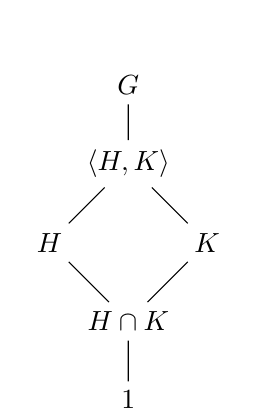
\begin{tikzpicture}
            \node (G) at (0, 0) {$G$};
            \node (HK) at (0, -1) {$\gen{H, K}$};
            \node (H) at (-1, -2) {$H$};
            \node (K) at (1, -2) {$K$};
            \node (HnK) at (0, -3) {$H \cap K$};
            \node (1) at (0, -4) {$1$};

            \draw (G) -- (HK) -- (H) -- (HnK) -- (1);
            \draw (HK) -- (K) -- (HnK);
        \end{tikzpicture}
    \end{center}
    If $H \leq K$, then the sublattice is a chain, noting that $\gen{H, K} = K$ and $H \cap K = H$. If $H = K$, then the sublattice is also a chain, noting that $\gen{H, K} = H = K$ and $H \cap K = H = K$:
    \begin{center}
        \begin{tikzpicture}
            \node(G) at (0, 0) {$G$};
            \node(K) at (0, -1) {$K$};
            \node(H) at (0, -2) {$H$};
            \node(1) at (0, -3) {$1$};

            \node(G2) at (4, 0) {$G$};
            \node(HK) at (4, -1) {$H = K$};
            \node(12) at (4, -2) {$1$};

            \draw (G) -- (K) -- (H) -- (1);
            \draw (G2) -- (HK) -- (12);
        \end{tikzpicture}
    \end{center}
    Remaining scenarios include more trivial cases where one of $H$ or $K$ is either $G$ or $1$.
\end{sol}

\begin{exercise}
    In each of (a) to (d) list all subgroups of $D_{16}$ that satisfy the given condition.
    \begin{subproblems}
        \item Subgroups that are contained in $\gen{sr^2, r^4}$
        \item Subgroups that are contained in $\gen{sr^7, r^4}$
        \item Subgroups that contain $\gen{r^4}$
        \item Subgroups that contain $\gen s$.
    \end{subproblems}
\end{exercise}

\begin{sol}
    Using the subgroup lattice of $D_{16}$, we find:
    \begin{subproblems}
        \item $\gen{sr^2, r^4}, \gen {sr^6}, \gen{sr^2}, \gen{r^4}, 1$.
        \item Note $sr^7 = sr^3$, so $\gen{sr^3, r^4}, \gen{r^4}, \gen{sr^3}, \gen{sr^7}, 1$.
        \item $\gen{r^4}, \gen{sr^2, r^4}, \gen{s, r^4}, \gen{r^2}, \gen{sr^3, r^4}, \gen{sr^5, r^4}, \gen{s, r^2}, \gen r, \gen{sr, r^2}, D_{16}$.
        \item $\gen s, \gen{s, r^4}, \gen{s, r^2}, D_{16}$. \qh
    \end{subproblems}
\end{sol}

\newpage

\begin{exercise}
    Show that the subgroup $\gen{s, r^2}$ of $D_8$ is isomorphic to $V_4$.
\end{exercise}

\begin{sol}
    Recall that $V_4 = \set{1, a, b, c}$ where $a^2 = b^2 = c^2 = 1$ and $ab = c$, $bc = a$, and $ca = b$. Note that every element in $\gen{s, r^2}$ has order 2 since $(r^2)^2 = s^2 = 1$ and $(sr^2)^2 = sr^2sr^2 = 1$. Then we may define a mapping $\phi : V_4 \to \gen{s, r^2}$ by
    \[\phi(1) = 1, \quad \phi(a) = s, \quad \phi(b) = r^2, \quad \phi(c) = sr^2\]
    We show that $\phi$ is a homomorphism by checking the products:
    \begin{align*}
        \phi(a^2) & = \phi(1) = 1 = s^2 = \phi(a)^2 \\
        \phi(b^2) & = \phi(1) = 1 = (r^2)^2 = \phi(b)^2 \\
        \phi(ab) & = \phi(c) = sr^2 = \phi(a)\phi(b)
    \end{align*}
    Similar calculations show that $\phi(bc) = \phi(b)\phi(c)$ and $\phi(ca) = \phi(c)\phi(a)$. Since $\phi$ is defined on all elements of $V_4$, then $\phi$ is a homomorphism. Moreover, $\phi$ is surjective since $\phi(V_4) = \gen{s, r^2}$. Since $\abs{V_4} = \abs{\gen{s, r^2}} = 4$, then $\phi$ is injective as well. Therefore, $\gen{s, r^2} \cong V_4$.
\end{sol}

\begin{exercise}
    Use the given lattice to find all pairs of elements that generate $D_8$ (there are 12 pairs).
\end{exercise}

\begin{sol}
    Note that $D_8 = \gen{s, r}$. Moreover, $s \neq rs$, and $r \in \gen{s, rs}$ so that $\gen{s, rs} = D_8$. Since $r = r^3$, we also have $\gen{s, r^3} = D_8$. We may also replace the reflection $s$ with $sr^2$, since combinations of a reflection with an odd rotation and a reflection with an even rotation contain $r$ and thus generates $D_8$. It follows that the pairs of elements that generate $D_8$ are:
    \[\gen{s, r}, \gen{s, r^3}, \gen{s, rs}, \gen{s, r^3s}, \gen{r^2s, r}, \gen{r^2s, r^3}, \gen{r^2s, rs}, \gen{r^2s, r^3s}, \gen{r, rs}, \gen{r^3, rs}, \gen{r, r^3s}, \gen{r^3, r^3s} \qh\]
\end{sol}

\begin{exercise}
    Use the given lattice to find all elements $x \in D_{16}$ such that $D_{16} = \gen{x, s}$ (there are 8 such elements $x$).
\end{exercise}

\begin{sol}
    Note that $\gen r= \gen{r^3} = \gen{r^5} = \gen{r^7}$. We then pair each generator with an $s$ so that we obtain just the rotation to then generate $D_{16}$: $x = r, r^3, r^5, r^7, sr, sr^3, sr^5, sr^7$.
\end{sol}

\begin{exercise}
    Use the given lattices to help find the centralizers of every element in the following groups:
    \begin{subproblems}
        \item $D_8$ \quad (b) $Q_8$ \quad (c) $S_3$ \quad (d) $D_{16}$.
    \end{subproblems}
\end{exercise}

\begin{solalph}
    \item To calculate the centralizer of an element $a$, start with the cyclic subgroup that contains $a$ and see if any other elements are contained in $\gen a$. For example, to calculate $C_{D_8}(rs)$, start with $\gen{rs}$ in the subgroup lattice. Since $r^4, sr^5 \in C_{D_8}(rs)$, then $C_{D_8}(rs) \leq \gen{sr^5, r^4}$. Checking the next subgroup, it follows that $r^2 \in C_{D_8}(rs)$ so that $C_{D_8}(rs) \leq \gen{rs, r^2}$. Since $r \not\in C_{D_8}(rs)$, then $C_{D_8}(rs) \neq D_{16}$ so that $C_{D_8}(rs) = \gen{rs, r^2}$. We use similar reasoning to deduce the other centralizers:
    \begin{align*}
        C_{D_8}(1) & = D_8 & C_{D_8}(s) & = \gen{s, r^2} \\
        C_{D_8}(r) & = \gen r & C_{D_8}(rs) & = \gen{rs, r^2} \\
        C_{D_8}(r^2) & = D_8 & C_{D_8}(r^2s) & = \gen{s, r^2} \\
        C_{D_8}(r^3) & = \gen r & C_{D_8}(r^3s) & = \gen{sr, r^2}
    \end{align*}
    \item Note that $1, -1 \in Z(Q_8)$, while none of $i, j$, and $k$ commute with anything but themselves. Then:
    \begin{align*}
        C_{Q_8}(1) & = C_{Q_8}(-1) = Q_8 \\
        C_{Q_8}(i) & = C_{Q_8}(-i) = \gen i \\
        C_{Q_8}(j) & = C_{Q_8}(-j) = \gen j \\
        C_{Q_8}(k) & = C_{Q_8}(-k) = \gen k
    \end{align*}
    \item Since no element in $S_3$ commutes with each other, then $C_{S_3}(a) = \gen a$ for all $a \in S_3 - \set 1$, where $C_{S_3}(1) = S_3$.
    \item Use similar reasoning as in part (a) to obtain the centralizers:
    \begin{align*}
        C_{D_{16}}(1) = C_{D_{16}}(r^4) & = D_{16} \\
        C_{D_{16}}(r^k) & = \gen r \text{ for all $k = 1, 2, 3, 5, ,6, $} \\
        C_{D_{16}}(s) = C_{D_{16}}(sr^4) & = \gen{s, r^4} \\
        C_{D_{16}}(sr) = C_{D_{16}}(sr^5) & = \gen{sr^5, r^4} \\
        C_{D_{16}}(sr^2) = C_{D_{16}}(sr^6) & = \gen{sr^2, r^4} \\
        C_{D_{16}}(sr^3) = C_{D_{16}}(sr^7) & = \gen{sr^3, r^4} \qh
    \end{align*}
\end{solalph}

\begin{exercise}
    Find the center of $D_{16}$.
\end{exercise}

\begin{sol}
    $Z(D_{16}) = \set{1, r^4}$ by \hyperref[ex2.2.7]{Exercise 2.2.7}.
\end{sol}

\begin{exercise}
    In each of the following groups find the normalizer of each subgroup:
    \begin{subproblems}
        \item $S_3$ \quad (b)~~$Q_8$.
    \end{subproblems}
\end{exercise}

\begin{solalph}
    \item From the subgroup lattice of $S_3$, we can deduce that each subgroup is cyclic and maximal except for $\set\id$, where $N_{S_3}(\id) = S_3$. Then for any $\alpha \in S_3$, we observe that $N_{S_3}(\gen\alpha) = \gen\alpha$ or $S_3$.
    
    Consider $\alpha = (1\ 2)$. Since $(1\ 3)(1\ 2)(1\ 3) = (2\ 3) \not\in \gen{(1\ 2)}$, then $N_{S_3}(\gen{(1\ 2)}) \neq S_3$ so that $N_{S_3}(\gen{(1\ 2)}) = \gen{(1\ 2)}$. By symmetry, the same holds for $\gen{(1\ 3)}$ and $\gen{(2\ 3)}$.

    Consider $\alpha = (1\ 2\ 3)$. Observe that
    \[(1\ 2)(1\ 2\ 3)(1\ 2) = (1\ 3\ 2) \longand (1\ 2)(1\ 3\ 2)(1\ 2) = (1\ 2\ 3)\]
    so that $(1\ 2) \in N_{S_3}(\gen{(1\ 2\ 3)})$. Then $N_{S_3}(\gen{(1\ 2\ 3)}) = S_3$.
    \item Note that the subgroups $\gen{-1}$ and $\set 1$ are normal in $Q_8$ so that $N_{Q_8}(\gen{-1}) = N_{Q_8}(\set 1) = Q_8$. Consider the subgroups of order 4 in $Q_8$. In particular, observe for $i$:
    \[jij\inv = -i, j(-i)j\inv = i\]
    so that $j \in N_{Q_8}(\gen i)$. Then $N_{Q_8}(\gen i) = Q_8$. By symmetry, the same holds for $\gen j$ and $\gen k$.
\end{solalph}

\newpage

\begin{exercise}
    Draw the lattices of subgroups of the following groups:
    \begin{subproblems}
        \item $\intmod[16]$ \quad (b)~~$\intmod[24]$ \quad (c)~~$\intmod[48]$.
    \end{subproblems}
\end{exercise}

\begin{solalph}
    \item $\intmod[16]$
    \begin{center}
        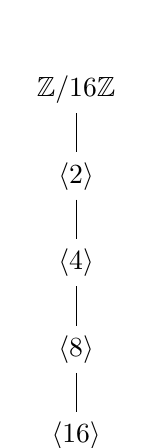
\begin{tikzpicture}[every node/.style=on grid, node distance=1.1cm]
            \node (g) {$\intmod[16]$};
            \node (2) [below=of g] {$\gen 2$};
            \node (4) [below=of 2] {$\gen 4$};
            \node (8) [below=of 4] {$\gen 8$};
            \node (16) [below=of 8] {$\gen{16}$};

            \draw (g) -- (2) -- (4) -- (8) -- (16);
        \end{tikzpicture}
    \end{center}
    \item $\intmod[24]$
    \begin{center}
        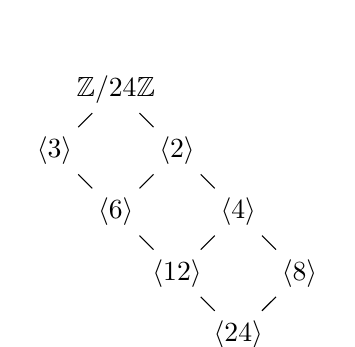
\begin{tikzpicture}[every node/.style=on grid, node distance=1.1cm]
            \node (g) {$\intmod[24]$};
            \node (3) [below left=of g] {$\gen 3$};
            \node (2) [below right=of g] {$\gen 2$};
            \node (6) [below right=of 3] {$\gen 6$};
            \node (4) [below right=of 2] {$\gen 4$};
            \node (12) [below right=of 6] {$\gen{12}$};
            \node (8) [below right=of 4] {$\gen 8$};
            \node (24) [below right=of 12] {$\gen{24}$};

            \draw (g) -- (3) -- (6) -- (12) -- (24);
            \draw (g) -- (2) -- (4) -- (8) -- (24);
            \draw (6) -- (2);
            \draw (12) -- (4);
        \end{tikzpicture}
    \end{center}
    \item $\intmod[48]$
    \begin{center}
        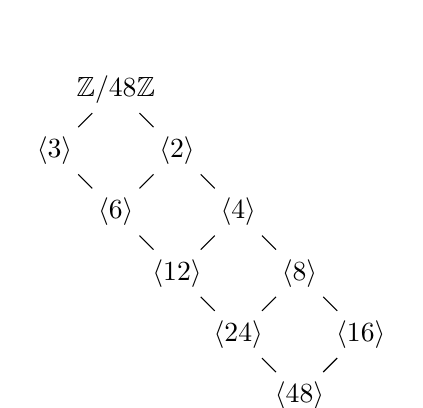
\begin{tikzpicture}[every node/.style=on grid, node distance=1.1cm]
            \node (g) {$\intmod[48]$};
            \node (3) [below left=of g] {$\gen 3$};
            \node (2) [below right=of g] {$\gen 2$};
            \node (6) [below right=of 3] {$\gen 6$};
            \node (4) [below right=of 2] {$\gen 4$};
            \node (12) [below right=of 6] {$\gen{12}$};
            \node (8) [below right=of 4] {$\gen 8$};
            \node (24) [below right=of 12] {$\gen{24}$};
            \node (16) [below right=of 8] {$\gen{16}$};
            \node (48) [below right=of 24] {$\gen{48}$};

            \draw (g) -- (3) -- (6) -- (12) -- (24) -- (48);
            \draw (g) -- (2) -- (4) -- (8) -- (16) -- (48);
            \draw (6) -- (2);
            \draw (12) -- (4);
            \draw (24) -- (8);
        \end{tikzpicture}
    \end{center}
\end{solalph}

\begin{exercise}
    Classify groups of order 4 by proving that if $\abs G = 4$, then $G \cong Z_4$ or $G \cong V_4$. [See \hyperref[ex1.1.36]{Exercise 1.1.36}.]
\end{exercise}

\begin{sol}
    Let $G = \set{1, a, b, c}$.  If $G$ has an element of order 4, then $G \cong Z_4$ by Theorem 2.4.

    Suppose $G$ is not cyclic. Then every nonidentity element has order 2 by Lagrange's Theorem. In particular, $a^2 = b^2 = c^2 = 1$. Note that $ab \neq 1$, since otherwise $b = a\inv = a$. Similarly, $ab \neq a$ and $ab \neq b$, so that $ab = c$. By similar reasoning, we have $bc = a$ and $ca = b$. This is precisely the definition of $V_4$, so that $G \cong V_4$.
\end{sol}

\newpage

\begin{exercise} \label{ex2.5.11} 
    Consider the group of order 16 with the following presentation:
    \[QD_{16} = \gen{\sigma, \tau \mid \sigma^8 = \tau^2 = 1, \sigma\tau = \tau\sigma^3}\]
    (called the \textit{quasidihedral} or \textit{semidihedral} group of order 16). This group has three subgroups of order 8: $\gen{\tau, \sigma^2} \cong D_8, \gen \sigma \cong Z_8$, and $\gen{\sigma^2, \sigma\tau} \cong Q_8$, and every proper subgroup is contained in one of these three subgroups. Fill in the missing subgroups in the lattice of all subgroups of the quasidihedral group, exhibiting each subgroup with at most two generators.
    \begin{center}
        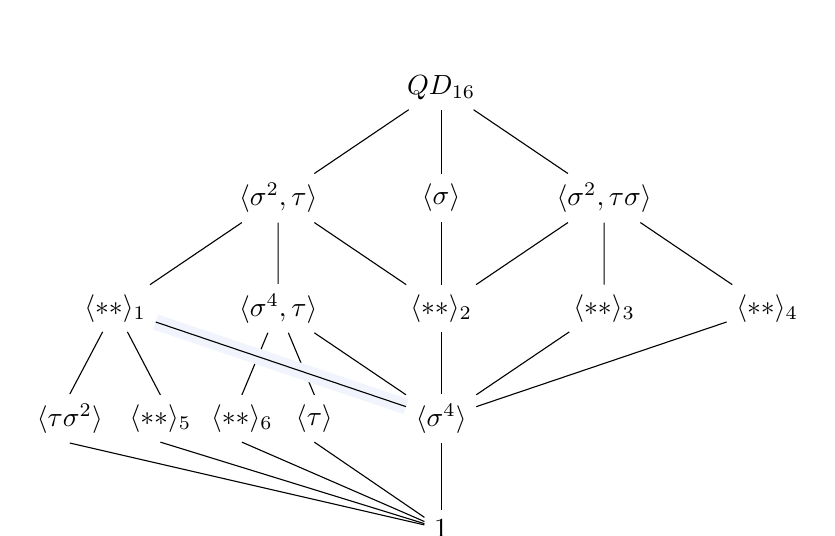
\begin{tikzpicture}[xscale=1.15, yscale=1.4]
            \node (G) at (0, 0) {$QD_{16}$};

            \node (s2t) at (-1.8, -1) {$\gen{\sigma^2, \tau}$};
            \node (s) at (0, -1) {$\gen \sigma$};
            \node (s2ts) at (1.8, -1) {$\gen{\sigma^2, \tau\sigma}$};

            \node (u1) at (-3.6, -2) {$\gen{**}_1$};
            \node (s4t) at (-1.8, -2) {$\gen{\sigma^4, \tau}$};
            \node (u2) at (0, -2) {$\gen{**}_2$};
            \node (u3) at (1.8, -2) {$\gen{**}_3$};
            \node (u4) at (3.6, -2){$\gen{**}_4$};

            \node (ts2) at (-4.1, -3) {$\gen{\tau\sigma^2}$};
            \node (u5) at (-3.1, -3) {$\gen{**}_5$};
            \node (u6) at (-2.2, -3) {$\gen{**}_6$};
            \node (t) at (-1.4, -3){$\gen \tau$};
            \node (s4) at (0, -3) {$\gen{\sigma^4}$};

            \node (1) at (0, -4) {1};

            \draw (1) -- (ts2.south);
            \draw (ts2.north) -- (u1) -- (s2t) -- (G);
            \draw (1) -- (u5.south);
            \draw (u5.north) -- (u1);
            \draw (1) -- (u6.south);
            \draw (u6.north) -- (s4t) -- (s2t);
            \draw (1) -- (t.south);
            \draw (t.north) -- (s4t);
            \draw (1) -- (s4) -- (u2) -- (s) -- (G);
            \draw [preaction={draw, line width=2mm, color=RoyalBlue!7}] (s4) -- (u1);
            \draw (s4) -- (s4t);
            \draw (s4) -- (u3) -- (s2ts) -- (G);
            \draw (s4) -- (u4) -- (s2ts);
            \draw (u2) -- (s2t);
            \draw (u2) -- (s2ts);
        \end{tikzpicture}
    \end{center}
\end{exercise}

\begin{sol}
    The above has had subscripts added to distinguish the unknown subgroups. It is clear that $\gen{**}_2$ must be $\gen{\sigma^2}$ since it is the only subgroup contained in both $\gen \sigma$ and $\gen{\sigma^2, \tau}$. To find the other subgroups, we calculate the cyclic subgroups of the form $\gen{\tau\sigma^k}$:
    \begin{align*}
        \gen{\tau\sigma} & = \set{1, \tau\sigma, \sigma^4, \tau\sigma^5} & \gen{\tau\sigma^3} & = \set{1, \tau\sigma^3, \sigma^4, \tau\sigma^7} \\
        \gen{\tau\sigma^4} & = \set{1, \tau\sigma^4} & \gen{\tau\sigma^6} & = \set{1, \tau\sigma^6}
    \end{align*}
    It becomes clear that 6 must be $\gen{\tau\sigma^4}$, since the subgroup above contains both $\tau$ and $\sigma^4$. 3 and 4 must be $\gen{\tau\sigma}$ and $\gen{\tau\sigma^3}$ respectively, since $\gen{\sigma^2, \tau\sigma}$ both contain $\tau\sigma$ and $\sigma^2$ which multiply to $\tau\sigma^3$. Certainly, 1 cannot be $\gen{\tau\sigma^6}$ as it does not contain $\gen{\tau\sigma^2}$, so it must be 5. Then 1 must be $\gen{\tau\sigma^2, \sigma^4}$ as it contains both subgroups. Hence, the completed diagram is
    \begin{center}
        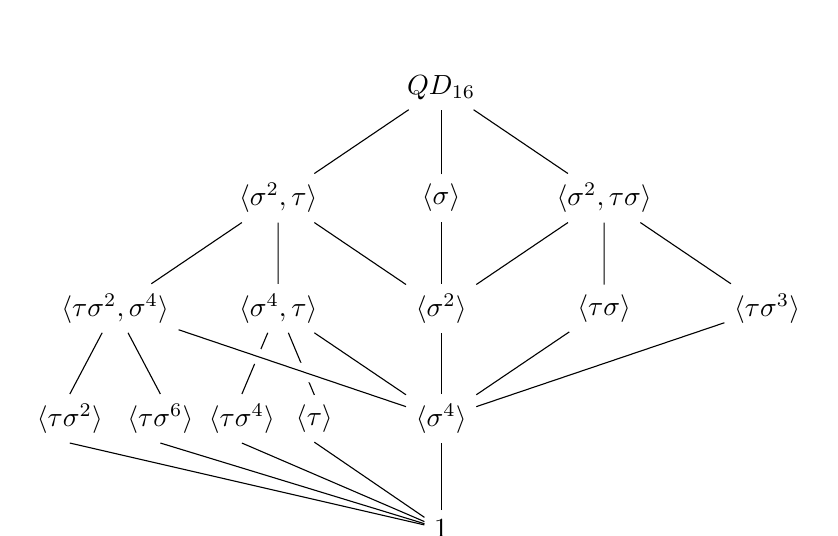
\begin{tikzpicture}[xscale=1.15, yscale=1.4]
            \node (G) at (0, 0) {$QD_{16}$};

            \node (s2t) at (-1.8, -1) {$\gen{\sigma^2, \tau}$};
            \node (s) at (0, -1) {$\gen \sigma$};
            \node (s2ts) at (1.8, -1) {$\gen{\sigma^2, \tau\sigma}$};

            \node (u1) at (-3.6, -2) {$\gen{\tau\sigma^2, \sigma^4}$};
            \node (s4t) at (-1.8, -2) {$\gen{\sigma^4, \tau}$};
            \node (u2) at (0, -2) {$\gen{\sigma^2}$};
            \node (u3) at (1.8, -2) {$\gen{\tau\sigma}$};
            \node (u4) at (3.6, -2){$\gen{\tau\sigma^3}$};

            \node (ts2) at (-4.1, -3) {$\gen{\tau\sigma^2}$};
            \node (u5) at (-3.1, -3) {$\gen{\tau\sigma^6}$};
            \node (u6) at (-2.2, -3) {$\gen{\tau\sigma^4}$};
            \node (t) at (-1.4, -3){$\gen \tau$};
            \node (s4) at (0, -3) {$\gen{\sigma^4}$};

            \node (1) at (0, -4) {1};

            \draw (1) -- (ts2.south);
            \draw (ts2.north) -- (u1) -- (s2t) -- (G);
            \draw (1) -- (u5.south);
            \draw (u5.north) -- (u1);
            \draw (1) -- (u6.south);
            \draw (u6.north) -- (s4t) -- (s2t);
            \draw (1) -- (t.south);
            \draw (t.north) -- (s4t);
            \draw (1) -- (s4) -- (u2) -- (s) -- (G);
            \draw [preaction={draw, line width=2mm, white}] (s4) -- (u1);
            \draw (s4) -- (s4t);
            \draw (s4) -- (u3) -- (s2ts) -- (G);
            \draw (s4) -- (u4) -- (s2ts);
            \draw (u2) -- (s2t);
            \draw (u2) -- (s2ts);
        \end{tikzpicture}
    \end{center}
\end{sol}

\begin{exercise} \label{ex2.5.12} 
    The group $A = Z_2 \times Z_4 = \gen{a, b \mid a^2 = b^4 = 1, ab = ba}$ has order 8 and has three subgroups of order 4: $\gen{a, b^2} \cong V_4, \gen b \cong Z_4$, and $\gen{ab} \cong Z_4$ and every proper subgroup is contained in one of these three. Draw the lattice of all subgroups of $A$, giving each subgroup in terms of at most two generators.
\end{exercise}

\begin{sol}
    Observe that $A$ is the direct product of two abelian groups, so $A$ is abelian, and we may write it as
    \[A = \set{1, a, b, b^2, b^3, ab, ab^2, ab^3}\]
    We know that $A$ has three subgroups of order 4: $\gen{a, b^2}, \gen b$, and $\gen{ab}$. To find what the containment relations are, observe that $\gen{a, b}^2$ has three subgroups of order 2: $\gen{b^2}, \gen a$, and $\gen{ab^2}$. $\gen b$ has the single subgroup of order 2: $\gen{b^2}$, and $\gen{ab}$ has the single subgroup of order 2: $\gen{ab^2}$. Then the subgroup lattice of $A$ is
    \begin{center}
        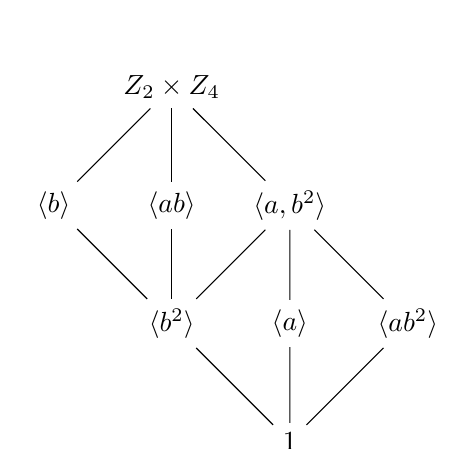
\begin{tikzpicture}[scale=1.5]
            \node (A) at (0, 0) {$Z_2 \times Z_4$};
            
            \node (b) at (-1, -1) {$\gen b$};
            \node (ab) at (0, -1) {$\gen{ab}$};
            \node (a b2) at (1, -1) {$\gen{a, b^2}$};

            \node (b2) at (0, -2) {$\gen{b^2}$};
            \node (a) at (1, -2) {$\gen a$};
            \node (ab2) at (2, -2) {$\gen{ab^2}$};

            \node (1) at (1, -3) {1};

            \draw (1) -- (b2) -- (b) -- (A);
            \draw (1) -- (a) -- (a b2) -- (A);
            \draw (b2) -- (ab) -- (A);
            \draw (b2) -- (a b2);
            \draw (1) -- (ab2) -- (a b2);
        \end{tikzpicture}
    \end{center}
\end{sol}

\begin{exercise} \label{ex2.5.13}
    The group $G = Z_2 \times Z_8 = \gen{x, y \mid x^2 = y^8 = 1, xy = yx}$ has order 16 and has three subgroups of order 8: $\gen{x, y^2} \cong Z_2 \times Z_4, \gen y \cong Z_8$, and $\gen{xy} \cong Z_8$, and every proper subgroup is contained in one of those three. Draw the lattice of all subgroups of $G$, giving each subgroups in terms of at most two generators (cf. \hyperref[ex2.5.12]{Exercise 2.5.12}).
\end{exercise}

\begin{sol}
    Let $x = a$ and $y^2 = b$, where $a$ and $b$ are the generators from \hyperref[ex2.5.12]{Exercise 2.5.12}. It follows that $G$ contains a copy of $Z_2 \times Z_4$ as $\gen{x, y^2} = \gen{a, b}$. Moreover, we may append $\gen y$ and $\gen{xy}$ to this lattice as follows:
    \begin{center}
        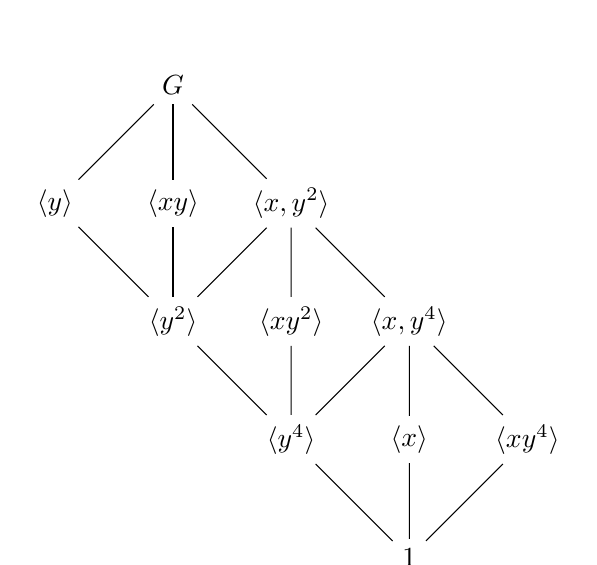
\begin{tikzpicture}[scale = 1.5]
            \node (G) at (0, 0) {$G$};

            \node (y) at (-1, -1) {$\gen y$};
            \node (xy) at (0, -1) {$\gen{xy}$};
            \node (x y2) at (1, -1) {$\gen{x, y^2}$};

            \node (y2) at (0, -2) {$\gen{y^2}$};
            \node (xy2) at (1, -2) {$\gen{xy^2}$};
            \node (x y4) at (2, -2) {$\gen{x, y^4}$};

            \node (y4) at (1, -3) {$\gen{y^4}$};
            \node (x) at (2, -3) {$\gen x$};
            \node (xy4) at (3, -3) {$\gen{xy^4}$};

            \node (1) at (2, -4) {1};

            \draw (1) -- (y4) -- (y2) -- (y) -- (G);
            \draw (1) -- (xy4) -- (x y4) -- (x y2) -- (G);
            \draw (1) -- (x) -- (x y4);
            \draw (y4) -- (xy2) -- (x y2);
            \draw (y2) -- (xy) -- (G);
            \draw (y4) -- (x y4);
            \draw (y2) -- (x y2);
        \end{tikzpicture}
    \end{center}
\end{sol}

\begin{exercise} \label{ex2.5.14} 
    Let $M$ be the group of order 16 with the following presentation:
    \[\gen{u, v \mid u^2 = v^8 = 1, vu = uv^5}\]
    (sometimes called the \textit{modular} group of order 16). It has three subgroups of order 8: $\gen{u, v^2}, \gen v$, and $\gen{uv}$, and every proper subgroup is contained in one of those three. Prove that $\gen{u, v^2} \cong Z_2 \times Z_4, \gen v \cong Z_8$, and $\gen{uv} \cong Z_8$. Show that the lattice of subgroups of $M$ is the same as the lattice of subgroups of $Z_2 \times Z_8$ (cf. Exercise 13) but that these two groups are not isomorphic.
\end{exercise}

\begin{sol}
    It is clear that $\abs v = 8$ implies that $\gen v \cong Z_8$. Similarly, since $\abs{uv} = 8$, then $\gen{uv} \cong Z_8$. To see that $\gen{u, v^2} \cong Z_2 \times Z_4$, we verify the relations. Note that $u^2 = (v^2)^4 = 1$, and
    \[v^2u = vuv^5 = uv^{10} = uv^2\]
    so that $u$ and $v^2$ commute, hence it is abelian. We may then list out the elements of $\gen{u, v^2}$:
    \[\gen{u, v^2} = \set{1, v^2, v^4, v^6, u, uv^2, uv^4, uv^6}\]
    Then the mapping $\phi : Z_2 \times Z_4 \to \gen{u, v^2}$ defined by
    \[\phi(a) = u, \quad \phi(b) = v^2\]
    extends to a homomorphism. Moreover, it is clear that distinct elements in $Z_2 \times Z_4$ map to distinct elements in $\gen{u, v^2}$, so that $\phi$ is injective. As shown above, $|\gen{u, v^2}| = 8 = |Z_2 \times Z_4|$, so that $\phi$ is surjective. Hence, $\phi$ is an isomorphism and $Z_2 \times Z_4 \cong \gen{u, v^2}$. The subgroup lattice of $M$ is then the same as that of $Z_2 \times Z_8$ as shown in \hyperref[ex2.5.13]{Exercise 2.5.13}, but with $u = x$ and $v = y$:
    \begin{center}
        \begin{tikzpicture}[scale = 1.5]
            \node (G) at (0, 0) {$G$};

            \node (y) at (-1, -1) {$\gen v$};
            \node (xy) at (0, -1) {$\gen{uv}$};
            \node (x y2) at (1, -1) {$\gen{u, v^2}$};

            \node (y2) at (0, -2) {$\gen{v^2}$};
            \node (xy2) at (1, -2) {$\gen{uv^2}$};
            \node (x y4) at (2, -2) {$\gen{u, v^4}$};

            \node (y4) at (1, -3) {$\gen{v^4}$};
            \node (x) at (2, -3) {$\gen u$};
            \node (xy4) at (3, -3) {$\gen{uv^4}$};

            \node (1) at (2, -4) {1};

            \draw (1) -- (y4) -- (y2) -- (y) -- (G);
            \draw (1) -- (xy4) -- (x y4) -- (x y2) -- (G);
            \draw (1) -- (x) -- (x y4);
            \draw (y4) -- (xy2) -- (x y2);
            \draw (y2) -- (xy) -- (G);
            \draw (y4) -- (x y4);
            \draw (y2) -- (x y2);
        \end{tikzpicture}
    \end{center}
    Finally, $M$ is not isomorphic to $Z_2 \times Z_8$ since $M$ is not abelian. If it were, then $vu = uv$, but $vu = uv^5 = uv$ would imply that $v^4 = 1$, contradicting that $\abs v = 8$.
\end{sol}

\newpage

\begin{exercise}
    Describe the isomorphism type of each of the three subgroups of $D_{16}$ of order 8.
\end{exercise}

\begin{sol}
    Since $\abs r = 8$, then $\gen r \cong Z_8$. For the remaining subgroups, note that the lattice for $D_{16}$ shows a striking similarity to the lattice for $D_8$; in fact, these subgroups \textit{are} isomorphic to $D_8$ as follows:
    
    For the subgroup $\gen{s, r^2}$, observe that $(r^2)4 = s^2 = 1$, and $sr^2 = r^6s = (r^2)\inv s$. Then the mapping $\phi : D_8 \to \gen{s, r^2}$ given by
    \[\phi(r) = r^2, \quad \phi(s) = s\]
    extends to a homomorphism. Moreover, this mapping is surjective by construction. Since $\gen{s, r^2}$ contains a subgroup of order 4 and is a subgroup of $D_{16}$, it must be 8 so that $\phi$ is an isomorphism, and $D_8 \cong \gen{s, r^2}$.
    
    For the subgroup $\gen{sr, r^2}$, we again observe that $(r^2)^4 = (sr)^2 = 1$, and $(sr)r^2 = sr^3 = r^5s = r^6r^7s = (r^2)\inv(sr)$. The mapping $\psi : D_8 \to \gen{sr, r^2}$ given by
    \[\phi(r) = r^2, \phi(s) = sr\]
    extends to a homomorphism, surjective by construction, and is an isomorphism because $\gen{sr, r^2}$ has order 8. Then $D_8 \cong \gen{sr, r^2}$.
\end{sol}

\begin{exercise}
    Use the lattice of subgroups of the quasidihedral of order 16 to show that every element of order 2 is contained in the proper subgroup $\gen{\tau, \sigma^2}$ (cf. \hyperref[ex2.5.11]{Exercise 2.5.11}).
\end{exercise}

\begin{sol}
    Every element of order 2 generates a cyclic subgroup of order 2. Using the lattice, $\gen{\tau, \sigma^2}$ properly contains all cyclic subgroups, except $\gen{\tau\sigma}$ and $\gen{\tau\sigma^3}$, both of which are order 4. Then $\gen{\tau, \sigma^2}$ contains all cyclic subgroups of order 2, hence contain all elements of order 2.
\end{sol}

\begin{exercise}
    Use the lattice of subgroups of the modular group $M$ of order 16 to show that the set $\set{x \in M \mid x^2 = 1}$ is a subgroup of $M$ isomorphic to the Klein 4-group (cf. \hyperref[ex2.5.14]{Exercise 2.5.14}).
\end{exercise}

\begin{sol}
    Using the lattice in Exercise 14, we see that we have 3 candidates to be isomorphic to $V_4$, namely $\gen{v^2}, \gen{uv^2},$ and $\gen{u, v^4}$. The first and second subgroups are cyclic, while $\gen{u, v^4} = \set{1, u, v^4, uv^4}$. Since it is not generated by one element, each of these elements are of order 2, and $v^4u = v^3uv^5 = \cdots = uv^{20} = uv^4$ so that it is abelian, then $\gen{u, v^4} \cong V_4$.
\end{sol}

\begin{exercise}
    Use the lattice to help find the centralizer of every element of $QD_{16}$ (cf. \hyperref[ex2.5.11]{Exercise 2.5.11}).
\end{exercise}

\begin{sol}
    Note that $\sigma^4\tau = \sigma^3\tau\sigma^3 = \cdots = \tau\sigma^{12} = \tau\sigma^4$ so that $\sigma^4 \in Z(QD_{16})$ as $\sigma^4$ already commutes with powers of $\sigma$. Moreover, any power of $\sigma$ does not commute with $\tau$ except for $\sigma^4$. The elements $\tau\sigma$ and $\tau\sigma^3$ do not commute with $\sigma^2$ as $(\tau\sigma)\sigma^2 = \tau\sigma^3 = \sigma\tau \neq \sigma^2(\tau\sigma) = \tau\sigma^2$, and $(\tau\sigma^3)\sigma^2 = \sigma^7\tau \neq \sigma^3\tau = \sigma^2(\tau\sigma^3)$. Next, $(\tau\sigma^2)\sigma^2 = \tau\sigma^4 \neq \tau = \sigma^2(\tau\sigma^2)$ so that $\sigma^2$ does not commute with $\tau\sigma^2$. Moreover, $(\tau\sigma^6)(\tau\sigma^2) = \tau\sigma^2\sigma^4\tau\sigma^2 = (\tau\sigma^2)(\tau\sigma^6)$ so that $\tau\sigma^2$ commutes with $\tau\sigma^6$, but $\sigma^2\tau\sigma^6 = \tau\sigma^4 \neq \tau = (\tau\sigma^6)\sigma^2$ so $\sigma^2$ does not commute with $\tau\sigma^6$. Lastly, $\sigma^2(\tau\sigma^4) = \tau\sigma^2 \neq (\tau\sigma^4)\sigma^2$, and $\sigma^2\tau = \tau\sigma^6 \neq \tau\sigma^2$ so that $\sigma^2$ does not commute with $\tau\sigma^4$ nor with $\tau$. It follows that the centralizers of the elements of $QD_{16}$ are
    \begin{align*}
        C_{QD_{16}}(1) = C_{QD_{16}}(\sigma^4) & = QD_{16} \\
        C_{QD_{16}}(\gen{\sigma^k}) & = \gen\sigma \text{ for $k = 1, 2, 3, 5, 6, 7$} \\
        C_{QD_{16}}(\gen{\tau\sigma}) = C_{QD_{16}}(\gen{\tau\sigma^5}) & = \gen{\tau\sigma} \\
        C_{QD_{16}}(\gen{\tau\sigma^3}) = C_{QD_{16}}(\gen{\tau\sigma^7}) & = \gen{\tau\sigma^3} \\
        C_{QD_{16}}(\gen\tau) = C_{QD_{16}}(\gen{\tau\sigma^4}) & = \gen{\sigma^4, \tau} \\
        C_{QD_{16}}(\gen{\tau\sigma^2}) = C_{QD_{16}}(\gen{\tau\sigma^6}) & = \gen{\tau\sigma^2, \sigma^4}
    \end{align*}
\end{sol}

\begin{exercise}
    Use the lattice to help find $N_{D_{16}}(\gen{s, r^4})$.
\end{exercise}

\begin{sol}
    Based on the placement of $\gen{s, r^4}$, its normalizer may be itself, $\gen{s, r^2}$, or $D_{16}$. Note that $\gen{s, r^4} = \{1, s, r^4, sr^4\}$, and taking $r^2$ and $(r^2)\inv = r^6$, we have
    \[r^2\gen{s, r^4}r^6 = \set{1, sr^4, r^4, s} = \gen{s, r^4}\]
    so that $r^2 \in N_{D_{16}}(\gen{s, r^4})$, and $\gen{s, r^2} \leq N_{D_{16}}(\gen{s, r^4})$. Since $rsr\inv = r^2s \neq r$, then $r \not\in N_{D_{16}}(\gen{s, r^4})$ so that $N_{D_{16}}(\gen{s, r^4}) = \gen{s, r^2}$.
\end{sol}

\begin{exercise}
    Use the lattice of subgroups of $QD_{16}$ (cf. \hyperref[ex2.5.11]{Exercise 2.5.11}) to help find the normalizers
    \begin{subproblems}
        \item $N_{QD_{16}}(\gen{\tau\sigma})$ \quad (b)~~$N_{QD_{16}}(\gen{\tau, \sigma^4})$.
    \end{subproblems}
\end{exercise}

\begin{solalph}
    \item Note that $\gen{\tau\sigma} = \set{1, \tau\sigma, \sigma^4, \tau\sigma^5}$. Moreover, $(\sigma^2)\inv = \sigma^6$ so that
    \[\sigma^2\gen{\tau\sigma}\sigma^6 = \{1, \tau\sigma^4, \sigma^4, \tau\sigma\} = \gen{\tau\sigma}\]
    and $\sigma(\tau\sigma)\sigma^7 = \tau\sigma^3 \neq \tau\sigma$ so that $\sigma \not\in N_{QD_{16}}(\gen{\tau\sigma})$. Then $N_{QD_{16}}(\gen{\tau\sigma}) = \gen{\sigma^2, \tau\sigma}$.
    \item $\gen{\tau, \sigma^4} = \{1, \tau, \sigma^4, \tau\sigma^4\}$, and 
    \[\sigma^2\gen{\tau, \sigma^4}\sigma^6 = \{1, \tau\sigma^4, \sigma^4, \tau\}\]
    while $\sigma\tau\sigma^7 = \tau\sigma^2 \neq \tau$ so that $\sigma \not\in N_{QD_{16}}(\gen{\tau, \sigma^4})$. Then $N_{QD_{16}}(\gen{\tau, \sigma^4}) = \gen{\sigma^2, \tau}$.
\end{solalph}
\section{Quotient Groups and Homomorphisms}

\subsection{Definitions and Examples}

Let $G$ and $H$ be groups.

\begin{problems}
    \item Let $\phi : G \to H$ be a homomorphism and let $E$ be a subgroup of $H$. Prove that $\phi\inv(E) \leq G$ (i.e., the preimage or pullback of a subgroup under a homomorphism is a subgroup). If $E \nsub H$ prove that $\phi\inv(E) \nsub G$. Deduce that $\ker(\phi) \nsub G$.
    \begin{sol}
        Since $E \leq H$, then $1_H \in E$. Since $\phi(1_G) = 1_H \in E$, then $1_G \in \phi\inv(E)$ so that it is nonempty. Suppose $x, y \in \phi\inv(E)$. Then $\phi(x), \phi(y) \in E$ so that $\phi(x)\phi(y)\inv = \phi(xy\inv) \in E$. Then $xy\inv \in \phi\inv(E)$, hence $\phi\inv(E) \leq G$.
        
        If $E \nsub H$, then $heh\inv \in E$ for every $e \in E$ and $h \in H$. Let $x \in \phi\inv(E)$ and $g \in G$. Note that $\phi(g) \in H$. Then
        \[\phi(g)\phi(x)\phi(g)\inv = \phi(gxg\inv) \in E\]
        so that $gxg\inv \in \phi\inv(E)$. Then $\phi\inv(E) \nsub G$, and since $\ker(\phi) = \phi\inv(1_H)$, then $\ker(\phi) \nsub G$ as well.
    \end{sol}
    \item Let $\varphi : G \to H$ be a homomorphism of groups with kernel $K$ and let $a,b \in \varphi(G)$. Let $X \in G/K$ be the fiber above $a$ and let $Y$ be the fiber above $b$, i.e.,
    $X = \varphi^{-1}(a)$, $Y = \varphi^{-1}(b)$. Fix an element $u \in X$ (so $\varphi(u)=a$). Prove that if $XY = Z$ in the quotient group $G/K$ and $w$ is any member of $Z$, then there is some $v \in Y$ such that $uv = w$. [Show $u^{-1}w \in Y$.]
    \begin{sol}
        To show that $v = u\inv w \in Y$, then
        \[\phi(v) = \phi(u\inv w) = \phi(u)\inv \phi(w) = a\inv (ab) = b \in Y \qh\]
    \end{sol}
    \item Let $A$ be an abelian group and let $B$ be a subgroup of $A$.
    Prove that $A/B$ is abelian. Give an example of a non-abelian group $G$ containing a proper normal subgroup $N$ such that $G/N$ is abelian.
    \begin{sol}
        Let $aB, a'B \in A/B$. Then
        \[(aB)(a'B) = (aa')B = (a'a)B = (a'B)(aB)\]
        so that $A/B$ is abelian.

        To produce an abelian quotient group from a non-abelian group, a good thought is to consider the centers of non-abelian groups. In this case, we may choose $G = D_8$ with $Z(D_8) = \gen{r^2} \nsub D_8$. Since $D_8/\gen{r^2} \cong V_4$, then the quotient group is abelian.
    \end{sol}
    \item Prove that in the quotient group $G/N$, $(gN)^{\alpha} = g^{\alpha}N$ for all $\alpha \in \mathbb{Z}$.
    \begin{sol}
        Note that $(gN)^0 = 1N = g^0N$, and $(gN)\inv = g\inv N$ by Proposition 3.5. It suffices to show that the relationship holds for $\alpha \in \zp$. To that end, note that $\alpha = 1$ holds. Supposing it holds for some $\alpha$, then
        \[(gN)^{\alpha + 1} = (gN)^\alpha (gN) = (g^\alpha N)(gN) = g^{\alpha + 1}N\]
        so that the result is true by induction.
    \end{sol}
    \item Use the preceding exercise to prove that the order of the element $gN$ in $G/N$ is $n$, where $n$ is the smallest positive integer such that $g^n \in N$ (and $gN$ has infinite order if no such positive integer exists). Give an example to show that the order of $gN$ in $G/N$ may be strictly smaller than the order of $g$ in $G$.
    \begin{sol}
        Let $gN \in G/N$. If possible, let $n \in \zp$ be the smallest integer such that $g^n \in N$. Then $g^nN = (gN)^n = 1N$ so that $|gN| \leq n$. Moreover, if $m \in \zp$ is an integer such that $(gN)^m = 1N$, then $g^mN = 1N$ so that $g^m \in N$. By minimality of $n$, then $|gN| \geq n$ so that $|gN| = n$.

        If there is no such $n$, then $g^k \not\in N$ for every $k \in \zp$. Suppose for contradiction that $gN$ has infinite order $x$. Then $(gN)^x = g^xN = 1N$, or that $g^x \in N$, contradicting our previous assumption. It follows that $gN$ has infinite order. Moreover, let $G$ be a nontrivial group with nonidentity $g \in G$. Noting that $G \nsub G$, then $gG \in G/N$ has order 1, but $\abs g > 1$.
    \end{sol}
    \item Define $\varphi : \mathbb{R}^{\times} \to \{\pm 1\}$ by letting $\varphi(x)$ be $x$ divided by the absolute value of $x$. Describe the fibers of $\varphi$ and prove that $\varphi$ is a homomorphism.
    \begin{sol}
        The fibers of $\phi$ are as follows: the positive reals map to 1, and the negative reals map to $-1$. Moreover, for any $x, y \in \r\unt$, then
        \[\phi(xy) = \frac{xy}{\abs{xy}} = \frac{x}{\abs x} \cdot \frac{y}{\abs y} = \phi(x)\phi(y) \qh\]
    \end{sol}
    \item Define $\pi : \mathbb{R}^2 \to \mathbb{R}$ by $\pi((x,y)) = x + y$. Prove that $\pi$ is a surjective homomorphism and describe the kernel and fibers of $\pi$ geometrically.
    \begin{sol}
        Let $(x, y), (a, b) \in \r^2$. Then
        \begin{align*}
            \pi((x, y) + (a, b)) & = \pi((x + a, y + b)) \\
            & = (x + a) + (y + b) \\
            & = (x + y) + (a + b) \\
            & = \pi((x, y)) + \pi((a, b))
        \end{align*}
        so that $\pi$ is a homomorphism. Moreover, for any $a \in \r$, then $\pi((a, 0)) = a$ so that $\pi$ is surjective. $\ker(\pi)$ is the diagonal line in $\r$ with equation $y = -x$, and the fiber $\phi\inv(a)$ for any $a \in \r$ is the diagonal line $y = -x + a$, or just a vertical translation of the kernel.
    \end{sol}
    \item Let $\varphi : \mathbb{R}^{\times} \to \mathbb{R}^{\times}$ be the map sending $x$ to the absolute value of $x$. Prove that $\varphi$ is a homomorphism and find the image of $\varphi$. Describe the kernel and the fibers of $\varphi$.
    \begin{sol}
        Let $x, y \in \r\unt$. Then
        \[\phi(xy) = |xy| = |x||y| = \phi(x)\pi(y)\]
        so that $\phi$ is a homomorphism. Moreover, $\phi(\pm a) = a$ for any $a \in \r^+$ so that $\im(\phi)$ is the positive reals. $\ker(\phi) = \set{1, -1}$ since no other real number has an absolute value of 1, and the fiber of $\phi$ over $a$ is the pair of reals $\{a, -a\}$.
    \end{sol}
    \item Define $\varphi : \mathbb{C}^{\times} \to \mathbb{R}^{\times}$ by $\varphi(a+bi) = a^2 + b^2$. Prove that $\varphi$ is a homomorphism and find the image of $\varphi$. Describe the kernel and the fibers of $\varphi$ geometrically (as subsets of the plane).
    \begin{sol}
        Let $a + bi, c + di \in \c\unt$. Then
        \begin{align*}
            \phi((a + bi)(c + di)) & = \phi((ac - bd) + (ad + bc)i) \\
            & = (ac - bd)^2 + (ad + bc)^2 \\
            & = a^2c^2 - 2abcd + b^2d^2 + a^2d^2 + 2abcd + b^2c^2 \\
            & = c^2(a^2 + b^2) + d^2(a^2 + b^2) \\
            & = (a^2 + b^2)(c^2 + d^2) \\
            & = \phi(a + bi)\phi(c + di)
        \end{align*}
        and $\phi$ is a homomorphism. Note that $a^2 + b^2 > 0$ for any $a, b$ where at least one of them is nonzero, so $\im(\phi) \subseteq \r^+$. Also, $\phi(\sqrt a + 0i) = a$ for any $a \in \r^+$, so $\im(\phi) = \r^+$. $\ker(\phi) = \{a + bi \in \c\unt \mid a^2 + b^2 = 1\}$ is simply the circle of radius 1, and the fiber of $\phi$ over some $a \in \r\unt$ is the circle with radius $\sqrt a$.
    \end{sol}
    \item Let $\phi : \intmod[8] \to \intmod[4]$ by $\phi(\bar  a) = \bar  a$. Show that this is a well defined, surjective homomorphism and describe its fibers and kernel explicitly (showing that $\phi$ is well defined involves the fact that $\bar  a$ has a different meaning in the domain and range of $\phi$).
    \begin{sol}
        Suppose $\bar  a = \bar  b$ for $\bar  a, \bar  b \in \intmod[8]$. Then $a = b + 8k$ for $k \in \z$, and
        \[\phi(\bar  a) = \bar  a = \bar{b + 8k} = \bar{b + 4(2k)} = \bar  b = \phi(\bar  b)\]
        Moreover, this is a homomorphism as
        \[\phi(\bar  a + \bar  b) = \phi(\bar{a + b}) = \bar{a + b} = \bar  a + \bar  b = \phi(\bar  a) + \phi(\bar  b)\]
        and is clearly surjective as $\phi(\bar  a) = \bar  a$ for any $\bar  a \in \intmod[4]$. The fibers are the following, noting that $\ker(\phi) = \phi\inv(\bar  0)$:
        \begin{align*}
            \phi\inv(\bar  0) & = \set{\bar  0, \bar  4} \\
            \phi\inv(\bar  1) & = \set{\bar  1, \bar  5} \\
            \phi\inv(\bar  2) & = \set{\bar  2, \bar  6} \\
            \phi\inv(\bar  3) & = \set{\bar  3, \bar  7} \qh
        \end{align*}
    \end{sol}
    \item Let $F$ be a field and let
    \[G = \set*{\left.
    \begin{pmatrix}
        a & b \\
        0 & c 
    \end{pmatrix}~\right|~a, b, c \in F, ac \neq 0} \leq \gl_2(F)\]
    \begin{problems}
        \item Prove that the map
        \[\phi : 
        \begin{pmatrix}
            a & b \\
            0 & c
        \end{pmatrix} \mapsto a\]
        is a surjective homomorphism from $G$ onto $F\unt$ (recall that $F\unt$ is the multiplicative group of nonzero elements in $F$). Describe the fibers and kernel of $\phi$.
        \item Prove that the map
        \[\psi : 
        \begin{pmatrix}
            a & b \\
            0 & c
        \end{pmatrix} \mapsto (a, c)\]
        is a surjective homomorphism from $G$ onto $F\unt \times F\unt$. Describe the fibers and kernel of $\psi$. 
        \item Let
        \[H = \set*{\left .
        \begin{pmatrix}
            1 & b \\
            0 & 1
        \end{pmatrix} ~\right\vert~b \in F}\]
        Prove that $H$ is isomorphic to the additive group $F$.
    \end{problems}
    \begin{solalph}
        \item Note that
        \[\phi\left(
        \begin{pmatrix}
            a & 1 \\
            0 & 1
        \end{pmatrix}\right) = a\]
        so that $\phi$ is surjective. Moreover, for any $a, b, c, d, e, f \in F$ with $ac \neq 0$ and $df \neq 0$, we have
        \[\phi\left(
        \begin{pmatrix}
            a & b \\
            0 & c
        \end{pmatrix}
        \begin{pmatrix}
            d & e \\
            0 & f
        \end{pmatrix}\right) = 
        \phi\left(
        \begin{pmatrix}
            ad & ae + bf \\
            0 & cf
        \end{pmatrix}\right) = ad = 
        \phi\left(
        \begin{pmatrix}
            a & b \\
            0 & c
        \end{pmatrix}\right)
        \phi\left(
        \begin{pmatrix}
            d & e \\
            0 & f
        \end{pmatrix}\right)\]
        and $\phi$ is then a homomorphism. The fiber of $a \in F\unt$ over $\phi$ is
        \[\phi\inv(a) = 
        \set*{\left.
        \begin{pmatrix}
            a & s \\
            0 & t
        \end{pmatrix}~\right|~s, t \in F, t \neq 0}\]
        with $\ker(\phi) = \phi\inv(1)$.
        \item Showing that $\psi$ is a surjective homomorphism is very similar to the previous part. The fiber of any $(a, c) \in F\unt \times F\unt$ is
        \[\psi\inv((a, c)) = 
        \set*{\left.
        \begin{pmatrix}
            a & s \\
            0 & c
        \end{pmatrix}~\right|~s \in F}\]
        with $\ker(\psi) = \psi\inv((1, 1))$.
        \item Define the mapping $\pi : H \to F$ given by
        \[\pi\left(
        \begin{pmatrix}
            1 & b \\
            0 & 1
        \end{pmatrix}\right) = b\]
        Then its inverse $\pi\inv : F \to H$ given by
        \[\pi\inv(b) = 
        \begin{pmatrix}
            1 & b \\
            0 & 1
        \end{pmatrix}\]
        is a two-sided inverse of $\pi$ so that $\pi$ is a bijection. Moreover, for $b, c \in F$, then
        \[\pi\left(
        \begin{pmatrix}
            1 & b \\
            0 & 1
        \end{pmatrix}
        \begin{pmatrix}
            1 & c \\
            0 & 1
        \end{pmatrix}\right) = 
        \pi\left(
        \begin{pmatrix}
            1 & b + c \\
            0 & 1
        \end{pmatrix}\right) = b + c = 
        \pi\left(
        \begin{pmatrix}
            1 & b \\
            0 & 1
        \end{pmatrix}\right) + 
        \pi\left(
        \begin{pmatrix}
            1 & c \\
            0 & 1
        \end{pmatrix}\right)\]
        so that $\pi$ is a homomorphism. Then $\pi$ is an isomorphism, and $H \cong F$.
    \end{solalph}
    \item Let $G$ be the additive group of real numbers, let $H$ be the multiplicative group of complex numbers of absolute value $1$ (the unit circle $S^1$ in the complex plane) and let $\varphi : G \to H$ be the homomorphism $\varphi : r \mapsto e^{2\pi i r}$. Draw the points on a real line which lie in the kernel of $\varphi$. Describe similarly the elements in the fibers of $\varphi$ above the points $-1$, $i$, and $e^{4\pi i/3}$ of $H$.
    \begin{sol}
        Since $e^{2\pi ir} = 1$ if and only if $r$ is an integer, then $\ker(\phi) = \z$. On a number line, this is shown as
        \begin{center}
            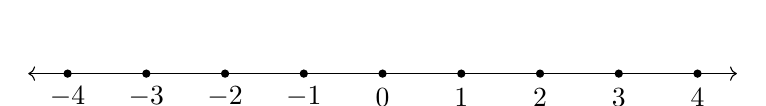
\begin{tikzpicture}
                \draw[<->] (-4.5, 0) -- (4.5, 0);
    
                \foreach \x in {-4, -3, -2, -1, 0, 1, 2, 3, 4}
                    \fill (\x, 0) circle (1.5pt);

                \foreach \x in {-4, -3, -2, -1, 0, 1, 2, 3, 4}
                    \node at (\x, -0.3) {$\x$};
            \end{tikzpicture}
        \end{center}
        Moreover, note that $-1 = e^{-2\pi i/2}$ and $i = e^{2\pi i/4}$. Then the fibers of these elements are just the integral differences of $1/2, 1/4$, and $2/3$ respectively, since $4\pi i/3 = 2/3(2\pi i)$:
        \begin{align*}
            \phi\inv(-1) & = \frac 12 + \z = \set*{\left.\frac 12 + n~\right|~n \in \z} \\
            \phi\inv(i) & = \frac 14 + \z = \set*{\left.\frac 14 + n~\right|~n \in \z} \\
            \phi\inv(e^{4\pi i/3}) & = \frac 23 + \z = \set*{\left.\frac 23 + n~\right|~n \in \z} \qh
        \end{align*}
    \end{sol}
    \item Repeat the preceding exercise with the map $\varphi$ replaced by the map $\varphi : r \mapsto e^{4\pi i r}$.
    \begin{sol}
        The kernel of $\phi$ is $\frac12\z$, or
        \begin{center}
            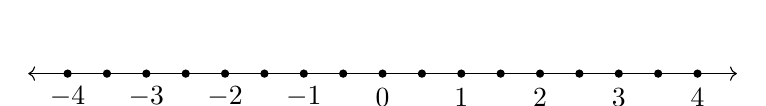
\begin{tikzpicture}
                \draw[<->] (-4.5, 0) -- (4.5, 0);
    
                \foreach \x in {-4, -3.5, -3, -2.5, -2, -1.5, -1, -0.5, 0, 0.5, 1, 1.5, 2, 2.5, 3, 3.5, 4}
                    \fill (\x, 0) circle (1.5pt);

                \foreach \x in {-4, -3, -2, -1, 0, 1, 2, 3, 4}
                    \node at (\x, -0.3) {$\x$};
            \end{tikzpicture}
        \end{center}
        Moreover, the fibers are just all halved, so
        \begin{align*}
            \phi\inv(-1) & = \frac14 + \frac12 \z = \set*{\left.\frac14 + \frac n2~\right|~n \in \z} \\
            \phi\inv(-i) & = \frac18 + \frac12 \z = \set*{\left.\frac18 + \frac n2~\right|~n \in \z} \\
            \phi\inv(e^{4\pi i/3}) & = \frac13 + \frac12 \z = \set*{\left.\frac13 + \frac n2~\right|~n \in \z} \qh
        \end{align*}
    \end{sol}
    \item Consider the additive quotient group $\mathbb{Q}/\mathbb{Z}$.
    \begin{problems}
        \item Show that every coset of $\mathbb{Z}$ in $\mathbb{Q}$ contains exactly one representative $q \in \mathbb{Q}$ in the range $0 \le q < 1$.
        \item Show that every element of $\mathbb{Q}/\mathbb{Z}$ has finite order but that there are elements of arbitrarily large order.
        \item Show that $\mathbb{Q}/\mathbb{Z}$ is the torsion subgroup of $\mathbb{R}/\mathbb{Z}$ (cf.\ Exercise 6, Section 2.1).
        \item Prove that $\mathbb{Q}/\mathbb{Z}$ is isomorphic to the multiplicative group of roots of unity in $\mathbb{C}^\times$.
    \end{problems}
    \begin{solalph}
        \item Suppose $t \in \q$, and put $t = a/b$ in lowest terms. Then there exists unique $q, r$ such that $a = bq + r$, or that $t = q + r/b$, where $0 \leq r < 1$. Then $t + \z = q + r/b + \z = r/b + \z$. Since $r$ is unique, then $r/b$ is the representative of $t + \z$ such that $0 \leq r < 1$.
        \item Suppose $t = p/q \in \q$. Then $|t + \z| \leq q$, since $q(t + \z) = qt + \z = \z$ so that $t + \z$ has finite order. Moreover, $1/k + \z \in \q/\z$ has order $k$, but because $k \in \z$ can be made arbitrarily large, then $1/k + \z$ has arbitrarily large order.
        \item Note that $\q/\z \subseteq \tor(\r/\z)$ by the previous exercise, so it remains to show that cosets with irrational representatives do not have finite order. If $x + \z \in \r/\z$ with finite order $n$, and $x \in \r - \q$, then $n(x + \z) = nx + \z = \z$ implies that $nx \in \z$. But since $n \in \zp$, this implies that $x \in \z$, contradicting that it was irrational. Hence, $\tor(\r/\z) = \q/\z$.
        \item By Exercise 3.1.12, we have $\r/\z \cong S^1$. Note that $\tor(S^1)$ consists of $z \in \c\unt$ such that $z^n = 1$, which is precisely the set of roots of unity. Since $\tor(\r/\z) = \q/\z$, then $\q/\z$ is isomorphic to the set of roots of unity.
    \end{solalph}
    \item \label{ex3.1.15} Prove that a quotient of a divisible abelian group by any proper subgroup is also divisible. Deduce that $\mathbb{Q}/\mathbb{Z}$ is divisible (cf. \hyperref[ex2.4.19]{Exercise 2.4.19}).
    \begin{sol}
        Let $A$ be a divisible abelian group, and let $B$ be a proper subgroup of $A$. Pick $aB \in A/B$. Since $A$ is divisible, there exists $x \in A$ such that $x^n = a$ for $x \in A$ and $n \in \z$. Then $(xB)^n = x^nB = aB$ so that $A/B$ is divisible. Since $\q$ is divisible, and $\z < \q$ is proper, then $\q/\z$ is also divisible.
    \end{sol}
    \item Let $G$ be a group, let $N$ be a normal subgroup of $G$, and let $\bar{G} = G/N$. Prove that if $G = \langle x, y \rangle$ then $\bar{G} = \langle \bar{x}, \bar{y} \rangle$. Prove more generally that if $G = \langle S \rangle$ for any subset $S$ of $G$, then $\bar{G} = \langle \bar{S} \rangle$.
    \begin{sol}
        If $G = \gen S$, then for every $g \in G$, we have
        \[g = s_1s_2 \dots s_n \quad \text{where $s_i \in S$ for $1 \le i \le n$}\]
        Let $\bar S = \{sN \mid s \in S\}$. Then for any $\bar g \in \bar G$, we have
        \[gN = (s_1s_2 \ldots s_n)N = (s_1N)(s_2N) \dots (s_nN)\]
        so that $\bar g \in \bar S$. Hence, $\bar G = \gen{\bar S}$. The case where $\bar G = \gen{\bar x, \bar y}$ is similar, where every element $g \in G$ is of the form $g = w(x, y)$, where $w(x, y)$ denotes a word in $\gen{x, y}$.
    \end{sol}
    \item Let $G$ be the dihedral group of order $16$ (whose lattice appears in Section 2.5): $G = \langle r,s \mid r^8 = s^2 = 1,\ rs = sr^{-1} \rangle$, and let $\bar{G} = G/\langle r^4 \rangle$ be the quotient of $G$ by the subgroup generated by $r^4$ (this subgroup is the center of $G$, hence is normal).
    \begin{problems}
        \item Show that the order of $\bar{G}$ is $8$.
        \item Exhibit each element of $\bar{G}$ in the form $\bar{s}^a \bar{r}^b$, for some integers $a$ and $b$.
        \item Find the order of each of the elements of $\bar{G}$ exhibited in (b).
        \item Write each of the following elements of $\bar{G}$ in the form $\bar{s}^a \bar{r}^b$, for some integers $a$ and $b$ as in (b): $\bar{rs}$, $\bar{sr^{-2}s}$, $\bar{s^{-1}r^{-1}sr}$.
        \item Prove that $\bar{H} = \langle \bar{s}, \bar{r}^2 \rangle$ is a normal subgroup of $\bar{G}$ and $\bar{H}$ is isomorphic to the Klein $4$-group. Describe the isomorphism type of the complete preimage of $\bar{H}$ in $G$.
        \item Find the center of $\bar G$ and describe the isomorphism type of $\bar G/Z(\bar G)$.
    \end{problems}
    \begin{solalph}
        \item Since $\gen{r^4} = \set{1, r^4}$, each coset in $\bar G$ has 2 elements and partitions $G$ into 8 sets. Hence, $\abs{\bar G} = 8$.
        \item The elements of $\bar G$ are
        \begin{align*}
            \bar 1 & = \{1, r^4\}, & \bar{s} & = \{s, sr^4\} \\
            \bar r & = \{r, r^5\}, & \bar{sr} & = \{sr, sr^5\} \\
            \bar r^2 & = \{r^2, r^6\}, & \bar{sr^2} & = \{sr^2, sr^6\} \\
            \bar r^3 & = \{r^3, r^7\}, & \bar{sr^3} & = \{sr^3, sr^7\}
        \end{align*}
        \item The orders of the elements of $\bar G$ are
        \[
        \begin{array}{c|c|c|c|c|c|c|c|c}
            \bar x & \bar 1 & \bar r & \bar r^2 & \bar r^3 & \bar s & \bar{sr} & \bar{sr^2} & \bar{sr^3} \\
            \hline
            \abs x & 1 & 4 & 2 & 4 & 2 & 2 & 2 & 2
        \end{array}
        \]
        \item $\bar{rs} = \bar{sr^3}, \bar{sr^{-2}s} = \bar r^2, \bar{s\inv r\inv sr} = \bar r^2$.
        \item We first note that $\bar H = \{1, \bar r^2, \bar s, \bar{sr^2}\}$. To show that $\bar H \nsub \bar G$, we simplify the process by noting that elements of $\bar G$ are of the form $\bar r^k$ or $\bar{sr^k}$. If an element is of the former, we have
        \begin{align*}
            \bar{r^kr^2r^{-k}} = \bar r^2 \in \bar H \\
            \bar{r^ksr^{-k}} = \bar{s(r^2)^{-k}} \in \bar H
        \end{align*}
        If it is of the latter, then
        \begin{align*}
            \bar{(sr^k)r^2(r^{-k}s)} = \bar{r^{-2}} \in H \\
            \bar{(sr^k)s(r^{-k}s)} = \bar{s(r^2)^k} \in H
        \end{align*}
        where $\bar{sr^k}\inv = \bar{r^{-k}s}$. The above calculations show that for every $\bar g \in \bar G$, then $\bar{gr^2g\inv}, \bar{gsg\inv} \in H$ so that $\bar{gHg\inv} = \bar H$, hence $\bar H \nsub \bar G$. Moreover, it is easy to see that every element of $\bar H$ is of order 2 so that $\bar H \cong V_4$.

        Let $\pi : G \to \bar G$ be the natural projection of $G$ onto $\bar G$. Then $\pi\inv(\bar H)$ is the complete preimage of $\bar H$, or the set of elements that map to a coset in $\bar H$. Using part (b), we see that
        \[\pi\inv(\bar H) = \{1, r^2, r^4, r^6, s, sr^2, sr^4, sr^6\}\]
        Note that $|\pi\inv(\bar H)| = 8$, and the elements of $\bar H$ satisfy the relations $(r^2)^4 = s^2 = 1$. Then the mapping $\phi : D_8 \to \pi\inv(\bar H)$ given by $\phi(r) = r^2$ and $\phi(s) = s$ extends to a homomorphism that is clearly surjective. Then $\phi$ is an isomorphism, and $\pi\inv(\bar H) \cong D_8$.
        \item From the previous exercise, we have that $\bar G = \gen{\bar r, \bar s}$. Since $\bar r^2$ commutes with both $\bar r$ and $\bar s$, then $\bar r^2 \in Z(\bar G)$. However, $\bar{rs} \neq \bar{sr}$ and $\bar{r^3s} \neq \bar{sr^3}$. Additionally, none of $\bar{sr}, \bar{sr^2}$, nor $\bar{sr^3}$ commute with $\bar r$ so that $Z(\bar G) = \{\bar 1, \bar r^2\}$. The elements of $\widehat G = \bar G/Z(\bar G)$ are as follows:
        \begin{align*}
            \hat 1 & = \{\bar 1, \bar r^2\} & \hat s & = \{\bar s, \bar{sr^2}\} \\
            \hat r & = \{\bar r, \bar r^3\} & \widehat{sr} & = \{\bar{sr}, \bar{sr^3}\}
        \end{align*}
        One can see that each nonidentity element of $\widehat G$ has order 2 so that $\widehat G \cong V_4$.
    \end{solalph}
    \item Let $G$ be the quasidihedral group of order $16$ (whose lattice was computed in Exercise 11 of Section 2.5): $G = \langle \sigma,\tau \mid \sigma^8 = \tau^2 = 1,\ \sigma\tau = \tau\sigma^3 \rangle$, and let $\bar{G} = G/\langle \sigma^4 \rangle$ be the quotient of $G$ by the subgroup generated by $\sigma^4$ (this subgroup is the center of $G$, hence is normal).
    \begin{problems}
        \item Show that the order of $\bar{G}$ is $8$.
        \item Exhibit each element of $\bar{G}$ in the form $\bar{\tau}^a \bar{\sigma}^b$, for some integers $a$ and $b$.
        \item Find the order of each of the elements of $\bar{G}$ exhibited in (b).
        \item Write each of the following elements of $\bar{G}$ in the form $\bar{\tau}^a \bar{\sigma}^b$, for some integers $a$ and $b$ as in (b): $\bar{\sigma\tau}$, $\bar{\tau\sigma^{-2}\tau}$, $\bar{\tau^{-1}\sigma^{-1}\tau\sigma}$.
        \item Prove that $\bar{G} \cong D_8$.
    \end{problems}
    \begin{solalph}
        \item $\gen{\sigma^4}$ has 2 elements, so each coset has 2 elements which subsequently split $G$ into 8 cosets. Hence, $\abs{\bar G} = 8$.
        \item The elements are
        \begin{align*}
            \bar 1 & = \{1, \sigma^4\} & \bar\tau & = \{\tau, \tau\sigma^4\} \\
            \bar\sigma & = \{\sigma, \sigma^5\} & \bar{\tau\sigma} & = \{\tau\sigma, \tau\sigma^5\} \\
            \bar\sigma^2 & = \{\sigma^2, \sigma^6\} & \bar{\tau\sigma^2} & = \{\tau\sigma^2, \tau\sigma^6\} \\
            \bar\sigma^3 & = \{\sigma^3, \sigma^7\} & \bar{\tau\sigma^3} & = \{\tau\sigma^3, \tau\sigma^7\}
        \end{align*}
        \item The orders are
        \[
        \begin{array}{c|c|c|c|c|c|c|c|c}
            \bar x & \bar 1 & \bar\sigma & \bar\sigma^2 & \bar\sigma^3 & \bar\tau & \bar{\tau\sigma} & \bar{\tau\sigma^2} & \bar{\tau\sigma^3} \\
            \hline
            \abs{\bar x} & 1 & 4 & 2 & 4 & 2 & 2 & 2 & 2
        \end{array}
        \]
        \item $\bar{\sigma\tau} = \bar{\tau\sigma^3}, \bar{\tau\sigma^{-2}\tau} = \bar\sigma^2, \bar{\tau\inv\sigma\inv\tau\sigma} = \bar\sigma^2$.
        \item Note that $\bar\sigma^4 = \bar\tau^2 = \bar 1$, and $\bar{\sigma\tau} = \bar{\tau\sigma^3} = \bar{\tau\sigma^7} = \bar{\tau\sigma}$ so that $\bar G$ satisfies the same relations in $D_8$. Then the mapping $\phi : \bar G \to D_8$ given by $\phi(\bar\sigma) = r$ and $\phi(\bar\tau) = s$ extends to a surjective homomorphism, hence $\bar G \cong D_8$.
    \end{solalph}
    \item Let $G$ be the modular group of order $16$ (whose lattice was computed in Exercise 14 of Section 2.5): $G = \langle u,v \mid u^2 = v^8 = 1,\ vu = uv^5 \rangle$, and let $\bar{G} = G/\langle v^4 \rangle$ be the quotient of $G$ by the subgroup generated by $v^4$ (this subgroup is contained in the center of $G$, hence is normal).
    \begin{problems}
        \item Show that the order of $\bar{G}$ is $8$.
        \item Exhibit each element of $\bar{G}$ in the form $\bar{u}^a \bar{v}^b$, for some integers $a$ and $b$.
        \item Find the order of each of the elements of $\bar{G}$ exhibited in (b).
        \item Write each of the following elements of $\bar{G}$ in the form $\bar{u}^a \bar{v}^b$, for some integers $a$ and $b$ as in (b): $\bar{vu}$, $\bar{uv^{-2}u}$, $\bar{u^{-1}v^{-1}uv}$.
        \item Prove that $\bar{G}$ is abelian and is isomorphic to $Z_2 \times Z_4$.
    \end{problems}
    \begin{solalph}
        \item $\gen{v^4}$ has 2 elements, so each coset has 2 elements. Then $G$ is split into 8 cosets, hence $\abs{\bar G} = 8$.
        \item The elements are
        \begin{align*}
            \bar 1 & = \{1, v^4\} & \bar u & = \{u, uv^4\} \\
            \bar v & = \set{v, v^5} & \bar{uv} & = \set{uv, uv^5} \\
            \bar v^2 & = \set{v^2, v^6} & \bar{uv^2} & = \set{uv^2, uv^6} \\
            \bar v^3 & = \set{v^3, v^7} & \bar{uv^3} & = \set{uv^3, uv^7}
        \end{align*}
        \item The orders are
        \[
        \begin{array}{c|c|c|c|c|c|c|c|c}
            \bar x & \bar 1 & \bar v & \bar v^2 & \bar v^3 & \bar u & \bar{uv} & \bar{uv^2} & \bar{uv^3} \\
            \hline
            \abs{\bar x} & 1 & 4 & 2 & 4 & 2 & 2 & 2 & 2
        \end{array}
        \]
        \item $\bar{vu} = \bar{uv^5}, \bar{uv^{-2}u} = \bar u^2, \bar{u\inv v\inv uv} = \bar 1$.
        \item Since $\bar{vu} = \bar{uv^5} = \bar{uv}$, $\bar G$ is abelian. Moreover, using the presentation of $Z_2 \times Z_4$ in \hyperref[ex2.5.12]{Section 2.5, Exercise 12}, we see that $\bar u^2 = \bar v^4 = 1$ so that $\bar G$ satisfies the same relations. Then $\phi : \bar G \to Z_2 \times Z_4$ given by $\phi(\bar u) = a$ and $\phi(\bar v) = b$ is a surjective homomorphism, hence $\bar G \cong Z_2 \times Z_4$.
    \end{solalph}
    \item Let $G = \mathbb{Z}/24\mathbb{Z}$ and let $\wt{G} = G/\langle \bar{12} \rangle$, where for each integer $a$ we simplify notation by writing $\wt{\bar a}$ as $\wt{a}$.
    \begin{problems}
        \item Show that $\wt{G} = \{ \wt{0}, \wt{1}, \ldots, \wt{11} \}$.
        \item Find the order of each element of $\bar{G}$.
        \item Prove that $\wt{G} \cong \mathbb{Z}/12\mathbb{Z}$ (thus $(\mathbb{Z}/24\mathbb{Z})/(12\mathbb{Z}/24\mathbb{Z}) \cong \mathbb{Z}/12\mathbb{Z}$, just as if we inverted and canceled the $24\mathbb{Z}$'s).
    \end{problems}
    \begin{solalph}
        \item Note that for some $\wt x \in \wt G$, we have $\wt x = \bar x\gen{12} = \{\bar x, \bar{x + 12}\}$. It follows that $x = 0, 1, 2, \dots, 11$ produces distinct cosets.
        \item The orders are
        \[
        \begin{array}{c|c|c|c|c|c|c|c|c|c|c|c|c}
            \wt x & \wt 0 & \wt 1 & \wt 2 & \wt 3 & \wt 4 & \wt 5 & \wt 6 & \wt 7 & \wt 8 & \wt 9 & \wt{10} & \wt{11} \\
            \hline
            \abs{\wt x} & 1 & 12 & 6 & 4 & 3 & 12 & 2 & 12 & 3 & 4 & 6 & 12
        \end{array}
        \]
        \item Define the mapping $\phi : \wt G \to \intmod[12]$ given by $\phi(\wt x) = \bar x$. This map is trivially a bijection, and for any $\wt x, \wt y \in \wt G$, then
        \[\phi(\wt x + \wt y) = \phi(\wt{x + y}) = \bar{x + y} = \bar x + \bar y = \phi(\wt x) + \phi(\wt y)\]
        so that $\phi$ is a homomorphism. Then $\wt G \cong \intmod[12]$.
    \end{solalph}
    \item Let $G = Z_4 \times Z_4$ be given in terms of the following generators and relations:
    \[G = \gen{x, y \mid x^4 = y^4 = 1, xy = yx}\]
    Let $\bar G = G/\gen{x^2y^2}$ (note that every subgroup of the abelian group $G$ is normal).
    \begin{problems}
        \item Show that the order of $\bar G$ is 8.
        \item Exhibit each element of $\bar G$ in the form $\bar x^a \bar y^b$ for some integers $a$ and $b$.
        \item Find the order of each elements of $\bar G$ exhibited in (b).
        \item Prove that $\bar G \cong Z_4 \times Z_2$.
    \end{problems}
    \begin{solalph}
        \item Note that $(x^2y^2)^2 = x^4y^4 = 1$ so that $\gen{x^2y^2} = \{1, x^2y^2\}$. Then each coset of $\bar G$ has 2 elements, hence its order is 8.
        \item Noting that $\bar x^2 \bar y^2 = \bar 1$ in $\bar G$, we have $\bar x^2 = \bar y^2$. Then we have the elements
        \begin{align*}
            \bar 1 & = \{1, x^2y^2\} & \bar y & = \{y, x^2y^3\} \\
            \bar x & = \{x, x^3y^2\} & \bar{xy} & = \{xy, x^3y^3\} \\
            \bar x^2 & = \{x^2, y^2\} & \bar{x^2y} & = \{x^2y, y^3\} \\
            \bar x^3 & = \{x^3, xy^2\} & \bar{x^3y} & = \{x^3y, xy^3\}
        \end{align*}
        \item The orders are
        \[
        \begin{array}{c|c|c|c|c|c|c|c|c}
            \bar g & \bar 1 & \bar x & \bar x^2 & \bar x^3 & \bar y & \bar{xy} & \bar{x^2y} & \bar{x^3y} \\
            \hline
            \abs{\bar g} & 1 & 4 & 2 & 4 & 4 & 2 & 4 & 2
        \end{array}
        \]
        \item Using the presentation of $Z_2 \times Z_4$ in \hyperref[ex2.5.12]{Section 2.5, Exercise 12}, and noting that $\bar{xy}^2 = \bar x^4 = 1$ then the mapping $\phi : Z_2 \times Z_4 \to \bar G$ given by
        \[\phi(a) = \bar{xy}, \quad \phi(b) = \bar x\]
        extends to a unique homomorphism. Now suppose $\phi(a^sb^t) = \phi(a^ub^v)$. Then $\bar{xy}^s\bar x^t = \bar{xy}^u\bar x^v$. Since $\gen{\bar{xy}} \cap \gen{\bar x}$ is trivial, then $\bar{xy}^{s - u} = \bar x^{v - t}$ imply that both quantities must be one. Then $\bar{xy}^s = \bar{xy}^u$ and $\bar x^v = \bar x^t$. Then $s \equiv u \bmod 2$ and $v \equiv t \bmod 4$, so that $a^sb^t = a^ub^t$ since $\abs a = 2$ and $\abs b = 4$. Then $\phi$ is injective. Because $\abs{Z_2 \times Z_4} = \abs{\bar G} = 8$, then $\phi$ is an isomorphism, hence $\bar G \cong Z_2 \times Z_4 \cong Z_4 \times Z_2$.
    \end{solalph}
    \item
    \begin{problems}
        \item Prove that if $H$ and $K$ are normal subgroups of a group $G$ then their intersection $H \cap K$ is also a normal subgroup of $G$.
        \item Prove that the intersection of an arbitrary nonempty collection of normal subgroups of a group is a normal subgroup (do not assume the collection is countable).
    \end{problems}
    \begin{solalph}
        \item Observe that $H \cap K \leq G$ since $H \leq G$ and $K \leq G$. Let $g \in G$ and $x \in H \cap K$. Since $H \nsub G$ and $K \nsub G$, then $gxg\inv \in H$ and $gxg\inv \in K$, hence $gxg\inv \in H \cap K$. Then $g(H \cap K)g\inv \subseteq H \cap K$. By Theorem 3.6, then $H \cap K \nsub G$.
        \item Let $G$ be a group and $I$ be a nonempty set of indices, possibly not countable. Consider the collection of subgroups $\{N_i \mid i \in I\}$ of $G$, where $N_i \nsub G$ for every $i \in I$. Consider their intersection
        \[N = \bigcap_{i \in I} N_i\]
        Since $N \leq G$, what remains to be shown is that $gNg\inv \subseteq N$ for some $g \in G$. To that end, let $n \in N$. Then $gng\inv \in N_i$ for each $i \in I$ because $N_i \nsub G$. It follows that $gng\inv \in N$ so that $gNg\inv \subseteq N$.
    \end{solalph}
    \item Prove that the join (cf. Section 2.5) of any nonempty collection of normal subgroups of a group is a normal subgroup.
    \begin{sol}
        Let $G$ be a group and $I$ be a nonempty set of indices. Let $\{N_i \mid i \in I\}$ be a collection of normal subgroups of $G$, and let $N = \gen{N_i \mid i \in I}$ be the join of the collection. Let $g \in G$ and $n \in N$. Then
        \[n = n_1n_2 \dots n_k \quad \text{where $n_i \in N_i$ for some $i \in I$}\]
        Since $N_i \nsub G$, then $gn_ig\inv \in N_i$ for each $1 \leq i \leq k$. Then
        \[gng\inv = g(n_1n_2 \ldots n_k)g\inv = (gn_1g\inv)(gn_2g\inv) \cdots (gn_kg\inv)\]
        Because $gng\inv$ is written as a product of elements where each one belongs to some $N_i$, it follows that it is in the join $N$, hence $gNg\inv \subseteq N$. Then $N \nsub G$.
    \end{sol}
    \item Prove that if $N \nsub G$ and $H$ is any subgroup of $G$ then $N \cap H \nsub H$.
    \begin{sol}
        We know $N \cap H \leq G$, so pick $h \in H$ and $x \in N \cap H$. Since $N \nsub G$, then $hxh\inv \in N$. Since $H \leq G$, then $hxh\inv \in H$ so that $hxh\inv \in N \cap H$. Then $N \cap H \nsub H$.
    \end{sol}
    \item 
    \begin{problems}
        \item Prove that a subgroup $N$ of $G$ is normal if and only if $gNg^{-1} \subseteq N$ for all $g \in G$.
        \item Let $G = \gl_2(\mathbb{Q})$, let $N$ be the subgroup of upper triangular matrices with integer entries and $1$'s on the diagonal, and let $g$ be the diagonal matrix with entries $2,1$. Show that $gNg^{-1} \subseteq N$ but $g$ does not normalize $N$.
    \end{problems}
    \begin{solalph}
        \item \rightimp If $N \nsub G$, then $gNg\inv \subseteq N$ holds true for all $g \in G$.
        \down\noindent
        \leftimp Suppose $gNg\inv \subseteq N$ for every $g \in G$, and let $n \in N$. To show that $N \subseteq gNg\inv$, note for some $g \in G$, then $g\inv Ng \subseteq N$ so that $g\inv ng \in N$. It follows that $n = g(g\inv ng)g\inv \in gNg\inv$ so that $N = gNg\inv$, hence $N \nsub G$.
        \item Let
        \[n = 
        \begin{pmatrix}
            1 & x \\
            0 & 1
        \end{pmatrix} \in N\]
        where $x \in \z$. Then
        \[gng\inv = 
        \begin{pmatrix}
            2 & 0 \\
            0 & 1
        \end{pmatrix}
        \begin{pmatrix}
            1 & x \\
            0 & 1
        \end{pmatrix}
        \begin{pmatrix}
            1/2 & 0 \\
            0 & 1
        \end{pmatrix} = 
        \begin{pmatrix}
            1 & 2x \\
            0 & 1
        \end{pmatrix} \in N\]
        since $2x \in \z$. Notice that the upper right entry of $gng\inv$ for any $n \in N$ will be even, so any matrix with an odd integer in the upper right entry will have no such $n \in N$ such that $gng\inv$ is that matrix.
    \end{solalph}
    \item Let $a,b \in G$.
    \begin{problems}
        \item Prove that the conjugate of the product of $a$ and $b$ is the product of the conjugate of $a$ and the conjugate of $b$. Prove that the order of $a$ and the order of any conjugate of $a$ are the same.
        \item Prove that the conjugate of $a^{-1}$ is the inverse of the conjugate of $a$.
        \item Let $N = \langle S \rangle$ for some subset $S$ of $G$. Prove that $N \nsub G$ if $gSg^{-1} \subseteq N$ for all $g \in G$.
        \item Deduce that if $N$ is the cyclic group $\langle x \rangle$, then $N$ is normal in $G$ if and only if for each $g \in G$, $gxg^{-1} = x^k$ for some $k \in \mathbb{Z}$.
        \item Let $n$ be a positive integer. Prove that the subgroup $N$ of $G$ generated by all the elements of $G$ of order $n$ is a normal subgroup of $G$.
    \end{problems}
    \begin{solalph}
        \item Note that $g(ab)g\inv = (gag\inv)(gbg\inv)$. The second result follows by \hyperref[ex1.1.22]{Exercise 1.1.22}.
        \item For any $g \in G$, then
        \[(ga\inv g\inv)(gag\inv) = ga\inv (g\inv g) ag\inv = g(a\inv a)g\inv = gg\inv = 1\]
        so that $(gag\inv)\inv = ga\inv g\inv$.
        \item If $S$ is empty, then $N$ is trivial, so the result follows. Suppose $S$ is not empty, and pick $n \in N$. Because $N = \gen S$, then we have $n = s_1s_2 \ldots s_k$, where $s_i \in S$ for each $i = 1, 2, \ldots, k$. Since 
        \[gng\inv = (gs_1g\inv)(gs_2g\inv) \cdots (gs_kg\inv)\]
        for every $g \in G$, and $gSg\inv \subseteq N$, then the right hand side is also in $N$, hence $gNg\inv \subseteq N$ so that $N \nsub G$.
        \item \rightimp Immediate from the definition of a normal subgroup.
        
        \noindent \leftimp Put $S = \set x$ and use the previous part.
        \item Let $S = \set{g \in G \mid \abs g = n}$, and put $N = \gen S$. If $S$ is empty, then $N$ is trivial, hence is normal. If $S$ is nonempty, note that part (a) shows that for any $g \in G$ and $s \in S$, then $\abs{gsg\inv} = \abs s = n$ so that $gsg\inv \in S \subseteq N$. Then $gSg\inv \subseteq N$, hence $N \nsub G$ by part (c).
    \end{solalph}
    \item Let $N$ be a \textit{finite} subgroup of a group $G$. Show that $gNg^{-1} \subseteq N$ if and only if $gNg^{-1} = N$. Deduce that $N_G(N) = \{ g \in G \mid gNg^{-1} \subseteq N \}$.
    \begin{sol}
        \rightimp Suppose $gNg\inv \subseteq N$. For any $g \in G$, define a mapping $\phi : N \to gNg\inv$ given by $\phi(n) = gng\inv$. If $\phi(m) = \phi(n)$, then $gmg\inv = gng\inv$ so that $\phi$ is injective by cancellation. Moreover, if $m \in gNg\inv$, there exists $n \in N$ such that $m = gng\inv = \phi(n)$ so that $\phi$ is surjective. It follows that $\phi$ is a bijection, and $\abs N = \abs{gNg\inv}$. Since $gNg\inv \subseteq N$, and $N$ is finite, it follows that $gNg\inv = N$.

        \noindent \leftimp Immediate.

        Note that $N_G(N) = \set{g \in G \mid gNg\inv = N}$. We may replace the condition that $gNg\inv = N$ with $gNg\inv \subseteq N$ by the implication showed above.
    \end{sol}
    \item Let $N$ be a \textit{finite} subgroup of a group $G$ and assume $N = \langle S \rangle$ for some subset $S$ of $G$. Prove that an element $g \in G$ normalizes $N$ if and only if $gSg^{-1} \subseteq N$.
    \begin{sol}
        \rightimp Immediate, since $gSg\inv \subseteq gNg\inv = N$ because $g \in N_G(N)$.

        \noindent \leftimp If $S$ is empty, then $N$ is trivial hence the conclusion follows. Suppose $S$ is not empty, and pick $n \in N$. Then $n = s_1s_2 \dots s_k$, where $s_i \in S$ for every $i = 1, 2, \ldots, k$. Then $gng\inv = gs_1g\inv gs_2g\inv \ldots gs_kg\inv \in N$ because $gs_ig\inv \in gSg\inv \subseteq N$. Then $gNg\inv \subseteq N$, and by the previous exercise, $g \in N_G(N)$. 
    \end{sol}
    \item Let $N$ be a \textit{finite} subgroup of $G$ and suppose $G = \langle T \rangle$ and $N = \langle S \rangle$ for some subsets $S$ and $T$ of $G$. Prove that $N$ is normal in $G$ if and only if $tSt^{-1} \subseteq N$ for all $t \in T$.
    \begin{sol}
        \rightimp Immediate, since $gNg\inv = N$ for every $g \in G$, so $tSt\inv \subseteq N$.

        \noindent \leftimp Suppose $S$ and $T$ are nonempty subsets of $G$, and let $g \in G$. Since $g \in \gen T$, then $g = t_1t_2 \dots t_k$, where $t_i \in T$ for each $i = 1, 2, \ldots, k$. Since we need to show this for every $g \in G$, we must proceed by inducting on the word length of $g \in \gen T$. To that end, $t_1St_1\inv \subseteq N$, so the base case is satisfied. Assume now that $gSg\inv \subseteq N$ when $g$ is some $k$-length word made up of elements from $T$. Consider the $k+1$-length word $g = t_1t_2 \ldots t_kt_{k + 1}$, where $t_i \in T$ for each $i = 1, 2, \ldots, k + 1$. For notation, set $\hat t = t_1t_2 \ldots t_k$ so that $g = \hat tt_{k + 1}$. The induction assumption shows that $\hat tS\hat t\inv \subseteq N$. For any $s \in S$, then 
        \[gsg\inv = \hat tt_{k + 1}st_{k + 1}\inv h\inv = \hat t(t_{k + 1}st_{k + 1}\inv)\hat t\inv\]
        where $t_{k + 1}st_{k + 1}\inv \in N$ because $tSt\inv \subseteq N$ for every $t \in T$. Since $N = \gen S$, then we may set $t_{k + 1}st_{k + 1}\inv = s_1s_2 \ldots s_m$, where $s_i \in S$ for every $i = 1, 2, \ldots, m$. Then
        \[\hat t(t_{k + 1}st_{k + 1}\inv)\hat t\inv = (\hat ts_1\hat t\inv)(\hat ts_2 \hat t\inv) \cdots (\hat ts_m \hat t\inv) \in N\]
        Hence, $gsg\inv \in N$ so that $gSg\inv \subseteq N$. Induction shows that this is true for every $g \in G$, and by finiteness of $N$, we use the result from the previous exercise to conclude that $N \nsub G$.
    \end{sol}
    \item Let $N \le G$ and let $g \in G$. Prove that $gN = Ng$ if and only if $g \in N_G(N)$.
    \begin{sol}
        \rightimp Suppose $gN = Ng$. For some $n \in N$, there exists $n' \in N$ such that $ng = gn'$, or $n = gn'g\inv$. Then $n \in gNg\inv$ so that $N \subseteq gNg\inv$. Moreover, if $n \in N$, then for some $n' \in N$ we have $gn = n'g$ so that $gng\inv = n'$, hence $gNg\inv \subseteq N$, hence $g \in N_G(N)$.
        
        \noindent \leftimp Suppose $g \in N_G(N)$ and $n \in N$. Since $n \in gNg\inv$, there exists $n' \in N$ such that $n = gn'g\inv$ so that $ng = gn'$, hence $n \in gN$, and $Ng \subseteq gN$. By symmetry, we have $gN \subseteq Ng$, hence $gN = Ng$.
    \end{sol}
    \item Prove that if $H \le G$ and $N$ is a normal subgroup of $H$ then $H \le N_G(N)$. Deduce that $N_G(N)$ is the largest subgroup of $G$ in which $N$ is normal (i.e. is the join of all subgroups $H$ for which $N \nsub H$).
    \begin{sol}
        If $h \in H$, then $hNh\inv = N$ because $N \nsub H$, hence $h \in N_G(N)$. Because $N_G(N) \leq G$, then $H \subseteq N_G(N)$ implies $H \leq N_G(N)$. Moreover, since every subgroup such that $N$ is normal in is a subgroup of $N_G(N)$, then $N_G(N)$ is the largest subgroup in which $N$ is normal.
    \end{sol}
    \item Prove that every subgroup of $Q_8$ is normal. For each subgroup find the isomorphism type of its corresponding quotient. [You may use the lattice of subgroups for $Q_8$ in Section 2.5.]
    \begin{sol}
        By the lattice, the subgroups of $Q_8$ are 1, $\gen{-1}, \gen i, \gen j, \gen k$, and $Q_8$. It is clear that $Q_8/1 \cong Q_8$, and $Q_8/Q_8 \cong 1$. Now, the lattice shows that $\gen i, \gen j$, and $\gen k$ are all maximal subgroups, so their normalizers must either be themselves, or $Q_8$. Since $j\gen i (-j) = \gen i$, then $j \in N_{Q_8}(\gen i)$ so that $N_{Q_8}(\gen i) = Q_8$. We may similarly argue that $N_{Q_8}(\gen j) = N_{Q_8}(\gen k) = Q_8$. Moreover, $Z(Q_8) = \gen{-1}$, and every center of a group is normal. It follows that every subgroup of $Q_8$ is normal.
        
        Let us first examine $Q_8/\gen{-1} = \{\bar 1, \bar i, \bar j, \bar k\}$. Since $\bar i^2 = \bar{-1} = \bar 1$, then $\abs{\bar i} = 2$. We can argue that $\abs{\bar j} = \abs{\bar k} = 2$ so that $Q_8/\gen{-1} \cong V_4$. The quotient group $Q_8/\gen i = \{\bar 1, \bar j\}$ has order 2 so $Q_8/\gen i \cong Z_2$. By symmetry, $Q_8/\gen j \cong Q_8/\gen k \cong Z_2$.
    \end{sol}
    \item Find all normal subgroups of $D_8$ and for each of these find the isomorphism type of its corresponding quotient. [You may use the lattice of subgroups for $D_8$ in Section 2.5.]
    \begin{sol}
        Again, $D_8/1 \cong D_8$ and $D_8/D_8 \cong 1$. Examining the three maximal subgroups $\gen{s, r^2}, \gen r$, and $\gen{rs, r^2}$. observe the following:
        \begin{align*}
            r\gen{s, r^2}r\inv & = \{1, sr^2. r^2, s\} = \gen{s, r^2} \\
            s\gen r s\inv & = \{1, r^3, r^2, r\} = \gen r \\
            r\gen{rs, r^2}r\inv & = \{1, sr, r^2, sr^3\} = \gen{rs, r^2}
        \end{align*}
        then the normalizers of each subgroup contain $r$ and $s$, hence $N_{D_8}(\gen{s, r^2}) = N_{D_8}(\gen r) = N_{D_8}(\gen{rs, r^2}) = Q_8$. Moreover, each of these maximal subgroups are of order 4, which means their corresponding quotient groups will have order 2, hence $Q_8/\gen{s, r^2} \cong Q_8/\gen r \cong Q_8/\gen{rs, r^2} \cong Z_2$.

        Now we examine $\gen{r^2} = Z(D_8)$ so it is clearly normal. Then $D_8/\gen{r^2} = \{\bar 1, \bar r, \bar s, \bar{sr}\}$. Note that the nonidentity elements have order 2, and so $D_8/\gen{r^2} \cong V_4$.

        For the remaining subgroups of order 2, observe that
        \begin{align*}
            r\gen{s}r\inv & = \{1, sr^2\} \neq \gen s \\
            r\gen{sr}r\inv & = \{1, rs\} \neq \gen{sr} \\
            r\gen{sr^2}r\inv & = \{1, s\} \neq \gen{sr^2} \\
            r\gen{sr^3}r\inv & = \{1, sr\} \neq \gen{sr^3}
        \end{align*}
        so that none of the subgroups of order 2 contain $r$, hence none of them are normal.
    \end{sol}
    \item Let $D_{2n} = \langle r,s \mid r^n = s^2 = 1,\ rs = sr^{-1} \rangle$ be the usual presentation of the dihedral group of order $2n$ and let $k$ be a positive integer dividing $n$.
    \begin{problems}
        \item Prove that $\langle r^k \rangle$ is a normal subgroup of $D_{2n}$.
        \item Prove that $D_{2n}/\langle r^k \rangle \cong D_{2k}$.
    \end{problems}
    \begin{solalph}
        \item Observe that $\gen{r^k} = \{1, r^k, r^{2k}, \ldots, r^{n - k}\}$. It is clear that $r\gen{r^k}r\inv = \gen{r^k}$, and observe that $sr^ks\inv = r^{-k} = r^{n - k}$ so that $s\gen{r^k}s\inv = \gen{r^k}$. Since $r, s \in N_{D_{2n}}(\gen{r^k})$, then $\gen{r^k} \nsub D_{2n}$.
        \item Consider $D_{2n}/\gen{r^k}$. Since $k \mid n$, then the order of $\gen{r^k}$ is $n/k$, and the number of cosets in the quotient group is $2n/(n/k) = 2k$. Now consider the cosets $\bar r$ and $\bar s$:
        \[\bar r = \{r, r^{k + 1}, r^{2k + 1}, \ldots, r^{n - k + 1}\} \quad \text{and} \quad \bar s = \{s, sr^k, sr^{2k}, \ldots, sr^{n - k}\}\]
        It is clear that $\bar s \neq \bar 1$, and $\bar s^2 = \bar 1$ so that $\abs{\bar s} = 2$. Moreover, $\bar r^k = \bar 1$, hence $\abs{\bar r} \leq k$. However, note that $\bar r^i = \bar 1$ when $i \mid k$ so that $\abs{\bar r} = k$. This clearly satisfies the relations for $D_{2k}$, hence $D_{2n}/\gen{r^k} \cong D_{2k}$. 
    \end{solalph}
    \item \label{ex3.1.35} Prove that $\speclin_n(F) \nsub \gl_n(F)$ and describe the isomorphism type of the quotient group (cf. Exercise 9, Section 2.1).
    \begin{sol}
        We know that $\speclin_n(F) \leq \gl_n(F)$, so we just need to show that $A \speclin_n(F) A\inv = \speclin_n(F)$ for all $A \in \gl_n(F)$. To that end, note that for any $S \in \speclin_n(F)$ and $X \in \gl_n(F)$, then $\det(XSX\inv) = \det(X)\det(S)\det(X\inv) = 1$, hence $X\speclin_n(F)X\inv \subseteq \speclin_n(F)$, and $\speclin_n(F) \nsub \gl_n(F)$.

        Recall that when a subgroup is normal, it is actually the kernel of some homomorphism. Observe that every element of $\speclin_n(F)$ has determinant 1, so if we consider the mapping $A \mapsto \det(A)$ for some $A \in \gl_n(F)$, then the kernel of this homomorphism is clearly $\speclin_n(F)$. We may then consider the mapping $\phi : \gl_n(F)/\speclin_n(F) \to F\unt$ given by $\phi(\bar X) = \det(X)$.

        We now show that this mapping is well defined. Suppose $\bar A = \bar B$ for some $\bar A, \bar B \in \gl_n(F)/\speclin_n(F)$. Recall that the elements of $\bar A$ are of the form $AS$ for $A \in \gl_n(F)$ and some $S \in \speclin_n(F)$. Since $\bar A = \bar B$, then for $AS \in \bar A$ there exists $S' \in \speclin_n(F)$ such that $AS = BS_0$. Then
        \[\phi(\bar A) = \det(A) = \det(AS) = \det(BS') = \det(B) = \phi(\bar B)\]
        so that $\phi$ is well defined.
        
        To show that $\phi$ is injective, suppose $\phi(\bar A) = \phi(\bar B)$. Then $\det(A) = \det(B)$. Pick some $AS \in \bar A$, where $S \in \speclin_n(F)$. Observe that $B\inv AS \in \speclin_n(F)$, since $\det(B\inv AS) = \det(B\inv)\det(A)\det(S) = \det(A)\inv\det(A)\det(S) = 1$, hence $B\inv AS = S'$ for some $S' \in \speclin_n(F)$. Then $AS = BS'$, and $AS \in \bar B$ so that $\bar A \subseteq \bar B$. A similar argument shows that $\bar B \subseteq \bar A$ so that $\bar A = \bar B$, and $\phi$ is injective. Moreover, for some $f \in F\unt$, then $\det(fI_n) = f\det(I_n) = f$ so that $\phi$ is surjective. Lastly, for $\bar A, \bar B \in \speclin_n(F)$, then 
        \[\phi(\bar{AB}) = \det(AB) = \det(A)\det(B) = \phi(\bar A)\phi(\bar B)\]
        so that $\phi$ is a homomorphism. Then $\phi$ is a bijective homomorphism, and $\gl_n(F)/\speclin_n(F) \cong F\unt$. 
    \end{sol}
    \item \label{ex3.1.36} Prove that if $G/Z(G)$ is cyclic then $G$ is abelian. [If $G/Z(G)$ is cyclic with generator $xZ(G)$, show that every element of $G$ can be written in the form $x^a z$ for some integer $a \in \mathbb{Z}$ and some element $z \in Z(G)$.]
    \begin{sol}
        Suppose $G/Z(G) = \gen{xZ(G)}$ for some $x \in G$. Then cosets are of the form $x^aZ(G)$ for some $a \in \z$. Suppose $g, h \in G$. Since both $g$ and $h$ belong to some coset in $G/Z(G)$, then $g = x^mz$ and $h = x^nz'$ for some $m, n \in \z$ and $z, z' \in Z(G)$. Then
        \[ab = (x^mz)(x^nz') = (x^nz')(x^mz) = ba\]
        so that $G$ is abelian.
    \end{sol}
    \item Let $A$ and $B$ be groups. Show that $\{(a,1) \mid a \in A\}$ is a normal subgroup of $A \times B$ and the quotient of $A \times B$ by this subgroup is isomorphic to $B$.
    \begin{sol}
        Let $C$ be the the given set. It is clear that $C \leq A \times B$. Suppose $(a, b) \in A \times B$. Then for any $(a', 1) \in C$, we have
        \[(a, b)(a', 1)(a, b)\inv = (aa'a\inv, b1b\inv) = (aa'a\inv, 1) \in C\]
        so that $C \nsub A \times B$.

        Consider the mapping $\phi : A \times B/C \to B$ given by $\phi(\bar{(a, b)}) = b$. To show that this is well-defined, suppose $\bar{(a, b)} = \bar{(a', b')}$. Then $(a, b)C = (a', b')C$, which implies that $C = (a\inv, b\inv)(a', b')C$, or that $(a\inv a', b\inv b') \in C$. Then $b\inv b' = 1$, or $b = b'$ so that $\phi$ is well-defined.

        Now suppose $\phi(\bar{(a, b)}) = \phi(\bar{(a', b')})$. Then $b = b'$ so that $(a, b)C = (a', b')C$, hence $\phi$ is injective. Moreover, $\phi(\bar{(1, b)}) = b$ so that $\phi$ is surjective. Lastly, for $\bar{(a, b)}, \bar{(a', b')} \in A \times B/C$, then 
        \[\phi(\bar{(a, b)}\bar{(a', b')}) = \phi(\bar{(aa', bb')}) = bb' = \phi(\bar{(a, b)})\phi(\bar{(a', b')})\]
        so that $\phi$ is a bijective homomorphism. Hence, $A \times B/C \cong B$.
    \end{sol}
    \item Let $A$ be an abelian group and let $D$ be the (diagonal) subgroup $\{(a,a) \mid a \in A\}$ of $A \times A$. Prove that $D$ is a normal subgroup of $A \times A$ and $(A \times A)/D \cong A$.
    \begin{sol}
        Since $A$ is abelian, then $A \times A$ is abelian, hence any subgroup is normal so that $D \nsub A \times A$.

        Now consider two cosets $\bar{(a_1, a_2)}, \bar{(a_3, a_4)} \in (A \times A)/D$. Then $\bar{(a_1, a_2)} = \bar{(a_3, a_4)}$ when we have $(a_1, a_2)\inv(a_3, a_4) \in D$, which implies that $a_1\inv a_3 = a_2\inv a_4$, or $a_3a_4\inv = a_1a_2\inv$. We can construct a well-defined, injective homomorphism $\phi : (A \times A)/D \to A$ given by $\phi(\bar{(a, b)}) = ab\inv$. Moreover, this is surective, since $\phi(\bar{(a, 1)}) = a$ for any $a \in A$. Lastly, it is a homomorphism, because
        \begin{align*}
            \phi(\bar{(a_1, b_1)(a_2, b_2)}) & = \phi(\bar{(a_1a_2, b_1b_2)}) \\
            & = (a_1a_2)(b_1b_2)\inv \\
            & = (a_1b_1\inv)(a_2b_2\inv) \\
            & = \phi(\bar{(a_1, b_1)})\phi(\bar{(a_2, b_2)})
        \end{align*}
        Hence, $\phi$ is a bijective homomorphism, and $(A \times A)/D \cong A$.
    \end{sol}
    \item Suppose $A$ is the non-abelian group $S_3$ and $D$ is the diagonal subgroup $\{(a,a) \mid a \in A\}$ of $A \times A$. Prove that $D$ is not normal in $A \times A$.
    \begin{sol}
        Let $\alpha, \beta \in S_3$, where $\alpha = 1$ and $\beta = (1\ 2\ 3)$ so that $\alpha\inv = \alpha$ and $\beta\inv \neq \beta$. For $\gamma = (1\ 2) \in S_3$, consider $\alpha\gamma\alpha\inv$ and $\beta\gamma\beta\inv$. Observe that $\alpha\gamma\alpha\inv = \gamma$, while $\beta\gamma\beta\inv = (1\ 2\ 3)(1\ 2)(3\ 2\ 1) = (2\ 3) \neq (1\ 2) = \gamma$. Then $(\alpha, \beta)(\gamma, \gamma)(\alpha\inv, \beta\inv) = (\gamma, (2\ 3))$, hence $D$ is not a normal subgroup of $S_3 \times S_3$.
    \end{sol}
    \item \label{ex3.1.40}Let $G$ be a group, let $N$ be a normal subgroup of $G$ and let $\bar{G} = G/N$. Prove that $\bar{x}$ and $\bar{y}$ commute in $\bar{G}$ if and only if $x^{-1}y^{-1}xy \in N$. (The element $x^{-1}y^{-1}xy$ is called the \textit{commutator} of $x$ and $y$ and is denoted by $[x,y]$.)
    \begin{sol}
        \rightimp Suppose $\bar{xy} = \bar{yx}$. Then $xyN = yxN$. Then there exists $n, n' \in N$ such that $xyn = yxn'$, or $x\inv y\inv xy = n'n\inv$ so that $x\inv y\inv xy \in N$.

        \noindent \leftimp Suppose $x\inv y\inv xy\in N$. Then there is $n \in N$ such that $x\inv y\inv xy = n$, or $xy = yxn$. Then $a \in xyN$ if and only if $a = xyn'$ for some $n' \in N$ if and only if $a = yxnn'$ if and only if $a \in yxN$. Hence, $\bar{xy} = \bar{yx}$.
    \end{sol}
    \item Let $G$ be a group. Prove that $N = \langle x^{-1}y^{-1}xy \mid x,y \in G \rangle$ is a normal subgroup of $G$ and $G/N$ is abelian ($N$ is called the \textit{commutator} subgroup of $G$).
    \begin{sol}
        Let $g \in G$ and $x\inv y\inv xy \in N$. Then 
        \[g(x\inv y\inv xy)g\inv = (gx\inv g\inv)(g y\inv g\inv)(gxg\inv)(gyg\inv) = (gxg\inv)\inv(gyg\inv)\inv(gxg\inv)(gyg\inv) \in N\]
        so that $g[x, y]g\inv = [gxg\inv, gyg\inv] \in N$. Then $gNg\inv \subseteq N$, hence $N \nsub G$.
        
        $G/N$ is abelian, since the previous exercise shows that $\bar x$ and $\bar y$ in $G/N$ commute when $[x, y] \in N$.
    \end{sol}
    \item Assume both $H$ and $K$ are normal subgroups of $G$ with $H \cap K = 1$. Prove that $xy = yx$ for all $x \in H$ and $y \in K$. [Show $x^{-1}y^{-1}xy \in H \cap K$.]
    \begin{sol}
        Let $x \in H$ and $y \in K$. Since $H \nsub G$, then $y\inv xy \in H$, hence $[x, y] \in H$. Since $K \nsub G$, then $x\inv y\inv x\in K$, hence $[x, y] \in K$. Then $[x, y] \in H \cap K = 1$ so that $[x, y] = 1$. It follows that $x\inv y\inv xy = 1$, or $xy = yx$.
    \end{sol}
    \item Assume $\mathcal{P} = \{A_i \mid i \in I\}$ is any partition of $G$ with the property that $\mathcal{P}$ is a group under the ``quotient operation'' defined as follows: to compute the product of $A_i$ with $A_j$ take any element $a_i$ of $A_i$ and any element $a_j$ of $A_j$ and let $A_iA_j$ be the element of $\mathcal{P}$ containing $a_ia_j$ (this operation is assumed to be well defined). Prove that the element of $\mathcal{P}$ that contains the identity of $G$ is a normal subgroup of $G$ and the elements of $\mathcal{P}$ are the cosets of this subgroup (so $\mathcal{P}$ is just a quotient group of $G$ in the usual sense).
    \begin{sol}
        For any $g \in G$, let $\bar g \in \pp$ be the element such that $g \in \bar g$. Now, $\bar 1 \in \pp$ is the set such that $1 \in \bar 1$ so that $\bar 1$ is nonempty. Moreover, for any $g, h \in \bar 1$, we have $\bar{gh} = \bar g \cdot \bar h = \bar 1 \cdot \bar 1 = \bar 1$ so that $\bar 1$ is closed under the operation. Lastly, we have that $\bar{g\inv} = \bar{g\inv} \cdot \bar 1 = \bar{g\inv} \cdot \bar g = \bar{g\inv g} = \bar 1$ so that $\bar 1$ is closed under inverses, hence $\bar 1 \leq G$.
        
        To show that $\bar 1 \nsub G$, let $g \in G$ and $x \in \bar 1$. Then $\bar{gxg\inv} = \bar g \cdot \bar x \cdot \bar{g\inv} = \bar g \cdot \bar 1 \cdot \bar{g\inv} = \bar{gg\inv} = \bar 1$, hence $gxg\inv \in \bar 1$ so that $\bar 1 \nsub G$.

        Consider some $g\bar 1 \in G/\bar 1$, and let $\bar g \in \pp$. For some $gy \in g\bar 1$ where $y \in \bar 1$, then $\bar{gy} = \bar g \cdot \bar y = \bar g \cdot \bar 1 = \bar g$ so that $gy \in \bar g$, hence $g \bar 1 \subseteq \bar g$. If $x \in \bar g$, then $\bar x = \bar g$ so that $\bar{g\inv x} = \bar{g\inv g} = \bar 1$, hence $g\inv x \in \bar 1$. Then $x = gg\inv x = g(g\inv x) \in g\bar 1$, hence $\bar g \subseteq g\bar 1$. It follows that $\bar g = g\bar 1$.
    \end{sol}
\end{problems}

\newpage

\subsection{More on Cosets and Lagrange's Theorem}

Let $G$ be a group.

\begin{problems}
    \item Which of the following are permissible orders for subgroups of a group of order 120: 1, 2, 5, 7, 9, 15, 60, 240? For each permissible order give the corresponding index.
    \begin{sol}
        Only 1, 2, 5, 9, 15, and 60 are permissible orders for subgroups of a group of order 120. The corresponding indices are 120, 60, 24, 12, 8, and 2, respectively.
    \end{sol}
    \item Prove that the lattice of subgroups of $S_3$ in Section 2.5 is correct (i.e., prove that it contains all subgroups of $S_3$ and that their pairwise joins and intersections are correctly drawn).
    \begin{sol}
        Since $|S_3| = 6$, then Lagrange's Theorem shows that non-trivial subgroups are of order 2 and 3. Clearly, none of the cyclic subgroups of order 2 can be contained in $\gen{(1\ 2\ 3)}$ since it has order 3. Moreover, $\gen{(1\ 2\ 3)} = \gen{(1\ 3\ 2)}$, hence all cyclic subgroups are accounted for, and the containment is correct.

        To prove that the subgroups of $S_3$ are only the cyclic subgroups in the lattice, suppose $S_3$ has a non-cyclic subgroup $H$ of order 3, and suppose $H = \gen{\sigma, \tau}$ for some $\sigma, \tau \in S_3$. We then have $H = \set{1, \sigma, \tau}$. Since $\abs\sigma$ divides $\abs H$, it must be that $\abs\sigma = 3$, hence $\sigma$ and $\sigma^2$ are distinct elements so that $\tau = \sigma^2$. Then $H = \gen\sigma$, contradicting it was non-cyclic. Hence, all proper subgroups of $S_3$ are cyclic, and the lattice is correct.
    \end{sol}
    \item Prove that the lattice of subgroups of $Q_8$ in Section 2.5 is correct.
    \begin{sol}
        Lagrange's Theorem shows that the possible orders of subgroups of $Q_8$ are 1, 2, 4, and 8. The only possible subgroup of order 2 is $\gen{-1}$ since it is the only element of order 2 in $Q_8$. The only subgroups of order 4 are $\gen i, \gen j$, ad $\gen k$ since every other nonidentity element has order 4 and are contained in one of these subgroups.

        Since $\gen{-1}$ is contained in each of $\gen i, \gen j$, and $\gen k$, and the subgroups of order 4 are maximal via Lagrange's, then the lattice is correct.
    \end{sol}
    \item Show that if $|G| = pq$ for some primes $p$ and $q$ (not necessarily distinct) then either $G$ is abelian or $Z(G) = 1$. [See \hyperref[ex3.1.36]{Exercise 3.1.36}.]
    \begin{sol}
        If $G$ is abelian, then we are done. Suppose $G$ is not abelian. It follows that $Z(G)$ is a proper subgroup of $G$, and by Lagrange's Theorem, the order of $Z(G)$ must be either 1, $p$, or $q$. Assume $Z(G)$ is not trivial, and without loss of generality, assume $|Z(G)| = p$. Since $Z(G) \nsub G$ as $Z(G)$ is abelian, then we may Lagrange's again to obtain $\abs{G/Z(G)} = \abs G/\abs{Z(G)} = q$, which is prime. Then $G/Z(G)$ is cyclic, so by \hyperref[ex3.1.36]{Exercise 3.1.36}, $G$ is abelian, a contradiction. Hence, $Z(G) = 1$.
    \end{sol}
    \item Let $H$ be a subgroup of $G$ and fix some element $g \in G$. 
    \begin{problems}
        \item Prove that $gH g^{-1}$ is a subgroup of $G$ of the same order as $H$.
        \item Deduce that if $n \in \mathbb{Z}^+$ and $H$ is the unique subgroup of $G$ of order $n$ then $H \nsub G$.
    \end{problems}
    \begin{solalph}
        \item Since $1 \in H$, then $g1g\inv = 1 \in gHg\inv$ so that $gHg\inv$ is nonempty. Now suppose $gxg\inv, gyg\inv \in gHg\inv$ for some $x, y \in H$. Then
        \[(gxg\inv)(gyg\inv)\inv = gxg\inv gy\inv g\inv = gxy\inv g\inv \in gHg\inv\]
        since $xy\inv \in H$. Hence, $gHg\inv \leq G$.

        Define a map $\phi : H \to gHg\inv$ by $\phi(h) = ghg\inv$. To show that this is a bijection, suppose $\phi(h_1) = \phi(h_2)$. Then $gh_1g\inv = gh_2g\inv$, hence $h_1 = h_2$ so that $\phi$ is injective. Moreover, for any $ghg\inv \in gHg\inv$, then $\phi(h) = ghg\inv$ so that $\phi$ is surjective. Hence, $\abs{gHg\inv} = \abs H$.
        \item Let $g \in G$. Since $H$ is the unique subgroup of $G$ of order $n$, then by part (a), $gHg\inv$ is a subgroup of $G$ of order $n$, hence $gHg\inv = H$. It follows that $H \nsub G$.
    \end{solalph}
    \item Let $H \leq G$ and let $g \in G$. Prove that if the right coset $Hg$ equals some left coset of $H$ in $G$ then it equals the left coset $gH$ and $g$ must be in $N_G(H)$.
    \begin{sol}
        Suppose $Hg = g'H$ for some $g' \in G$. Note that $g \in Hg$ so that $g \in g'H$. Then $Hg = g'H = gH$, hence $Hg = gH$, and $g \in N_G(H)$.
    \end{sol}
    \item Let $H \leq G$ and define a relation $\sim$ on $G$ by $a \sim b$ if and only if $b^{-1}a \in H$. Prove that $\sim$ is an equivalence relation and describe the equivalence class of each $a \in G$. Use this to prove Proposition 4.
    \begin{sol}
        Let $h \in H$. Since $h\inv h = 1 \in H$, then $h \sim h$ so that $\sim$ is reflexive. Suppose $g, h \in H$ such that $g \sim h$. Then $h\inv g \in H$, hence $g\inv h = (h\inv g)\inv \in H$ so that $h \sim g$ and $\sim$ is symmetric. Lastly, suppose $g, h, k \in G$ such that $g \sim h$ and $h \sim k$. Then $h\inv g \in H$ and $k\inv h \in H$, hence $(k\inv h)(h\inv g) = k\inv g \in H$ so that $g \sim k$ and $\sim$ is transitive. It follows that $\sim$ is an equivalence relation.

        The equivalence class of some $a \in G$ is given by $\set{b \in G \mid b\inv a \in H}$. Note that $b$ is in the equivalence class of $a$ when $b\inv a = h$ for some $h \in H$, hence $b = ah\inv$. The set becomes $\set{ah\inv \mid h \in H}$, which is the left coset of $H$ containing $a$. Since the equivalence classes partition $G$, then the left cosets of $H$ partition $G$, by Proposition 0.2, then the left cosets of $H$ in $G$ form a partition of $G$, proving Proposition 4.
    \end{sol}
    \item Prove that if $H$ and $K$ are finite subgroups of $G$ whose orders are relatively prime then $|H \cap K| = 1$.
    \begin{sol}
        Let $\abs H = m$ and $\abs K = n$ such that $(m, n) = 1$. Let $\ell = \abs{H \cap K}$. Since $H \cap K \leq H$ and $H \cap K \leq K$, then by Lagrange's Theorem, $\ell \mid m$ and $\ell \mid n$. It follows that $\ell \mid (m, n) = 1$, hence $\ell = 1$.
    \end{sol}
    \item This exercise outlines a proof of Cauchy's Theorem due to James McKay (\textit{Another proof of Cauchy's group theorem}, Amer. Math. Monthly, 66 (1959), p. 119). Let $G$ be a finite group and let $p$ be a prime dividing $|G|$. Let $\ss$ denote the set of $p$-tuples of elements of $G$ the product of whose coordinates is 1:
    \[\ss = \{(x_1, x_2, \ldots, x_p) \mid x_i \in G \text{ and } x_1x_2 \cdots x_p = 1\}\]
    \begin{problems}
        \item Show that $\ss$ has $|G|^{p-1}$ elements, hence has order divisible by $p$.
    \end{problems}
    Define the relation $\sim$ on $S$ by letting $\alpha \sim \beta$ if $\beta$ is a cyclic permutation of $\alpha$.
    \begin{problems}[resume]
        \item Show that a cyclic permutation of an element of $\ss$ is again an element of $\ss$.
        \item Prove that $\sim$ is an equivalence relation on $\ss$.
        \item Prove that an equivalence class contains a single element if and only if it is of the form $(x, x, \dots, x)$ with $x^p = 1$.
        \item Prove that every equivalence class has order 1 or $p$ (this uses the fact that $p$ is \textit{prime}). Deduce that $|G|^{p-1} = k + pd$, where $k$ is the number of classes of size 1 and $d$ is the number of classes of size $p$.
        \item Since $\{(1, 1, \dots, 1)\}$ is an equivalence class of size 1, conclude from (e) that there must be a nonidentity element $x \in G$ with $x^p = 1$, i.e., $G$ contains an element of order $p$. [Show $p \mid k$ and so $k > 1$.]
    \end{problems}
    \begin{solalph}
        \item Consider the $(p - 1)$-tuples of elements of $G$, and call this set $\ss'$. Clearly, $\ss'$ has $|G|^{p-1}$ elements. Now define a mapping $\phi : \ss' \to \ss$ by $\phi(x_1, x_2, \dots, x_{p-1}) = (x_1, x_2, \dots, x_{p-1}, (x_1x_2 \cdots x_{p-1})\inv)$. Now suppose $\phi(x_1, x_2, \dots, x_{p-1}) = \phi(y_1, y_2, \dots, y_{p-1})$. Then $(x_1, x_2, \dots, x_{p-1}, (x_1x_2 \cdots x_{p-1})\inv) = (y_1, y_2, \dots, y_{p-1}, (y_1y_2 \cdots y_{p-1})\inv)$ so that $x_i = y_i$ for all $1 \leq i \leq p - 1$, hence $\phi$ is injective. Moreover, this mapping is clearly surjective. It follows that $\abs\ss = \abs{\ss'} = |G|^{p-1}$.
        \item Let $\alpha = (x_1, x_2, \dots, x_p) \in \ss$. A cyclic permutation of $\alpha$ is some $\beta = (x_k, x_{k+1}, \dots, x_p, x_1, x_2, \dots, x_{k-1})$ for some $1 \leq k \leq p$ where the indices are taken modulo $p$. Observe that these consist of the same elements as $\alpha$, just in a different order, hence $x_k x_{k+1} \cdots x_p x_1 x_2 \cdots x_{k-1} = x_1 x_2 \cdots x_p = 1$, so that $\beta \in \ss$.
        \item Let $\alpha, \beta, \gamma \in \ss$. $\sim$ is clearly reflexive since $\alpha$ is a cyclic permutation of itself. 
        
        Suppose $\alpha \sim \beta$. Then $\beta$ is a cyclic permutation of $\alpha$, hence $\alpha$ is a cyclic permutation of $\beta$, so that $\beta \sim \alpha$ and $\sim$ is symmetric. 
        
        Lastly, suppose $\alpha \sim \beta$ and $\beta \sim \gamma$. Then $\beta$ is a cyclic permutation of $\alpha$, and $\gamma$ is a cyclic permutation of $\beta$, hence $\gamma$ is a cyclic permutation of $\alpha$ by taking the composition of the permutations, so that $\alpha \sim \gamma$ and $\sim$ is transitive. It follows that $\sim$ is an equivalence relation on $\ss$.
        \item \rightimp Let $[\alpha]$ denote the equivalence class that contains $\alpha$. If $[\alpha]$ contains a single element, then it must be that all cyclic permutations of $\alpha$ are equal, hence $\alpha = (x, x, \dots, x)$ for some $x \in G$. Since $\alpha \in \ss$, then $x^p = 1$.
        
        \noindent \leftimp Suppose $\alpha = (x, x, \dots, x)$ for some $x \in G$ such that $x^p = 1$. Then any cyclic permutation of $\alpha$ is equal to $\alpha$, hence $[\alpha]$ contains a single element.
        \item Let $\alpha = (x_1, x_2, \dots, x_p) \in \ss$ where the $x_i$ need not be distinct, and let $[\alpha]$ be the equivalence class containing $\alpha$. Suppose $[\alpha]$ has $n$ elements, and note that $x_i = x_j$ whenever $i + kn \equiv j \bmod p$ for some $k \in \z$ that represents the amount of cyclic shifts.
        
        There are two cases to discuss, either $n = p$ or $1 \leq n < p$. If $n = p$, then we are done. Suppose $1 \leq n < p$. Since $p$ is prime, then $(n, p) = 1$, hence there exists some $k \in \z$ such that $kn \equiv 1 \bmod p$. In particular, $i + kn \equiv i + 1 \equiv j \bmod p$ implies $x_{i + 1} = x_j$. It follows that $x_i = x_j$ for all $1 \leq i, j \leq p$, hence $\alpha = (x, x, \dots, x)$ for some $x \in G$. By part (c), $[\alpha]$ contains a single element.

        Since the equivalence classes partition $\ss$, let $k$ be the number of classes of size 1 and $d$ be the number of classes of size $p$. Then $\abs\ss = k + pd$, as desired.
        \item Because $p$ divides $\abs G$, then it divides $\abs\ss = |G|^{p-1}$. From part (d), we have $|G|^{p-1} = k + pd$, hence $p \mid k$ so that $k > 1$. Then there is at least one equivalence class of size 1 that is not $\{(1, 1, \dots, 1)\}$. By part (c), this equivalence class is of the form $(x, x, \dots, x)$ for some nonidentity $x \in G$ such that $x^p = 1$. It follows that $G$ contains an element of order $p$.
    \end{solalph}
    \item \label{ex3.2.10} Suppose $H$ and $K$ are subgroups of finite index in the (possibly infinite) group $G$ with $|G : H| = m$ and $|G : K| = n$. Prove that $\lcm(m, n) \leq |G : H \cap K| \leq mn$. Deduce that if $m$ and $n$ are relatively prime then $|G : H \cap K| = |G : H| \cdot |G : K|$.
    \begin{sol} 
        Let $|G : H \cap K| = \ell$. Consider the cosets $gH, gK$, and $g(H \cap K)$ for some $g \in G$. We wish to identify $g(H \cap K)$ in terms of $gH$ and $gK$. Note that $x \in g(H \cap K)$ implies that $g\inv x \in H \cap K$, hence $g\inv x \in H$ and $g\inv x \in K$, so that $x \in gH$ and $x \in gK$. It follows that $g(H \cap K) \subseteq gH \cap gK$. Now suppose $x \in gH \cap gK$. Then $x \in gH$ and $x \in gK$, hence $g\inv x \in H$ and $g\inv x \in K$, so that $g\inv x \in H \cap K$. It follows that $x \in g(H \cap K)$, hence $gH \cap gK \subseteq g(H \cap K)$. We conclude that $g(H \cap K) = gH \cap gK$.

        Note that the set of cosets of $H \cap K$ in $G$ partitions $G$ into $\ell$ parts, and each coset is the intersection of a coset of $H$ with a coset of $K$. Since there are $m$ cosets of $H$ and $n$ cosets of $K$, then there are at most $mn$ distinct intersections, hence $\ell \leq mn$. 

        We now show that $\ell$ is a multiple of $m$ (a similar argument can be done to show that it is a multiple of $n$). Let $x \in G$. Since the cosets of $H$ in $G$ partition $G$, then there exists a unique $g \in G$ such that $x \in gH$. Moreover, because $H \cap K \leq H$, then the cosets of $H \cap K$ in $H$ partition $H$ so that there exists a unique $h \in H$ such that $x \in gh(H \cap K)$. Pick another coset $h' \neq h$ of $H \cap K$ in $H$. Then $gh(H \cap K) \neq gh'(H \cap K)$ since if they were equal, then $(gh)\inv(gh') = h\inv h' \in H \cap K$, contradicting that $h$ and $h'$ are distinct cosets. It follows that for each coset of $H$ in $G$, there are $\abs{H : H \cap K}$ distinct cosets of $H \cap K$ in $G$. Since there are $m$ cosets of $H$ in $G$, then $\ell = m \abs{H : H \cap K}$, hence $m \mid \ell$. Similarly, $n \mid \ell$. Since $\ell$ is a multiple of both $m$ and $n$, then $\lcm(m, n) \mid \ell$, hence $\lcm(m, n) \leq \ell$, and we have the desired inequality $\lcm(m, n) \leq \ell \leq mn$.

        Lastly, if $(m, n) = 1$, then $\lcm(m, n) = mn$ so that $\ell = mn$.
    \end{sol}
    \item \label{ex3.2.11} Let $H \leq K \leq G$. Prove that $|G : H| = |G : K| \cdot |K : H|$. 
    \begin{sol}
        Note that cosets of $H$ are contained in cosets of $K$. If $H$ has infinite index in $K$ or if $K$ has infinite index in $G$, then $H$ has infinite index in $G$. The finite case follows in the proof of \hyperref[ex3.2.10]{Exercise 3.2.10}, where we showed that each coset of $K$ contains $\abs{K : H}$ distinct cosets of $H$. Since there are $\abs{G : K}$ distinct cosets of $K$ in $G$, then there are $\abs{G : K} \cdot \abs{K : H}$ distinct cosets of $H$ in $G$, hence $\abs{G : H} = \abs{G : K} \cdot \abs{K : H}$.
    \end{sol}
    \item Let $H \leq G$. Prove that the map $x \mapsto x^{-1}$ sends each left coset of $H$ in $G$ onto a right coset of $H$ and gives a bijection between the set of left cosets and the set of right cosets of $H$ in $G$ (hence the number of left cosets of $H$ in $G$ equals the number of right cosets).
    \begin{sol}
        Let $L$ be the set of left cosets of $H$ in $G$ and $R$ be the set of right cosets of $H$ in $G$. Define the map $\phi : L \to R$ be given by $\phi(xH) = Hx\inv$. Firstly, this map is well-defined: suppose $xH = yH$. Then $yx\inv \in H$, hence $(yx\inv)\inv = xy\inv \in H$, so that $Hx\inv = Hy\inv$. Note that the map $\psi : R \to L$ given by $\psi(Hx) = x\inv H$ is well-defined by a similar argument. It is clear that $\phi \circ \psi = 1$ and $\psi \circ \phi = 1$, hence $\psi = \phi\inv$ so that $\phi$ is a bijection. It follows that $\abs L = \abs R$.
    \end{sol}
    \item Fix any labelling of the vertices of a square and use this to identify $D_8$ as a subgroup of $S_4$. Prove that the elements of $D_8$ and $\gen{(123)}$ do not commute in $S_4$.
    \begin{sol}
        Let $D_8 = \{1, (1\ 2\ 3\ 4), (1\ 3)(2\ 4), (1\ 4\ 3\ 2), (2\ 4), (1\ 2)(3\ 4), (1\ 3), (1\ 4)(2\ 3)\}$ be the subgroup of $S_4$, where a square is labelled clockwise from 1 to 4. Note that $D_8$ is generated by $r = (1\ 2\ 3\ 4)$ and $s = (2\ 4)$. Then $(1\ 2\ 3)(1\ 2\ 3\ 4) = (1\ 3\ 4\ 2) \neq (1\ 4\ 3\ 2) = (1\ 2\ 3\ 4)(1\ 2\ 3)$, and $(1\ 2\ 3)(2\ 4) = (1\ 4\ 3) \neq (1\ 3\ 4) = (2\ 4)(1\ 2\ 3)$, so that the generators of $D_8$ do not commute with the generator of $\gen{(1\ 2\ 3)}$. It follows that the elements of $D_8$ and $\gen{(1\ 2\ 3)}$ do not commute in $S_4$.
    \end{sol}
    \item Prove that $S_4$ does not have a normal subgroup of order 8 or a normal subgroup of order 3.
    \begin{sol}
        Suppose $S_4$ has a normal subgroup $N$ of order 8. By Lagrange's then $N$ cannot contain any 3-cycle. Then elements of $N$ are comprised of at least the identity, 2-cycles, a product of 2 disjoint 2-cycles, or 4-cycles. Observe that $N$ cannot contain all 6 2-cycles of $S_4$ for otherwise $(1\ 2)(1\ 3) = (1\ 3\ 2) \in N$, a contradiction. It must be that there is some 2-cycle $\sigma \in S_4$ that is not in $N$. Since $N \nsub S_4$, then $N \gen\sigma \leq S_4$. Since $\sigma \not\in S_4$, then $N \cap \gen\sigma = 1$, hence $|N \gen\sigma| = 16$. This contradicts Lagrange's Theorem, hence $N$ cannot exist.

        If $S_4$ has a normal subgroup $M$ of order 3, then $M \cong Z_3$ which is cyclic. Since $S_4$ contains 4 distinct 3-cycles, we may pick another $\tau \in S_4$ such that $\tau \not\in M$, hence $M \cap \gen\tau = 1$. Because $M \nsub S_4$, we have $|M \gen\tau| = 9$, contradicting Lagrange's Theorem, hence $M$ cannot exist.
    \end{sol}
    \item Let $G = S_n$ and for fixed $i \in \{1, 2, \dots, n\}$ let $G_i$ be the stabilizer of $i$. Prove that $G_i \cong S_{n-1}$.
    \begin{sol}
        Observe that the elements of $G_i$ consists of permutations on the $\{1, 2, \ldots, n\} - \set i$ which has $n - 1$ elements. Then $G_i \cong S_{n - 1}$.
    \end{sol}
    \item Use Lagrange's Theorem in the multiplicative group $(\mathbb{Z}/p\mathbb{Z})^\times$ to prove \textit{Fermat's Little Theorem}: if $p$ is a prime then $a^p \equiv a \bmod p$ for all $a \in \z$.
    \begin{sol}
        Let $p$ be a prime. Note that $\units[p] = \{\bar 1, \bar 2, \ldots, \bar{p - 1}\}$. For any $a \in \z$, then we either have $a \mid p$ or $a \nmid p$. If $a \mid p$, then $a \equiv 0 \bmod p$, hence $a^p \equiv 0 \equiv a \bmod p$. If $a \nmid p$, then $\bar a \in \units[p]$. By Lagrange's Theorem and Corollary 3.9, $\abs{\bar a}$ divides $\abs{\units[p]} = p - 1$, hence $\bar a^{p - 1} = \bar 1$. Then $a^{p - 1} \equiv 1 \bmod p$, or $a^p \equiv a \bmod p$.
    \end{sol}
    \item Let $p$ be a prime and let $n$ be a positive integer. Find the order of $\bar p$ in $(\mathbb{Z}/(p^n - 1)\mathbb{Z})^\times$ and deduce that $n \mid \phi(p^n - 1)$ (here $\phi$ is Euler's function).
    \begin{sol}
        Since $p^n \equiv 1 \bmod (p^n - 1)$, then $\abs{\bar p} \leq n$. Suppose $d < n$ such that $p^d \equiv 1 \bmod (p^n - 1)$. Then $p^n - 1 \mid p^d - 1$ so that $p^n - 1 \leq p^d - 1$, a contradiction. It follows that $\abs{\bar p} = n$. By Lagrange's Theorem, $\abs{\bar p} = n$ divides $\abs{\units[p^n - 1]} = \phi(p^n - 1)$.
    \end{sol}
    \item Let $G$ be a finite group, let $H$ be a subgroup of $G$ and let $N \nsub G$. Prove that if $\abs H$ and $|G : N|$ are relatively prime then $H \leq N$.
    \begin{sol}
        Since $N \nsub G$, then $HN \leq G$. Moreover, $H \cap N \leq H$ so that $|H \cap N|$ divides $\abs H$. Then we have that $|G| = m|HN|$ and $|H| = n|H \cap N|$ for some $m, n \in \z$. By Corollary 13, we have that
        \[|HN| = \frac{\abs H \abs N}{|H \cap N|} \implies m|HN| = m\frac{n|H \cap N||N|}{|H \cap N|} \implies \frac{|G|}{|N|} = |G : N| = mn\]
        Since $(\abs H, |G : N|) = 1$, then $n = 1$ so that $\abs H = |H \cap N|$. It follows that $H = H \cap N$, hence $H \leq N$.
    \end{sol}
    \item Prove that if $N$ is a normal subgroup of the finite group $G$ and $(|N|, |G : N|) = 1$ then $N$ is the unique subgroup of $G$ of order $|N|$.
    \begin{sol}
        Let $M$ be a subgroup of $G$ with order $\abs N$. By the previous exercise, we have $M \leq N$, and since they have the same order, then $M = N$.
    \end{sol}
    \item If $A$ is an abelian group with $A \nsub G$ and $B$ is any subgroup of $G$ prove that $A \cap B \nsub AB$.
    \begin{sol}
        Suppose $y = abxb\inv a\inv \in ab(A \cap B)b\inv a\inv$ for some $x \in A \cap B$. Since $A \nsub G$, then $bxb\inv \in A$ so that $y = a(bxb\inv)a\inv = bxb\inv \in A$. Moreover, $bxb\inv \in B$ since $x \in B$, hence $y \in A \cap B$. It follows that $ab(A \cap B)b\inv a\inv \subseteq A \cap B$, so that $A \cap B \nsub AB$.
    \end{sol}
    \item Prove that $\mathbb{Q}$ has no proper subgroups of finite index. Deduce that $\mathbb{Q}/\mathbb{Z}$ has no proper subgroups of finite index. [Recall \hyperref[ex1.6.21]{Exercise 1.6.21} and \hyperref[ex3.1.15]{Exercise 3.1.15}.]
    \begin{sol}
        Suppose $\q$ has a proper subgroup $H$ such that $|\q : H|$ is some finite $n$. Recalling that $\q$ is divisible by \hyperref[ex2.4.19]{Exercise 2.4.19}, then $\q/H$ is also divisible by \hyperref[ex3.1.15]{Exercise 3.1.15}. However, $\q/H$ is a finite group of order $n$, hence it cannot be divisible unless it is trivial. It follows that $H = \q$, a contradiction. Therefore, $\q$ has no proper subgroups of finite index. Moreover, $\q/\z$ has no proper subgroup of finite index for the same reasoning.
    \end{sol}
    \item Use Lagrange's Theorem in the multiplicative group $(\mathbb{Z}/n\mathbb{Z})^\times$ to prove \textit{Euler's Theorem}: $a^{\varphi(n)} \equiv 1 \bmod n$ for every integer $a$ relatively prime to $n$, where $\varphi$ denotes Euler's $\varphi$-function.
    \begin{sol}
        Recall $\abs{\units} = \phi(n)$. Since $\bar a \in \units$, then $\abs{\bar a}$ divides $\phi(n)$, hence $a^{\phi(n)} \equiv 1 \bmod n$.
    \end{sol}
    \item Determine the last two digits of $3^{3^{100}}$. [Determine $3^{100} \bmod \phi(100)$ and use the previous exercise.]
    \begin{sol}
        Note that $100 = 2^2 \cdot 5^2$, then $\phi(100) = 2^1(2 - 1)5^1(5 - 1) = 40$. Since $3^4 \bmod 40 = 81 \bmod 40 \equiv 1 \bmod 40$, then $3^{100} \bmod 40 \equiv 1 \bmod 40$. It follows that $3^{100} = 1 + 40k = 1 + \phi(100)k$ for some $k \in \z$, hence
        \[3^{3^{100}} = 3^{1 + \phi(100)k} = 3 \cdot 3^{{\phi(100)}^k} \equiv 3 \cdot 1^k \bmod 100 = 3 \bmod 100\]
        so that the last two digits of $3^{3^{100}}$ are 03.
    \end{sol}
\end{problems}

\newpage

\subsection{The Isomorphism Theorems}

Let $G$ be a group.

\begin{problems}
    \item Let $F$ be a finite field of order $q$ and let $n \in \zp$. Prove that $|\gl_N(F) : \speclin_n(F)| = q - 1$. [See \hyperref[ex3.1.35]{Exercise 3.1.35}.]
    \begin{sol}
        In \hyperref[ex3.1.35]{Exercise 3.1.35}, we showed that $\speclin_n(F) \nsub \gl_n(F)$ and that $\gl_n(F)/\speclin_n(F) \cong F\unt$. Since $F$ is a finite field of order $q$, then $\abs{F\unt} = q - 1$. We then have that $|\gl_n(F) : \speclin_n(F)| = \abs{F\unt} = q - 1$.
    \end{sol}
    \item Prove all parts of the Lattice Isomorphism Theorem.
    \begin{sol}
        Let $\ac = \set{A \leq G \mid N \subseteq A}$ and $\bar{\ac} = \set{\bar A \leq \bar G}$. Define the map $\phi : \ac \to \bar{\ac}$ by $\phi(A) = \bar A = A/N$. Note that $\phi(A) \leq \bar G$ as follows: since $\bar 1 \in \bar A$, then $\bar A$ is nonempty. Moreover, for any $\bar a, \bar b \in \bar A$ where $a, b \in A$, then $ab\inv \in A$ implies $\bar a \bar b\inv = \overline{ab\inv} \in \bar A$, hence $\bar A \leq \bar G$. This also implies that $\phi$ is surjective, since for any $\bar A \in \bar{\ac}$, we know that the preimage of $\bar A$ under the natural projection homomorphism from $G$ to $G/N$ is some subgroup $A$ of $G$ containing $N$ such that $\phi(A) = \bar A$. Lastly, suppose $\phi(A) = \phi(B)$ for some $A, B \in \ac$. Then $\bar A = \bar B$ implies that for some $a \in A$, there is some $b \in B$ such that $\bar a = \bar b$, hence $aN = bN$ so that $b\inv a \in N \subseteq B$. It follows that $a = b(b\inv a) \in B$, hence $A \subseteq B$. A similar argument shows that $B \subseteq A$, hence $A = B$ so that $\phi$ is injective. Therefore, $\phi$ is a bijection.
        \begin{enumerate}
            \item \rightimp Suppose $A \leq B$ for $A, B \in \ac$, and suppose $\bar a \in \bar A$ for some $a \in A$. Since $A \leq B$, then $a \in B$ so that $\bar a \in \bar B$, hence $\bar A \leq \bar B$.
            
            \noindent \leftimp Suppose $\bar A \leq \bar B$ for $A, B \in \ac$, and suppose $a \in A$ for some $a \in A$. Then $\bar a \in \bar A$ so that $\bar a \in \bar B$, hence there is some $b \in B$ such that $\bar a = \bar b$. It follows that $aN = bN$ so that $b\inv a \in N \subseteq B$, hence $a = b(b\inv a) \in B$. Therefore, $A \leq B$.
            \item Consider a mapping $\psi : B/A \to \bar B / \bar A$ given by $\psi(bA) = \bar b \bar A$ for $b \in B$. To show $\psi$ is well-defined, suppose $b_1A = b_2A$ for some $b_1, b_2 \in B$. Then $b_2\inv b_1 \in A$, hence $\overline{b_2\inv b_1} \in \bar A$ so that $\bar b_1 \bar A = \bar b_2 \bar A$, hence $\psi(b_1A) = \psi(b_2A)$. It is clear that $\psi$ is a homomorphism, and it is surjective since for any $\bar b \bar A \in \bar B / \bar A$, there is some $b \in B$ such that $\psi(bA) = \bar b \bar A$. Finally, if $bA \in \ker\psi$, then $\psi(bA) = \bar A$ so that $\bar b \in \bar A$, hence $bN \in A/N$ or that $b \in A$. It follows that $\ker\psi = A/A = 1$, hence $\psi$ is an isomorphism. Therefore, $|B : A| = |B/A| = |\bar B / \bar A| = |\bar B : \bar A|$.
            \item $\bar x \in \bar{\gen{A, B}}$ if and only if $x = x_1x_2 \ldots x_n$ where $x_i \in A \cup B$ for each $1 \leq i \leq n$ if and only if $\bar x = \bar{x_1x_2} \ldots \bar{x_n}$ where $\bar{x_i} \in \bar A \cup \bar B$ for each $1 \leq i \leq n$ if and only if $\bar x \in \gen{\bar A, \bar B}$, hence $\bar{\gen{A, B}} = \gen{\bar A, \bar B}$.
            \item $\bar x \in \bar{A \cap B}$ if and only if $x \in A \cap B$ if and only if $x \in A$ and $x \in B$ if and only if $\bar x \in \bar A$ and $\bar x \in \bar B$ if and only if $\bar x \in \bar A \cap \bar B$, hence $\bar{A \cap B} = \bar A \cap \bar B$.
            \item \rightimp Suppose $A \nsub G$, and let $gN \in \bar G$. Then for any $\bar a \in \bar A$ where $a \in A$, we have that $gag\inv \in A$ so that $gNg\inv = gag\inv N \in \bar A$, hence $\bar A \nsub \bar G$.
            
            \noindent \leftimp Suppose $\bar A \nsub \bar G$, and let $g \in G$. Then for any $a \in A$, we have that $\bar g \bar a \bar g\inv \in \bar A$ so that $gag\inv N \in A/N$, hence $gag\inv \in A$, thus $A \nsub G$. \qh
        \end{enumerate}
    \end{sol}
    \item Prove that if $H$ is a normal subgroup of $G$ of prime index $p$ then for all $K \leq G$ either
    \begin{enumerate}
        \item[(i)] $K \leq H$ or
        \item[(ii)] $G = HK$ and $|K : K \cap H| = p$.
    \end{enumerate}
    \begin{sol}
        Since $H \nsub G$, then $N_G(H) = G$. Then $K \leq N_G(H)$, hence $KH \leq G$ by the Second Isomorphism Theorem. By Proposition 3.14, then $KH = HK$. Since we have $H \leq HK \leq G$, we may use \hyperref[ex3.2.11]{Exercise 3.2.11} to conclude that $|G : H| = |G : HK| \cdot |HK : H|$. Since $|G : H| = p$ is prime, we have that $|G : HK|$ is either 1 or $p$. If the former is true, then $G = HK$. If the latter is true, then $HK = H$, hence $K \leq H$. In particular, if the former is true, then $|HK : H| = p$, and we may use the Second Isomorphism Theorem to conclude that $HK/H \cong K/(K \cap H)$ so that $|K : K \cap H| = |HK : H| = p$.
    \end{sol}
    \item Let $C$ be a normal subgroup of the group $A$ and let $D$ be a normal subgroup of the group $B$. Prove that $(C \times D) \nsub (A \times B)$ and $(A \times B)/(C \times D) \cong (A/C) \times (B/D)$.
    \begin{sol}
        Consider the map $\phi : A \times B \to (A/C) \times (B/D)$ given by $\phi(a, b) = (aC, bD)$. This map is clearly well-defined and a homomorphism. Now suppose $\phi((a, b)) = (C, D)$. Then $aC = C$ and $bD = D$, hence $a \in C$ and $b \in D$, so that $(a, b) \in C \times D$, hence $\ker\phi \subseteq C \times D$. If $(c, d) \in C \times D$, then $\phi((c, d)) = (cC, dD) = (C, D)$, so that $C \times D \subseteq \ker\phi$. It follows that $\ker\phi = C \times D$, hence $C \times D \nsub A \times B$. Lastly, $\phi$ is clearly surjective since for any $(aC, bD) \in (A/C) \times (B/D)$, we have $\phi((a, b)) = (aC, bD)$. By the First Isomorphism Theorem, we have $(A \times B)/(C \times D) \cong (A/C) \times (B/D)$.
    \end{sol}
    \item Let $QD_{16} = \gen{\sigma, \tau}$ be the quasidihedral group of order 16 in \hyperref[ex2.5.11]{Exercise 2.5.11}. Prove that $\gen{\sigma^4}$ is normal in $QD_{16}$ and use the Lattice Isomorphism Theorem to draw the lattice of subgroups of $QD_{16}/\gen{\sigma^4}$. Which group of order 8 has the same lattice as this quotient? Use generators and relations for $QD_{16}$ to decide the isomorphism type of this group.
    \begin{sol}
        Note that $\tau\sigma^4\tau = \tau\tau\sigma^{12} = \sigma^4$, hence $\gen{\sigma^4} \nsub QD_{16}$. By the Lattice Isomorphism Theorem, we may draw the following diagram:
        \begin{center}
            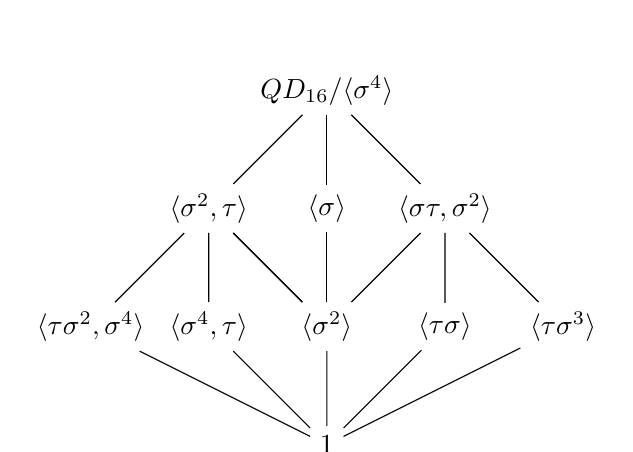
\begin{tikzpicture}[scale=1.5]
                \node (d8) at (0, 0) {$QD_{16}/\gen{\sigma^4}$};
                
                \node (sr2) at (-1, -1) {$\bar{\gen{\sigma^2, \tau}}$};
                \node (r) at (0, -1) {$\bar{\gen\sigma}$};
                \node (rsr2) at (1, -1) {${\bar{\gen{\sigma\tau, \sigma^2}}}$};

                \node (s) at (-2, -2) {$\bar{\gen{\tau\sigma^2, \sigma^4}}$};
                \node (r2s) at (-1, -2) {$\bar{\gen{\sigma^4, \tau}}$};
                \node (r2) at (0, -2) {$\bar{\gen{\sigma^2}}$};
                \node (rs) at (1, -2) {$\bar{\gen{\tau\sigma}}$};
                \node (r3s) at (2, -2) {$\bar{\gen{\tau\sigma^3}}$};
                
                \node (1) at (0, -3) {1};

                \draw (1) -- (s) -- (sr2) -- (d8);
                \draw (1) -- (r2s) -- (sr2);
                \draw (1) -- (r2) -- (sr2);
                \draw (1) -- (rs) -- (rsr2) -- (d8);
                \draw (1) -- (r3s) -- (rsr2);
                \draw (r2) -- (r) -- (d8);
                \draw (r2) -- (sr2);
                \draw (r2) -- (rsr2);
            \end{tikzpicture}
        \end{center}
        Moreover, $\bar{\sigma^4} = \bar{\tau^2} = \bar 1$ and $\bar{\tau\sigma} = \bar{\sigma^3\tau} = \bar{\sigma\inv\tau}$, then the generators $\bar\sigma$ and $\bar\tau$ satisfy the relations as $r$ and $s$ do in $D_8$, hence $QD_{16}/\gen{\sigma^4} \cong D_8$.
    \end{sol}
    \item Let $M = \gen{u, v}$ be the modular group of order 16 in \hyperref[ex2.5.14]{Exercise 2.5.14}. Prove that $\gen{v^4}$ is normal in $M$ and use the Lattice Isomorphism Theorem to draw the lattice of subgroups of $M/\gen{v^4}$. Which group of order 8 has the same lattice as this quotient? Use generators and relations for $M$ to decide the isomorphism type of this group.
    \begin{sol}
        Note that $uv^4u = uuv^{20} = v^4$, hence $\gen{v^4} \nsub M$. By the Lattice Isomorphism Theorem, we may draw the following diagram:
        \begin{center}
            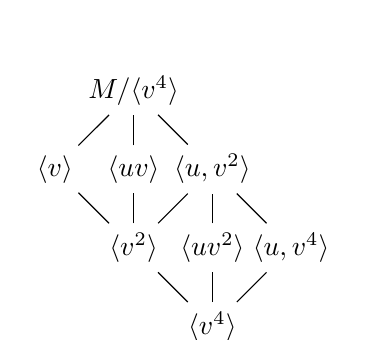
\begin{tikzpicture}[every node/.style=on grid]
                \node (G) {$M/\gen{v^4}$};

                \node (y) [below left=of G] {$\bar{\gen v}$};
                \node (xy) [below=of G] {$\bar{\gen{uv}}$};
                \node (x y2) [below right=of G] {$\bar{\gen{u, v^2}}$};

                \node (y2) [below right=of y] {$\bar{\gen{v^2}}$};
                \node (xy2) [below=of x y2] {$\bar{\gen{uv^2}}$};
                \node (x y4) [below right=of x y2] {$\bar{\gen{u, v^4}}$};

                \node (y4) [below right=of y2] {$\bar{\gen{v^4}}$};

                \draw (y4) -- (y2) -- (y) -- (G);
                \draw (y4) -- (x y4) -- (x y2) -- (G);
                \draw (y4) -- (xy2) -- (x y2);
                \draw (y2) -- (xy) -- (G);
                \draw (y2) -- (x y2);
            \end{tikzpicture}
        \end{center}
        Moreover, $\bar{v^4} = \bar{u^2} = \bar 1$ and $\bar{vu} = \bar{uv^5} = \bar{uv}$ so that the generators of $M/\gen{v^4}$ satisfy the relations as $a$ and $b$ do in $Z_2 \times Z_4$, whose presentation is given in \hyperref[ex2.5.12]{Exercise 2.5.12}. Then $M/\gen{v^4} \cong Z_2 \times Z_4$.
    \end{sol}
    \item Let $M$ and $N$ be normal subgroups of $G$ such that $G = MN$. Prove that $G/(M \cap N) \cong (G/M) \times (G/N)$. [Draw the lattice.]
    \begin{sol}
        The lattice is given as the following, where double lines represent the quotient group $G/(M \cap N)$:
        \begin{center}
            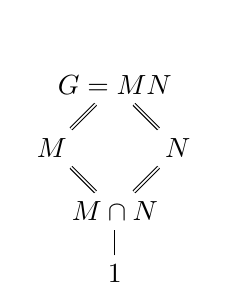
\begin{tikzpicture}[scale=0.8]
                \node (MN) at (0, 0) {$G = MN$};
                \node (M) at (-1, -1) {$M$};
                \node (N) at (1, -1) {$N$};
                \node (MnN) at (0, -2) {$M \cap N$};
                \node (1) at (0, -3) {1};

                \draw (1) -- (MnN);
                \draw [double] (MnN) -- (M) -- (MN);
                \draw [double] (MnN) -- (N) -- (MN);
            \end{tikzpicture}
        \end{center}
        Now consider the mapping $\phi : G \to (G/M) \times (G/N)$ given by $\phi(g) = (gM, gN)$. This is clearly a homomorphism with $\ker\phi = M \cap N$. Now let $(gM, hN) \in (G/M) \times (G/N)$. Since $G = MN$, there exist $m, m' \in M$ and $n, n' \in N$ such that $g = mn$ and $h = m'n'$. Then $\phi(mn') = (mnM, mn'N) = (gM, hN)$, hence $\phi$ is surjective. By the First Isomorphism Theorem, we have $G/(M \cap N) \cong \phi(G) = (G/M) \times (G/N)$.
    \end{sol}
    \item Let $p$ be a prime and let $G$ be the group of $p$-power roots  of $1$ in $\c$ (cf. \hyperref[ex2.4.18]{Exercise 2.4.18}). Prove that the map $z \mapsto z^p$ is a surjective homomorphism. Deduce that $G$ is isomorphic to a proper quotient of itself.
    \begin{sol}
        Let $\phi(z) = z^p$ be the map. For any $z, w \in G$, then $\phi(zw) = (zw)^p = z^p w^p = \phi(z)\phi(w)$, hence $\phi$ is a homomorphism. Moreover, for any $y \in G$, there is some $n \in \zp$ such that $y^{p^n} = 1$. Then let $z = y^{p^{n - 1}}$, so that $z^p = y^{p^n} = 1$, hence $z \in G$ and $\phi(z) = y$. It follows that $\phi$ is surjective. By the First Isomorphism Theorem, we have $G/\ker\phi \cong G$. Since $\ker\phi$ contains all $p$-power roots of unity of order dividing $p$, then $\ker\phi$ is nontrivial, hence $G$ is isomorphic to a proper quotient of itself.
    \end{sol}
    \item Let $p$ be a prime and let $G$ be a group of order $p^am$, where $p$ does not divide $m$. Assume $P$ is a subgroup of $G$ of order $p^a$ and $N$ is a normal subgroup of $G$ of order $p^b n$, where $p$ does not divide $n$. Prove that $|P \cap N| = p^b$ and $|PN/N| = p^{a - b}$. (The subgroup $P$ of $G$ is called a \textit{Sylow $p$-subgroup} of $G$. This exercise shows that the intersection of any Sylow $p$-subgroup with a normal subgroup $N$ is a Sylow $p$-subgroup of $N$.)
    \begin{sol}
        Since $P \cap N \leq P$, Lagrange's Theorem concludes that $|P \cap N| = p^c$ for some $c \leq a$. Moreover, $c \leq b$ since $P \cap N \leq N$ where $\abs N = p^b n$ where $p \nmid n$. Since $N \nsub G$, then $P \leq N_G(N) = G$ so that by the Second Isomorphism Theorem, we have $PN \leq G$, and $PN/N \cong P/(P \cap N)$. It now follows that $|PN/N| = |P/P \cap N| = p^{a - k}$.

        Now note that $\abs{G/N} = \abs G/\abs N = p^{a - b}m/n$, where $p \nmid m$ and $p \nmid n$. Since $PN/N \leq G/N$, then we may use Lagrange's Theorem again to conclude that $p^{a - k} \mid p^{a - b}$, hence $a - k \leq a - b$, or $k \geq b$. Since we showed previously that $k \leq b$, it follows that $k = b$, hence $|P \cap N| = p^b$ and $|PN/N| = p^{a - b}$.
    \end{sol}
    \item Generalize the preceding exercise as follows. A subgroup $H$ of a finite group $G$ is called a \textit{Hall subgroup} of $G$ if its index in $G$ is relatively prime to its order: $(|G : H|, |H|) = 1$. Prove that if $H$ is a Hall subgroup of $G$ and $N \nsub G$, then $H \cap N$ is a Hall subgroup of $N$ and $HN/N$ is a Hall subgroup of $G/N$.
    \begin{sol}
        It follows by the Second Isomorphism Theorem that $HN \leq G$ and $HN/N \cong H/(H \cap N)$. Note that
        \[|HN| = \frac{\abs H \abs N}{\abs{H \cap N}} \quad \text{must divide} \quad \abs G = \abs H |G : H|\]
        Hence, $|N|/\abs{H \cap N}$ divides $|G : H|$. Since $(|G : H|, \abs H) = 1$, and $|N|/|H \cap N|$ divides $|G : H|$, it follows that $(|N|/\abs{H \cap N}, \abs H) = 1$, hence $(\abs{N : H \cap N}, \abs{H \cap N}) = 1$. Then $H \cap N$ is a Hall subgroup of $N$.

        Now, observe that $|G/N : HN/N| = |G|/|HN| = |G:H|/|HN : H|$. Moreover, $|HN/N| = |H|/|H \cap N|$. Then $(|G/N : HN/N|, |HN/N|) = 1$ follows because $(|G : H|, \abs H) = 1$, hence $HN/N$ is a Hall subgroup of $G/N$.
    \end{sol}
\end{problems}

\newpage

\subsection{Composition Series and the H\"older Program}

\begin{problems}

    \item Prove that if $G$ is an abelian simple group then $G \cong \mathbb{Z}_p$ for some prime $p$ (do not assume $G$ is a finite group).
    \begin{sol}
        Since $G$ is simple, then its only subgroups are 1 and $G$. Since $G$ is abelian, then all of its subgroups are normal. If $G$ is trivial, then $G \cong Z_1$, which we exclude from this statement.
        
        Consider now some nonidentity $g \in G$. Then $\gen g \leq G$. Since $g \neq 1$, and $G$ is simple, it must be that $\gen g = G$, hence $G$ is cyclic.

        Now consider $\abs g = n$. If $n = \infty$, then $\gen{g^k}$ is a proper nontrivial subgroup of $G$ for any $k \in \zp$, contradicting that $G$ is simple. Then $n$ must be finite. If $n = ab$ for $a, b \in \zp$ where $1 < a, b < n$, then $\gen{g^a}$ is a proper nontrivial subgroup of $G$, again contradicting that $G$ is simple. It follows that $n$ is prime, hence $G \cong Z_n$ for some prime $n$.
    \end{sol}
    \item Exhibit all $3$ composition series for $Q_8$ and all $7$ composition series for $D_8$. List the composition factors in each case.
    \begin{sol}
        The composition series for $Q_8$ are as follows:
        \begin{align*}
            1 & \nsub \gen{-1} \nsub \gen i \nsub Q_8 \\
            1 & \nsub \gen{-1} \nsub \gen j \nsub Q_8 \\
            1 & \nsub \gen{-1} \nsub \gen k \nsub Q_8
        \end{align*}
        The composition factors for each series are isomorphic to $Z_2$.

        The composition series for $D_8$ are as follows:
        \begin{align*}
            1 & \nsub \gen s \nsub \gen{s, r^2} \nsub D_8 \\
            1 & \nsub \gen{r^2s} \nsub \gen{s, r^2} \nsub D_8 \\
            1 & \nsub \gen{r^2} \nsub \gen{s, r^2} \nsub D_8 \\
            1 & \nsub \gen{r^2} \nsub \gen r \nsub D_8 \\
            1 & \nsub \gen{r^2} \nsub \gen{rs, r^2} \nsub D_8 \\
            1 & \nsub \gen{rs} \nsub \gen{rs, r^2} \nsub D_8 \\
            1 & \nsub \gen{r^3s} \nsub \gen{rs, r^2} \nsub D_8
        \end{align*}
        with each composition factor isomorphic to $Z_2$.
    \end{sol}
    \item Find a composition series for the quasidihedral group of order $16$
    (cf. \hyperref[ex2.5.11]{Exercise 2.5.11}). Deduce that $QD_{16}$ is solvable.
    \begin{sol}
        A clear composition series is $1 \nsub \gen{\sigma^4} \nsub \gen{\sigma^2} \nsub \gen{\sigma} \nsub QD_{16}$, with each composition factor isomorphic to $Z_2$. Since all composition factors are abelian, then $QD_{16}$ is solvable.
    \end{sol}
    \item Use Cauchy's Theorem and induction to show that a finite abelian group has a subgroup of order $n$ for each positive divisor $n$ of its order.
    \begin{sol}
        Let $\abs G = m$. If $m = 1$, the result is trivial. If $m$ is prime, then the result is trivial by Cauchy's Theorem.

        Suppose the result is true for all groups with order less than $m$, and let $n \in \zp$ where $n \mid m$. If $n$ is prime, then there exists $g \in G$ where $\abs g = n$ by Cauchy's Theorem. Then $\abs g \leq G$ is a subgroup of order $n$, and the result is true. Suppose now $n$ is not prime. Then $n = kp$ for some prime divisor $p$ of $n$. Since $p \mid m$, there exists an element $h \in G$ where $\abs h = p$ by Cauchy's Theorem. Then $\gen h$ has order $p$, and $G/\gen h$ is a finite abelian group of order $m/p < m$. Since $k \mid m/p$, by the inductive hypothesis, there exists a subgroup $\bar H$ of $G/\gen h$ where $\abs{\bar H} = k$. By the Lattice Isomorphism Theorem, there exists a subgroup $H$ of $G$ containing $\gen h$ such that $H/\gen h = \bar H$. Then $\abs H = \abs{\bar H} \abs{\gen h} = kp = n$, hence $H$ is a subgroup of $G$ of order $n$. By induction, the result holds for all finite abelian groups.
    \end{sol}
    \item Prove that subgroups and quotient groups of a solvable group are solvable.
    \begin{sol}
        Let $G$ be a solvable group, and let $H \leq G$. Then there exists a chain of subgroups
        \[1 = G_0 \nsub G_1 \nsub \cdots \nsub G_n = G\]
        such that $G_{i + 1}/G_i$ is abelian for each $0 \leq i \leq n - 1$. Consider the set of subgroups $H_i = H \cap G_i$ for each $0 \leq i \leq n$. Note that $H_0 = H \cap G_0 = 1$ and $H_n = H \cap G_n = H$ since $H \leq G$. It is clear that $H_i \leq H_{i + 1}$ for each $0 \leq i \leq n - 1$. Moreover, let $g \in H_{i + 1}$ and $x \in H_i$. Then $g \in G_{i + 1}$ and $x \in G_i$. Since $G_i \nsub G_{i + 1}$, then $gxg\inv \in G_i$. Moreover, $g, x \in H$ so that $gxg\inv \in H$, hence $gxg\inv \in H_i$. It follows that $H_i \nsub H_{i + 1}$ for each $0 \leq i \leq n - 1$. Note that $H_i = G_i \cap H = (G_i \cap G_{i + 1}) \cap H = G_i \cap H_{i + 1}$ so that by the Second Isomorphism Theorem, we have $H_{i + 1}/H_i = H_{i + 1}/(H_{i + 1} \cap G_i) \cong H_{i + 1}G_i/G_i \leq G_{i + 1}/G_i$. Since $G_{i + 1}/G_i$ is abelian, then so is $H_{i + 1}/H_i$. Therefore, $H$ is solvable with the chain
        \[1 = H_0 \nsub H_1 \nsub \cdots \nsub H_n = H\]
        Now let $N \nsub G$. Consider the subgroups $N_i = G_iN$. Since it is clear that $N_i \leq N_{i + 1}$, we need to show that $N_i \nsub N_{i + 1}$. To that end, let $gn \in N_{i + 1}$ and $hn' \in N_i$ for some $g \in G_{i + 1}$, $h \in G_i$, and $n, n' \in N$. We now consider the element $gnhn'n\inv g\inv \in gnN_i(gn)\inv$. Since $h \in G_i \leq G$, then $nh = hn''$ for some $n'' \in N$, hence $gnhn'n\inv g\inv = ghn''n'n\inv g\inv$. Moreover, $(n''n'n\inv)g\inv = g\inv n'''$ for $n''' \in N$ so we obtain $ghg\inv n''' \in N_i$ since $ghg\inv \in G_i$ because $G_i \nsub G_{i + 1}$. It follows that $N_i \nsub N_{i + 1}$. By the Lattice Isomorphism Theorem, then $N_i/N \nsub N_{i + 1}/N$, and the Third Isomorphism Theorem concludes that $(N_{i + 1}/N)/(N_i/N) \cong N_{i + 1}/N_i$. 

        We now show $N_{i + 1}/N_i$ is abelian. Let $g_1n_1N_i, g_2n_2N_i \in N_{i + 1}/N_i$ for some $g_1, g_2 \in G_{i + 1}$ and $n_1, n_2 \in N$, and consider the product $(g_1n_1N_i)(g_2n_2N_i) = g_1g_2N_i$, where $g_1n_1g_2n_2 = g_1g_2n_3$ for some $n_3 \in N$ since $N \nsub G$. Since $G_{i + 1}/G_i$ is abelian, then $(g_1G_i)(g_2G_i) = (g_2G_i)(g_1G_i)$, which implies $g_1g_2g_1 = g_2g_1h$ for some $h \in G_i \leq N_i$. Hence, $g_1g_2N_i = g_2g_1hN_i = g_2g_1N_i$ so that $N_{i + 1}/N_i$ is abelian. Therefore, $G/N$ is solvable with the chain
        \[1 = N_0/N \nsub N_1/N \nsub \cdots \nsub N_n/N = G/N \qh\]
    \end{sol}
    \item Prove part (1) of the Jordan--H\"older Theorem by induction on $|G|$.
    \begin{sol}
        Let $G$ be a finite group. If $G = 1$, then the result is trivial. Suppose now $G$ is nontrivial and that the result holds for all groups of order less than $\abs G$. If $G$ is simple, then the composition series is $1 \nsub G$. Suppose now $G$ is not simple, and let $N$ be a maximal, normal subgroup of $G$. Since $\abs N < \abs G$, we may conclude by the inductive hypothesis that there exists a composition series
        \[1 = N_0 \nsub N_1 \nsub \cdots \nsub N_k = N\]
        for some $k \in \zp$. Since $N \nsub G$ and $G/N$ is simple, then the chain
        \[1 = N_0 \nsub N_1 \nsub \cdots \nsub N_k = N \nsub G\]
        is a composition series for $G$. By induction, the result holds for all finite groups.
    \end{sol}
    \item If $G$ is a finite group and $H \trianglelefteq G$, prove that there is a composition series of $G$, one of whose terms is $H$.
    \begin{sol}
        If $H = G$, then the result follows trivially, since the last term in the composition series must be $H$. Now suppose $H$ is a proper, normal subgroup of $G$. If $\abs G = 1$, the result is trivial. Suppose $\abs G > 1$, and assume the result is true for all groups with order less than $\abs G$.

        Since $H$ is proper, then $\abs H < \abs G$, hence we have a composition series
        \[1 = H_0 \nsub H_1 \nsub \cdots \nsub H_m = H\]
        by the inductive hypothesis. Now consider the quotient group $G/H$. Since $\abs{G/H} < \abs G$, then by the inductive hypothesis, there exists a composition series
        \[1 = K_0/H \nsub K_1/H \nsub \cdots \nsub K_n/H = G/H\]
        for some $n \in \zp$. By the Lattice Isomorphism Theorem, we have $H = K_0 \nsub K_1 \nsub \cdots \nsub K_n = G$. Since each $K_{i + 1}/K_i \cong (K_{i + 1}/H)/(K_i/H)$ is simple, then the chain
        \[1 = H_0 \nsub H_1 \nsub \cdots \nsub H_m = H = K_0 \nsub K_1 \nsub \cdots \nsub K_n = G\]
        is a composition series for $G$ with one of its terms equal to $H$. By induction, the result holds for all finite groups.
    \end{sol}
    \item Let $G$ be a \textit{finite} group. Prove that the following are equivalent:
    \begin{enumerate}
    \item[(i)] $G$ is solvable.
    \item[(ii)] $G$ has a chain of subgroups
    \[1 = H_0 \trianglelefteq H_1 \trianglelefteq H_2 \trianglelefteq \cdots \trianglelefteq H_s = G\]
    such that $H_{i+1}/H_i$ is cyclic, $0 \le i \le s-1$.
    \item[(iii)] All composition factors of $G$ are of prime order.
    \item[(iv)] $G$ has a chain of subgroups
    \[1 = N_0 \trianglelefteq N_1 \trianglelefteq N_2 \trianglelefteq \cdots \trianglelefteq N_t = G\]
    such that each $N_i$ is a normal subgroup of $G$ and $N_{i+1}/N_i$ is abelian,
    $0 \le i \le t-1$.
    \end{enumerate}
    \noindent [For (iv), prove that a minimal nontrivial normal subgroup $M$ of $G$ is necessarily abelian and then use induction. To see that $M$ is abelian, let $N \trianglelefteq M$ be of prime index (by (iii)) and show that $x^{-1}y^{-1}xy \in N$ for all $x,y \in M$ (cf. \hyperref[ex3.1.40]{Exercise 3.1.40}). Apply the same argument to $gNg^{-1}$ to show that $x^{-1}y^{-1}xy$ lies in the intersection of all $G$-conjugates of $N$, and use the minimality of $M$ to conclude that $x^{-1}y^{-1}xy = 1$.]
    \begin{sol}
        (i) \rightimp (ii): Suppose $G$ is solvable. 
    \end{sol}
    \item Prove the following special case of part (2) of the Jordan--H\"older Theorem:
    assume the finite group $G$ has two composition series
    \[
    1 = N_0 \trianglelefteq N_1 \trianglelefteq \cdots \trianglelefteq N_r = G
    \quad\text{and}\quad
    1 = M_0 \trianglelefteq M_1 \trianglelefteq M_2 = G.
    \]
    Show that $r = 2$ and that the list of composition factors is the same.
    [Use the Second Isomorphism Theorem.]

    \item Prove part (2) of the Jordan--H\"older Theorem by induction on $\min\{r,s\}$.
    [Apply the inductive hypothesis to $H = N_{r-1} \cap M_{s-1}$ and use the preceding exercises.]

    \item Prove that if $H$ is a nontrivial normal subgroup of the solvable group $G$ then there is
    a nontrivial subgroup $A$ of $H$ with $A \trianglelefteq G$ and $A$ abelian.

    \item Prove (without using the Feit--Thompson Theorem) that the following are equivalent:
    \begin{enumerate}
    \item[(i)] Every group of odd order is solvable.
    \item[(ii)] The only simple groups of odd order are those of prime order.
    \end{enumerate}

\end{problems}
\section{Group Actions}

\subsection{Group Actions and Permutation Representations}

Let $G$ be a group and let $A$ be a nonempty set.

\begin{problems}
    \item Let $G$ act on the set $A$. Prove that if $a,b \in A$ and $b = g \cdot a$ for some $g \in G$, then \(G_b = g G_a g^{-1}\) (\(G_a\) is the stabilizer of $a$). Deduce that if $G$ acts transitively on $A$ then the kernel of the action is
    \[\bigcap_{g \in G} g G_a g^{-1}.\]
    \begin{sol}
		Suppose $h \in G_b$. We want to show that $h \in gG_ag\inv$. Since $h \in G_b$, we have $h \cdot b = b$. But $b = g \cdot a$, so $h \cdot (g \cdot a) = g \cdot a$. Applying $g\inv$ to both sides, we get $g\inv h g \cdot a = a$. This means that $g\inv h g \in G_a$, so $h \in g G_a g\inv$. Thus, we have shown that \(G_b \subseteq g G_a g^{-1}\). For the other direction, suppose $h \in g G_a g^{-1}$. Then there exists some $k \in G_a$ such that $h = g k g^{-1}$. We want to show that $h \in G_b$. We have $h \cdot b = (g k g^{-1}) \cdot (g \cdot a) = g \cdot (k \cdot a) = g \cdot a = b$, since $k \in G_a$ implies $k \cdot a = a$. Thus, $h \in G_b$. Therefore, we have shown that \(g G_a g^{-1} \subseteq G_b\). Combining both inclusions, we conclude that \(G_b = g G_a g^{-1}\).

		Now, if $G$ acts transitively on $A$, then for any $b \in A$, there exists some $g \in G$ such that $b = g \cdot a$. From the first part, we have \(G_b = g G_a g^{-1}\). The kernel of the action is the intersection of all stabilizers \(G_b\) for \(b \in A\). Therefore, the kernel is
		\[\bigcap_{b \in A} G_b = \bigcap_{g \in G} g G_a g^{-1}. \qh\]
	\end{sol}
    \item Let $G$ be a permutation group on the set $A$ (i.e., \(G \leq S_A\)), let \(\sigma \in G\) and let \(a \in A\). Prove that \(\sigma G_a \sigma^{-1} = G_{\sigma(a)}\). Deduce that if $G$ acts transitively on $A$ then 
    \[\bigcap_{\sigma \in G} \sigma G_a \sigma^{-1} = 1.\]
    \begin{sol}
		Suppose $\tau \in \sigma G_a\sigma\inv$. We want to show that $\tau \in G_{\sigma(a)}$. Since $\tau \in \sigma G_a \sigma^{-1}$, there exists some $\rho \in G_a$ such that $\tau = \sigma \rho \sigma^{-1}$. We have $\tau \cdot \sigma(a) = (\sigma \rho \sigma^{-1}) \cdot \sigma(a) = \sigma \cdot (\rho \cdot a) = \sigma(a)$, since $\rho \in G_a$ implies $\rho \cdot a = a$. Thus, $\tau \in G_{\sigma(a)}$. Therefore, we have shown that \(\sigma G_a \sigma^{-1} \subseteq G_{\sigma(a)}\). For the other direction, suppose $\tau \in G_{\sigma(a)}$. We want to show that $\tau \in \sigma G_a \sigma^{-1}$. We have $\tau \cdot \sigma(a) = \sigma(a)$. Applying $\sigma^{-1}$ to both sides, we get $\sigma^{-1} \tau \sigma \cdot a = a$. This means that $\sigma^{-1} \tau \sigma \in G_a$, so $\tau \in \sigma G_a \sigma^{-1}$. Thus, we have shown that \(G_{\sigma(a)} \subseteq \sigma G_a \sigma^{-1}\). Combining both inclusions, we conclude that \(\sigma G_a \sigma^{-1} = G_{\sigma(a)}\).

		Now, if $G$ acts transitively on $A$, then for any $b \in A$, there exists some $\sigma \in G$ such that $b = \sigma(a)$. From the first part, we have \(\sigma G_a \sigma^{-1} = G_b\). The kernel of the action is the intersection of all stabilizers \(G_b\) for \(b \in A\). Therefore, the kernel is
		\[\bigcap_{b \in A} G_b = \bigcap_{\sigma \in G} \sigma G_a \sigma^{-1} = 1. \qh\]
	\end{sol}
    \item Assume that $G$ is an abelian, transitive subgroup of $S_A$. Show that \(\sigma(a) \neq a\) for all \(\sigma \in G - \{1\}\) and all \(a \in A\). Deduce that \(|G| = |A|\). [Use the preceding exercise.]
    \begin{sol}
		Since $G$ is abelian, then the conjugate of $G_a$ is trivial, i.e., $\sigma G_a \sigma\inv = G_a$ for all $\sigma \in G$. From the previous exercise, we know that the kernel of this action is trivial. However, the intersection of all $\sigma G_a\sigma\inv$ is just $G_a$ so that $G_a = 1$. Then $G_a$ is trivial for every $a \in A$, hence $\sigma(a) \neq a$ for all $\sigma \in G - \{1\}$ and all $a \in A$. It follows by Proposition 4.2 that $|G|/|G_a| = |A|$, hence $|G| = |A|$ because $G_a$ is trivial.
	\end{sol}
    \item Let \(S_3\) act on the set \(\Omega\) of ordered pairs \(\{(i,j) \mid 1 \le i,j \le 3\}\) by \(\sigma((i,j)) = (\sigma(i), \sigma(j))\). Find the orbits of \(S_3\) on \(\Omega\). For each \(\sigma \in S_3\) find the cycle decomposition of \(\sigma\) under this action (i.e., find its cycle decomposition when \(\sigma\) is considered as an element of \(S_9\)—first fix a labeling of these nine ordered pairs). For each orbit \(\mathcal{O}\) of $S_3$ acting on these nine points, pick some \(a \in \mathcal{O}\) and find the stabilizer of \(a\) in \(S_3\).
    \begin{sol}
		Note that in $\Omega$, there are two types of ordered pairs: those with identical elements and those with distinct elements. In the former case, it is clear that any $\sigma \in S_3$ will map such a pair to another pair with identical elements. In the latter case, it is easy to find some $\sigma \in S_3$ that maps any ordered pair with distinct elements to any other such pair. We now label the elements of $\Omega$ accordingly:
		\begin{multicols}{3}
			\begin{itemize}
				\item 1 = (1, 1)
				\item 2 = (2, 2)
				\item 3 = (3, 3)
				\item 4 = (1, 2)
				\item 5 = (2, 1)
				\item 6 = (1, 3)
				\item 7 = (3, 1)
				\item 8 = (2, 3)
				\item 9 = (3, 2)
			\end{itemize}
		\end{multicols}
		We then have the two orbits 
		\[\oo_1 = \{(i, i) \mid i \in \set{1, 2, 3}\} \longand \oo_2 = \set{(i, j) \mid i \neq j}\]
		of $S_3$ acting on $\Omega$. Note that $|\oo_1| = 3$ and $|\oo_2| = 6$. Now for each $\sigma \in S_3$, we find its cycle decomposition as an element of $S_9$. We describe how to compute one such cycle decomposition, and the rest follow similarly. Consider $\sigma = (1 2 3) \in S_3$. Then we have the following mappings:
		\begin{itemize}
			\item $(1, 1) \mapsto (2, 2) \mapsto (3, 3) \mapsto (1, 1)$, which corresponds to the cycle $(1\ 2\ 3)$ in $S_9$.
			\item $(1, 2) \mapsto (2, 3) \mapsto (3, 1) \mapsto (1, 2)$, which corresponds to the cycle $(4\ 8\ 7)$ in $S_9$.
			\item $(2, 1) \mapsto (3, 2) \mapsto (1, 3) \mapsto (2, 1)$, which corresponds to the cycle $(5\ 9\ 6)$ in $S_9$.
		\end{itemize}
		Combining these cycles, we find that the cycle decomposition of $\sigma = (1 2 3)$ in $S_9$ is $(1\ 2\ 3)(4\ 8\ 7)(5\ 9\ 6)$. The cycle decompositions for all elements of $S_3$ acting on $\Omega$ are as follows:
		\begin{multicols}{3}
			\begin{itemize}
				\item $1 \in S_3$ is the same as $1 \in S_9$.
				\item $(1 2)$: $(1\ 2)(4\ 5)(6\ 7)(8\ 9)$
				\item $(1 3)$: $(1\ 3)(4\ 6)(5\ 7)(8\ 9)$
				\item $(2 3)$: $(1\ 2)(2\ 3)(5\ 6)(7\ 8)$
				\item $(1 2 3)$: $(1\ 2\ 3)(4\ 8\ 7)(5\ 9\ 6)$
				\item $(1 3 2)$: $(1\ 3\ 2)(4\ 7\ 8)(5\ 6\ 9)$
			\end{itemize}
		\end{multicols}
		For $\oo_1$, we pick $a = (1, 1)$. The only $\sigma \in S_3$ that fixes $(1, 1)$ is the identity permutation and $(2\ 3)$, so the stabilizer of $(1, 1)$ in $S_3$ is $\gen{(2\ 3)}$. Moreover, we have $|G_a||\oo_1| = 2 \cdot 3 = 6 = |S_3|$ as expected. For $\oo_2$, we pick $a = (1, 2)$. The only $\sigma \in S_3$ that fixes $(1, 2)$ is the identity permutation, so the stabilizer of $(1, 2)$ in $S_3$ is 1. Again, $|G_a||\oo_2| = 1 \cdot 6 = 6 = |S_3|$.
	\end{sol}
    \item For each of parts (a) and (b) repeat the preceding exercise but with $S_3$ acting on the specified set:
    \begin{problems}
        \item the set of 27 triples \(\{(i,j,k) \mid 1 \le i,j,k \le 3\}\)
        \item the set \(\mathcal{P}(\{1,2,3\}) - \{\varnothing\}\) of all 7 nonempty subsets of \(\{1,2,3\}\)
    \end{problems}
    \begin{solalph}
		\item We begin by classifying these set of triples. There are five types of triples:
		\begin{itemize}
			\item Type 1: Triples with all identical elements.
			\item Type 2: Triples whose two first coordinates are identical.
			\item Type 3: Triples whose first and last coordinates are identical.
			\item Type 4: Triples whose last two coordinates are identical.
			\item Type 5: Triples with all distinct elements.
		\end{itemize}
		Note that this is a correct classification. One may suggest to combine Types 2, 3, and 4 into a singular type. However, observe that no elements may be permuted such that the location of a pair of identical coordinates move to another one, i.e., there is no such permutation $\sigma$ in $S_3$ such that $(1, 1, 2)$ maps to $(1, 2, 2)$.We now label the elements of $\Omega$ lexicographically as follows, i.e., we begin by increasing the last coordinate, then increasing the middle coordinate, and finally increasing the first coordinate:
		\begin{multicols}{3}
			\begin{itemize}
				\item $1 = (1, 1, 1)$
				\item $2 = (1, 1, 2)$
				\item $3 = (1, 1, 3)$
				\item $4 = (1, 2, 1)$
				\item $5 = (1, 2, 2)$
				\item $6 = (1, 2, 3)$
				\item $7 = (1, 3, 1)$
				\item $8 = (1, 3, 2)$
				\item $9 = (1, 3, 3)$
				\item $10 = (2, 1, 1)$
				\item $11 = (2, 1, 2)$
				\item $12 = (2, 1, 3)$
				\item $13 = (2, 2, 1)$
				\item $14 = (2, 2, 2)$
				\item $15 = (2, 2, 3)$
				\item $16 = (2, 3, 1)$
				\item $17 = (2, 3, 2)$
				\item $18 = (2, 3, 3)$
				\item $19 = (3, 1, 1)$
				\item $20 = (3, 1, 2)$
				\item $21 = (3, 1, 3)$
				\item $22 = (3, 2, 1)$
				\item $23 = (3, 2, 2)$
				\item $24 = (3, 2, 3)$
				\item $25 = (3, 3, 1)$
				\item $26 = (3, 3, 2)$
				\item $27 = (3, 3, 3)$
			\end{itemize}
		\end{multicols}
		The classification yields the following orbits of $S_3$ acting on $\Omega$:
		\begin{itemize}
			\item $\oo_1 = \{(i, i, i) \mid i \in \set{1, 2, 3}\}$ with order 3.
			\item $\oo_2 = \{(i, i, j) \mid i \neq j\}$ with order 6.
			\item $\oo_3 = \{(i, j, i) \mid i \neq j\}$ with order 6.
			\item $\oo_4 = \{(j, i, i) \mid i \neq j\}$	with order 6.
			\item $\oo_5 = \{(i, j, k) \mid i, j, k \text{ distinct}\}$ with order 6.
		\end{itemize}
		The cycle decompositions for all elements of $S_3$ acting on $\Omega$ are as follows:
		\begin{itemize}
			\item $1 \in S_3$ is the same as $1 \in S_{27}$.
			\item $(1\ 2)$: $(1\ 14)(2\ 13)(3\ 15)(4\ 11)(5\ 10)(6\ 12)(7\ 17)(8\ 16)(9\ 18)(19\ 23)(20\ 22)(21\ 24)(25\ 26)$
			\item $(1\ 3)$: $(1\ 27)(2\ 26)(3\ 25)(4\ 24)(5\ 23)(6\ 22)(7\ 21)(8\ 20)(9\ 19)(10\ 18)(11\ 17)(12\ 16)(13\ 15)$
			\item $(2\ 3)$: $(2\ 3)(4\ 7)(5\ 9)(6\ 8)(10\ 19)(11\ 21)(12\ 20)(13\ 25)(14\ 27)(15\ 26)(16\ 22)(17\ 24)(18\ 23)$
			\item $(1\ 2\ 3)$: $(1\ 14\ 27)(2\ 15\ 25)(3\ 13\ 26)(4\ 17\ 21)(5\ 18\ 19)(6\ 16\ 20)(7\ 11\ 24)(8\ 12\ 22)(9\ 10\ 23)$
			\item $(1\ 3\ 2)$: $(1\ 27\ 14)(2\ 25\ 15)(3\ 26\ 13)(4\ 21\ 17)(5\ 19\ 18)(6\ 20\ 16)(7\ 24\ 11)(8\ 22\ 12)(9\ 23\ 10)$
		\end{itemize}
		For $\oo_1$, pick $a = (1\ 1\ 1)$. The elements that stabilize $a$ are the identity permutation and $(2\ 3)$, so the stabilizer of $a$ in $S_3$ is $\gen{(2\ 3)}$. We have $|G_a||\oo_1| = 2 \cdot 3 = 6 = |S_3|$. For the other orbits, note that $S_3$ acts transitively on each of them, so the stabilizer of any chosen element in these orbits is trivial. For example, for $\oo_2$, pick $a = (1\ 1\ 2)$. The only element that stabilizes $a$ is the identity permutation, so the stabilizer of $a$ in $S_3$ is 1. We have $|G_a||\oo_2| = 1 \cdot 6 = 6 = |S_3|$. The same logic applies to $\oo_3$, $\oo_4$, and $\oo_5$.
		\item We begin by classifying the nonempty subsets of $\{1, 2, 3\}$. There are three types of subsets: 1-element subsets, 2-element subsets, and the 3-element subset. We now label the elements of $\mathcal{P}(\{1, 2, 3\}) - \{\varnothing\}$ as follows:
		\begin{multicols}{4}
			\begin{itemize}
				\item $1 = \{1\}$
				\item $2 = \{2\}$
				\item $3 = \{3\}$
				\item $4 = \{1, 2\}$
				\item $5 = \{1, 3\}$
				\item $6 = \{2, 3\}$
				\item $7 = \{1, 2, 3\}$
			\end{itemize}
		\end{multicols}
		The classification yields the following orbits of $S_3$ acting on $\mathcal{P}(\{1, 2, 3\}) - \{\varnothing\}$:
		\begin{itemize}
			\item $\oo_1 = \{\{1\}, \{2\}, \{3\}\}$ with order 3.
			\item $\oo_2 = \{\{1, 2\}, \{1, 3\}, \{2, 3\}\}$ with order 3.
			\item $\oo_3 = \{\{1, 2, 3\}\}$ with order 1.
		\end{itemize}
		The cycle decompositions for all elements of $S_3$ acting on $\mathcal{P}(\{1, 2, 3\}) - \{\varnothing\}$ are as follows:
		\begin{itemize}
			\item $1 \in S_3$ is the same as $1 \in S_7$.
			\item $(1\ 2)$: $(1\ 2)(5\ 6)$
			\item $(1\ 3)$: $(1\ 3)(4\ 6)$
			\item $(2\ 3)$: $(2\ 3)(4\ 5)$
			\item $(1\ 2\ 3)$: $(1\ 2\ 3)(4\ 6\ 5)$
			\item $(1\ 3\ 2)$: $(1\ 3\ 2)(4\ 5\ 6)$
		\end{itemize}
		For $\oo_1$, pick $a = \{1\}$. The only elements that stabilize $a$ are the identity permutation and $(2\ 3)$, so the stabilizer of $a$ in $S_3$ is $\gen{(2\ 3)}$. We have $|G_a||\oo_1| = 2 \cdot 3 = 6 = |S_3|$. For $\oo_2$, pick $a = \{1, 2\}$. The only elements that stabilize $a$ are the identity permutation and $(1\ 2)$, so the stabilizer of $a$ in $S_3$ is $\gen{(1\ 2)}$. We have $|G_a||\oo_2| = 2 \cdot 3 = 6 = |S_3|$. For $\oo_3$, note that $S_3$ acts trivially on this orbit, so the stabilizer of $\{1, 2, 3\}$ in $S_3$ is all of $S_3$. We have $|G_a||\oo_3| = 6 \cdot 1 = 6 = |S_3|$.
	\end{solalph}
    \item As in \hyperref[ex2.2.12]{Exercise 2.2.12}, let $R$ be the set of all polynomials with integer coefficients in the independent variables \(x_1,x_2,x_3,x_4\) and let $S_4$ act on $R$ by permuting the indices of the four variables: \(\sigma \cdot p(x_1,x_2,x_3,x_4) = p(x_{\sigma(1)}, x_{\sigma(2)}, x_{\sigma(3)}, x_{\sigma(4)})\) for all \(\sigma \in S_4\).
    \begin{problems}
        \item Find the polynomials in the orbit of $S_4$ on $R$ containing \(x_1 + x_2\) (recall from \hyperref[ex2.2.12]{Exercise 2.2.12} that the stabilizer of this polynomial has order 4).
        \item Find the polynomials in the orbit of $S_4$ on $R$ containing \(x_1 x_2 + x_3 x_4\) (recall from \hyperref[ex2.2.12]{Exercise 2.2.12} that the stabilizer of this polynomial has order 8).
        \item Find the polynomials in the orbit of $S_4$ on $R$ containing \((x_1 + x_2)(x_3 + x_4)\).
    \end{problems}
	\begin{solalph}
		\item Note that the size of the orbit is given by \(|S_4|/|G_{x_1 + x_2}| = 24/4 = 6\). The polynomials in the orbit of $S_4$ on $R$ containing \(x_1 + x_2\) are
		\[x_1 + x_2, x_1 + x_3, x_1 + x_4, x_2 + x_3, x_2 + x_4, x_3 + x_4\]
		\item The size of the orbit is 3. The polynomials in the orbit of $S_4$ on $R$ containing \(x_1 x_2 + x_3 x_4\) are
		\[x_1 x_2 + x_3 x_4, x_1 x_3 + x_2 x_4, x_1 x_4 + x_2 x_3\]
		\item Note that the stabilizer of \((x_1 + x_2)(x_3 + x_4)\) has order 8 (it is the same as that of \(x_1 x_2 + x_3 x_4\)). Thus, the size of the orbit is 3. The polynomials in the orbit of $S_4$ on $R$ containing \((x_1 + x_2)(x_3 + x_4)\) are
		\[(x_1 + x_2)(x_3 + x_4), (x_1 + x_3)(x_2 + x_4), (x_1 + x_4)(x_2 + x_3)\qh\]
	\end{solalph}
	\item Let $G$ be a transitive permutation group on the finite set $A$. A \textit{block} is a nonempty subset $B$ of $A$ such that for all $\sigma \in G$ either $\sigma(B) = B$ or $\sigma(B) \cap B = \varnothing$ (here $\sigma(B) = \{\sigma(b) \mid b \in B\}$). 
	\begin{problems}
		\item Prove that if $B$ is a block containing the element $a$ of $A$, then the set $G_B$ defined by $G_B = \{\sigma \in G \mid \sigma(B) = B\}$ is a subgroup of $G$ containing $G_a$.
		\item Show that if $B$ is a block and $\sigma_1(B), \sigma_2(B), \ldots, \sigma_n(B)$ are all the distinct images of $B$ under the elements of $G$, then these form a partition of $A$.
		\item A (transitive) group $G$ on a set $A$ is said to be \textit{primitive} if the only blocks in $A$ are the trivial ones: the sets of size $1$ and $A$ itself. Show that $S_4$ is primitive on $A = \{1,2,3,4\}$. Show that $D_8$ is not primitive as a permutation group on the four vertices of a square.
		\item Prove that the transitive group $G$ is primitive on $A$ if and only if for each $a \in A$, the only subgroups of $G$ containing $G_a$ are $G_a$ and $G$ (i.e., $G_a$ is a \textit{maximal} subgroup of $G$, cf. \hyperref[ex2.4.16]{Exercise 2.4.16}). [Use part (a).]
	\end{problems}
	\begin{solalph}
		\item We first show that $G_B$ is a subgroup of $G$. Since $1(B) = B$, then $1 \in G_B$, hence it is nonempty. If $\sigma, \tau \in G$ such that $\sigma(B) = B$ and $\tau(B) = B$, we note that $\tau\inv(B) = B$ as well, hence $\sigma, \tau\inv \in G_B$. Then $(\sigma\tau\inv)(B) = \sigma(\tau\inv(B)) = \sigma(B) = B$, so $\sigma\tau\inv \in G_B$. Hence $G_B \leq G$.
		
		Now, let $a \in B$. If $\sigma \in G_a$, then $\sigma(a) = a$. Since $a \in B$, then $\sigma(a) \in \sigma(B)$. But $\sigma(a) = a \in B$, so $\sigma(B) \cap B \neq \varnothing$. By the definition of a block, this implies that $\sigma(B) = B$, hence $\sigma \in G_B$. Therefore, we have shown that $G_a \leq G_B$.
		\item Let $B$ be a block and let $\sigma_1(B), \sigma_2(B), \ldots, \sigma_n(B)$ be all the distinct images of $B$ under the elements of $G$. By transitivity of $G$ on $A$, then for some $a \in A$, there exists $b \in B$ such that $\sigma(b) = a$. Then $a \in \sigma(B)$, and since $\sigma(B)$ is one of the sets $\sigma_1(B), \sigma_2(B), \ldots, \sigma_n(B)$, it follows that
		\[\bigcup_{i=1}^n \sigma_i(B) = A.\]
		Suppose there existed $i \neq j$ where $\sigma_i(B) \cap \sigma_j(B) \neq \varnothing$. Then there are $b, b' \in B$ such that $\sigma_i(b) = \sigma_j(b')$, or $(\sigma_j\inv\sigma_i)(b) = b'$, hence $\sigma_j\inv\sigma_i(B) \cap B \neq \varnothing$. Since $B$ is a block, then $\sigma_j\inv\sigma_i(B) = B$, hence $\sigma_i(B) = \sigma_j(B)$, contradicting the assumption that they are distinct. Therefore, the sets $\sigma_1(B), \sigma_2(B), \ldots, \sigma_n(B)$ are disjoint, and we conclude that they form a partition of $A$.
		\item Let $B \subset A$, i.e., a proper subset of $A$. If $|B| = 1$, then it is trivial. Suppose $|B| > 1$, and without loss of generality, let $1 \in B$ and some $1 \neq i \in B$ as well. Then there exists some $\sigma \in S_4$ such that $\sigma(1) = 1$ and $\sigma(i) = j$ for $j \not\in B$. Then $\sigma(B) \cap B \neq \varnothing$ so that $\sigma(B) = B$, hence $j \in B$. We may repeat this to show that $B = A$, contradicting the assumption that $B$ is a proper subset of $A$. Therefore, the only blocks in $A$ are the trivial ones, and $S_4$ is primitive on $A$.
		
		Now, consider $D_8$ acting on the four vertices of a square. Let $B$ be the set containing the two opposite vertices. Then for any $\sigma \in D_8$, either $\sigma(B) = B$ or $\sigma(B) \cap B = \varnothing$. Thus, $B$ is a nontrivial block, and $D_8$ is not primitive in its action on the four vertices of a square.
		\item \rightimp If $G$ is primitive on $A$. Let $H \leq G$ such that $G_a \leq H \leq G$, and let $B$ be the orbit of $H$ so that $B = H \cdot a$. Since $1 \in H$ because $H \leq G$, then $1 \cdot a = a \in B$. By part (a), we know that $a \in B$ implies $G_a \leq G_B$ so that $B$ is now a block containing $a$. Primitivity of $G$ implies that $B$ is either $\set a$ or $A$ itself. If $B = \set a$, then for any $\sigma \in H$, we have $\sigma \cdot a \in B$, hence $\sigma \cdot a = a$, so $\sigma \in G_a$. Therefore, $H \leq G_a$, and since $G_a \leq H$, then $H = G_a$. If $B = A$, then for any $b \in A$, there exists some $\sigma \in H$ such that $\sigma \cdot a = b$. Thus, for any $b \in A$, there exists some $\sigma \in H$ such that $\sigma(b) = a$, hence $H$ is transitive on $A$. Therefore, $H = G$. We have shown that the only subgroups of $G$ containing $G_a$ are $G_a$ and $G$.
		
		\noindent\leftimp Suppose now that $G_a$ is maximal in $G$. Let $B$ be a block of $A$ that contains some $a \in A$. By part (a), we know that $G_a \leq G_B \leq G$. Maximality of $G_a$ implies that either $G_B = G_a$ or $G_B = G$. If $G_B = G_a$, then for any $\sigma \in G_B$, we have $\sigma \in G_a$, hence $\sigma(a) = a$. Since $a \in B$, then $\sigma(a) \in \sigma(B)$, so $\sigma(a) \in B$. Therefore, $\sigma(a) = a \in B$, and it follows that $\sigma(B) \cap B \neq \varnothing$. By the definition of a block, this implies that $\sigma(B) = B$. Thus, for any $\sigma \in G_B$, we have $\sigma(B) = B$, so $B = \set a$. If $G_B = G$, then for any $b \in A$, there exists some $\sigma \in G$ such that $\sigma(a) = b$. Since $\sigma \in G_B$, then $\sigma(B) = B$, hence $b \in B$. Therefore, $B = A$. We have shown that the only blocks in $A$ are the trivial ones, so $G$ is primitive on $A$.
	\end{solalph}
	\item A transitive permutation group $G$ on a set $A$ is called \textit{doubly transitive} if for any (hence all) $a \in A$ the subgroup $G_a$ is transitive on the set $A - \{a\}$.
	\begin{problems}
		\item Prove that $S_n$ is doubly transitive on $\{1,2,\ldots,n\}$ for all $n \ge 2$.
		\item Prove that a doubly transitive group is primitive. Deduce that $D_8$ is not doubly transitive in its action on the 4 vertices of a square.
	\end{problems}
	\begin{solalph}
		\item Let $G_a$ be the stabilizer of $a \in \set{1, 2, \ldots, n}$. Note that $G_a$ is the set of all permutations that fix $a$ and permute the remaining $n - 1$ elements so that $G_a \cong S_{n - 1}$. Since $S_{n - 1}$ is transitive on the set $\set{1, 2, \ldots, n} - \{a\}$ for all $n - 1 \geq 1$, then $G_a$ is transitive on $A - \{a\}$ for all $n \geq 2$. Therefore, $S_n$ is doubly transitive on $\set{1, 2, \ldots, n}$ for all $n \geq 2$.
		\item Let $G$ be double transitive and let $B$ be a block containing some $a \in A$. Take $b \in B$ such that $b \neq a$. Double transitivity of $G$ implies that there exists some $\sigma \in G_a$ such that $\sigma(b) = c$ for any $c \in A - \{a\}$. Since $\sigma \in G_a$, then $\sigma(B) = B$, hence $c \in B$. Therefore, $B = A$, and we conclude that the only blocks in $A$ are the trivial ones. Thus, $G$ is primitive on $A$. Since $D_8$ is not primitive in its action on the four vertices of a square (as shown in part (c) of the previous exercise), then it is not doubly transitive.
	\end{solalph}
	\item \label{ex4.1.9} Assume $G$ acts transitively on the finite set $A$ and let $H$ be a normal subgroup of $G$. Let $\mathcal{O}_1, \mathcal{O}_2, \ldots, \mathcal{O}_r$ be the distinct orbits of $H$ on $A$.
	\begin{problems}
		\item Prove that $G$ permutes the sets $\mathcal{O}_1, \mathcal{O}_2, \ldots, \mathcal{O}_r$, in the sense that for each $g \in G$ and each $i \in \{1,\ldots,r\}$ there is a $j$ such that $g \mathcal{O}_i = \mathcal{O}_j$, where $g\mathcal{O} = \{g \cdot a \mid a \in \mathcal{O}\}$ (i.e., in the notation of Exercise 7 the sets $\mathcal{O}_1, \ldots, \mathcal{O}_r$ are blocks). Prove that $G$ is transitive on $\{\mathcal{O}_1, \ldots, \mathcal{O}_r\}$. Deduce that all orbits of $H$ on $A$ have the same cardinality.
		\item Prove that if $a \in \mathcal{O}_1$ then $|\mathcal{O}_1| = |H : H \cap G_a|$ and prove that $r = |G : HG_a|$. [Draw the sublattice describing the Second Isomorphism Theorem for the subgroups $H$ and $G_a$ of $G$. Note that $H \cap G_a = H_a$.]
	\end{problems}
	\begin{solalph}
		\item Let $g \in G$ and $\oo_i$ be an orbit of $H$ on $A$. Let $a \in \oo_i$ so that $\oo_i = H \cdot a = \set{h \cdot a \mid h \in H}$. Consider the set $g\oo_i = \set{g \cdot (h \cdot a) \mid h \in H}$. Since $H$ is normal in $G$, then for any $h \in H$, we have $ghg\inv \in H$. Then $g\oo_i = H \cdot (g \cdot a)$, which is the orbit of $H$ containing $g \cdot a$. Therefore, there exists some $j$ such that $g\oo_i = \oo_j$.
		
		To show that $G$ is transitive on $\{\oo_1, \ldots, \oo_r\}$, let $\oo_i$ and $\oo_j$ be any two orbits of $H$ on $A$. Since $G$ is transitive on $A$, then for some $a \in \oo_i$ and $b \in \oo_j$, there exists some $g \in G$ such that $g \cdot a = b$. Then $g\oo_i$ is the orbit of $H$ containing $b$, hence $g\oo_i = \oo_j$. Therefore, $G$ is transitive on $\{\oo_1, \ldots, \oo_r\}$. Since $G$ is transitive on $\{\oo_1, \ldots, \oo_r\}$, then all orbits of $H$ on $A$ have the same cardinality.
		\item Suppose $a \in \oo_1$. By Proposition 4.2, we have $|\oo_1| = |H : H_a|$. Since $H_a = H \cap G_a$, then $|\oo_1| = |H : H \cap G_a|$. Moreover, the orbits of $H$ partition $A$ and have the same size by the previous solution, so we have $|A| = r|\oo_1|$. By applying Proposition 4.2 again, we have $|A| = |G : G_a|$. Therefore, $|G : G_a| = r|\oo_1| = r|H : H \cap G_a|$. By the Second Isomorphism Theorem, we also have that $H/(H \cap G_a) \cong HG_a/G_a$ so that $|H : H \cap G_a| = |HG_a : G_a|$. Now recall by \hyperref[ex3.2.11]{Exercise 3.2.11} that $|G : K| = |G : H||H : K|$ for subgroups $K \leq H \leq G$. Applying this to the subgroups $G_a \leq HG_a \leq G$, we have $|G : G_a| = |G : HG_a||HG_a : G_a| = |G : HG_a||H : H \cap G_a|.$ We then have $r|H : H \cap G_a| = |G : HG_a||H : H \cap G_a|$, or $r = |G : HG_a|$. Moreover, the sublattice is given as follows:
		\begin{center}
			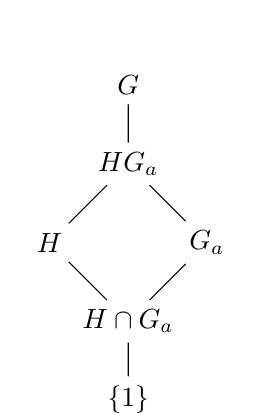
\begin{tikzpicture}
				\node (G) at (0, 0) {$G$};
				\node (HGa) at (0, -1) {$HG_a$};
				\node (H) at (-1, -2) {$H$};
				\node (Ga) at (1, -2) {$G_a$};
				\node (HcapGa) at (0, -3) {$H \cap G_a$};
				\node (1) at (0, -4) {$\{1\}$};

				\draw (1) -- (HcapGa) -- (H) -- (HGa) -- (G);
				\draw (HcapGa) -- (Ga) -- (HGa);
			\end{tikzpicture}
		\end{center}
	\end{solalph}
	\item Let $H$ and $K$ be subgroups of the group $G$. For each $x \in G$ define the $HK$ \textit{double coset} of $x$ in $G$ to be the set $HxK = \{hxk \mid h \in H, k \in K\}$.
	\begin{problems}
		\item Prove that $HxK$ is the union of the left cosets $x_1K, \ldots, x_nK$ where $\{x_1K, \ldots, x_nK\}$ is the orbit containing $xK$ of $H$ acting by left multiplication on the set of left cosets of $K$.
		\item Prove that $HxK$ is a union of right cosets of $H$.
		\item Show that $HxK$ and $HyK$ are either the same set or are disjoint for all $x, y \in G$. Show that the set of $HK$ double cosets partitions $G$.
		\item Prove that $|HxK| = |K| \cdot |H : H \cap xKx^{-1}|$.
		\item Prove that $|HxK| = |H| \cdot |K : K \cap x^{-1}Hx|$.
	\end{problems}
	\begin{solalph}
		\item Let $\oo$ be the orbit containing $xK$ of $H$ acting by left multiplication on the set of left cosets of $K$. Then $\oo = \set{hxK \mid h \in H}$, and let $\{x_1K, \ldots, x_nK\}$ be the distinct left cosets in $\oo$. Let $\kk$ be the union of these left cosets, i.e., $\kk = \bigcup_1^n x_iK$.
		
		Now pick $y \in HxK$. Then there exist $h \in H$ and $k \in K$ such that $y = hxk$. Note that $hxK \in \oo$, so there exists some $i$ such that $hxK = x_iK$. Therefore, $y = hxk \in x_iK \subseteq \kk$, hence $HxK \subseteq \kk$. If $z \in \kk$, then there exists some $i$ and some $k' \in K$ such that $z = x_ik'$. Since $x_iK \in \oo$, then there exists some $h' \in H$ such that $x_iK = h'xK$, hence $x_i = h'xk''$ for some $k'' \in K$. Therefore, $z = x_ik' = h'xkk'' \in HxK$, so $\kk \subseteq HxK$. We have shown that $HxK = \kk$, i.e., $HxK$ is the union of the left cosets $x_1K, \ldots, x_nK$.
		\item The proof is similar to that of part (a). 
		\item Let $x, y \in G$. Suppose $HxK \cap HyK \neq \varnothing$. Then there exist $h_1, h_2 \in H$ and $k_1, k_2 \in K$ such that $h_1 x k_1 = h_2 y k_2$. Rearranging, we have $y = h_2\inv h_1 x k_1 k_2\inv$, hence $y \in HxK$. Therefore, $HyK \subseteq HxK$. By symmetry, we also have $HxK \subseteq HyK$, so $HxK = HyK$. We have shown that $HxK$ and $HyK$ are either the same set or are disjoint for all $x, y \in G$. Since every element of $G$ is in some double coset of the form $HxK$, then the set of $HK$ double cosets partitions $G$.
		\item Recall that the orbit of $xK$ under this action is $\oo = \set{hxK \mid h \in H}$. By Proposition 4.2, we have $|\oo| = |H : H_{xK}|$, where $H_{xK}$ is the stabilizer of $xK$ in $H$. Observe that $H_{xK} = \set{h \in H \mid hxK = xK}$. Then $hxK = xK$ implies that there exists some $k \in K$ such that $hxk = x$, or equivalently, $h = x k x\inv$. Therefore, $H_{xK} = H \cap x K x\inv$. By part (a), we have $|HxK| = |\oo| \cdot |K| = |H : H \cap x K x\inv| \cdot |K|$.
		\item Similar to part (d).
	\end{solalph}
\end{problems}

\newpage

\subsection{Groups Acting on Themselves by Left Mutliplication---Cayley's Theorem}

\begin{problems}
	\item \label{ex4.2.1} Let $G$ be $\{1,a,b,c\}$, the Klein 4-group whose group table is written out in Section 2.5.
	\begin{problems}
		\item Label $1,a,b,c$ with the integers $1,2,4,3$, respectively, and prove that under the left regular representation of $G$ into $S_4$ the nonidentity elements are mapped as follows:
		\[a \mapsto (1\ 2)(3\ 4), \quad b \mapsto (1\ 4)(2\ 3), \quad c \mapsto (1\ 3)(2\ 4).\]
		\item Relabel $1,a,b,c$ as $1,4,2,3$, respectively, and compute the image of each element of $G$ under the left regular representation of $G$ into $S_4$. Show that the image of $G$ in $S_4$ under this labelling is the same \emph{subgroup} as the image of $G$ in part (a) (even though the nonidentity elements individually map to different permutations under the two different labellings).
	\end{problems}
	\begin{solalph}
		\item We have $a \cdot 1 = a$ so that $\sigma_a(1) = 2$. Similarly, $\sigma_a(2) = 1$. We also have $a \cdot b = c$ so that $\sigma_a(4) = 3$, and $\sigma_a(3) = 4$, and we have $a \mapsto (1\ 2)(3\ 4)$. The others are computed similarly. 
		\item Again, we have $a \cdot 1 = a$ so that $\sigma_a(1) = 4$. Similarly, $\sigma_a(4) = 1$. We also have $a \cdot b = c$ so that $\sigma_a(2) = 3$, and $\sigma_a(3) = 2$, and we have $a \mapsto (1\ 4)(2\ 3)$. For $b$, we have $b \mapsto (1\ 2)(3\ 4)$, and for $c$, we have $c \mapsto (1\ 3)(2\ 4)$. The image of $G$ in $S_4$ under this labelling is $\{1, (1\ 4)(2\ 3), (1\ 2)(3\ 4), (1\ 3)(2\ 4)\}$, which is the same subgroup as in part (a).
	\end{solalph}
	\item List the elements of $S_3$ as $1, (1\ 2), (2\ 3), (1\ 3), (1\ 2\ 3), (1\ 3\ 2)$ and label these with the integers $1,2,3,4,5,6$ respectively. Exhibit the image of each element of $S_3$ under the left regular representation of $S_3$ into $S_6$.
	\begin{sol}
		Consider $(1\ 2)$. Then we have the following computations:
		\begin{align*}
			(1\ 2) \cdot 1 & = (1\ 2) && \sigma_{(1\ 2)}(1) = 2 \\
			(1\ 2) \cdot (1\ 2) & = 1 && \sigma_{(1\ 2)}(2) = 1 \\
			(1\ 2) \cdot (2\ 3) & = (1\ 3\ 2) && \sigma_{(1\ 2)}(4) = 5 \\
			(1\ 2) \cdot (1\ 3) & = (1\ 2\ 3) && \sigma_{(1\ 2)}(3) = 6 \\
			(1\ 2) \cdot (1\ 2\ 3) & = (2\ 3) && \sigma_{(1\ 2)}(5) = 3 \\
			(1\ 2) \cdot (1\ 3\ 2) & = (1\ 3) && \sigma_{(1\ 2)}(6) = 4
		\end{align*}
		Thus, we have $(1\ 2) \mapsto (1\ 2)(3\ 6\ 4\ 5)$. We calculate that $(2\ 3) \mapsto (1\ 3\ 5\ 2)(4\ 6)$. Since $(1\ 2)(2\ 3) = (1\ 2\ 3)$, then
		\[(1\ 2\ 3) \mapsto (1\ 2)(3\ 6\ 4\ 5)(1\ 3\ 5\ 2)(4\ 6) = (1\ 5\ 6)(2\ 4\ 3)\]
		Continuing in this way, we find that the images of the elements of $S_3$ under the left regular representation are as follows:
		\begin{align*}
			1 & \mapsto 1 \\
			(1\ 2) & \mapsto (1\ 2)(3\ 6\ 4\ 5) \\
			(2\ 3) & \mapsto (1\ 3\ 5\ 2)(4\ 6) \\
			(1\ 3) & \mapsto (1\ 4)(2\ 6)(3\ 5) \\
			(1\ 2\ 3) & \mapsto (1\ 5\ 6)(2\ 4\ 3) \\
			(1\ 3\ 2) & \mapsto (1\ 6\ 5)(2\ 3\ 4) \qh
		\end{align*}
	\end{sol}
	\item \label{ex4.2.3} Let $r$ and $s$ be the usual generators for the dihedral group of order 8.
	\begin{problems}
		\item List the elements of $D_8$ as $1, r, r^2, r^3, s, sr, sr^2, sr^3$ and label these with the integers $1,2,\dots,8$ respectively. Exhibit the image of each element of $D_8$ under the left regular representation of $D_8$ into $S_8$.
		\item Relabel this same list of elements of $D_8$ with the integers $1,3,5,7,2,4,6,8$ respectively and recompute the image of each element of $D_8$ under the left regular representation with respect to this new labelling. Show that the two subgroups of $S_8$ obtained in parts (a) and (b) are different.
	\end{problems}
	\begin{solalph}
		\item We calculate $\sigma_r = (1\ 2\ 3\ 4)(5\ 8\ 7\ 6)$ and $\sigma_s = (1\ 5)(2\ 6)(3\ 7)(4\ 8)$. Continuing in this way, we find that the images of the elements of $D_8$ under the left regular representation are as follows:
		\begin{align*}
			1 & \mapsto 1 & s & \mapsto (1\ 5)(2\ 6)(3\ 7)(4\ 8) \\
			r & \mapsto (1\ 2\ 3\ 4)(5\ 8\ 7\ 6) & sr & \mapsto (1\ 6)(2\ 7)(3\ 8)(4\ 5) \\
			r^2 & \mapsto (1\ 3)(2\ 4)(5\ 7)(6\ 8) & sr^2 & \mapsto (1\ 7)(2\ 8)(3\ 5)(4\ 6) \\
			r^3 & \mapsto (1\ 4\ 3\ 2)(5\ 6\ 7\ 8) & sr^3 & \mapsto (1\ 8)(2\ 5)(3\ 6)(4\ 7)
		\end{align*}
		\item The images of $D_8$ under the left regular representation with respect to this new labelling are as follows:
		\begin{align*}
			1 & \mapsto 1 & s & \mapsto (1\ 2)(3\ 4)(5\ 6)(7\ 8) \\
			r & \mapsto (1\ 3\ 5\ 7)(2\ 8\ 6\ 4) & sr & \mapsto (1\ 4)(2\ 7)(3\ 6)(5\ 8) \\
			r^2 & \mapsto (1\ 5)(3\ 7)(2\ 6)(4\ 8) & sr^2 & \mapsto (1\ 6)(2\ 5)(3\ 8)(4\ 7) \\
			r^3 & \mapsto (1\ 7\ 5\ 3)(2\ 4\ 6\ 8) & sr^3 & \mapsto (1\ 8)(2\ 3)(4\ 5)(6\ 7)
		\end{align*}
		Clearly, the two subgroups of $S_8$ obtained in parts (a) and (b) are different since, for example, the image of $r$ in part (a) is a product of two 4-cycles while the image of $r$ in part (b) is a product of two 4-cycles but with different elements.
	\end{solalph}
	\item \label{ex4.2.4} Use the left regular representation of $Q_8$ to produce two elements of $S_8$ which generate a subgroup of $S_8$ isomorphic to the quaternion group $Q_8$.
	\begin{sol}
		At minimum, we have that $Q_8 = \gen{i, j}$ (any 2 elements of order 4 can be used), so we compute the images of $i$ and $j$ under the left regular representation. We label $Q_8$ as $1, -1, i, -i, j, -j, k, -k$ and label these with the integers $1,2 \ldots 8$ respectively. We find that
		\begin{align*}
			i & \mapsto \sigma_i = (1\ 3\ 4\ 2)(5\ 7)(6\ 8) \\
			j & \mapsto \sigma_j = (1\ 5\ 2\ 6)(3\ 8)(4\ 7)
		\end{align*}
		Hence $Q_8 \cong \gen{\sigma_i, \sigma_j} \leq S_8$.
	\end{sol}
	\item \label{ex4.2.5} Let $r$ and $s$ be the usual generators for the dihedral group of order 8 and let $H = \langle s \rangle$. List the left cosets of $H$ in $D_8$ as $1H, rH, r^2H$ and $r^3H$.
	\begin{problems}
		\item Label these cosets with the integers $1,2,3,4$, respectively. Exhibit the image of each element of $D_8$ under the representation $\pi_H$ of $D_8$ into $S_4$ obtained from the action of $D_8$ by left multiplication on the set of 4 left cosets of $H$ in $D_8$. Deduce that this representation is faithful (i.e., the elements of $S_4$ obtained form a subgroup isomorphic to $D_8$).
		\item Repeat part (a) with the list of cosets relabelled by the integers $1,3,2,4$, respectively. Show that the permutations obtained from this labelling form a subgroup of $S_4$ that is different from the subgroup obtained in part (a).
		\item Let $K = \langle sr \rangle$, list the cosets of $K$ in $D_8$ as $1K, rK, r^2K$ and $r^3K$, and label these with the integers $1,2,3,4$. Prove that, with respect to this labelling, the image of $D_8$ under the representation $\pi_K$ obtained from left multiplication on the cosets of $K$ is the same \emph{subgroup} of $S_4$ as in part (a) (even though the subgroups $H$ and $K$ are different and some of the elements of $D_8$ map to different permutations under the two homomorphisms).
	\end{problems}
	\begin{solalph}
		\item We have $\pi_H(r) = (1\ 2\ 3\ 4)$ and $\pi_H(s) = (2\ 4)$. We continue in this way to find that the images of the elements of $D_8$ under $\pi_H$ are:
		\begin{align*}
			\pi_H(1) & = 1 & \pi_H(s) & = (2\ 4) \\
			\pi_H(r) & = (1\ 2\ 3\ 4) & \pi_H(sr) & = (1\ 2)(3\ 4) \\
			\pi_H(r^2) & = (1\ 3)(2\ 4) & \pi_H(sr^2) & = (1\ 3) \\
			\pi_H(r^3) & = (1\ 4\ 3\ 2) & \pi_H(sr^3) & = (1\ 4)(2\ 3)
		\end{align*}
		so that the subgroup $\gen{\pi_H(r), \pi_H(s)} \leq S_4$ is isomorphic to $D_8$. Since the kernel of $\pi_H$ is trivial, then the representation is faithful.
		\item The new labelling affords the permutations $\pi_H(r) = (1\ 3\ 2\ 4)$ and $\pi_H(s) = (3\ 4)$. We have the following images:
		\begin{align*}
			\pi_H(1) & = 1 & \pi_H(s) & = (3\ 4) \\
			\pi_H(r) & = (1\ 3\ 2\ 4) & \pi_H(sr) & = (1\ 3)(2\ 4) \\
			\pi_H(r^2) & = (1\ 2)(3\ 4) & \pi_H(sr^2) & = (1\ 2) \\
			\pi_H(r^3) & = (1\ 4\ 2\ 3) & \pi_H(sr^3) & = (1\ 4)(2\ 3)
		\end{align*}
		Moreover, the subgroup is different from that in part (a) since, for example, the image of $r$ in part (a) is $(1\ 2\ 3\ 4)$ while the image of $r$ in this part is $(1\ 3\ 2\ 4)$.
		\item Under $\pi_K$, we have $\pi_K(r) = (1\ 2\ 3\ 4)$ and $\pi_K(s) = (1\ 2)(3\ 4)$. With respect to this labeling, we have the subgroup $\wh K = \gen{(1\ 2\ 3\ 4), (1\ 2)(3\ 4)}$. Let $\wh H$ be the subgroup obtained in part (a). Note that $(1\ 2\ 3\ 4)$ is contained in both $\wh H$ and $\wh K$. Moreover, we have following:
		\[(1\ 2\ 3\ 4)(2\ 4)(1\ 4\ 3\ 2) = (1\ 2)(3\ 4) \in \wh H \longand (1\ 2\ 3\ 4)^2(1\ 2)(3\ 4) = (2\ 4) \in \wh K\]
		so that both subgroups contain the other generator of the other subgroup. Therefore, $\wh H = \wh K$.
	\end{solalph}
    \item Let $r$ and $s$ be the usual generators for the dihedral group of order 8 and let $N = \langle r^2 \rangle$. List the left cosets of $N$ in $D_8$ as $1N, rN, sN$ and $srN$. Label these cosets with the integers $1,2,3,4$ respectively. Exhibit the image of each element of $D_8$ under the representation $\pi_N$ of $D_8$ into $S_4$ obtained from the action of $D_8$ by left multiplication on the set of 4 left cosets of $N$ in $D_8$. Deduce that this representation is not faithful and prove that $\pi_N(D_8)$ is isomorphic to the Klein 4-group.
	\begin{sol}
		We have $\pi_N(r) = (1\ 2)(3\ 4)$ and $\pi_N(s) = (1\ 3)(2\ 4)$. Continuing in this way, we find that the images of the elements of $D_8$ under $\pi_N$ are:
		\begin{align*}
			\pi_N(1) & = 1 & \pi_N(s) & = (1\ 3)(2\ 4) \\
			\pi_N(r) & = (1\ 2)(3\ 4) & \pi_N(sr) & = (1\ 4)(2\ 3) \\
			\pi_N(r^2) & = 1 & \pi_N(sr^2) & = (1\ 3)(2\ 4) \\
			\pi_N(r^3) & = (1\ 2)(3\ 4) & \pi_N(sr^3) & = (1\ 4)(2\ 3)
		\end{align*}
		Since $\ker(\pi_N)$ contains the nontrivial element $r^2$, then the representation is not faithful. Moreover, we have $\pi_N(D_8) = \{1, (1\ 2)(3\ 4), (1\ 3)(2\ 4), (1\ 4)(2\ 3)\}$, which is isomorphic to the Klein 4-group.
	\end{sol}
    \item Let $Q_8$ be the quaternion group of order 8.
	\begin{problems}
		\item Prove that $Q_8$ is isomorphic to a subgroup of $S_8$.
		\item Prove that $Q_8$ is not isomorphic to a subgroup of $S_n$ for any $n \le 7$. [If $Q_8$ acts on any set $A$ of order $\le 7$ show that the stabilizer of any point $a \in A$ must contain the subgroup $\langle -1 \rangle$.]
	\end{problems}
	\begin{solalph}
		\item This is done in \hyperref[ex4.2.4]{Exercise 4.2.4}.
		\item Let $Q_8$ act on a set $A$ of order $n \leq 7$. For any $a \in A$, consider the orbit $\oo_a$ of $a$ under this action. By Proposition 4.2, we have $|\oo_a| = |Q_8 : (Q_8)_a|$, where $(Q_8)_a$ is the stabilizer of $a$ in $Q_8$. Since $|\oo_a|$ divides $|A| \leq 7$, then $|\oo_a|$ must be 1, 2, 4, or 7. However, since $Q_8$ has no subgroup of index 7, then $|\oo_a|$ cannot be 7. If $|\oo_a| = 4$, then $(Q_8)_a$ has order 2, but the only subgroup of order 2 in $Q_8$ is $\langle -1 \rangle$. If $|\oo_a| = 2$, then $(Q_8)_a$ has order 4, and the only subgroups of order 4 in $Q_8$ are $\langle i \rangle$, $\langle j \rangle$, and $\langle k \rangle$, all of which contain $\langle -1 \rangle$. If $|\oo_a| = 1$, then $(Q_8)_a = Q_8$, which also contains $\langle -1 \rangle$. Therefore, in all cases, the stabilizer $(Q_8)_a$ contains $\langle -1 \rangle$. Since this holds for all $a \in A$, then $\langle -1 \rangle$ is contained in the kernel of the action. The action is not faithful, hence $Q_8$ cannot be isomorphic to a subgroup of $S_n$ for any $n \leq 7$.
	\end{solalph}
    \item Prove that if $H$ has finite index $n$ then there is a normal subgroup $K$ of $G$ with $K \le H$ and $|G : K| \le n!$.
	\begin{sol}
		Let $G$ act by left multiplication on the set of left cosets of $H$ in $G$. Then we have the homomorphism $\phi : G \to S_n$, which is the permutation representation of $G$ on $G/H$. Let $K = \ker(\phi) \subseteq H$, since $g \in K$ if and only if $gH = H$. By the First Isomorphism Theorem, we have $G/K \cong \phi(G) \leq S_n$, so that $|G : K| = |G/K| = |\phi(G)|$ divides $n!$. Therefore, $|G : K| \leq n!$.
	\end{sol}
    \item Prove that if $p$ is a prime and $G$ is a group of order $p^\alpha$ for some $\alpha \in \mathbb{Z}^+$, then every subgroup of index $p$ is normal in $G$. Deduce that every group of order $p^2$ has a normal subgroup of order $p$.
	\begin{sol}
		Let $H$ be a subgroup of $G$ with index $p$. Then $|G : H| = p$, so the action of $G$ on the left cosets of $H$ in $G$ gives a homomorphism $\phi : G \to S_p$. Since $|G| = p^\alpha$, then by Lagrange's Theorem, the order of $\phi(G)$ divides $p^\alpha$. However, the only subgroups of $S_p$ whose order divides $p^\alpha$ are the trivial group and groups of order $p$. Since $\phi(G)$ acts transitively on the $p$ cosets of $H$, then $\phi(G)$ cannot be trivial. Therefore, $|\phi(G)| = p$, which is prime, so $\phi(G)$ is cyclic and hence abelian. The kernel of $\phi$ is a normal subgroup of $G$ contained in $H$. Since the image $\phi(G)$ has order $p$, then by the First Isomorphism Theorem, we have $|G : \ker(\phi)| = p$. But since $\ker(\phi) \subseteq H$ and both have index $p$, then $\ker(\phi) = H$. Therefore, $H$ is normal in $G$.

		To deduce that every group of order $p^2$ has a normal subgroup of order $p$, let $G$ be a group of order $p^2$. By Cauchy's Theorem, there exists an element of order $p$ in $G$, which generates a subgroup $H$ of order $p$. Since the index of $H$ in $G$ is $p$, by the previous result, $H$ is normal in $G$.
	\end{sol}
    \item Prove that every non-abelian group of order 6 has a nonnormal subgroup of order 2. Use this to classify groups of order 6. [Produce an injective homomorphism into $S_3$.]
	\begin{sol}
		Note that $2 \mid 6$ and $3 \mid 6$. By Cauchy's Theorem, there exists subgroups $H$ and $K$ of orders 2 and 3 respectively. Let $H = \set{1, h}$, suppose it is normal, and let $g \in G - H$. Since $H \nsub G$, then $gHg\inv = H$. In particular, $ghg\inv \in H$, so either $ghg\inv = 1$ or $ghg\inv = h$. Since the first case implies $h = 1$, it must be that $ghg\inv = h$, or $gh = hg$. Then $h$ commutes with every element. Moreover, we may use \hyperref[ex3.3.3]{Exercise 3.3.3} to conclude that $G = HK$ since $H \nsub G$. Since $K$ is also abelian as it is cyclic, then $G = hk$ for $h \in H$ and $k \in K$, implying that $G$ is abelian, a contradiction. Therefore, $H$ is not normal in $G$.

		To classify groups of order 6, let $G$ be a group of order 6. If $G$ is abelian, then $G \cong \z_6 \cong \z_2 \times \z_3$. If $G$ is non-abelian, then by the above result, $G$ has a nonnormal subgroup $H$ of order 2. Let $K$ be the subgroup of order 3. Then $G = HK$. Let $G$ act by left multiplication on the left cosets of $K$ in $G$. This action gives a homomorphism $\phi : G \to S_3$. Since $H$ is not normal in $G$, then the action is nontrivial, so $\phi$ is injective. Therefore, $G \cong \phi(G) \leq S_3$. Since $|G| = 6 = |S_3|$, then $\phi(G) = S_3$, and hence $G \cong S_3$.
	\end{sol}
    \item \label{ex4.2.11} Let $G$ be a finite group and let $\pi : G \to S_G$ be the left regular representation. Prove that if $x$ is an element of $G$ of order $n$ and $|G| = mn$, then $\pi(x)$ is a product of $m$ $n$-cycles. Deduce that $\pi(x)$ is an odd permutation if and only if $|x|$ is even and $\abs G/\abs x$ is odd.
	\begin{sol}
		Let $x \in G$ with $\abs x = n$. Consider the action of $\langle x \rangle$ on $G$ by left multiplication. The orbit of any $g \in G$ under this action is $\oo_g = \set{x^k g \mid k = 0, 1, \ldots, n-1}$. Since $\abs x = n$, then $|\oo_g| = n$ for all $g \in G$. By Proposition 4.2, we have $|\oo_g| = |\langle x \rangle : (\langle x \rangle)_g|$, where $(\langle x \rangle)_g$ is the stabilizer of $g$ in $\langle x \rangle$. Since $|\oo_g| = n$, then $(\langle x \rangle)_g$ is trivial for all $g \in G$. Therefore, the orbits of this action partition $G$ into subsets of size $n$. Since $|G| = mn$, there are exactly $m$ such orbits. Each orbit corresponds to an $n$-cycle in the permutation $\pi(x)$. Therefore, $\pi(x)$ is a product of $m$ $n$-cycles.

		To determine when $\pi(x)$ is an odd permutation, we note that an $n$-cycle is an odd permutation if and only if $n$ is even. Since $\pi(x)$ is a product of $m$ $n$-cycles, the parity of $\pi(x)$ is determined by the parity of $m$ and $n$. Specifically, $\pi(x)$ is odd if and only if $n$ is even and $m$ is odd. Thus, $\pi(x)$ is an odd permutation if and only if $|x|$ is even and $|G|/|x|$ is odd.
	\end{sol}
    \item \label{ex4.2.12} Let $G$ and $\pi$ be as in the preceding exercise. Prove that if $\pi(G)$ contains an odd permutation then $G$ has a subgroup of index 2. [Use \hyperref[ex3.3.3]{Exercise 3.3.3}.]
	\begin{sol}
		Recall the $\ep$ homomorphism from Proposition 3.23. Moreover, $\pi$ is a homomorphism from $G$ to $S_G$. Consider the composition $\ep \circ \pi : G \to \set{\pm 1}$. Since $\pi(G)$ contains an odd permutation, then $\ep \circ \pi$ is surjective. By the First Isomorphism Theorem, we have $G/\ker(\ep \circ \pi) \cong \set{\pm 1}$, so that $|\ker(\ep \circ \pi)| = |G|/2$. Therefore, $\ker(\ep \circ \pi)$ is a subgroup of $G$ of index 2.
	\end{sol}
    \item Prove that if $|G| = 2k$ where $k$ is odd then $G$ has a subgroup of index 2. [Use Cauchy's Theorem to produce an element of order 2 and then use the preceding two exercises.]
	\begin{sol}
		By Cauchy's Theorem, there exists $x \in G$ such that $\abs x = 2$. Then $\pi(x)$ is of order 2 and is hence a product of disjoint transpositions. Since $|G| = 2k$ with $k$ odd, then use $m = k$ and $n = 2$ in \hyperref[ex4.2.11]{Exercise 4.2.11} along with even $\abs x$ to conclude that $\pi(x)$ is an odd permutation. By the \hyperref[ex4.2.12]{Exercise 4.2.12}, $G$ has a subgroup of index 2.
	\end{sol}
    \item Let $G$ be a finite group of composite order $n$ with the property that $G$ has a subgroup of order $k$ for each positive integer $k$ dividing $n$. Prove that $G$ is not simple.
    \begin{sol}
		Let $S$ be the set of all prime factors of $n$. By the Well Ordering Principle, this has a minimal element $p$. By hypothesis, $G$ has a subgroup $P$ of order $n/p$ with index $p$. By Corollary 4.5, $P$ is normal in $G$ since $p$ is the smallest prime dividing $n$. Therefore, $G$ is not simple.
	\end{sol}
\end{problems}

\newpage

\subsection{Groups Acting on Themselves by Conjugation---The Class Equation}

Let $G$ be a group.

\begin{problems}
	\item  Suppose $G$ has a left action on a set $A$, denoted by $g \cdot a$ for all $g \in G$ and $a \in A$. Denote the corresponding right action on $A$ by $a \cdot g$. Prove that the (equivalence) relations $\sim$ and $\sim'$ defined by
	\[ a \sim b \quad \text{if and only if} \quad a = g \cdot b \quad \text{ for some } g \in G \]
	and
	\[ a \sim' b \quad \text{if and only if} \quad a = b \cdot g \quad \text{ for some } g \in G \]
	are the same relation (i.e., $a \sim b$ if and only if $a \sim' b$).
	\begin{sol}
		If $a \sim b$, there exists $g \in G$ such that $a = g \cdot b$. Let $h = g\inv$. Then $b = h \cdot a$, so $a = b \cdot g$. Thus, $a \sim' b$. Conversely, if $a \sim' b$, there exists $g \in G$ such that $a = b \cdot g$. Let $h = g\inv$. Then $b = h \cdot a$, so $a = g \cdot b$. Thus, $a \sim b$. Therefore, the relations $\sim$ and $\sim'$ are the same.
	\end{sol}
	\item \label{ex4.3.2} Find all conjugacy classes and their sizes in the following groups:
	\begin{problems}
		\item $D_8$
		\item $Q_8$
		\item $A_4$
	\end{problems}
	\begin{solalph}
		\item Discussed in the text, the conjugacy classes of $D_8$ are $\{1\}$, $\{r^2\}$, $\{r, r^3\}$, $\{s, sr^2\}$, and $\{sr, sr^3\}$ with sizes 1, 1, 2, 2, and 2 respectively.
		\item Again discussed in the text, the conjugacy classes of $Q_8$ are $\{1\}$, $\{-1\}$, $\{i, -i\}$, $\{j, -j\}$, and $\{k, -k\}$ with sizes 1, 1, 2, 2, and 2 respectively.
		\item We proceed similarly as the text. The possible cycle types are $1, (1\ 2\ 3)$, and $(1\ 2)(3\ 4)$.
		
		For $(1\ 2\ 3)$, we have $C_{A_4}((1\ 2\ 3)) = \gen{(1\ 2\ 3)}$ since the only permutation that fixes 1, 2, and 3 is the identity. Therefore, the conjugacy class of $(1\ 2\ 3)$ has size $12/3 = 4$. However, there are 8 3-cycles in $A_4$, so there exists a 3-cycle $\sigma \in A_4$ not in the conjugacy class of $(1\ 2\ 3)$. By similar reasoning, the conjugacy class of $\sigma$ also has size 4. There are then 2 conjugacy classes of size 4 corresponding to the 3-cycles.

		For $(1\ 2)(3\ 4)$, it is trivial to calculate that the remaining double transpositions are in its conjugacy class. Therefore, the conjugacy class of $(1\ 2)(3\ 4)$ has size 3.
	\end{solalph}
	\item Find all conjugacy classes and their sizes in the following groups:
	\begin{problems}
		\item $Z_2 \times S_3$
		\item $S_3 \times S_3$
		\item $Z_3 \times A_4$
	\end{problems}
	\begin{sol}
		We first prove a (somewhat) trivial idea: if $G$ and $H$ are groups, let $g \in G$ and $h \in H$. Let $\kk_g$ and $\kk_h$ be the conjugacy classes of $g$ in $G$ and $h$ in $H$ respectively. Then $\kk_{(g,h)} = \kk_g \times \kk_h$ is the conjugacy class of $(g,h)$ in $G \times H$. To see this, note that for any $(x,y) \in G \times H$, we have
		\[(x,y)(g,h)(x,y)\inv = (xgx\inv, yhy\inv) \in \kk_g \times \kk_h.\]
		Conversely, for any $(g', h') \in \kk_g \times \kk_h$, there exist $x \in G$ and $y \in H$ such that $g' = xgx\inv$ and $h' = yhy\inv$. Therefore, $(g', h') = (x,y)(g,h)(x,y)\inv$, so $(g', h')$ is in the conjugacy class of $(g,h)$ in $G \times H$. This result shows two important things: the conjugacy classes of $G \times H$ are precisely the products of the conjugacy classes of $G$ and $H$, and the size of the conjugacy class of $(g,h)$ in $G \times H$ is the product of the sizes of the conjugacy classes of $g$ in $G$ and $h$ in $H$. We now use this to answer the question.
		\begin{problems}
			\item Let $Z_2 = \gen x$. The conjugacy classes $\kk_1$ and $\kk_x$ of $Z_2$ have sizes 1 and 1 respectively. For $S_3$, the partitions of 3 are 3 1-cycles, 2-cycle and 1-cycle, and a 3-cycle with representatives $1$, $(1\ 2)$, and $(1\ 2\ 3)$ respectively. Since $C_{S_3}((1\ 2)) = \gen{(1\ 2)}$ and $C_{S_3}((1\ 2\ 3)) = \gen{(1\ 2\ 3)}$, then the conjugacy classes $\kk_1$, $\kk_{(1\ 2)}$, and $\kk_{(1\ 2\ 3)}$ of $S_3$ have sizes 1, 3, and 2 respectively. Therefore, $Z_2 \times S_3$ has 6 conjugacy classes of size 1, 3, 2, 1, 3, and 2 respectively.
			\item By the above, $S_3$ has 3 conjugacy classes of sizes 1, 3, and 2 respectively. Then $S_3 \times S_3$ has 9 conjugacy classes with sizes $1, 3, 2, 3, 9, 6, 2, 6,$ and $4$ respectively.
			\item $Z_3$ has 3 conjugacy classes of size 1 each. From \hyperref[ex4.3.2]{Exercise 4.3.2}, we know that $A_4$ has 4 conjugacy classes of sizes 1, 4, 4, and 3. Therefore, $Z_3 \times A_4$ has 12 conjugacy classes with sizes $1, 4, 4, 3, 1, 4, 4, 3, 1, 4, 4,$ and $3$ respectively. \qh
		\end{problems}
	\end{sol}
	\item Prove that if $S \subseteq G$ and $g \in G$ then $gN_G(S)g^{-1} = N_G(gSg^{-1})$ and $gC_G(S)g^{-1} = C_G(gSg^{-1}).$
	\begin{sol}
		Suppose $x \in gN_G(S)g\inv$, and consider $xgSg\inv x\inv$. Since $x = gng\inv$ for some $n \in N_G(S)$, then we have $gng\inv gSg\inv gn\inv g\inv = g n S n\inv g\inv = g S g\inv$, so that $x \in N_G(gSg\inv)$. Conversely, suppose $x \in N_G(gSg\inv)$. Then $xgSg\inv x\inv = gSg\inv$. Letting $n = g\inv x g$, we have $n S n\inv = S$, so $n \in N_G(S)$ and hence $x \in gN_G(S)g\inv$. Therefore, $gN_G(S)g\inv = N_G(gSg\inv)$.

		Suppose $x \in gC_G(S)g\inv$, and consider $xsx\inv$ for some $s \in gSg\inv$. Since $x = gng\inv$ for some $n \in C_G(S)$, then we have $gng\inv s g n\inv g\inv = g n (g\inv s g) n\inv g\inv = g (g\inv s g) g\inv = s$, so that $x \in C_G(gSg\inv)$. Conversely, suppose $x \in C_G(gSg\inv)$. Then $xsx\inv = s$ for all $s \in gSg\inv$. Letting $n = g\inv x g$, we have $n t n\inv = t$ for all $t \in S$, so $n \in C_G(S)$ and hence $x \in gC_G(S)g\inv$. Therefore, $gC_G(S)g\inv = C_G(gSg\inv)$.
	\end{sol}
	\item If the center of $G$ is of index $n$, prove that every conjugacy class has at most $n$ elements.
	\begin{sol}
		Let $\kk_g$ be the conjugacy class of some $g \in G$. By Proposition 4.6, we have $|\kk_g| = |G : C_G(g)|$. Since $Z(G) \leq C_G(g)$ for all $g \in G$, Lagrange's Theorem shows that $|Z(G)|$ divides $|C_G(g)|$. Therefore, $|G : C_G(g)|$ divides $|G : Z(G)| = n$. Hence, $|\kk_g| \leq n$.
	\end{sol}
	\item Assume $G$ is a non-abelian group of order $15$. Prove that $Z(G)=1$. Use the fact that $\langle g \rangle \le C_G(g)$ for all $g \in G$ to show that there is at most one possible class equation for $G$. [Use \hyperref[ex3.1.36]{Exercise 3.1.36}.]
	\begin{sol}
		Recall that $Z(G) \leq G$. Since $G$ is non-abelian, then $Z(G) \neq G$. Assume $1 < Z(G) < 15$. By Lagrange's Theorem, $Z(G)$ has order 3 or 5. If $|Z(G)| = 3$, then $|G/Z(G)| = 5$ and $G/Z(G) \cong Z_5$. If $|Z(G)| = 5$, then $|G/Z(G)| = 3$ and $G/Z(G) \cong Z_3$. In either case, $G/Z(G)$ is cyclic by Corollary 3.10, and \hyperref[ex3.1.36]{Exercise 3.1.36} implies that $G$ is abelian, a contradiction. Therefore, $Z(G) = 1$.

		Now suppose $g \in G$ is nonidentity. Since $\langle g \rangle \leq C_G(g)$, then $|C_G(g)|$ is 3, 5, or 15 by Lagrange's Theorem. If $|C_G(g)| = 15$, then $C_G(g) = G$, so $g \in Z(G)$, a contradiction. Therefore, $|C_G(g)|$ is 3 or 5 for all nonidentity $g \in G$. By Proposition 4.6, we have $|\kk_g| = |G : C_G(g)|$, so that $|\kk_g|$ is 5 or 3 respectively. The identity element forms a conjugacy class of size 1, and the class equation must involve a summation of sizes 3 and 5 that adds to 14. The only such combination is three classes of size 3 and one class of size 5. Therefore, the class equation of $G$ is $15 = 1 + 3 + 3 + 3 + 5$.
	\end{sol}
	\item For $n=3,4,6,$ and $7$ make lists of the partitions of $n$ and give representatives for the corresponding conjugacy classes of $S_n$.
	\begin{sol}
		$n = 3$:
		\[\begin{array}{c|c}
			\textbf{Partition of 3} & \textbf{Representative of Cycle Type} \\
			\hline
			1, 1, 1 & 1 \\
			2, 1 & (1\ 2) \\
			3 & (1\ 2\ 3)
		\end{array}\]
		$n = 4$:
		\[\begin{array}{c|c}
			\textbf{Partition of 4} & \textbf{Representative of Cycle Type} \\
			\hline
			1, 1, 1, 1 & 1 \\
			2, 1, 1 & (1\ 2) \\
			2, 2 & (1\ 2)(3\ 4) \\
			3, 1 & (1\ 2\ 3) \\
			4 & (1\ 2\ 3\ 4)
		\end{array}\]
		$n = 6$:
		\[\begin{array}{c|c}
			\textbf{Partition of 6} & \textbf{Representative of Cycle Type} \\
			\hline
			1, 1, 1, 1, 1, 1 & 1 \\
			2, 1, 1, 1, 1 & (1\ 2) \\
			2, 2, 1, 1 & (1\ 2)(3\ 4) \\
			2, 2, 2 & (1\ 2)(3\ 4)(5\ 6) \\
			3, 1, 1, 1 & (1\ 2\ 3) \\
			3, 2, 1 & (1\ 2\ 3)(4\ 5) \\
			3, 3 & (1\ 2\ 3)(4\ 5\ 6) \\
			4, 1, 1 & (1\ 2\ 3\ 4) \\
			4, 2 & (1\ 2\ 3\ 4)(5\ 6) \\
			5, 1 & (1\ 2\ 3\ 4\ 5) \\
			6 & (1\ 2\ 3\ 4\ 5\ 6)
		\end{array}\]
		$n = 7$:
		\[\begin{array}{c|c}
			\textbf{Partition of 7} & \textbf{Representative of Cycle Type} \\
			\hline
			1, 1, 1, 1, 1, 1, 1 & 1 \\
			2, 1, 1, 1, 1, 1 & (1\ 2) \\
			2, 2, 1, 1, 1 & (1\ 2)(3\ 4) \\
			2, 2, 2, 1 & (1\ 2)(3\ 4)(5\ 6) \\
			3, 1, 1, 1, 1 & (1\ 2\ 3) \\
			3, 2, 1, 1 & (1\ 2\ 3)(4\ 5) \\
			3, 2, 2 & (1\ 2\ 3)(4\ 5)(6\ 7) \\
			3, 3, 1 & (1\ 2\ 3)(4\ 5\ 6) \\
			4, 1, 1, 1 & (1\ 2\ 3\ 4) \\
			4, 2, 1 & (1\ 2\ 3\ 4)(5\ 6) \\
			4, 3 & (1\ 2\ 3\ 4)(5\ 6\ 7) \\
			5, 1, 1 & (1\ 2\ 3\ 4\ 5) \\
			5, 2 & (1\ 2\ 3\ 4\ 5)(6\ 7) \\
			6, 1 & (1\ 2\ 3\ 4\ 5\ 6) \\
			7 & (1\ 2\ 3\ 4\ 5\ 6\ 7)
		\end{array} \qh\]
	\end{sol}
	\item Prove that $Z(S_n)=1$ for all $n \ge 3$.
	\begin{sol}
		Suppose $\sigma \in Z(S_n)$ for some $n \geq 3$. Then $\sigma$ commutes with every element of $S_n$. In particular, $\sigma$ commutes with all transpositions (the set of which generate $S_n$). Let $(a\ b)$ be any transposition in $S_n$. Then we have $\sigma(a\ b)\sigma\inv = (a\ b)$. This implies that $(\sigma(a)\ \sigma(b)) = (a\ b)$, so $\sigma(a) = a$ and $\sigma(b) = b$. Since $a$ and $b$ were arbitrary, $\sigma$ fixes every element of $\{1, 2, \ldots, n\}$. Therefore, $\sigma$ is the identity permutation. Hence, $Z(S_n) = \{1\}$ for all $n \geq 3$.
	\end{sol}
	\item Show that $|C_{S_n}((1\ 2)(3\ 4))| = 8 (n-4)!$ for all $n \ge 4$. Determine the elements in this centralizer explicitly.
	\begin{sol}
		The $(n - 4)!$ factor arises from the fact that permutations on the $n - 4$ integers not involved in the cycle $(1\ 2)(3\ 4)$ commute with it. Therefore, we need only consider the permutations of $\{1, 2, 3, 4\}$ that commute with $(1\ 2)(3\ 4)$. Computing $C_{S_4}((1\ 2)(3\ 4))$ directly, the permutations that fall in this set need to leave $(1\ 2)(3\ 4)$ unchanged, or swap the two transpositions. The permutations that leave $(1\ 2)(3\ 4)$ unchanged are $1$, $(1\ 2)$, $(3\ 4)$, and $(1\ 2)(3\ 4)$. The permutations that swap the two transpositions are $(1\ 3)(2\ 4)$, $(1\ 4)(2\ 3)$, $(1\ 3\ 2\ 4)$, and $(1\ 4\ 2\ 3)$. Therefore, 
		\[C_{S_4}((1\ 2)(3\ 4)) = \{1, (1\ 2), (3\ 4), (1\ 2)(3\ 4), (1\ 3)(2\ 4), (1\ 4)(2\ 3), (1\ 3\ 2\ 4), (1\ 4\ 2\ 3)\},\]
		which has size 8. Combining this with the $(n - 4)!$ factor, we have $|C_{S_n}((1\ 2)(3\ 4))| = 8(n - 4)!$ for all $n \geq 4$.
	\end{sol}
	\item Let $\sigma$ be the 5-cycle $(1\ 2\ 3\ 4\ 5)$ in $S_5$. In each of (a) to (c) find an explicit element $\tau \in S_5$ which accomplishes the specified conjugation:
	\begin{problems}
		\item $\tau \sigma \tau^{-1} = \sigma^2$
		\item $\tau \sigma \tau^{-1} = \sigma^{-1}$
		\item $\tau \sigma \tau^{-1} = \sigma^{-2}$
	\end{problems}
	\begin{solalph}
		\item $\sigma^2 = (1\ 3\ 5\ 2\ 4)$. Then $\tau = (2\ 3\ 5\ 4)$.
		\item $\sigma^{-1} = (1\ 5\ 4\ 3\ 2)$. Then $\tau = (1\ 5)(2\ 4)$.
		\item $\sigma^{-2} = (1\ 4\ 2\ 5\ 3)$. Then $\tau = (2\ 4\ 5\ 3)$.
	\end{solalph}
	\item In each of (a) -- (d) determine whether $\sigma_1$ and $\sigma_2$ are conjugate. If they are, given an explicit permutation $\tau$ such that $\tau \sigma_1 \tau^{-1} = \sigma_2$.
	\begin{problems}
		\item $\sigma_1 = (1\ 2)(3\ 4\ 5)$ and $\sigma_2 = (1\ 2\ 3)(4\ 5)$
		\item $\sigma_1 = (1\ 5)(3\ 7\ 2)(10\ 6\ 8\ 11)$ and $\sigma_2 = (3\ 7\ 5\ 10)(4\ 9)(13\ 11\ 2)$
		\item $\sigma_1 = (1\ 5)(3\ 7\ 2)(10\ 6\ 8\ 11)$ and $\sigma_2 = \sigma_1^3$
		\item $\sigma_1 = (1\ 3)(2\ 4\ 6)$ and $\sigma_2 = (3\ 5)(2\ 4)(5\ 6)$
	\end{problems}
	\begin{solalph}
		\item Rewrite $\sigma_2$ as $(4\ 5)(1\ 2\ 3)$ so that both have the same cycle type. Then $\tau = (1\ 4\ 2\ 5\ 3)$.
		\item Rewrite $\sigma_2$ as $(4\ 9)(13\ 11\ 2)(3\ 7\ 5\ 10)$. Then $\tau = (1\ 4)(8\ 5\ 9)(6\ 7\ 11\ 10\ 3\ 13)$.
		\item Note that $\sigma_2 = (1\ 5)(6\ 10\ 11\ 8)$, which does not have the same cycle type as $\sigma_1$. Therefore, they are not conjugate.
		\item $\sigma_2 = (2\ 4)(3\ 5\ 6)$. Then $\tau = (1\ 2\ 3\ 4\ 5)$.
	\end{solalph}
	\item Find a representative for each conjugacy class of elements of order $4$ in $S_8$ and $S_{12}$.
	\begin{sol}
		$S_8$:
		\[\begin{array}{c|c}
			\textbf{Cycle Type} & \textbf{Representative} \\
			\hline
			4, 4 & (1\ 2\ 3\ 4)(5\ 6\ 7\ 8) \\
			4, 2, 2 & (1\ 2\ 3\ 4)(5\ 6)(7\ 8) \\
			4, 2, 1, 1 & (1\ 2\ 3\ 4)(5\ 6) \\
			4, 1, 1, 1, 1 & (1\ 2\ 3\ 4)
		\end{array}\]
		$S_{12}$:
		\[\begin{array}{c|c}
			\textbf{Cycle Type} & \textbf{Representative} \\
			\hline
			4, 4, 4 & (1\ 2\ 3\ 4)(5\ 6\ 7\ 8)(9\ 10\ 11\ 12) \\
			4, 4, 2, 2 & (1\ 2\ 3\ 4)(5\ 6\ 7\ 8)(9\ 10)(11\ 12) \\
			4, 4, 2, 1, 1 & (1\ 2\ 3\ 4)(5\ 6\ 7\ 8)(9\ 10) \\
			4, 4, 1, 1, 1, 1 & (1\ 2\ 3\ 4)(5\ 6\ 7\ 8) \\
			4, 2, 2, 2, 2 & (1\ 2\ 3\ 4)(5\ 6)(7\ 8)(9\ 10)(11\ 12) \\
			4, 2, 2, 2, 1, 1 & (1\ 2\ 3\ 4)(5\ 6)(7\ 8)(9\ 10) \\
			4, 2, 2, 1, 1, 1, 1 & (1\ 2\ 3\ 4)(5\ 6)(7\ 8) \\
			4, 2, 1, 1, 1, 1, 1, 1 & (1\ 2\ 3\ 4)(5\ 6) \\
			4, 1, 1, 1, 1, 1, 1, 1, 1 & (1\ 2\ 3\ 4)
		\end{array} \qh\]
	\end{sol}
	\item Find all finite groups which have exactly two conjugacy classes.
	\begin{sol}
		Let $G$ be a finite group with exactly two conjugacy classes. One of these classes must be $\{1\}$, the identity element. Let $\kk$ be the other conjugacy class, and let $g \in \kk$. By Proposition 4.6, we have $|\kk| = |G : C_G(g)|$. Since there are only two conjugacy classes, then $|\kk| = |G| - 1$. Therefore, $|G : C_G(g)| = |G| - 1$, which implies that $|C_G(g)| = |G|/(|G| - 1)$. Since $|C_G(g)|$ is an integer, then $|G| - 1$ divides $|G|$. This is only possible if $|G| - 1 = 1$, so that $|G| = 2$. Therefore, the only finite group with exactly two conjugacy classes is the group of order 2, which is isomorphic to $Z_2$.
	\end{sol}
	\item In \hyperref[ex4.2.1]{Exercise 4.2.1} two labellings of the elements $\set{1, a, b, c}$ of the Klein 4-group $V_4$ were chosen to give two versions of the left regular representation of $V_4$ into $S_4$. Let $\pi_1$ be the version of regular representation obtained in part (a) of that exercise, and let $\pi_2$ be the version obtained via the labelling in part (b). Let $\tau = (2\ 4)$. Show that $\tau \circ \pi_1(g) \circ \tau\inv = \pi_2(g)$ for each $g \in V_4$ (i.e., conjugation by $\tau$ sends the image of $\pi_1$ to the image of $\pi_2$ elementwise).
	\begin{sol}
		We will compute for $a$, as the rest follow similarly. We have $\pi_1(a) = (1\ 2)(3\ 4)$ and $\pi_2(a) = (1\ 4)(2\ 3)$. Then $\tau \circ \pi_1(a) \circ \tau\inv = (2\ 4)(1\ 2)(3\ 4)(2\ 4) = (1\ 4)(2\ 3) = \pi_2(a)$.
	\end{sol}
	\item Find an element of $S_8$ which conjugates the subgroup of $S_8$ obtained in part (a) of \hyperref[ex4.2.3]{Exercise 4.2.3} to the subgroup of $S_8$ obtained in part (b) of that same exercise (both of these subgroups are isomorphic to $D_8$).
	\begin{sol}
		Recall by \hyperref[ex1.7.17]{Exercise 1.7.17} that left conjugation is an automorphism, so it suffices to find an element which sends the generators of the first subgroup to the generators of the second subgroup. The generators of the first subgroup are $(1\ 2\ 3\ 4)(5\ 8\ 7\ 6)$ and $(1\ 5)(2\ 6)(3\ 7)(4\ 8)$, while the generators of the second subgroup are $(1\ 3\ 5\ 7)(2\ 8\ 6\ 4)$ and $(1\ 2)(3\ 4)(5\ 6)(7\ 8)$ respectively. It suffices to check some element $\tau$ which sends the first generator to the second; the second generator will follow automatically. One such element is $\tau = (5\ 2\ 3)(6\ 4\ 7)$.
	\end{sol}
	\item Find an element of $S_4$ which conjugates the subgroup of $S_4$ obtained in part (a) of \hyperref[ex4.2.5]{Exercise 4.2.5} to the subgroup of $S_4$ obtained in part (b) of that same exercise (both of these subgroups are isomorphic to $D_8$).
	\begin{sol}
		We proceed similarly to the preceding exercise. The generators of the first subgroup are $(1\ 2\ 3\ 4)$ and $(2\ 4)$, while the generators of the second subgrgoup are $(1\ 3\ 2\ 4)$ and $(3\ 4)$. We obtain $\tau = (2\ 3)$.
	\end{sol}
	\item Let $A$ be a nonempty set and let $X$ be any subset of $S_A$. Let
	\[F(X) = \set{a \in A \mid \sigma(a) = a \text{ for all } \sigma \in X} \qquad \text{---the \textit{fixed set} of $X$}\]
	Let $M(X) = A - F(X)$ be the elements which are \textit{moved} by some element of $X$. Let $D = \set{\sigma \in S_A \mid |M(\sigma)| < \infty}$. Prove that $D$ is a normal subgroup of $S_A$.
	\begin{sol}
		Note that $1 \in D$, since $M(1) = \varnothing$ as it fixes all elements of $A$. Let $\sigma, \tau \in D$. Then $|M(\sigma)| < \infty$ and $|M(\tau)| < \infty$. Suppose $a \in F(\sigma) \cap F(\tau)$. Clearly, $a \in F(\sigma\tau)$. By contrapositive, then $a \in M(\sigma\tau)$ implies $a \in M(\sigma) \cup M(\tau)$, which are both finite, hence $M(\sigma\tau)$ is finite. Therefore, $\sigma\tau \in D$.
		
		Now consider $\sigma \in D$. If $a \in A$ is fixed by $\sigma$, then it is fixed by $\sigma\inv$. Therefore, any element moved by $\sigma\inv$ must be moved by $\sigma$, and vice-versa. Hence, $M(\sigma\inv) = M(\sigma)$, which is finite. Therefore, $\sigma\inv \in D$.

		Finally, consider $\sigma \in D$ and $\tau \in S_A$. Suppose $a \in F(\tau\sigma\tau\inv)$ so that $\tau\sigma\tau\inv(a) = a$. Then $\sigma(\tau\inv(a)) = \tau\inv(a)$, hence $\tau\inv(a) \in F(\sigma)$. By contrapositive, if $a \in M(\tau\sigma\tau\inv)$, then $\tau\inv(a) \in M(\sigma)$. Since $M(\sigma)$ is finite, then $M(\tau\sigma\tau\inv)$ is finite. Therefore, $\tau\sigma\tau\inv \in D$.
	\end{sol}
	\item Let $A$ be a set, let $H$ be a subgroup of $S_A$, and let $F(H)$ be the fixed points of $H$ on $A$ as defined in the preceding exercise. Prove that if $\tau \in N_{S_A}(H)$, then $\tau$ stabilizes the set $F(H)$ and its complement $A - F(H)$.
	\begin{sol}
		Suppose $\sigma \in H$. Since $\tau \in N_{S_A}(H)$, we have $\tau\inv \in N_{S_A}(H)$, hence $\tau\inv\sigma\tau \in H$. Suppose $a \in F(H)$. Then $\tau\inv\sigma\tau(a) = a$, so that $\sigma\tau(a) = \tau(a)$. Therefore, $\tau(a) \in F(H)$, and $\tau(F(H)) \subseteq F(H)$. Bijectivity of $\tau$ also implies that $\tau\inv(F(H)) \subseteq F(H)$, which shows that $F(H) \subseteq \tau(F(H))$, hence $\tau(F(H)) = F(H)$. Therefore, $\tau$ stabilizes $F(H)$. Moreover, since $\tau$ is a bijection, it also stabilizes the complement $A - F(H)$.
	\end{sol}
	\item Assume $H$ is a normal subgroup of $G$, $\kk$ is a conjugacy class of $G$ contained in $H$ and $x \in \kk$. Prove that $\kk$ is a union of $k$ conjugacy classes of equal size in $H$, where $k = |G : HC_G(x)|$. Deduce that a conjugacy class in $S_n$ which consists of even permutations is either a single conjugacy class under the action of $A_n$ or is a union of two classes of the same size in $A_n$. [Let $A = C_G(x)$ and $B = H$ so $A \cap B = C_H(x)$. Draw the lattice diagram associated to the Second Isomorphism Theorem and interpret the appropriate indices. See also \hyperref[ex4.1.9]{Exercise 4.1.9}.]
	\begin{sol}
		Let $G$ act on $\kk$ by conjugation. Since $\kk$ is a conjugacy class of $G$, this action is transitive. Because $H \nsub G$ and $\kk \subseteq H$, then $H$ also acts on $\kk$ by conjugation. Let $\oo$ be one such orbit of this action, and suppose $y \in \oo$. By Proposition 4.6, we have $|\oo| = |H : C_H(y)|$. By normality of $H$ in $G$, we have $C_H(y) = C_G(y) \cap H$. Using the Second Isomorphism Theorem, we have
		\[HC_G(y)/C_G(y) \cong H/C_H(y)\]
		so that $|H : C_H(y)| = |HC_G(y) : C_G(y)|$. Therefore, $|\oo| = |HC_G(y) : C_G(y)|$. Using \hyperref[ex4.1.9]{Exercise 4.1.9}, we know that each orbit of $H$ on $\kk$ has the same size, so every orbit has size $|HC_G(y) : C_G(y)|$. Suppose there are $k$ orbits. Then
		\[|\kk| = k|HC_G(y) : C_G(y)|.\]
		By Proposition 4.6, we also have $|\kk| = |G : C_G(y)|$. Therefore,
		\[|G : C_G(y)| = k|HC_G(y) : C_G(y)|.\]
		Dividing both sides by $|HC_G(y) : C_G(y)|$, we obtain $k = |G : HC_G(y)|$. Hence, $\kk$ is a union of $k$ conjugacy classes of equal size in $H$.

		Now suppose $\kk \subseteq A_n$ is a conjugacy class of $S_n$ consisting of even permutations. Let $x \in \kk$. Applying the preceding result with $H = A_n$, we have that $\kk$ is a union of $k$ conjugacy classes of equal size in $A_n$, where $k = |S_n : A_nC_{S_n}(x)|$. Since $|S_n : A_n| = 2$, then $k$ is either 1 or 2. Therefore, $\kk$ is either a single conjugacy class under the action of $A_n$ or is a union of two classes of the same size in $A_n$.
	\end{sol}
	\item Let $\sigma \in A_n$. Show that all elements in the conjugacy class of $\sigma$ in $S_n$ (i.e., all elements of the same cycle type as $\sigma$) are conjugate in $A_n$ if and only if $\sigma$ commutes with an odd permutation. [Use the preceding exercise.]
	\begin{sol}
		\rightimp Recall by the previous exercise that the conjugacy class of $\sigma$ in $S_n$ is either a single conjugacy class in $A_n$ or a union of two conjugacy classes of equal size in $A_n$. Suppose all elements in the conjugacy class of $\sigma$ in $S_n$ are conjugate in $A_n$. Then the conjugacy class of $\sigma$ in $S_n$ is a single conjugacy class in $A_n$, so that $k = |S_n : A_nC_{S_n}(\sigma)| = 1$. Therefore, $S_n = A_nC_{S_n}(\sigma)$, so that there exists some odd permutation $\tau \in S_n$ such that $\tau \in C_{S_n}(\sigma)$. Hence, $\sigma$ commutes with an odd permutation.

		\leftimp Suppose $\sigma$ commutes with an odd permutation $\tau \in S_n$. Then $\tau \in C_{S_n}(\sigma)$, so that $A_nC_{S_n}(\sigma)$ contains odd permutations. Therefore, $|S_n : A_nC_{S_n}(\sigma)| = 1$, so that the conjugacy class of $\sigma$ in $S_n$ is a single conjugacy class in $A_n$. Hence, all elements in the conjugacy class of $\sigma$ in $S_n$ are conjugate in $A_n$.
	\end{sol}
	\item Let $\kk$ be a conjugacy class in $S_n$ and assume that $\kk \subseteq A_n$. Show $\sigma \in S_n$ does \textit{not} commute with any odd permutation if and only if the cycle type of $\sigma$ consists of distinct odd integers. Deduce that $\kk$ consists of two conjugacy clases in $A_n$ if and only if the cycle type of an element of $\kk$ consists of distinct odd integers. [Assume first that $\sigma \in \kk$ does not commute with any odd permutation. Observe that $\sigma$ commutes with each individual cycle in its cycle decomposition---use this to show that all its cycles must be of odd length. If two cycles have the same odd length, $k$, find a product of $k$ transpositions which interchanges them and commutes with $\sigma$. Conversely, if the cycle type of $\sigma$ consists of distinct integers, prove that $\sigma$ commutes \textit{only} with the group generated by the cycles in its cycle decomposition.]
	\begin{sol}
		\rightimp Suppose $\sigma \in S_n$ does not commute with any odd permutation. Let the cycle decomposition of $\sigma$ be $\sigma = \tau_1\tau_2\cdots\tau_k$, where each $\tau_i$ is a disjoint cycle. Since $\sigma$ commutes with each $\tau_i$, then each $\tau_i$ must be of odd length; otherwise, $\tau_i$ would be an odd permutation commuting with $\sigma$. Now suppose two cycles $\tau_i$ and $\tau_j$ have the same odd length $m$. Then the product of $m$ transpositions which interchanges the elements of $\tau_i$ and $\tau_j$ is an odd permutation which commutes with $\sigma$, contradicting our assumption. Therefore, all cycles in the cycle decomposition of $\sigma$ must have distinct odd lengths.

		\leftimp Suppose the cycle type of $\sigma$ consists of distinct odd integers. Let the cycle decomposition of $\sigma$ be $\sigma = \tau_1\tau_2\cdots\tau_k$, where each $\tau_i$ is a disjoint cycle of odd length. Any permutation that commutes with $\sigma$ must permute the cycles $\tau_i$ among themselves. However, since the lengths of the cycles are distinct, the only way to permute them while preserving their lengths is to leave them unchanged. Therefore, any permutation that commutes with $\sigma$ must be a product of powers of the individual cycles $\tau_i$. Since each $\tau_i$ has odd length, any such product will be an even permutation. Hence, $\sigma$ does not commute with any odd permutation.
	\end{sol}
	\item Show that if $n$ is odd, then the set of all $n$-cycles consists of two conjugacy classes of equal size in $A_n$.
	\begin{sol}
		Let $\sigma \in S_n$ be an $n$-cycle. Since $n$ is odd, the cycle type of $\sigma$ consists of the single odd integer $n$, which is distinct. By the previous exercise, $\sigma$ does not commute with any odd permutation. Therefore, by the exercise before that, the conjugacy class of $\sigma$ in $S_n$ consists of two conjugacy classes of equal size in $A_n$. Since this holds for any $n$-cycle $\sigma$, the set of all $n$-cycles consists of two conjugacy classes of equal size in $A_n$.
	\end{sol}
	\item Recall (cf. \hyperref[ex2.4.16]{Exercise 2.4.16}) that a proper subgroup $M$ of $G$ is called \textit{maximal} if whenever $M \leq H \leq G$, either $H = M$ or $H = G$. Prove that if $M$ is a maximal subgroup of $G$ then either $N_G(M) = M$ or $N_G(M) = G$. Deduce that if $M$ is a maximal subgroup of $G$ that is not normal in $G$, then the number of nonidentity elements of $G$ that are contained in conjugates of $M$ is at most $(|M| - 1)|G : M|$.
	\begin{sol}
		Suppose $M$ is a maximal subgroup of $G$. By definition, $N_G(M)$ is a subgroup of $G$ containing $M$. Therefore, by maximality of $M$, either $N_G(M) = M$ or $N_G(M) = G$.

		Now suppose $M$ is a maximal subgroup of $G$ that is not normal in $G$. Then by the previous result, we have $N_G(M) = M$. By Proposition 4.6, the size of the conjugacy class of $M$ in $G$ is $|G : N_G(M)| = |G : M|$. Each conjugate of $M$ contains $|M| - 1$ nonidentity elements. Therefore, the total number of nonidentity elements of $G$ contained in conjugates of $M$ is at most $(|M| - 1)|G : M|$.
	\end{sol}
	\item \label{ex4.3.24} Assume $H$ is a proper subgroup of the finite group $G$. Prove
	\[G \neq \bigcup_{g \in G} gHg\inv\]
	i.e., $G$ is not the union of the conjugates of any proper subgroup. [Put $H$ in some maximal subgroup and use the preceding exercise.]
	\begin{sol}
		Suppose $H$ is a proper subgroup of the finite group $G$. Then there exists a maximal subgroup $M$ of $G$ such that $H \leq M < G$. By the previous exercise, either $N_G(M) = M$ or $N_G(M) = G$, so that we have two cases: either $M \nsub G$ or $M$ is not normal in $G$.

		If $M$ is normal in $G$, then all conjugates of $M$ are equal to $M$. Therefore, the union of the conjugates of $H$ is contained in $M$, which is a proper subset of $G$. Hence, 
		\[G \neq \bigcup_{g \in G} gHg\inv.\]
		
		
		Now suppose $M$ is not normal in $G$. Then by the previous exercise, the number of nonidentity elements of $G$ contained in conjugates of $M$ is at most $(|M| - 1)|G : M|$. Moreover, $H \leq M$ implies that any conjugate of $H$ is contained in a conjugate of $M$. Therefore, the number of nonidentity elements of $G$ contained in conjugates of $H$ is also at most $(|M| - 1)|G : M|$. Since $M$ is a proper subgroup of $G$, then $|G : M| \geq 2$, so that $(|M| - 1)|G : M| < |G| - 1$. Therefore, there exists at least one nonidentity element of $G$ that is not contained in any conjugate of $H$, hence
		\[G \neq \bigcup_{g \in G} gHg\inv. \qh\]
	\end{sol}
	\item Let $G = \gl_2(\c)$ and let
	\[H = \set*{\left.
		\begin{pmatrix}
			a & b \\
			0 & c
		\end{pmatrix}~\right| a, b, c \in \c, ac \neq 0
	}.\]
	Prove that every element of $G$ is conjugate to some element of the subgroup $H$ and deduce that $G$ is the union of conjugates of $H$. [Show that every element of $\gl_2(\c)$ has an eigenvector.]
	\begin{sol}
		Suppose $X \in G$, where $X$ is the matrix
		\[
		\begin{pmatrix}
			a & b \\
			c & d
		\end{pmatrix}\]
		and consider the characteristic polynomial $\chi_X(t) = \det(X - tI) = t^2 - (a + d)t + (ad - bc)$. Since $\c$ is closed under complex multiplication, $\chi_X(t)$ has at least one root $\lambda \in \c$. Therefore, there exists a nonzero vector $\b v \in \c^2$ such that $X\b v = \lambda \b v$, so that $\b v$ is an eigenvector of $X$ corresponding to the eigenvalue $\lambda$. We may extend $\b v$ to a basis $\set{\b v, \b w}$ of $\c^2$. Let $P$ be the matrix whose columns are $\b v$ and $\b w$. Then $P$ is invertible, and we have
		\[P\inv XP = \begin{pmatrix}
			\lambda & \alpha \\
			0 & \beta
		\end{pmatrix} \in H.\]
		for some $\alpha, \beta \in \c$ such that $X\b w = \alpha \b v + \beta \b w$. Therefore, every element of $G$ is conjugate to some element of the subgroup $H$, hence every element of $G$ is contained in some conjugate of $H$. Thus,
		\[G = \bigcup_{g \in G} gHg\inv. \qh\]
	\end{sol}
	\item Let $G$ be a transitive permutation group on the finite set $A$ with $\abs A > 1$. Show that there is some $\sigma \in G$ such that $\sigma(a) \neq a$ for all $a \in A$ (such an element $\sigma$ is called \textit{fixed point free}).
	\begin{sol}
		For each $a \in A$, consider $G_a$. By transitivity of $G$ on $A$, we have $|G : G_a| = |A| > 1$, so that $G_a$ is a proper subgroup of $G$. By \hyperref[ex4.3.24]{Exercise 4.3.24}, we have
		\[G \neq \bigcup_{g \in G} gG_ag\inv.\]
		Therefore, there exists some $\sigma \in G$ such that $\sigma \notin gG_ag\inv$ for all $g \in G$. Moreover, if $\sigma(a) = a$ for some $a \in A$, then $\sigma \in G_a$, hence $\sigma \in gG_ag\inv$ for $g = 1$, a contradiction. Therefore, $\sigma(a) \neq a$ for all $a \in A$.
	\end{sol}
	\item Let $g_1, g_2, \ldots, g_r$ be representatives of the conjugacy classes of the finite group $G$ and assume these elements pairwise commute. Prove that $G$ is abelian.
	\begin{sol}
		Pick some $g_i$ and consider its conjugacy class $\kk_i$. Since $g_i$ commutes with all $g_j$ for $1 \leq j \leq r$, then for any $x \in G$, we have $xg_ix\inv = g_i$ so that $x \in C_G(g_i)$. Therefore, $C_G(g_i) = G$, so that $\kk_i = \set{g_i}$. Since this holds for all $1 \leq i \leq r$, then every conjugacy class of $G$ is a singleton set. Hence, for any $x, y \in G$, we have $xyx\inv = y$, so that $xy = yx$. Therefore, $G$ is abelian.
	\end{sol}
	\item Let $p$ and $q$ be primes with $p < q$. Prove that a non-abelian group $G$ of order $pq$ has a nonnormal subgroup of index $q$ so that there exists an injective homomorphism into $S_q$. Deduce that $G$ is isomorphic to a subgroup of the normalizer in $S_q$ of the cyclic group generated by the $q$-cycle $(1\ 2\ \cdots\ q)$.
	\begin{sol}
		By Cauchy's Theorem, there exists $g \in G$ such that $\abs g = q$, hence $\gen g$ has order $q$ and is of index $p$. Moreover, $\gen g$ is not normal in $G$, for otherwise $G/\gen g$ would be cyclic and isomorphic to $Z_p$, contradicting that $G$ is non-abelian. Similarly, $G$ also contains a subgroup $P$ of order $p$ and index $q$ and is similarly not normal in $G$.

		Let $G$ act on the left cosets of $P$ in $G$ by left multiplication. Then there is the associated permutation representation $\pi : G \to S_q$. In particular, $\pi$ is injective: If $\pi(x) = 1$ for some $x \in G$, then $xgP = gP$ for every $g \in G$, or $g\inv xg \in P$ for every $g \in G$. But $\ker\pi \nsub G$ and is contained in $P$ so that $\ker\pi$ has order 1 or $p$. If $|\ker\pi| = p$, then $\ker\pi = P$ is normal in $G$, a contradiction. Therefore, $\ker\pi = 1$ and $\pi$ is injective.

		Recall that $\abs g = q$ so that $\abs{\pi(g)} = q$, so $\pi(g)$ acts transitively on $G/P$ since its powers generate $q$ distinct cosets. Now pick $h \in G$. From \hyperref[ex1.1.22]{Exercise 1.1.22}, it follows that $|hgh\inv| = |g| = q$ so that $hgh\inv = g^k$ for some integer $k$ with $1 \leq k < q$. Therefore,
		\[\pi(h)\pi(g)\pi(h)\inv = \pi(hgh\inv) = \pi(g^k) = (\pi(g))^k \in \gen{\pi(g)}.\]
		Hence, $\pi(h) \in N_{S_q}(\gen{\pi(g)})$. Since $h$ was arbitrary, we have $G \cong \pi(G) \leq N_{S_q}(\gen{\pi(g)})$. Therefore, $G$ is isomorphic to a subgroup of the normalizer in $S_q$ of the cyclic group generated by the $q$-cycle $(1\ 2\ \cdots\ q)$.
	\end{sol}
	\item Let $p$ be a prime and let $G$ be a group of order $p^\alpha$. Prove that $G$ has a subgroup of order $p^\beta$, for every $\beta$ with $0 \leq \beta \leq \alpha$. [Use Theorem 8 and induction on $\alpha$.]
	\begin{sol}
		We proceed by induction on $\alpha$. If $\alpha = 0$, then $G$ is the trivial group, which has a subgroup of order $p^0 = 1$. Now suppose the result holds for all groups of order $p^k$ for some $k \geq 0$. Let $G$ be a group of order $p^{k + 1}$. By Theorem 8, $Z(G)$ is nontrivial, so there exists some $x \in Z(G)$ such that $\abs x = p$. Then $\gen x$ is a normal subgroup of $G$ of order $p$. Consider the quotient group $G/\gen x$, which has order $p^k$. By the induction hypothesis, for every $\beta$ with $0 \leq \beta \leq k$, there exists a subgroup $H/\gen x$ of $G/\gen x$ such that $\abs{H/\gen x} = p^\beta$. By the Lattice Isomorphism Theorem, there exists a subgroup $H$ of $G$ such that $\gen x \leq H$ and $\abs{H} = p^{\beta + 1}$. Therefore, for every $\beta$ with $1 \leq \beta \leq k + 1$, there exists a subgroup of $G$ of order $p^\beta$. Since the trivial subgroup has order $p^0 = 1$, the result holds for all $\beta$ with $0 \leq \beta \leq k + 1$. By induction, the result holds for all $\alpha \geq 0$.
	\end{sol}
	\item If $G$ is a group of odd order, prove for any nonidentity element $x \in G$ that $x$ and $x^{-1}$ are not conjugate in $G$.
	\begin{sol}
		Suppose for contradiction that $x$ and $x\inv$ are conjugate in $G$. Then there exists $g \in G$ such that $gxg\inv = x\inv$. If we conjugate both sides by $g$ again, we obtain
		\[g^2xg^{-2} = gx\inv g\inv = (gxg\inv)\inv = (x\inv)\inv = x\]
		so that $g^2x = xg^2$. Then $g^2 \in C_G(x)$. Consider the quotient group $G/C_G(x)$. Since $g^2 \in C_G(x)$, we have $(gC_G(x))^2 = C_G(x)$, so that the order of $gC_G(x)$ in $G/C_G(x)$ is 1 or 2. However, since $G$ has odd order, then $G/C_G(x)$ also has odd order, so the order of $gC_G(x)$ cannot be 2. Therefore, the order of $gC_G(x)$ is 1, so that $g \in C_G(x)$. But this implies that $gxg\inv = x$, contradicting our assumption. Therefore, $x$ and $x\inv$ are not conjugate in $G$.
	\end{sol}
	\item Using the usual generators and relations for the dihedral group $D_{2n}$ (cf. Section 1.2) show that for $n = 2k$ an even integer the conjugacy classes in $D_{2n}$ are the following: $\set 1, \set{r^k}, \set{r^{\pm 1}}, \set{r^{\pm 2}}, \ldots, \set{r^{\pm(k - 1)}}, \set{sr^{2b} \mid b = 1, \ldots, k}$ and $\set{sr^{2b - 1} \mid b = 1, \ldots, k}$. Give the class equation for $D_{2n}$.
	\begin{sol}
		We immediately have two conjugacy classes, $\set 1$ and $\set{r^n}$, since $r^n \in Z(D_{2n})$ when $n$ is even. Moreover, recall that the elements of $D_{2n}$ are of the form $r^m$ or $sr^m$ for some integer $m$. Consider the conjugacy class of $r^k$ for some $1 \leq k < n$ except $k = n/2$. For any $j$, we have
		\[r^jr^kr^{-j} = r^k, \longand sr^jr^kr^{-j}s = r^{-k}\]
		so that the conjugacy class of $r^k$ is $\set{r^{\pm k}}$. Now consider the conjugacy class of $sr^m$ for some integer $m$. For any $j$, we have
		\[r^jsr^mr^{-j} = sr^{m - 2j}, \longand sr^jsr^mr^{-j}s = r^{-(m - 2j)}\]
		so that the conjugacy class of $sr^m$ is $\set{sr^{m - 2j} \mid j \in \z}$. If $m$ is even, then this conjugacy class is $\set{sr^{2b} \mid b = 1, \ldots, k}$; if $m$ is odd, then this conjugacy class is $\set{sr^{2b - 1} \mid b = 1, \ldots, k}$. Therefore, the conjugacy classes in $D_{2n}$ when $n$ is even are $\set 1, \set{r^k}, \set{r^{\pm 1}}, \set{r^{\pm 2}}, \ldots, \set{r^{\pm(k - 1)}}, \set{sr^{2b} \mid b = 1, \ldots, k}$ and $\set{sr^{2b - 1} \mid b = 1, \ldots, k}$. Lastly, the class equation for $D_{2n}$ is
		\[|D_{2n}| = 1 + 1 + 2(k - 1) + k + k.\qedhere\]
	\end{sol}
	\item For $n = 2k + 1$ an odd integer, show that the conjugacy classes in $D_{2n}$ are $\set{1}, \set{r^{\pm 1}}, \set{r^{\pm 2}}, \ldots, \set{r^{\pm k}}$, and $\set{sr^b \mid b = 1, \ldots, n}$. Give the class equation for $D_{2n}$.
	\begin{sol}
		We immediately have the conjugacy class $\set 1$. Moreover, recall that the elements of $D_{2n}$ are of the form $r^m$ or $sr^m$ for some integer $m$. Consider the conjugacy class of $r^k$ for some $1 \leq k \leq n$ except $k = n/2$. For any $j$, we have
		\[r^jr^kr^{-j} = r^k, \longand sr^jr^kr^{-j}s = r^{-k}\]
		so that the conjugacy class of $r^k$ is $\set{r^{\pm k}}$. Now consider the conjugacy class of $sr^m$ for some integer $m$. For any $j$, we have
		\[r^jsr^mr^{-j} = sr^{m - 2j}, \longand sr^jsr^mr^{-j}s = r^{-(m - 2j)}\]
		so that the conjugacy class of $sr^m$ is $\set{sr^{m - 2j} \mid j \in \z}$. Since $n$ is odd, this conjugacy class is $\set{sr^b \mid b = 1, \ldots, n}$. Therefore, the conjugacy classes in $D_{2n}$ when $n$ is odd are $\set{1}, \set{r^{\pm 1}}, \set{r^{\pm 2}}, \ldots, \set{r^{\pm k}}$, and $\set{sr^b \mid b = 1, \ldots, n}$. Lastly, the class equation for $D_{2n}$ is
		\[|D_{2n}| = 1 + 2k + n.\qedhere\]
	\end{sol}
	\item This exercise gives a formula for the size of each conjugacy class in $S_n$. Let $\sigma$ be a permutation in $S_n$ and let $m_1, m_2, \ldots, m_s$ be the \textit{distinct} integers which appear in the cycle type of $\sigma$ (including 1-cycles). For each $i \in \set{1, 2, \ldots, s}$ assume $\sigma$ has $k_i$ cycles of length $m_i$ (so that $\sum_1^s k_im_i = n$). Prove that the number of conjugates of $\sigma$ is
	\[\frac{n!}{(k_1!m_1^{k_1})(k_2!m_2^{k_2}) \cdots (k_s!m_s^{k_s})}\]
	[See \hyperref[ex1.3.6]{Exercise 1.3.6} and \hyperref[ex1.3.7]{Exercise 1.3.7} where this formula was given in some special cases.]
	\begin{sol}
		We start with $n$ integers. We see that there are $n!$ ways to arrange these integers. Now consider the $k_1$ cycles of length $m_1$ in the cycle decomposition of $\sigma$. Clearly, we must use $k_1m_1$ of the $n$ integers to form these cycles. However, there are $m_1^{k_1}$ ways to arrange the integers within each of these $k_1$ cycles, and there are $k_1!$ ways to arrange the $k_1$ cycles among themselves. Therefore, we must divide $n!$ by $(k_1!m_1^{k_1})$ to account for these arrangements. Continuing in this manner for each $i$ from 1 to $s$, we see that the total number of distinct arrangements of the $n$ integers that correspond to the same cycle type as $\sigma$ is given by
		\[\frac{n!}{(k_1!m_1^{k_1})(k_2!m_2^{k_2}) \cdots (k_s!m_s^{k_s})}.\]
		Since the conjugacy class of $\sigma$ in $S_n$ consists of all permutations with the same cycle type as $\sigma$, the number of conjugates of $\sigma$ is given by this formula.
	\end{sol}
	\item Prove that if $p$ is a prime and $P$ is a subgroup of $S_p$ of order $p$, then $|N_{S_p}(P)| = p(p - 1)$. [Argue that every conjugate of $P$ contains exactly $p - 1$ $p$-cycles and use the formula for the number of $p$-cycles to compute the index of $N_{S_p}(P)$ in $S_p$.]
	\begin{sol}
		Note that $P$ is cyclic of order $p$, so $P = \gen\sigma$ for some $p$-cycle $\sigma \in S_p$. Moreover, every nonidentity element of $P$ is a $p$-cycle, so $P$ contains exactly $p - 1$ $p$-cycles. Now for some $\tau \in S_p$, the conjugate $\tau P\tau\inv = \gen{\tau\sigma\tau\inv}$ also has order $p$ and contains exactly $p - 1$ $p$-cycles. Therefore, each conjugate of $P$ contains exactly $p - 1$ $p$-cycles. Note that the number of distinct $p$-cycles in $S_p$ is given by $p!/p = (p - 1)!$.

		Recall by Proposition 4.6 that the size of the conjugacy class of $P$ in $S_p$ is given by $|S_p : N_{S_p}(P)|$. Let this index be $k$. Since each conjugate of $P$ contains exactly $p - 1$ $p$-cycles, the total number of distinct $p$-cycles contained in all conjugates of $P$ is $k(p - 1)$. However, since every $p$-cycle in $S_p$ is contained in some conjugate of $P$, we have $k(p - 1) = (p - 1)!$. Therefore, $k = (p - 2)!$, so that
		\[|N_{S_p}(P)| = \frac{|S_p|}{k} = \frac{p!}{(p - 2)!} = p(p - 1).\qedhere\]
	\end{sol}
	\item Let $p$ be a prime. Find a formula for the number of conjugacy classes of elements of order $p$ in $S_n$ (using the greatest integer function).
	\begin{sol}
		Note that elements of order $p$ in $S_n$ are products of disjoint $p$-cycles. Moreover, each $p$-cycle is conjugate to any other $p$-cycle in $S_n$. Therefore, the conjugacy class of an element of order $p$ in $S_n$ is determined by the number of disjoint $p$-cycles in its cycle decomposition. Let $k$ be the number of disjoint $p$-cycles in the cycle decomposition of such an element. Then we have $1 \leq k \leq \floor{n/p}$, hence the number of conjugacy classes of elements of order $p$ in $S_n$ is given by $\floor{n/p}$.
	\end{sol}
	\item Let $\pi : G \to S_G$ be the left regular representation afforded by the action of $G$ on itself by left multiplication. For each $g \in G$ denote the permutation $\pi(g)$ by $\sigma_g$ so that $\sigma_g(x) = gx$ for all $x \in G$. Let $\lambda : G \to S_G$ be the permutation representation afforded by the corresponding right action of $G$ on itself, and for each $h \in G$ denote the permutation $\lambda(h)$ by $\tau_h$. Thus $\tau_h(x) = xh\inv$ for all $x \in G$ ($\lambda$ is called the \textit{right regular representation} of $G$).
	\begin{problems}
		\item Prove that $\sigma_g$ and $\tau_h$ commute for all $g, h \in G$. (Thus the centralizer in $S_G$ of $\pi(G)$ contains the subgroup $\lambda(G)$ which is isomorphic to $G$).
		\item Prove that $\sigma_g = \tau_g$ if and only if $g$ is an element of order 1 or 2 in the center of $G$.
		\item Prove that $\sigma_g = \tau_h$ if and only if $g$ and $h$ lie in the center of $G$. Deduce that $\pi(G) \cap \lambda(G) = \pi(Z(G)) = \lambda(Z(G))$.
	\end{problems}
	\begin{solalph}
		\item For any $x \in G$, we have
		\[\sigma_g(\tau_h(x)) = \sigma_g(xh\inv) = g(xh\inv) = (gx)h\inv = \tau_h(gx) = \tau_h(\sigma_g(x)).\]
		Therefore, $\sigma_g$ and $\tau_h$ commute for all $g, h \in G$.
		\item If $\sigma_g = \tau_g$, then $gx = xg\inv$ for all $x \in G$. In particular, $x = 1$ implies $g = g\inv$ so that $g^2 = 1$, hence $\abs g$ is 1 or 2. Moreover, for any $x \in G$, we have $gx = xg\inv = xg$, so that $g \in Z(G)$
		
		If $g$ is an element of order 1 or 2 in the center of $G$, then for any $x \in G$, we have $\sigma_g(x) = gx = xg = xg\inv = \tau_g(x)$. Therefore, $\sigma_g = \tau_g$.
		\item If $\sigma_g = \tau_h$, then $gx = xh\inv$ for all $x \in G$. In particular, $x = 1$ implies $g = h\inv$, so that $h = g\inv$. Therefore, $gx = xg\inv$ for all $x \in G$, so that by part (b), $g$ lies in the center of $G$. Since $h = g\inv$, then $h$ also lies in the center of $G$.
		
		If $g$ and $h$ lie in the center of $G$, then for any $x \in G$, we have $\sigma_g(x) = gx = xg = xh\inv = \tau_h(x)$. Therefore, $\sigma_g = \tau_h$. Moreover, if $\sigma_g \in \pi(G) \cap \lambda(G)$, then there exists $h \in G$ such that $\sigma_g = \tau_h$. By the above result, both $g$ and $h$ lie in the center of $G$, so that $\sigma_g \in \pi(Z(G))$ and $\tau_h \in \lambda(Z(G))$. Conversely, if $g \in Z(G)$, then by part (b), we have $\sigma_g = \tau_g$, so that $\sigma_g \in \pi(G) \cap \lambda(G)$. Therefore, $\pi(G) \cap \lambda(G) = \pi(Z(G)) = \lambda(Z(G))$.
	\end{solalph}
\end{problems}

\newpage

\subsection{Automorphisms}

\begin{problems}
	\item Let $G$ be a group. If $\sigma \in \aut(G)$ and $\varphi_g$ is conjugation by $g$, prove that $\sigma \varphi_g \sigma^{-1} = \varphi_{\sigma(g)}$. Deduce that $\inn(G) \trianglelefteq \aut(G)$. (The group $\aut(G)/\inn(G)$ is called the \emph{outer automorphism group} of $G$.)
	\begin{sol}
		For any $x \in G$, then
		\[(\sigma\phi_g\sigma\inv)(x) = \sigma(\phi_g(\sigma\inv(x))) = \sigma(g\sigma\inv(x)g\inv) = \sigma(g)\sigma(\sigma\inv(x))\sigma(g)\inv = \sigma(g)x\sigma(g)\inv = \phi_{\sigma(g)}(x).\]
		Then $\sigma\phi_g\sigma\inv = \phi_{\sigma(g)}$. Therefore, for any $\phi_g \in \inn(G)$ and any $\sigma \in \aut(G)$, we have $\sigma\phi_g\sigma\inv \in \inn(G)$, so that $\inn(G) \trianglelefteq \aut(G)$.
	\end{sol}
	\item Prove that if $G$ is an abelian group of order $pq$, where $p$ and $q$ are distinct primes, then $G$ is cyclic. (Use Cauchy's Theorem to produce elements of order $p$ and $q$ and consider the order of their product.)
	\begin{sol}
		By Cauchy's Theorem, there are elements $g, h \in G$ such that $\abs g = p$ and $\abs h = q$. Since $G$ is abelian, we have $\abs{gh} = \lcm(\abs g, \abs h) = \lcm(p, q) = pq$. Therefore, $G = \gen{gh}$ is cyclic.
	\end{sol}
	\item \label{ex4.4.3} Prove that under any automorphism of $D_8$, $r$ has at most $2$ possible images and $s$ has at most $4$ possible images (where $r$ and $s$ are the usual generators). Deduce that $|\aut(D_8)| \le 8$.
	\begin{sol}
		Since $\abs r = 4$, any automorphism $\sigma$ of $D_8$ must send $r$ to an element of order 4. The only elements of order 4 in $D_8$ are $r$ and $r^3$, so $r$ has at most 2 possible images under $\sigma$. Moreover, $\abs s = 2$, so $\sigma(s)$ must be an element of order 2. The elements of order 2 in $D_8$ are $s, sr, sr^2,$ and $sr^3$, so $s$ has at most 4 possible images under $\sigma$. Therefore, there are at most $2 \cdot 4 = 8$ possible automorphisms of $D_8$, so that $|\aut(D_8)| \leq 8$.
	\end{sol}
	\item Use arguments similar to those in the preceding exercise to show that $|\aut(Q_8)| \le 24$.
	\begin{sol}
		Note that $\abs i = \abs j = \abs k = 4$, so any automorphism $\sigma$ of $Q_8$ must send $i$ to an element of order 4. The only elements of order 4 in $Q_8$ are $i, j, k, i^{-1}, j^{-1}, k^{-1}$, so $i$ has at most 6 possible images under $\sigma$. Moreover, since $ij = k$, we have $\sigma(i)\sigma(j) = \sigma(k)$. Therefore, once we choose the image of $i$, there are 4 possible choices for the image of $j$ (since it cannot be the inverse of the image of $i$). Hence, there are at most $6 \cdot 4 = 24$ possible automorphisms of $Q_8$, so that $|\aut(Q_8)| \leq 24$.
	\end{sol}
	\item Use the fact that $D_8 \trianglelefteq D_{16}$ to prove that $\aut(D_8) \cong D_8$.
	\begin{sol}
		Consider the subgroup $H = \gen{r^2, s}$ of $D_{16}$. Note that $(r^2)^4 = s^2 = 1$, so this satisfies the same relations as $D_8$, hence $H \cong D_8$. Moreover, $H$ is normal in $D_{16}$ as it has index 2. Then $N_{D_{16}}(H) = D_{16}$. Moreover, $C_{D_{16}}(H)$ can be computed by considering the centralizers of the generators of $H$. Note that $C_{D_{16}}(r^2) = \gen r$ since only rotations commute with each other. Consider now the centralizer of $s$. For any rotation $r^k$, we have $sr^k = r^ks$ if and only if $r^{-k} = r^k$, which holds if and only if $k = 0$ or $k = 4$. For any reflection $sr^k$, we obtain the same conclusion so that $C_{D_{16}}(s) = \set{1, r^4, s, sr^4}$. Intersecting these, it is easy to see that $C_{D_{16}}(H) = Z(D_{16})$.

		We now have that $N_{D_{16}}(H)/C_{D_{16}}(H) \cong D_{16}/Z(D_{16}) \cong D_8$. Now recall that $D_{16}/Z(D_{16})$ is still isomorphic to a subgroup of $\aut(H)$ when acted on by conjugation. By \hyperref[ex4.4.3]{Exercise 4.4.3}, we know that $|\aut(D_8)| \leq 8$, so that $\aut(H) \cong D_8$. Therefore, $\aut(D_8) \cong D_8$.
	\end{sol}
	\item Prove that characteristic subgroups are normal. Give an example of a normal subgroup that is not characteristic.
	\begin{sol}
		If $H \cha G$, then $\phi(H) = H$ for every $\phi \in \aut(G)$. In particular, this holds for every $\phi_g \in \inn(G)$ so that $\phi_g(H) = gHg\inv = H$ for every $g \in G$. Therefore, $H \nsub G$.

		Consider the abelian group $G = Z_2 \times Z_2$. Then every subgroup of $G$ is normal since $G$ is abelian. However, the subgroup $H = \set{(0,0), (1,0)}$ is not characteristic in $G$ since the automorphism $\sigma : G \to G$ defined by $\sigma((a,b)) = (b,a)$ sends $H$ to the distinct subgroup $\set{(0,0), (0,1)}$. Therefore, $H$ is a normal subgroup of $G$ that is not characteristic.
	\end{sol}
	\item \label{ex4.4.7} If $H$ is the unique subgroup of a given order in a group $G$, prove that $H$ is characteristic in $G$.
	\begin{sol}
		For any $\sigma \in \aut(G)$, the subgroup $\sigma(H)$ has the same order as $H$. Since $H$ is the unique subgroup of that order in $G$, we must have $\sigma(H) = H$. Therefore, $H$ is characteristic in $G$.
	\end{sol}
	\item \label{ex4.4.8} Let $G$ be a group with subgroups $H$ and $K$ with $H \le K$.
	\begin{problems}
	\item Prove that if $H$ is characteristic in $K$ and $K$ is normal in $G$, then $H$ is normal in $G$.
	\item Prove that if $H$ is characteristic in $K$ and $K$ is characteristic in $G$, then $H$ is characteristic in $G$. Use this to prove that the Klein $4$-group $V_4$ is characteristic in $S_4$.
	\item Give an example to show that if $H$ is normal in $K$ and $K$ is characteristic in $G$, then $H$ need not be normal in $G$.
	\end{problems}
	\begin{solalph}
		\item For any $g \in G$, consider the inner automorphism $\phi_g \in \inn(G)$. Since $K \nsub G$, we have $\phi_g(K) = K$. Moreover, since $H \cha K$, we have $\phi_g(H) = H$. Therefore, $gHg\inv = H$ for all $g \in G$, so that $H \nsub G$.
		\item For any $\sigma \in \aut(G)$, since $K \cha G$, we have $\sigma(K) = K$. Moreover, since $H \cha K$, we have $\sigma(H) = H$. Therefore, $H \cha G$. 
		
		Consider $V_4$. By \hyperref[ex3.5.8]{Exercise 3.5.8}, $V_4$ is the unique subgroup of order 4 in $A_4$ so that $V_4 \cha A_4$ by \hyperref[ex4.4.7]{Exercise 4.4.7}. Moreover, $A_4$ is the unique subgroup of order 12 in $S_4$, for otherwise if $H \leq S_4$ such that $\abs H = 12$, then it would contain only odd permutations, which is impossible since the product of two odd permutations is an even permutation. Therefore, $A_4 \cha S_4$ by \hyperref[ex4.4.7]{Exercise 4.4.7}. By the above result, $V_4 \cha S_4$.
		\item Consider $A_4$. Then $V_4 \cha A_4$ as shown previously. Consider $H = \gen{(1\ 2)(3\ 4)} \leq V_4$. Since $V_4$ is abelian, then $H \nsub V_4$. However, taking $(1\ 2\ 3) \in A_4$, we have
		\[(1\ 2\ 3)(1\ 2)(3\ 4)(3\ 2\ 1) = (1\ 4)(2\ 3) \not\in H\]
		so that $H$ is not normal in $A_4$.
	\end{solalph}
	\item If $r,s$ are the usual generators for the dihedral group $D_{2n}$, use the preceding two exercises to deduce that every subgroup of $\langle r\rangle$ is normal in $D_{2n}$.
	\begin{sol}
		By \hyperref[ex3.1.34]{Exercise 3.1.34}, we know $\gen r$ is normal in $D_{2n}$. Moreover, every subgroup of a cyclic group is characteristic, so every subgroup of $\gen r$ is characteristic in $\gen r$. Since $\gen r \nsub D_{2n}$, then by \hyperref[ex4.4.8]{Exercise 4.4.8}, every subgroup of $\gen r$ is normal in $D_{2n}$.
	\end{sol}
	\item Let $G$ be a group, let $A$ be an abelian normal subgroup of $G$, and write $\overline{G}=G/A$. Show that $\overline{G}$ acts (on the left) by conjugation on $A$ by $\bar g \cdot a = gag^{-1}$, where $g$ is any representative of the coset $\bar g$ (in particular, show that this action is well defined). Give an explicit example to show that this action is not well defined if $A$ is non-abelian.

	\item If $p$ is a prime and $P$ is a subgroup of $S_p$ of order $p$, prove that $N_{S_p}(P)/C_{S_p}(P) \cong \aut(P)$. (Use Exercise 34, Section 3.)

	\item Let $G$ be a group of order $3825$. Prove that if $H$ is a normal subgroup of order $17$ in $G$ then $H \le Z(G)$.

	\item Let $G$ be a group of order $203$. Prove that if $H$ is a normal subgroup of order $7$ in $G$ then $H \le Z(G)$. Deduce that $G$ is abelian in this case.

	\item Let $G$ be a group of order $1575$. Prove that if $H$ is a normal subgroup of order $9$ in $G$ then $H \le Z(G)$.

	\item Prove that each of the following (multiplicative) groups is cyclic: $(\mathbb Z/5\mathbb Z)^\times$, $(\mathbb Z/9\mathbb Z)^\times$, and $(\mathbb Z/18\mathbb Z)^\times$.

	\item Prove that $(\mathbb Z/24\mathbb Z)^\times$ is an elementary abelian group of order $8$. (We shall see later that $(\mathbb Z/n\mathbb Z)^\times$ is an elementary abelian group if and only if $n \mid 24$.)

	\item Let $G=\langle x\rangle$ be a cyclic group of order $n$. For $n=2,3,4,5,6$ write out the elements of $\aut(G)$ explicitly (by Proposition 16 above we know $\aut(G)\cong(\mathbb Z/n\mathbb Z)^\times$, so for each element $a\in(\mathbb Z/n\mathbb Z)^\times$, write out explicitly what the automorphism $\psi_a$ does to the elements $\{1,x,x^2,\ldots,x^{n-1}\}$ of $G$).
	
	\item This exercise shows that for $n\neq 6$ every automorphism of $S_n$ is inner. Fix an integer $n\ge 2$ with $n\neq 6$.
	\begin{problems}
		\item Prove that the automorphism group of a group $G$ permutes the conjugacy classes of $G$, i.e.\ for each $\sigma\in\aut(G)$ and each conjugacy class $\mathcal K$ of $G$, the set $\sigma(\mathcal K)$ is also a conjugacy class of $G$.
		\item Let $\mathcal K$ be the conjugacy class of transpositions in $S_n$ and let $\mathcal K'$ be the conjugacy class of any element of order $2$ in $S_n$ that is not a transposition. Prove that $|\mathcal K|\neq|\mathcal K'|$. Deduce that any automorphism of $S_n$ sends transpositions to transpositions. (See Exercise 33 in Section 3.)
		\item Prove that for each $\sigma\in\aut(S_n)$,
		\[
		\sigma:(1\,2)\mapsto(a\,b_2),\qquad \sigma:(1\,3)\mapsto(a\,b_3),\qquad \ldots,\qquad \sigma:(1\,n)\mapsto(a\,b_n),
		\]
		for some distinct integers $a,b_2,b_3,\ldots,b_n\in\{1,2,\ldots,n\}$.
		\item Show that $(1\,2),(1\,3),\ldots,(1\,n)$ generate $S_n$ and deduce that any automorphism of $S_n$ is uniquely determined by its action on these elements. Use (c) to show that $S_n$ has at most $n!$ automorphisms and conclude that $\aut(S_n)=\inn(S_n)$ for $n\neq 6$.
	\end{problems}

	\item This exercise shows that $|\aut(S_6):\inn(S_6)|\le 2$ (Exercise 10 in Section 6.3 shows that equality holds by exhibiting an automorphism of $S_6$ that is not inner).
	\begin{problems}
		\item Let $\mathcal K$ be the conjugacy class of transpositions in $S_6$ and let $\mathcal K'$ be the conjugacy class of any element of order $2$ in $S_6$ that is not a transposition. Prove that $|\mathcal K|\neq|\mathcal K'|$ unless $\mathcal K'$ is the conjugacy class of products of three disjoint transpositions. Deduce that $\aut(S_6)$ has a subgroup of index at most $2$ which sends transpositions to transpositions.
		\item Prove that $|\aut(S_6):\inn(S_6)|\le 2$. (Follow the same steps as in (c) and (d) of the preceding exercise to show that any automorphism that sends transpositions to transpositions is inner.)
	\end{problems}

	\item For any finite group $P$ let $d(P)$ be the minimum number of generators of $P$ (so, for example, $d(P)=1$ if and only if $P$ is a nontrivial cyclic group and $d(Q_8)=2$). Let $m(P)$ be the maximum of the integers $d(A)$ as $A$ runs over all abelian subgroups of $P$ (so, for example, $m(Q_8)=1$ and $m(D_8)=2$). Define
	\[
	J(P)=\langle A \mid A \text{ is an abelian subgroup of } P \text{ with } d(A)=m(P)\rangle.
	\]
	($J(P)$ is called the \emph{Thompson subgroup} of $P$.)
	\begin{problems}
		\item Prove that $J(P)$ is a characteristic subgroup of $P$.
		\item For each of the following groups $P$, list all abelian subgroups $A$ of $P$ that satisfy $d(A)=m(P)$: $Q_8$, $D_8$, $D_{16}$, and $QD_{16}$ (where $QD_{16}$ is the quasidihedral group of order $16$ defined in Exercise 11 of Section 2.5). (Use the lattices of subgroups for these groups in Section 2.5.)
		\item Show that $J(Q_8)=Q_8$, $J(D_8)=D_8$, $J(D_{16})=D_{16}$, and $J(QD_{16})$ is a dihedral subgroup of order $8$ in $QD_{16}$.
		\item Prove that if $Q\le P$ and $J(P)$ is a subgroup of $Q$, then $J(P)=J(Q)$. Deduce that if $P$ is a subgroup (not necessarily normal) of the finite group $G$ and $J(P)$ is contained in some subgroup $Q$ of $P$ such that $Q \nsub G$, then $J(P) \nsub G$.
	\end{problems}
\end{problems}

\end{document}